\documentclass[10pt,a4paper,oneside]{article}
%DIF LATEXDIFF DIFFERENCE FILE
%DIF DEL paper_draft_merge_old.tex   Sun Mar 15 21:34:31 2026
%DIF ADD paper_draft_merge.tex       Sun Mar 15 21:45:35 2026
\usepackage[margin=1in]{geometry}
\usepackage[utf8]{inputenc}
\usepackage[english]{babel}
\usepackage{amsmath}
\usepackage{amsfonts}
\usepackage{amssymb}
\usepackage{authblk}
\usepackage{makeidx}
\usepackage{graphicx}
\graphicspath{{./images/}}
\usepackage{subcaption}
\usepackage{float}
\usepackage{listings}
\usepackage{xr-hyper}
\usepackage[breaklinks]{hyperref}
\usepackage{xurl}
\usepackage{multirow}
\usepackage{commath}
\usepackage{bm}
\usepackage[numbers]{natbib}
\usepackage{booktabs}
\usepackage{makecell, caption}
\usepackage{footnote}  
\usepackage{numprint}  
\usepackage{amsthm}
\usepackage{xcolor}
\usepackage{algorithm}
\usepackage{algpseudocode}
\usepackage{fancyvrb}
\usepackage{comment}
\usepackage{mathtools} % Load mathtools package
\usepackage{enumitem} % Required for custom labels and starting numbers
\usepackage{rotating}
\usepackage{longtable}
\usepackage{lineno} % 

\newcommand{\U}{\mathbf{U}} 
\newcommand{\J}{\mathbf{J}}
\newcommand{\X}{\mathbf{X}}
\newcommand{\x}{\mathbf{x}}
\newcommand{\M}{\mathbf{M}}
\newcommand{\K}{\mathbf{K}}
\newcommand{\V}{\mathbf{V}}
\newcommand{\W}{\mathbf{W}}
\newcommand{\y}{\mathbf{y}}
\newcommand{\z}{\mathbf{z}} 

\newcommand{\N}{\mathbb{N}}
\newcommand{\Q}{\mathbb{Q}}
\newcommand{\Z}{\mathbb{Z}}
\newcommand{\R}{\mathbb{R}}
\newcommand{\C}{\mathbb{C}}
\newcommand{\Prob}{\mathbb{P}} 
\newcommand{\E}{\mathbb{E}} 
\newcommand{\Sph}{\mathbb{S}} 
\newcommand{\Fil}{\mathbb{F}}

\newcommand{\Al}{\mathcal{A}} 
\newcommand{\Ball}{\mathcal{B}} 
\newcommand{\Sch}{\mathcal{S}} 
\newcommand{\Bo}{\mathcal{L}}
\newcommand{\Hil}{\mathcal{H}}
\newcommand{\SigAl}{\mathcal{F}}

\newcommand{\be}{\bm{\beta}} 
\newcommand{\m}{\bm{\mu}} 
\newcommand{\gm}{\bm{\gamma}} 

\newcommand{\ud}{\,\mathrm{d}}


\newcommand{\iprod}[2]{\langle #1, #2 \rangle}

\newcommand{\rh}[1]{\textcolor{blue}{\textsf{[RH: #1]}}}
\newcommand{\gp}[1]{\textcolor{red}{\textsf{[GP: #1]}}}
\newcommand{\ml}[1]{\textcolor{orange}{\textsf{[M: #1]}}}

\newtheorem{lemma}{Lemma}
\newtheorem{theorem}{Theorem}
\newtheorem{proposition}{Proposition}
\newtheorem*{claim}{Claim}
\newtheorem{definition}{Definition}
\newtheorem{example}{Example}
\newtheorem{remark}{Remark}

\DeclareMathOperator{\esup}{ess\ sup}
\DeclareMathOperator{\spann}{span}
\DeclareMathOperator{\dist}{dist}
\DeclareMathOperator{\support}{supp}
\DeclareMathOperator{\sign}{sign}
\DeclareMathOperator{\perm}{Perm}
\DeclareMathOperator{\concat}{Concat}
\DeclareMathOperator{\sigmoid}{Sigmoid}
\DeclareMathOperator{\LeakyReLU}{LeakyReLU}
\DeclareMathOperator{\batchnorm}{BN}
\DeclareMathOperator{\maxpool}{MP}
\DeclareMathOperator{\zeropad}{ZP}
\DeclareMathOperator{\fullyconnected}{FC}
\DeclareMathOperator{\convolution}{Conv}
\DeclareMathOperator{\lstm}{LSTM}
\DeclareMathOperator{\cnnlstm}{CNNLSTM}
\DeclareMathOperator{\deeplob}{DeepLOB}
\DeclareMathOperator{\argmax}{argmax}
\DeclareMathOperator{\plim}{plim}
\DeclareMathOperator{\var}{Var}



\DeclarePairedDelimiter{\norma}{\lVert}{\rVert} % Define norm notation
\DeclarePairedDelimiter{\aval}{\lvert}{\rvert} % Define absolute value notation


\npthousandsep{,}\npdecimalsign{.}

%\newcommand{\loglik}{\mathcal{l}}
\title{Two-Time-Scale Transfer Learning for Market-by-Order Micro-Return Forecasting}
\author[1]{Juan Diego Mejia Becerra}
\author[1]{Gareth W. Peters}
\author[1,2]{Ruimeng Hu}

\affil[1]{Department of Statistics and Applied Probability, University of California, Santa Barbara}
\affil[2]{Department of Mathematics, University of California, Santa Barbara}

\date{Last Modified: \today}

\makeatletter
\let\oldbibcite\bibcite
\def\bibcite#1#2{}
\externaldocument{build/paper_draft_supplement}
\let\bibcite\oldbibcite
\makeatother
%DIF PREAMBLE EXTENSION ADDED BY LATEXDIFF
%DIF CFONT PREAMBLE %DIF PREAMBLE
\RequirePackage{color}\definecolor{RED}{rgb}{1,0,0}\definecolor{BLUE}{rgb}{0,0,1} %DIF PREAMBLE
\DeclareOldFontCommand{\sf}{\normalfont\sffamily}{\mathsf} %DIF PREAMBLE
\providecommand{\DIFaddtex}[1]{{\protect\color{blue} \sf #1}} %DIF PREAMBLE
\providecommand{\DIFdeltex}[1]{{\protect\color{red} \scriptsize #1}} %DIF PREAMBLE
%DIF SAFE PREAMBLE %DIF PREAMBLE
\providecommand{\DIFaddbegin}{} %DIF PREAMBLE
\providecommand{\DIFaddend}{} %DIF PREAMBLE
\providecommand{\DIFdelbegin}{} %DIF PREAMBLE
\providecommand{\DIFdelend}{} %DIF PREAMBLE
\providecommand{\DIFmodbegin}{} %DIF PREAMBLE
\providecommand{\DIFmodend}{} %DIF PREAMBLE
%DIF FLOATSAFE PREAMBLE %DIF PREAMBLE
\providecommand{\DIFaddFL}[1]{\DIFadd{#1}} %DIF PREAMBLE
\providecommand{\DIFdelFL}[1]{\DIFdel{#1}} %DIF PREAMBLE
\providecommand{\DIFaddbeginFL}{} %DIF PREAMBLE
\providecommand{\DIFaddendFL}{} %DIF PREAMBLE
\providecommand{\DIFdelbeginFL}{} %DIF PREAMBLE
\providecommand{\DIFdelendFL}{} %DIF PREAMBLE
%DIF HYPERREF PREAMBLE %DIF PREAMBLE
\providecommand{\DIFadd}[1]{\texorpdfstring{\DIFaddtex{#1}}{#1}} %DIF PREAMBLE
\providecommand{\DIFdel}[1]{\texorpdfstring{\DIFdeltex{#1}}{}} %DIF PREAMBLE
\newcommand{\DIFscaledelfig}{0.5}
%DIF HIGHLIGHTGRAPHICS PREAMBLE %DIF PREAMBLE
\RequirePackage{settobox} %DIF PREAMBLE
\RequirePackage{letltxmacro} %DIF PREAMBLE
\newsavebox{\DIFdelgraphicsbox} %DIF PREAMBLE
\newlength{\DIFdelgraphicswidth} %DIF PREAMBLE
\newlength{\DIFdelgraphicsheight} %DIF PREAMBLE
% store original definition of \includegraphics %DIF PREAMBLE
\LetLtxMacro{\DIFOincludegraphics}{\includegraphics} %DIF PREAMBLE
\newcommand{\DIFaddincludegraphics}[2][]{{\color{blue}\fbox{\DIFOincludegraphics[#1]{#2}}}} %DIF PREAMBLE
\newcommand{\DIFdelincludegraphics}[2][]{% %DIF PREAMBLE
\sbox{\DIFdelgraphicsbox}{\DIFOincludegraphics[#1]{#2}}% %DIF PREAMBLE
\settoboxwidth{\DIFdelgraphicswidth}{\DIFdelgraphicsbox} %DIF PREAMBLE
\settoboxtotalheight{\DIFdelgraphicsheight}{\DIFdelgraphicsbox} %DIF PREAMBLE
\scalebox{\DIFscaledelfig}{% %DIF PREAMBLE
\parbox[b]{\DIFdelgraphicswidth}{\usebox{\DIFdelgraphicsbox}\\[-\baselineskip] \rule{\DIFdelgraphicswidth}{0em}}\llap{\resizebox{\DIFdelgraphicswidth}{\DIFdelgraphicsheight}{% %DIF PREAMBLE
\setlength{\unitlength}{\DIFdelgraphicswidth}% %DIF PREAMBLE
\begin{picture}(1,1)% %DIF PREAMBLE
\thicklines\linethickness{2pt} %DIF PREAMBLE
{\color[rgb]{1,0,0}\put(0,0){\framebox(1,1){}}}% %DIF PREAMBLE
{\color[rgb]{1,0,0}\put(0,0){\line( 1,1){1}}}% %DIF PREAMBLE
{\color[rgb]{1,0,0}\put(0,1){\line(1,-1){1}}}% %DIF PREAMBLE
\end{picture}% %DIF PREAMBLE
}\hspace*{3pt}}} %DIF PREAMBLE
} %DIF PREAMBLE
\LetLtxMacro{\DIFOaddbegin}{\DIFaddbegin} %DIF PREAMBLE
\LetLtxMacro{\DIFOaddend}{\DIFaddend} %DIF PREAMBLE
\LetLtxMacro{\DIFOdelbegin}{\DIFdelbegin} %DIF PREAMBLE
\LetLtxMacro{\DIFOdelend}{\DIFdelend} %DIF PREAMBLE
\DeclareRobustCommand{\DIFaddbegin}{\DIFOaddbegin \let\includegraphics\DIFaddincludegraphics} %DIF PREAMBLE
\DeclareRobustCommand{\DIFaddend}{\DIFOaddend \let\includegraphics\DIFOincludegraphics} %DIF PREAMBLE
\DeclareRobustCommand{\DIFdelbegin}{\DIFOdelbegin \let\includegraphics\DIFdelincludegraphics} %DIF PREAMBLE
\DeclareRobustCommand{\DIFdelend}{\DIFOaddend \let\includegraphics\DIFOincludegraphics} %DIF PREAMBLE
\LetLtxMacro{\DIFOaddbeginFL}{\DIFaddbeginFL} %DIF PREAMBLE
\LetLtxMacro{\DIFOaddendFL}{\DIFaddendFL} %DIF PREAMBLE
\LetLtxMacro{\DIFOdelbeginFL}{\DIFdelbeginFL} %DIF PREAMBLE
\LetLtxMacro{\DIFOdelendFL}{\DIFdelendFL} %DIF PREAMBLE
\DeclareRobustCommand{\DIFaddbeginFL}{\DIFOaddbeginFL \let\includegraphics\DIFaddincludegraphics} %DIF PREAMBLE
\DeclareRobustCommand{\DIFaddendFL}{\DIFOaddendFL \let\includegraphics\DIFOincludegraphics} %DIF PREAMBLE
\DeclareRobustCommand{\DIFdelbeginFL}{\DIFOdelbeginFL \let\includegraphics\DIFdelincludegraphics} %DIF PREAMBLE
\DeclareRobustCommand{\DIFdelendFL}{\DIFOaddendFL \let\includegraphics\DIFOincludegraphics} %DIF PREAMBLE
%DIF COLORLISTINGS PREAMBLE %DIF PREAMBLE
\RequirePackage{listings} %DIF PREAMBLE
\RequirePackage{color} %DIF PREAMBLE
\lstdefinelanguage{DIFcode}{ %DIF PREAMBLE
%DIF DIFCODE_CFONT %DIF PREAMBLE
  moredelim=[il][\color{red}\scriptsize]{\%DIF\ <\ }, %DIF PREAMBLE
  moredelim=[il][\color{blue}\sffamily]{\%DIF\ >\ } %DIF PREAMBLE
} %DIF PREAMBLE
\lstdefinestyle{DIFverbatimstyle}{ %DIF PREAMBLE
	language=DIFcode, %DIF PREAMBLE
	basicstyle=\ttfamily, %DIF PREAMBLE
	columns=fullflexible, %DIF PREAMBLE
	keepspaces=true %DIF PREAMBLE
} %DIF PREAMBLE
\lstnewenvironment{DIFverbatim}{\lstset{style=DIFverbatimstyle}}{} %DIF PREAMBLE
\lstnewenvironment{DIFverbatim*}{\lstset{style=DIFverbatimstyle,showspaces=true}}{} %DIF PREAMBLE
\lstset{extendedchars=\true,inputencoding=utf8}

%DIF END PREAMBLE EXTENSION ADDED BY LATEXDIFF

\begin{document}
\DIFaddbegin \addtocontents{toc}{\protect\setcounter{tocdepth}{-1}}
\DIFaddend 

\maketitle
\linenumbers

\begin{abstract}
    Deep Learning models face a critical ``simulation-to-reality'' gap when applied to high-frequency financial data. Deep learning models often fail to capture the non-stationary dynamics of live markets requiring computationally expensive recalibrations. This work introduces the \DIFdelbegin \DIFdel{Two Time Scale }\DIFdelend \DIFaddbegin \DIFadd{Two-Time-Scale }\DIFaddend Transfer Learning (TTSTL) framework, a hybrid model architecture that combines the flexibility of deep learning models with the parsimony and calibration ease of time series regression models. The TTSTL architecture mimics the hippocampus-neocortex interaction in the human brain by coupling a high-capacity deep learning ``backbone'' with a lightweight, adaptive time series regression ``adapter.'' The backbone, utilizing a Convolutional Neural Network-Long Short-Term Memory (CNN-LSTM) network, extracts complex, non-linear feature interactions from event-driven Limit Order Book (LOB) data, while the adapter—implemented as a Hybrid Autoregressive Moving Average with Exogenous variables-Generalized Autoregressive Conditional Heteroskedasticity (ARMAX-GARCH)-DeepLOB model—integrates these features into a statistical framework for micro-return forecasting. Experiments are conducted on synthetic and Intel (INTC) Market-by-Order (MBO) data. Results demonstrate that the TTSTL framework significantly outperforms standalone deep learning baselines in terms of accuracy (RelMAE), while \DIFaddbegin \DIFadd{also }\DIFaddend enabling volatility modeling and \DIFdelbegin \DIFdel{formal }\DIFdelend probabilistic forecasting.
\end{abstract}

\noindent \textbf{Keywords:} Market Microstructure, ARMAX-GARCH, Transfer Learning, Time Series Forecasting, High-Frequency Data, Limit Order Book

%%%%%%%%%%%%%%%%%%%%%%%%%%%%%%%%%%%%%%%%%%%%%%%%%%%%%%%%%%%%%
%%%%%%%%%%%%%%%%%%%%%%%%%%%%%%%%%%%%%%%%%%%%%%%%%%%%%%%%%%%%%
\section{Introduction}
\label{Sect:Intro}
%%%%%%%%%%%%%%%%%%%%%%%%%%%%%%%%%%%%%%%%%%%%%%%%%%%%%%%%%%%%%
%%%%%%%%%%%%%%%%%%%%%%%%%%%%%%%%%%%%%%%%%%%%%%%%%%%%%%%%%%%%%

Deep learning (DL) has emerged as a powerful tool across numerous fields, including finance, where its ability to handle large, complex datasets has proven invaluable. However, the efficacy of DL in finance is frequently counterbalanced by a significant ``black box'' problem. While neural networks excel at point imputation, they inherently lack the transparency and interpretability of parametric time series models. In regulatory and risk-management contexts, understanding the drivers of a forecast is often as critical as the point forecast accuracy itself. Pure DL architectures typically obscure these drivers, making it difficult to decompose a prediction into constituent market factors such as liquidity imbalances or volatility shocks. Furthermore, quantifying uncertainty—constructing reliable confidence intervals around \DIFdelbegin \DIFdel{a DL-based imputation—}\DIFdelend \DIFaddbegin \DIFadd{imputations from DL models }\DIFaddend remains a computationally expensive and often heuristic endeavor in deep learning (see \cite{barber2023conformalpredictionexchangeability}), whereas it is a foundational feature of standard econometric inference.

In addition to these statistical limitations, the high-frequency environment imposes severe computational constraints. Today's electronic markets operate at a staggering scale and speed, with exchanges disseminating data at nanosecond resolution and liquid assets generating millions of Market-by-Order messages per session. This combination of velocity and volume creates a bottleneck for complex neural network structures, which often require hours or days for recalibration, rendering traditional model retraining mechanisms impractical. Moreover, the sheer data volume can destabilize numerical algorithms for calibration; likelihood functions can become too steep to allow estimation via smoothness-assuming algorithms such as Newton-Raphson or Fisher-Scoring. These issues are exacerbated by the non-stationary behavior observed at the intra-day scale \cite{dutta2023review, Vyetrenko2019GetRR}. Consequently, there is a need for a statistical modeling framework that not only generates reliable statistical forecasts but remains fast and adaptable.

Beyond computational hurdles, high-frequency financial modeling is constrained by the limited availability of high-quality datasets due to high costs \cite{KISSELL201447} and the ``simulation-to-reality'' gap observed in older benchmarks like FI-2010 \cite{prata2024lob}. In this work, we treat this not as a primary motivation, but as a constraint on empirical validation. To mitigate this, we adapt existing tools to interface with Databento's pay-per-use service, lowering entry barriers for replicable research.

To address these statistical and computational challenges, the \DIFdelbegin \DIFdel{Two Time Scale }\DIFdelend \DIFaddbegin \DIFadd{Two-Time-Scale }\DIFaddend Transfer Learning (TTSTL) framework is introduced. The primary objective of this work is to synthesize the feature-extraction power of deep learning with the interpretability of parametric econometric models. We propose an architecture where a deep neural network functions as a generator of non-linear interactions which are then fed into a parametric time series regression model—specifically, a Hybrid ARMAX-GARCH specification. Inspired by the complementary learning systems in neuroscience \cite{pham_continual_2024}, TTSTL decouples the learning process into two distinct timescales: a slow-learning ``backbone'' that extracts stable, long-term features, and a fast-adapting ``adapter'' that recalibrates the parametric forecasting model online. This separation allows for computationally efficient updates and robust performance in the face of the non-stationary dynamics inherent to high-frequency finance.

%%%%%%%%%%%%%%%%%%%%%%%%%%%%%%%%%%%%%%%%%%%%%%%%%%%%%%%%%%%%%
\subsection{Statistical Learning Models for the Limit Order Book}
\label{SubSect:LM}
%%%%%%%%%%%%%%%%%%%%%%%%%%%%%%%%%%%%%%%%%%%%%%%%%%%%%%%%%%%%%
Statistical learning methods \cite{hastie2017elements} can be used to uncover statistical regularities in financial data. Many empirical studies employ statistical learning methods to uncover stable patterns in high-frequency financial data and/or attempt to make predictions for the dynamics of the LOB. Outcomes range from the discovery of stylized facts such as a power-law distribution on the depth of incoming orders, and the gamma distribution of the available volume at the first level of the LOB \cite{Bouchaud_2002}, to the characterization of the behavior of trading algorithms \cite{cartea2023statistical}, and the analysis of the factors driving the movement of the mid-price in short periods of time \cite{cont2013price, cont2023cross, CENESIZOGLU202277}.

Statistical learning methods have been widely applied to generate short-term forecasts of LOB features using high-frequency data. For example, Easley et al. \cite{easley2021microstructure} use random forests to assess the predictive capabilities of three generations of microstructure measures, focusing on directional changes in the bid-ask spread, realized volatility, Jarque-Bera statistic, kurtosis, skewness, and sequential correlation of realized returns. More recently, an increasing body of research has turned to DL techniques for predicting price direction from LOB data \cite{tsantekidis2017using, Zhang_2019, zhang2021deeplearningmarketorder, kolm2023deep, kolm2024improving, briola2024deep, prata2024lob}, with architectures ranging from multi-layer perceptrons \cite{tsantekidis2017using} to inception layers \cite{Zhang_2019} and attention mechanisms \cite{zhang2021deeplearningmarketorder}. Although these methods aim to automate feature discovery, questions persist regarding their effectiveness, robustness, and stability. In a recent study, Prata et al. \cite{prata2024lob} compare 15 distinct architectures in terms of accuracy and robustness, identifying the approach presented by Zhang et al. \cite{zhang2021deeplearningmarketorder} as demonstrating improved classification accuracy under benchmark conditions.

The predictive capability of deep learning (DL) models is not without drawbacks. In addition to the considerable computational overhead required for training and inference, as well as interpretability challenges, these models rely on minimizing a loss function that may not reflect the true data-generating process. Referred to as the Empirical Risk Minimization (ERM) approach \cite{breiman2001statistical}, this methodology can pose two main problems if applied indiscriminately. First, directly minimizing a loss function without careful input preprocessing may introduce spurious correlations \cite{granger1974spurious, phillips1986understanding}. Second, within the DL context, the ERM approach calibrates a deterministic model which is then subsequently used to approximate the target process as a purely deterministic function of the model inputs via an \emph{imputation} process rather than a formal statistical forecast, thereby complicating the ability to construct statistical predictive intervals which require conditional stochasticity to be present for a formal definition of the forecast distribution or its quantiles. Throughout this study, outputs from neural networks are therefore termed \emph{imputations}, rather than predictions or forecasts.

The first of these problems was studied, at least indirectly, by Kolm, Turiel and Westray \cite{kolm2023deep}. Their study compared the imputation accuracy of neural networks of varying complexity when provided with either stationary inputs (based on order flows \cite{cont2013price}) or non-stationary inputs (raw LOB data). The findings indicate that models trained on stationary inputs outperform those relying on non-stationary data. Moreover, simpler network architectures with stationary inputs were shown to surpass more complex architectures operating on non-stationary inputs. This is the DL analog of the widely known results from the econometrics literature where it is typically advised to undertake time series regression models under stationarity assumptions, to avoid spurious regression outcomes, see \cite{granger1974spurious, phillips1986understanding, hamilton_time_1994}.

A focus on statistical post-processing of DL imputations, rather than further architectural innovation, is motivated by the evidence above. In particular, the second issue in the ERM approach is addressed by refining imputations from DL models into a hybrid econometrics time series regression model. These imputations are embedded into an ARMAX-GARCH time series model that effectively approximates the stochastic dynamics of the micro-price process, thereby enabling reliable forecasting. Furthermore, a rigorous assessment of both the statistical and practical significance of DL-based imputations is facilitated by the proposed model. Additionally, solutions are provided to mitigate numerical challenges arising from steep likelihood functions, which can otherwise hinder likelihood-based inference.

\subsection{Outline}
\label{subsec:outline}

The remainder of this paper is organized as follows. Section~\ref{Sect:Contributions} outlines the primary methodological and empirical contributions of this work. Section~\ref{Sect:BckGrnd} establishes the mathematical preliminaries for Market-by-Order (MBO) data and Limit Order Book (LOB) reconstruction. Section~\ref{Sect:Features} details the feature generation and extraction process. The proposed Hybrid ARMAX-GARCH-DeepLOB model is formulated in Section~\ref{subsec:armax_garch_paper}, integrating generative features into a statistical time series framework. Section~\ref{sec:ttstl} introduces the \DIFdelbegin \DIFdel{Two Time Scale }\DIFdelend \DIFaddbegin \DIFadd{Two-Time-Scale }\DIFaddend Transfer Learning (TTSTL) framework, describing the interaction between the backbone, interface, and adapter modules. Estimation procedures, including the recursive online combining rules, are presented in Section~\ref{Sect:Estimation}, followed by the forecasting methodology in Section~\ref{sec:forecasting}.
\DIFaddbegin \DIFadd{Section~\ref{sec:performance_measures} details the performance metrics used to evaluate predictive accuracy.
}\DIFaddend The experimental design, including data collection and preprocessing, is described in Section~\ref{sec:data}.
Section~\ref{sec:results} presents a comprehensive empirical evaluation of the framework, demonstrating its predictive efficacy and robustness through experiments on both synthetic LOB environments and real-world high-frequency INTC market-by-order data. Finally, Section~\ref{Sect:Conclusions} concludes the study with a summary of the main findings and a discussion of their implications.

%%%%%%%%%%%%%%%%%%%%%%%%%%%%%%%%%%%%%%%%%%%%%%%%%%%%%%%%%%%%%
%%%%%%%%%%%%%%%%%%%%%%%%%%%%%%%%%%%%%%%%%%%%%%%%%%%%%%%%%%%%%
\section{Contributions}
\label{Sect:Contributions}
%%%%%%%%%%%%%%%%%%%%%%%%%%%%%%%%%%%%%%%%%%%%%%%%%%%%%%%%%%%%%
%%%%%%%%%%%%%%%%%%%%%%%%%%%%%%%%%%%%%%%%%%%%%%%%%%%%%%%%%%%%%

This study addresses the limitations of applying deep learning models directly to non-stationary high-frequency financial data by proposing a hybrid methodological framework. The primary contributions are as follows:

\subsection{Methodological Contributions}

\begin{enumerate}
    \item \textbf{Methodological Framework (TTSTL):} A \DIFdelbegin \DIFdel{Two Time }\DIFdelend \DIFaddbegin \DIFadd{Two-Time-Scale }\DIFaddend Transfer Learning (TTSTL) framework is introduced. In this framework, the learning process is distinctively separated into two timescales: a slow-moving ``backbone'' wherein non-linear representations are learned from event-driven data, and a fast-moving ``adapter'' wherein typical econometric models are recalibrated to local market dynamics. This separation addresses the prohibitive computational cost of frequent retraining for deep neural networks while \DIFaddbegin \DIFadd{maintaining }\DIFaddend responsiveness to regime shifts\DIFdelbegin \DIFdel{is maintained}\DIFdelend . The TTSTL framework is validated against a Markovian MBO data simulator based on the framework proposed in \cite{cont2023mathematical}.

    \item \textbf{Hybrid Time Series Regression Model:} A Hybrid ARMAX-GARCH-DeepLOB model is formulated for the adapter module within the TTSTL framework. In contrast to standard deep learning approaches, where deterministic point imputations are produced, neural network outputs are treated here as generative covariates within a formal probabilistic framework. Through this integration, transparent and efficient construction of valid prediction intervals for micro-returns is enabled, bridging the gap between ``black-box'' predictions and statistical inference.
\end{enumerate}

\subsection{Empirical Contributions}

\begin{enumerate}
    \item \textbf{Accessible MBO Data Manipulation Framework:} The \verb|meatpy| library, originally developed by Vincent Gregorie and Charles Martineau\footnote{\url{https://github.com/vgreg/MeatPy}}, was adapted to interface with Databento’s pay-per-use data service\footnote{\url{https://databento.com}}. By this approach, entry barriers for researchers are significantly lowered, enabling access to a more comprehensive set of assets, and fostering cost-effective, reproducible studies in the high-frequency domain. The modified library and data manipulation implementations relating to this manuscript are made publicly available at \url{https://github.com/judmejiabe/MeatPy} and \url{https://github.com/judmejiabe/evolving-microstructural-toolkit-data.git} respectively.

    \item \textbf{Comparative Analysis of TTSTL Configurations on INTC MBO Data:} Several TTSTL configurations were applied and contrasted using INTC MBO data from May and June 2024. All configurations yielded more accurate forecasts than raw CNN-LSTM imputations. Superior accuracy was observed in the configuration without external covariates, suggesting limits to the marginal benefits of complicated neural network architectures for low-latency micro-return imputations and highlighting the necessity for further comparisons between parsimonious and hybrid micro-return modeling approaches.
\end{enumerate}


%%%%%%%%%%%%%%%%%%%%%%%%%%%%%%%%%%%%%%%%%%%%%%%%%%%%%%%%%%%%%
%%%%%%%%%%%%%%%%%%%%%%%%%%%%%%%%%%%%%%%%%%%%%%%%%%%%%%%%%%%%%
\section{Background: Market-by-Order and Limit Order Book Data Structure}
\label{Sect:BckGrnd}
%%%%%%%%%%%%%%%%%%%%%%%%%%%%%%%%%%%%%%%%%%%%%%%%%%%%%%%%%%%%%
%%%%%%%%%%%%%%%%%%%%%%%%%%%%%%%%%%%%%%%%%%%%%%%%%%%%%%%%%%%%%
This section is devoted to establishing the data definitions and notation used throughout this manuscript.  In Section~\ref{SubSect:LOB-MBO} the limit order book (LOB) and Market-by-Order (MBO) processes are formally introduced, including the order flow sequence and its stochastic counterpart.  In Section~\ref{SubSect:SampLOB} event-driven and physical-time sampling schemes are presented, and their roles in discretizing continuous-time data streams are discussed.  These preliminaries underpin the feature extraction and forecasting methodologies developed in later sections.


%%%%%%%%%%%%%%%%%%%%%%%%%%%%%%%%%%%%%%%%%%%%%%%%%%%%%%%%%%%%%
\subsection{The Limit Order Book and Market-by-Order Data}
\label{SubSect:LOB-MBO}
%%%%%%%%%%%%%%%%%%%%%%%%%%%%%%%%%%%%%%%%%%%%%%%%%%%%%%%%%%%%%
Limit order books (LOBs) are a prevalent data structure in modern financial markets, serving as repositories for unexecuted limit orders. All visible orders are displayed and retained until they are either canceled or matched against a suitable counter-order. During trading hours, orders are submitted by buyers and sellers to a matching engine—dedicated hardware within the exchange. These orders typically fall into two broad categories: limit orders and market orders. When a limit order is submitted, both the volume and the maximum (for buys) or minimum (for sells) acceptable price are specified. Such orders remain in the LOB until a matching counterpart is found, or they are adjusted or canceled. In contrast, market orders require only a specified volume and side (buy or sell) at inception and are executed immediately against the best available order on the opposite side. While various matching rules are implemented by different exchanges, the common price-time priority mechanism is the focus of this work. Under this regime, orders are executed first by price competitiveness, and subsequently by arrival time when prices are equal. For a comprehensive treatment of limit order books and their stylized features, reference is made to \cite{parlour2008limit, gould2013limit, jain2024limitorderbooksimulations, richards2019modelling,richards2024score}.

\begin{figure}[htb]
    \centering
    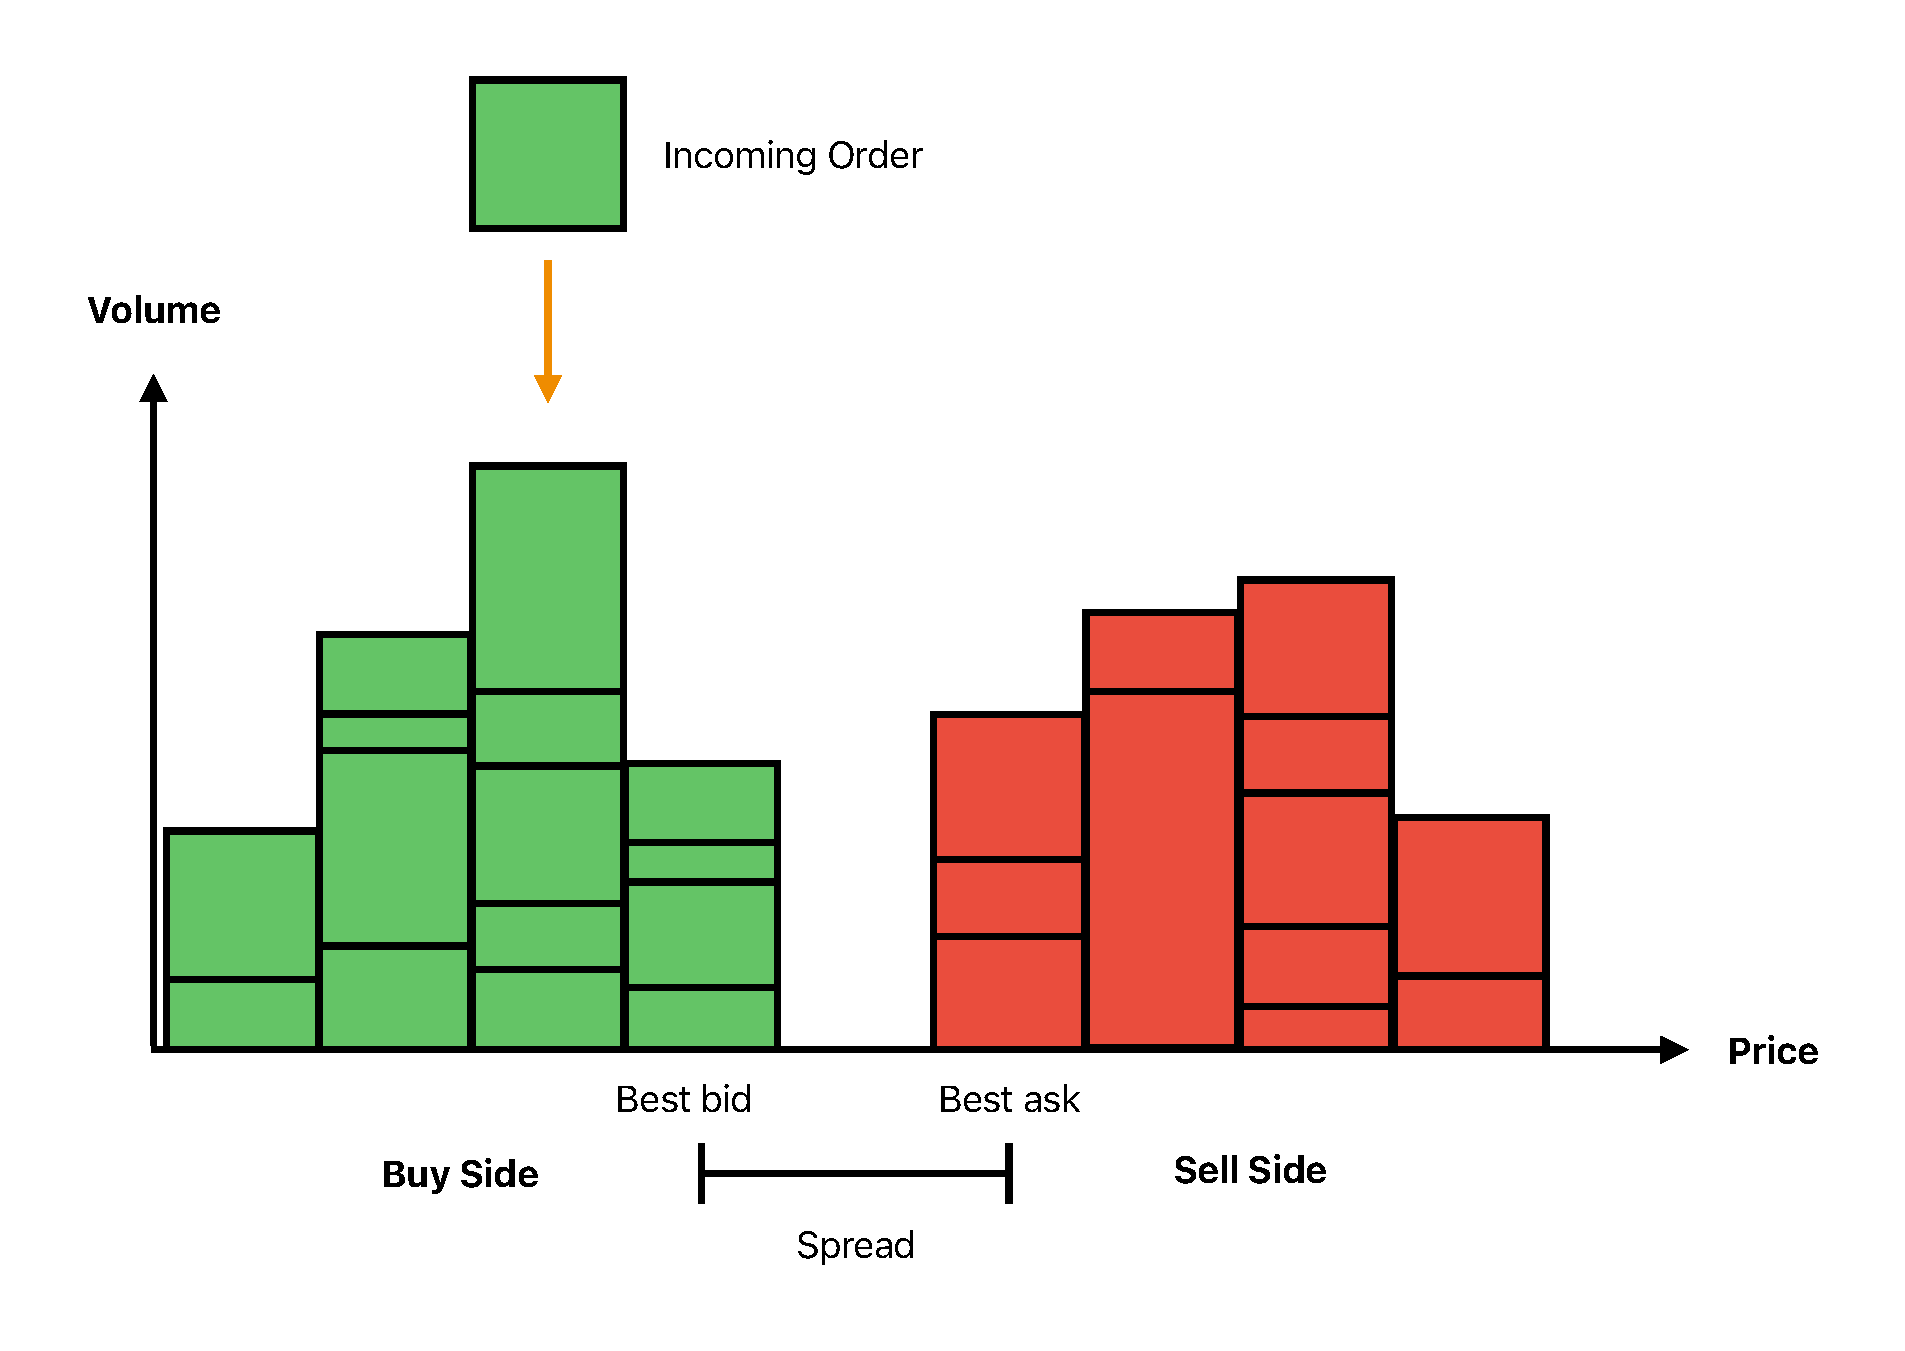
\includegraphics[height=2.5in]{LOB_Illustration.pdf}
    \caption{Limit order book snapshot illustration.}
    \label{fig:lob_illustration}
\end{figure}

Market-by-order (MBO) data offers a more granular view than standard LOB snapshots. The full sequence of messages generated at the trading venue, including order additions, cancellations, and executions, is comprised within this data. Because the entire order flow and execution messages are captured by MBO data, it can be utilized not only to reconstruct the LOB but also to extract detailed microstructure measures. The mathematical framework underpinning these representations is provided in Section~\ref{ap:matreplob} of the supplementary material, drawing heavily on \cite{cont2023mathematical, gould2013limit, panayi2015stochastic}.

In the main text, only basic notation is introduced to preserve the flow of the discussion. Let the value of a given feature $y$ at time $t \in [0, T]$ be represented by $y(t)$. As will be demonstrated in the next section, the LOB can be sampled in several ways. Two time scales are utilized: the first consists of the random times at which the LOB value is changed due to a new limit order addition, cancellation, or market order execution, by which an event-driven time series is produced. The second time scale consists of the regularly spaced observation times at which the LOB snapshot realization may be observed. A random partition \citep[Ch.~2]{Protter2005} is sufficient to distinguish between these two schemes. Random partitions are denoted as \( \mathcal{P} = \{\tau_i\}_{i=0}^N \), where \( 0 = \tau_0 \leq \tau_1 \leq \tau_2 \leq \cdots \leq \tau_N = T \) are stopping times, and \( N \) is an almost surely finite integer-valued random variable. For any random partition, let $y_i^{\mathcal{P}} = y(\tau_i)$ represent the observation of the feature $y$ at the corresponding stopping time $\tau_i$. Whenever the random partition is clear from the context, the superscript $\mathcal{P}$ will be omitted. It is noted that if the stopping times are random, $\mathcal{P}$ models the event-driven scheme; otherwise, $\mathcal{P}$ models the time-driven scheme. This distinction is further explained in Section~\ref{SubSect:SampLOB}.

Consider a trading session time interval represented by $[0, T]$, during which a sequence of orders sent by participants is observed. This order flow sequence (OFS) consists of messages denoted by $\mathbf{o} = \{o_i\}_{i=1}^{N-1}$, where each message $o_i = (p_i, z_i, t_i, i_i, s_i, k_i)$ is submitted to the matching engine at time $t_i \in [0, T]$. Here, $p_i \in \mathbb{N}_{0:d}$ denotes the price level, $z_i \in \mathbb{N}$ the size, $i_i \in \mathbb{N}$ a unique message identifier, $s_i \in \{1, -1\}$ the side of the limit order book (with $s_i = 1$ indicating the bid side and $s_i = -1$ the ask side), and $k_i \in \{L, C, M\}$ the message type (limit, cancellation, or market order, respectively). For simplicity, buy (sell) market orders in the order flow sequence $\mathbf{o}$ are identified as limit orders with the maximum (minimum) possible price. That is,

\begin{align*}
    (p_o, z_o, t_o, i_o, 1,  M) & \equiv (d, z_o, t_o, i_o, 1, L),  \\
    (p_o, z_o, t_o, i_o, -1, M) & \equiv (0, z_o, t_o, i_o, -1, L).
\end{align*}

A large number of participants interact in financial markets with a wide array of trading strategies; the aggregate process of such collections of orders can be modeled stochastically. Let $\boldsymbol{\omega} = (\omega_i : \tau_i \leq T)$ denote the Stochastic Order Flow Sequence (SOFS) where $\omega_i = (\pi_i, \zeta_i, \tau_i, \iota_i, \sigma_i, \kappa_i)$ is the random object whose realizations are given by $o_i$ (explained above). The sequence $\mathbf{o}$ is designated as the Observed Order Flow Sequence (OOFS).

The OOFS $\mathbf{o}$, together with a specified matching rule (price-time in this case), produces MBO data. There are various ways to represent this information. Table \ref{tab:db_itch_mapping} compares two such schemes: Nasdaq’s ITCH 5.0 protocol \cite{nasdaq2014itch} and the MBO data format provided by Databento\footnote{See \url{https://databento.com/docs/venues-and-datasets/xnas-itch?historical=python&live=python&reference=python}}. A key distinction between the OFS and MBO data is that the OFS itself does not reflect matching, while the MBO data is already matched according to the given matching rule. As a result, reconstructing the limit order book (LOB) from MBO data is relatively straightforward; sufficiency is achieved by maintaining two lists—one for the buy side and one for the sell side—backed by hash tables keyed by order IDs. Conversely, reconstructing the LOB directly from the OFS is more complex and computationally intensive, as it requires continuously tracking order priority in addition to storing all outstanding orders. Furthermore, incomplete OFS data is often provided by some data vendors. Approximate LOB reconstruction when only incomplete OFS data is available is discussed in Chapter 3 of \cite{richards2019modelling}.


\begin{table}[ht!]
  \caption{Message mapping of Nasdaq's ITCH (NQ) and Databento (DB) messages. The T, F, and C indicators from Databento can be interpreted as Trade, Fill, and Cancel, respectively.}
  \label{tab:db_itch_mapping}

    \centering
    \begin{tabular}{|l|l|l|l|}
        \hline
        Message description                                                          & NQ indicator & DB indicator & Remarks                                                                                                                                                                         \\ \hline
        Add Order                                                                    & A            & A            & Limit Order on Bid or Ask                                                                                                                                                       \\ \hline
        \begin{tabular}[c]{@{}l@{}}Add Order with \\ MPID \DIFdelbeginFL \DIFdelFL{attribution}\DIFdelendFL \DIFaddbeginFL \DIFaddFL{Attribution}\DIFaddendFL \end{tabular}   & F            & A            & \begin{tabular}[c]{@{}l@{}}Attribution details are \\ omitted in the DB dataset.\end{tabular}                                                                                   \\ \hline
        \begin{tabular}[c]{@{}l@{}}Order Executed \\ Message\end{tabular}            & E            & T, F, then C & \begin{tabular}[c]{@{}l@{}}All indicators share the \\ same timestamp.\end{tabular}                                                                                             \\ \hline
        \begin{tabular}[c]{@{}l@{}}Order Executed \\ with Price Message\end{tabular} & C            & T, F, then C & \begin{tabular}[c]{@{}l@{}}All indicators share the \\ same timestamp. \\ Indicator T is omitted \\ if the message is marked \\ as non-printable.\end{tabular}                  \\ \hline
        Order Cancel                                                                 & X            & C            & \begin{tabular}[c]{@{}l@{}}The \verb|quantity| column \\ specifies the number of \\ shares to be removed \\ from the order.\end{tabular}                                        \\ \hline
        Order Delete                                                                 & D            & C            & \begin{tabular}[c]{@{}l@{}}The \verb|quantity| column \\ shows the current display \\ size of  the order.\end{tabular}                                                          \\ \hline
        Order Replace                                                                & U            & C, then A    & \begin{tabular}[c]{@{}l@{}}Both indicators share the \\ same timestamp. \\ Indicator C is issued \\ with the original order \\ ID, followed by A with a \\ new ID.\end{tabular} \\ \hline
        \begin{tabular}[c]{@{}l@{}}Trade Message\\ (Non-Cross)\end{tabular}          & P            & T            & \begin{tabular}[c]{@{}l@{}}Indicates execution against \\ a non-displayable order \\ (e.g. Iceberg orders). \\ The transaction side is \\ marked as N.\end{tabular}             \\ \hline
        \begin{tabular}[c]{@{}l@{}}Cross Trade\\ Message\end{tabular}                & Q            & T            & \begin{tabular}[c]{@{}l@{}}Indicates completion of a \\ cross trade. The transaction \\ side is marked as N.\end{tabular}                                                       \\ \hline
    \end{tabular}

    
\end{table}


Finally, an array representation of the LOB is presented. The array representation is the one typically used in DL applications to the LOB (see for example \cite{kolm2024improving, Zhang_2019}). Let $p_l^b(t)$ ($p_l^a(t)$) denote the best bid (ask) price located $l$ ticks below (above) the best bid (ask) at time $t$, and let $v_l^b(t)$ ($v_l^a(t)$) denote the corresponding volume at that price level. Define the row vector $\mathbf{l}^{(L)}(t)$ to include $L + 1$ levels of limit order book information arranged in the following way:

$$
    \mathbf{l}^{(L)}(t) = [p^a_0(t), v^a_0(t), p^b_0(t), v^b_0(t), \dots, p^a_L(t), v^a_L(t), p^b_L(t), v^b_L(t)].
$$
For multiple time points $t_1, t_2, \dots, t_N$, these vectors are arranged into a matrix:

$$
    \mathbf{l}^{(L)}(t_{1:n})=\mathbf{l}(t_1, t_2, \dots, t_n) = \begin{bmatrix}
        \mathbf{l}^{(L)}(t_1) \\
        \mathbf{l}^{(L)}(t_2) \\
        \vdots                \\
        \mathbf{l}^{(L)}(t_n)
    \end{bmatrix}.
$$

%%%%%%%%%%%%%%%%%%%%%%%%%%%%%%%%%%%%%%%%%%%%%%%%%%%%%%%%%%%%%
\subsection{Sampling LOB and MBO data}
\label{SubSect:SampLOB}
%%%%%%%%%%%%%%%%%%%%%%%%%%%%%%%%%%%%%%%%%%%%%%%%%%%%%%%%%%%%%
Determining the optimal sampling scheme for high-frequency financial data remains an open question \cite{dutta2023review}.  Many researchers favor event‐driven schemes—i.e., using random stopping times tied to market events—rather than physical time-based sampling.  Indeed, some studies report that, in practice, event‐driven and uniform‐time sampling yield very similar results \cite{easley2021microstructure}. However, other work has indicated that trade time sampling, volume clock sampling or other approaches can affect the ability to discern certain statistical structure in LOB data, see discussion in \cite{koukorinis4959155memory}. Therefore, the fact that such sampling schemes \DIFdelbegin \DIFdel{is }\DIFdelend \DIFaddbegin \DIFadd{are }\DIFaddend found to not materially affect the DL based modeling approaches may be indicative of the fact that such statistical structure is not being captured adequately by such DL methods in the first place, rather than \DIFdelbegin \DIFdel{an }\DIFdelend evidence that such sampling method distinctions are inconsequential.

Multiple time scales interact when analyzing LOB and MBO data. These can be classified into event- and physical time-driven sampling schemes. Event-driven sampling schemes use market events such as trade times, order submission times, cancellation times, flash-crashes which can be effectively modeled as random stopping times. Physical time-driven sampling schemes use deterministic sampling schemes which might or might not be uniform. The sampling schemes interacting in this study are detailed below

\begin{itemize}
    \item \textbf{Event-Driven Sampling Schemes}
          \begin{itemize}
              \item \textbf{All-Events Scheme}: Samples the quantities of interest at every market event, such as when an order is added, canceled, or executed. Denote the corresponding random partition as $\mathcal{P}^{(E)} = \{\tau^{(E)}_j\}_{j=0}^{N^{(E)}}$, where $\tau^{(E)}_j$ is the time of the $j$-th event. This partition will appear in the implementation of the CNN-LSTM neural network (see Section \ref{subsec:cnn_lstm}) and the order flow imbalance calculation (see Table \ref{tab:features} in Section \ref{subsec:data_collection}).
              \item \textbf{Trades Scheme}: Samples the quantities of interest each time a trade occurs. Denote the corresponding random partition as $\mathcal{P}^{(T)} = \{\tau^{(T)}_j\}_{j=0}^{N^{(T)}}$, where $\tau^{(T)}_j$ is the time of the $j$-th trade. This partition will appear in the definition of Roll's measure, Roll's impact measure, Kyle's $\lambda$, modified Amihud's measure, and volume-synchronized probability of informed trading (see Table~\ref{tab:features} in Section~\ref{sec:data} for detailed definitions and references).
          \end{itemize}
    \item \textbf{Physical Time-Driven Sampling Schemes}
        \begin{itemize}
            \item \textbf{Uniform Sampling:} Samples the quantities of interest on a uniform partition. Denote the corresponding deterministic partition as $\mathcal{P}^{(U)}_{\delta} = \{\delta j\}_{j=0}^{N^{(U)}}$, where $\delta = T / N^{(U)}$ corresponds to a fixed sampling period. This scheme is most readily applied within the time-series econometrics framework. The uniform sampling scheme will be adopted for the Hybrid ARMAX-GARCH-DeepLOB model (see Section~\ref{subsec:armax_garch_paper}). All of the endogenous and exogenous variables in the model will be sampled according to this scheme either by temporal aggregation (i.e., integrating a quantity of interest over the duration of the time bar) or point sampling (i.e., recording the quantity exactly at the right endpoint of the time bar), as detailed in Table~\ref{tab:features}.
        \end{itemize}
\end{itemize}

In this context, the intervals defined by a partition \(\mathcal{P}\) are called \emph{bars}. While various sampling schemes such as volume bars can be defined (see Appendix \ref{ap:sampling_schemes} for detailed constructions), this work relies on two primary partitions. First, the \emph{all-events} partition \(\mathcal{P}^{(E)} = \{\tau^{(E)}_j\}_{j=0}^{N^{(E)}}\), where \(\tau^{(E)}_j\) denotes the time of the \(j\)-th market event, is employed to generate inputs for the CNN-LSTM network. Second, the \emph{time bars} partition \(\mathcal{P}^{(U)}\) is used for the hybrid model's adapter module, defined by
\[
    \tau^{(U)}_j=\delta\,j,\quad j=0,1,\dots,
\]
so that each interval \((\tau^{(U)}_{j-1},\tau^{(U)}_j]=(\delta(j-1),\delta j]\) is called a \emph{time bar}.

To capture the local stationarity inherent in MBO and LOB data, different model components are updated on three nested time scales: \emph{backbone} time bars, \emph{adapter} time bars, and \emph{sampling} time bars.  First, each trading session is uniformly partitioned into coarse backbone bars, which govern the full retraining of the global model.  Within each backbone bar, finer adapter bars are defined to schedule the adapter’s online updates. Finally, each adapter bar is subdivided into sampling bars, on which data are ingested and one‐step‐ahead forecasts are generated.

Formally, let $B^D_d$, $d = 1, 2, \dots, D$ denote the $9:45$ am to $3:45$ pm\footnote{All times in this work are EST} time interval of the $d$-th trading session in the sample. This interval is then hierarchically partitioned as follows:

\[
    \mathcal P^{(U)}_{\Delta^B}\bigl(B^D_d\bigr)
    =\{\,B^B_{d,k}:k=1,\dots,K\},
\]
where each backbone time bar \(B^B_{d,k}\) has length \(\Delta^B\).  Within each backbone time bar, the uniform partition
\[
    \mathcal P^{(U)}_{\Delta^A}\bigl(B^B_{d,k}\bigr)
    =\{\,B^A_{d,k,\ell}:\ell=1,\dots,L\},
\]
is applied to produce adapter time bars of length \(\Delta^A\).  Finally, each adapter time bar \(B^A_{d,k,i}\) is partitioned by
\[
    \mathcal P^{(U)}_{\delta}\bigl(B^A_{d,k,\ell}\bigr)
    =\{\,B^S_{d,k,i,j}:j=1,\dots,J\},
\]
yielding sampling time bars of length \(\delta\).

%%%%%%%%%%%%%%%%%%%%%%%%%%%%%%%%%%%%%%%%%%%%%%%%%%%%%%%%%%%%%
\section{Generative Feature Learning via \DIFdelbegin \DIFdel{a }\DIFdelend Deep Learning Methods: The DeepLOB and CNN-LSTM architectures}
\label{Sect:Features}
%%%%%%%%%%%%%%%%%%%%%%%%%%%%%%%%%%%%%%%%%%%%%%%%%%%%%%%%%%%%%
%%%%%%%%%%%%%%%%%%%%%%%%%%%%%%%%%%%%%%%%%%%%%%%%%%%%%%%%%%%%%
This section reviews the deep learning architectures used to extract nonlinear features from high-frequency LOB data and additional feature processing. In Section~\ref{subsec:cnn_lstm} the DeepLOB \cite{zhang2021deeplearningmarketorder} and CNN-LSTM architectures \cite{kolm2023deep} are described along with training procedures and input-output mapping. Section~\ref{subsec:feature_extraction} explains the feature processing which supports the representations used by the hybrid econometric model proposed in this paper.
%%%%%%%%%%%%%%%%%%%%%%%%%%%%%%%%%%%%%%%%%%%%%%%%%%%%%%%%%%%%%
\subsection{The CNN-LSTM Architecture}
\label{subsec:cnn_lstm}
%%%%%%%%%%%%%%%%%%%%%%%%%%%%%%%%%%%%%%%%%%%%%%%%%%%%%%%%%%%%%
The CNN-LSTM architecture, originally presented in \cite{kolm2023deep}, is a refinement of the DeepLOB neural network architecture, introduced by Zhang et al. \cite{Zhang_2019}. The DeepLOB architecture integrates convolutional, inception, and LSTM layers to impute midprice direction. Although its performance has been outpaced by more recent frameworks \cite{prata2024lob}, DeepLOB is still considered a state-of-the-art model for price direction prediction in high-frequency financial markets \cite{briola2024deep, kolm2023deep}. Several authors have investigated the factors contributing to the high accuracy of the DeepLOB architecture \cite{kolm2023deep, kolm2024improving, briola2024deep}. Particularly, Kolm et al. \cite{kolm2023deep} empirically demonstrate that removing a composite convolutional block (see Section~\ref{subsubsec:comp_conv} in the Supplementary Material) from the original DeepLOB architecture while feeding it with order flows as inputs (see Table~\ref{tab:features} in Section~\ref{subsec:data_collection}; not to be confused with the order flow sequence defined in Section~\ref{SubSect:LOB-MBO}) tends to have a positive effect on accuracy, leading to the CNN-LSTM architecture illustrated in Figure~\ref{fig:cnn_lstm_architecture} of Appendix~\ref{ap:nn_specs}.

The CNN-LSTM architecture is employed as a high-capacity nonlinear operator mapping stationary order-flow sequences into a low-dimensional latent representation. This representation is treated as a stochastic covariate process whose realizations summarize nonlinear interactions in the limit order book. Detailed architectural specifications, including layer-by-layer descriptions, filter sizes, and optimizer hyperparameters, are provided in Appendix~\ref{ap:nn_specs}.

In its original form, DeepLOB takes as input the top 10 levels of the LOB over a window of 100 events. Formally, for the all-events partition $\mathcal{P}^{(E)}$, the DeepLOB input at step $i$ is:
\[
    \tilde{\mathbf{l}}^{\mathcal{P}^{(E)}}_{i - 99 : i}
    :=
    \tilde{\mathbf{l}}^{(9)}\!\Bigl(\tau^{\mathcal{P}^{(E)}}_{i - 99}, \tau^{\mathcal{P}^{(E)}}_{i - 98}, \dots , \tau^{\mathcal{P}^{(E)}}_{i}\Bigr)
    =
    \begin{bmatrix}
        \tilde{\mathbf{l}}^{(9)}\left(\tau^{\mathcal{P}^{(E)}}_{i - 99}\right) \\
        \tilde{\mathbf{l}}^{(9)}\left(\tau^{\mathcal{P}^{(E)}}_{i - 98}\right) \\
        \vdots                                                                 \\
        \tilde{\mathbf{l}}^{(9)}\left(\tau^{\mathcal{P}^{(E)}}_{i}\right)
    \end{bmatrix}
    \in \mathbb{R}^{100 \times 40},
\]
where $\tilde{\mathbf{l}}^{(L)}(\tau^{(E)}_x)$ is a whitened (normalized) version of the original LOB data $\mathbf{l}^{(L)}(\tau^{(E)}_x)$. As pointed out in \cite{kolm2023deep}, forecasting inputs should be stationary to avoid spurious relationships \cite{granger1974spurious, phillips1986understanding}. Since the DeepLOB inputs include prices, which are inherently non-stationary, Kolm et al. \cite{kolm2023deep} show that accuracy improves when employing stationary rather than non-stationary inputs. Constructing a stationary counterpart of the DeepLOB inputs is not trivial, as the data consist of both prices and volumes. Kolm et al. \cite{kolm2023deep} achieves this by employing whitened order flows as inputs \cite{cont2013price, cont2023cross}. These inputs can be represented as
\[
    \widetilde{\mathbf{OF}}^{\mathcal{P}^{(E)}}_{i - 99:i}
    =
    \widetilde{\mathbf{OF}}^{\mathcal{P}^{(E)}}\!\bigl(\tau^{\mathcal{P}^{(E)}}_{i - 99}, \tau^{\mathcal{P}^{(E)}}_{i - 98}, \dots , \tau^{\mathcal{P}^{(E)}}_{i}\bigr)
    =
    \begin{bmatrix}
        \widetilde{\mathbf{OF}}^{(9)}_{i - 99} \\
        \widetilde{\mathbf{OF}}^{(9)}_{i - 98} \\
        \vdots                                 \\
        \widetilde{\mathbf{OF}}^{(9)}_i
    \end{bmatrix}
    \in \mathbb{R}^{100 \times 20},
\]
where $\widetilde{\mathbf{OF}}^{(L)}_i$ is a prewhitened version of the order flows (as defined in Table~\ref{tab:features} and the comments below in Section~\ref{subsec:data_collection})
\[
    \mathbf{OF}^{(L)}_i
    =
    \bigl[\,OF^a_{0, i},\;
        OF^b_{0, i},\; OF^a_{1, i},\; OF^b_{1, i},\; \dots,\; OF^a_{L, i},\; OF^b_{L, i}\bigr]
    \in \mathbb{R}^{2(L + 1)}.
\]

The original DeepLOB target variable is a ternary classification of future price movements, derived from a filtered version of the midprice. Let $m_i = \bigl(p^{a, \mathcal{P}^{(E)}}_{0,i} + p^{b, \mathcal{P}^{(E)}}_{0,i}\bigr) / 2$ denote the midprice at the $i$-th event. For a chosen horizon $h \in \mathbb{N}$,
\[
    m_i^- = \frac{1}{h}\sum_{j=0}^{h} m_{i-j},
    \quad\quad
    m_i^+ = \frac{1}{h}\sum_{j=1}^{h} m_{i+j}.
\]
Two direction scores are considered:
\[
    d_i^{(1)} := \frac{m_i^+ - m_i^-}{m_i^-},
    \quad\quad
    d_i^{(2)} := \frac{m_i^+ - m_i}{m_i}.
\]
A ternary quantization of one of these scores is then employed as a target variable in the DeepLOB architecture:
\[
    y_i =
    \begin{cases}
        -1, & d_i^{(j)} < -\theta,              \\[6pt]
        0,  & -\theta \le d_i^{(j)} \le \theta, \\[6pt]
        1,  & d_i^{(j)} > \theta,
    \end{cases},
\]
for a fixed threshold \(\theta \in (0, 1)\). While this ternary labeling is straightforward, it introduces two tuning parameters—namely the prediction horizon \(h\) used to compute \(d_i^{(j)}\) and the threshold \(\theta\). In practice, selecting values that remain robust across varying market regimes can be challenging and may lead to instability in predictive performance. Consequently, the CNN-LSTM architecture proposed in \cite{kolm2023deep} adopts a physical-time-driven midprice return with a latency correction \(\lambda \in (0, h_1)\) at multiple horizons \(h_1, h_2, \dots, h_K \in (0, \infty)\) . In that setup, the target is
\[
    \mathbf{r}^{mid}_i
    =
    \bigl(r^{mid}_{i, 1},\, r^{mid}_{i, 2},\, \dots,\, r^{mid}_{i, K}\bigr),
\]
where
\[
    r^{mid}_{i, k}
    =
    \frac{m\bigl(\tau^{\mathcal{P}^{(E)}}_i + h_k\bigr)
        - m\bigl(\tau^{\mathcal{P}^{(E)}}_i + \lambda\bigr)}{m\bigl(\tau^{\mathcal{P}^{(E)}}_i + \lambda\bigr)}.
\]
In the present application, only one forecasting horizon is used, no latency correction is applied, and the return is computed based on the micro-price \cite{gatheral2010zero}. That is, the target variable is given by the micro-return as follows
\begin{equation}
    \tilde{r}^{w, \delta}_{i}
    =
    \frac{p^w\bigl(\tau^{\mathcal{P}^{(E)}}_i + \delta\bigr) - p^w\bigl(\tau^{\mathcal{P}^{(E)}}_i\bigr)}{p^w\bigl(\tau^{\mathcal{P}^{(E)}}_i\bigr)},
    \label{eq:micro_ret_cnnlstm}
\end{equation}
where $\delta > 0$ denotes the sampling period for the overarching hybrid model (see Section~\ref{subsec:data_collection}), and
\[
    p^w(t)
    =
    \frac{v^a_0(t)\,p^b_0(t) + v^b_0(t)\,p^a_0(t)}{v^a_0(t) + v^b_0(t)}.
\]
This construction yields a continuous-valued micro-return that is directly compatible with time-series regression and volatility modeling.

As explained in Appendix~\ref{ap:nn_specs}, the CNN-LSTM network takes whitened order flow arrays $\mathbf{OF}^{\mathcal{P}^{(E)}}_{i - 99:i}$ as inputs and micro-returns $\tilde{r}_i^{w, \delta}$, as defined in expression~\eqref{eq:micro_ret_cnnlstm}, as outputs. The training loop aims to minimize the mean squared error loss

\[
    \text{Loss}(\cnnlstm, \tilde{\mathbf{r}}^{w, \delta})
    =
    \frac{1}{N^{(E)}}
    \sum_{i=1}^{N^{(E)}}
    \left(\tilde{r}_i^{w, \delta} - \cnnlstm\left(\widetilde{\mathbf{OF}}^{\mathcal{P}^{(E)}}_{i - 99:i} \right)\right)^2.
\]
Approximate minimization of this objective function is carried out through the ADAM optimizer \cite{kingma2014adam} with a learning rate of \(10^{-4}\), exponential decay rates \(\beta_1 = 0.9\) and \(\beta_2 = 0.999\), a denominator offset of \(10^{-8}\), and a batch size of \(32\). The final weights are those yielding the smallest validation loss.

At each sampling time bar, the CNN-LSTM output is measurable with respect to the $\sigma$-algebra generated by past order-flow events. Consequently, when included as a regressor in the Hybrid ARMAX–GARCH model, it satisfies the standard exogeneity conditions required for Conditional Maximum Likelihood Estimation (CMLE) under appropriate independence assumptions.

%%%%%%%%%%%%%%%%%%%%%%%%%%%%%%%%%%%%%%%%%%%%%%%%%%%%%%%%%%%%%
\subsection{Feature Processing: The Backbone Module}
\label{subsec:feature_extraction}
%%%%%%%%%%%%%%%%%%%%%%%%%%%%%%%%%%%%%%%%%%%%%%%%%%%%%%%%%%%%%

The feature processing is conducted in three steps. First, the CNN-LSTM network is trained as described in Section~\ref{subsec:cnn_lstm}. The estimated weights $\hat{\mathbf{W}}$ of the network are stored to define the embedding $\phi_{\hat{\mathbf{W}}}$, which maps the stationary order flow sequences to the latent representation of the network's penultimate layer. Second, all covariates are tested for stationarity to avoid spurious relationships \cite{granger1974spurious, phillips1986understanding}. This step applies the Augmented Dickey--Fuller (ADF) \cite{said1984testing, hamilton_time_1994, banerjee1993co}, Phillips--Perron (PP) \cite{phillips1986understanding, hamilton_time_1994, banerjee1993co}, and Kwiatkowski--Phillips--Schmidt--Shin (KPSS) \cite{kwiatkowski1992testing} tests on every non-overlapping window, summarizing rejections to guide transformations or variable eliminations. Section~\ref{ap:stationarity_testing} in the supplementary material provides further details on the assumptions, hypotheses, test statistics, and critical regions of the stationarity tests. Third, the correlation matrix of the remaining covariates is examined to identify and mitigate multicollinearity by removing variables whose pairwise correlations exceed a user-defined absolute threshold. Randomization is employed to avoid systematic bias in variable retention when strong correlation clusters are present. The highly correlated covariates are eliminated by means of a randomized greedy graph-based algorithm. These steps ensure that all covariates entering the adapter model satisfy the regularity conditions typically required to avoid spurious regression and to justify likelihood-based inference.

%%%%%%%%%%%%%%%%%%%%%%%%%%%%%%%%%%%%%%%%%%%%%%%%%%%%%%%%%%%%%
%%%%%%%%%%%%%%%%%%%%%%%%%%%%%%%%%%%%%%%%%%%%%%%%%%%%%%%%%%%%%
\section{Proposed Hybrid ARMAX-GARCH-DeepLOB Model}
\label{subsec:armax_garch_paper}
%%%%%%%%%%%%%%%%%%%%%%%%%%%%%%%%%%%%%%%%%%%%%%%%%%%%%%%%%%%%%
%%%%%%%%%%%%%%%%%%%%%%%%%%%%%%%%%%%%%%%%%%%%%%%%%%%%%%%%%%%%%
In this work, a hybrid method is developed to incorporate generative features from the DeepLOB imputations into \DIFdelbegin \DIFdel{a }\DIFdelend \DIFaddbegin \DIFadd{an }\DIFaddend econometric regression model for micro-price. This section details how this is achieved, highlighting the benefits of this approach across three factors: computational efficiency in the high-frequency settings of two-time-scale transfer learning; statistical estimation accuracy and analysis for uncertainty quantification of forecasts; and the interpretability of regression result structures.

Autoregressive Moving Average with Exogenous variables-Generalized Autoregressive Conditional Heteroskedasticity models, or ARMAX-GARCH models, are common in financial time series analysis as \DIFdelbegin \DIFdel{its structure allows }\DIFdelend \DIFaddbegin \DIFadd{their structure allows one }\DIFaddend to approximate complex dynamics by implementing a dynamic dependence of endogenous values combined with exogenous variables while allowing for a conditionally heteroskedastic volatility structure which can capture volatility clustering and leverage effects. The process $\{r_j\}_{j \in \Z}$ is said to follow an ARMAX-GARCH process if it satisfies the following equation

\begin{equation}
    \phi(B) \left( r_j - c - \mathbf{b}^T \mathbf{x}_j \right) = \theta(B) \varepsilon_j, \quad j \in \Z.
    \label{eq:armax}
\end{equation}
Here, $\phi(z) = 1 - \phi_1 z - \phi_2 z^2 - \dots - \phi_p z^p$ and $\theta(z) = 1 + \theta_1 z + \theta_2 z^2 + \dots + \theta_q z^q$ are the autoregressive and moving average polynomials, $B$ is the backshift operator, and $\{ \mathbf{x}_j \}_{j \in \Z}$ is a covariate strongly stationary process such that the innovations are independent of the history of the process. That is, $\varepsilon_j$ is independent of $\{ \mathbf{x}_j \}_{j = - \infty : j}$ for all $j \in \Z$. On its simplest form, the noise term follows a GARCH($P$, $Q$) volatility structure. Precisely, let $\{ \varepsilon_j \}_{j \in \Z}$ be a stochastic process satisfying

\begin{equation}
    \begin{cases}
        \varepsilon_j = \sigma_j \,\eta_j, \\[6pt]
        \sigma_j^2 = \omega + \sum^{Q}_{k = 1} \alpha_k \varepsilon^2_{j - k} + \sum^P_{k = 1} \beta_k \sigma_{j - k}^2,
    \end{cases}
    \label{eq:garch}
\end{equation}
where $\omega > 0$, $\alpha_k, \beta_k \geq 0$, and $\{ \eta_j\}_{j \in \Z}$, is a sequence of i.i.d. random variables with zero mean and unit variance. The last equation can be rewritten as $\theta(B) \sigma^2_j = \omega + \alpha(B) \varepsilon^2_j$ where $\alpha(z) := \sum^Q_{k = 1} \alpha_k z^k$ and $\beta(z) := 1 - \sum^P_{k = 1} \beta_k z^k$.

To ensure the stability of the processes in Eq.~\eqref{eq:armax} and \eqref{eq:garch}, and to guarantee the asymptotic efficiency of the CMLE estimators, further restrictions must be imposed on the roots of the polynomials $\alpha(\cdot)$, $\beta(\cdot)$, $\phi(\cdot)$, and $\theta(\cdot)$ (for a detailed technical discussion, see \cite{mejia2025asymptotic}). The dynamics of equation \eqref{eq:garch} can be re-expressed as

\begin{equation}
    \mathbf{z}_j = \boldsymbol{\eta}_j + \mathbf{A}_j \mathbf{z}_{j - 1},
    \label{eq:markov_rep_garch}
\end{equation}
where\footnote{For the sake of precision, note that $\boldsymbol{\eta}_j$ is a vector of length $P+Q$ whose first entry is $\omega \eta_j^2$, its $(Q+1)$-th entry is $\omega$, and all other entries are zero.}

\[
    \mathbf{z}_j =
    \begin{pmatrix}
        \varepsilon_j^2 & \varepsilon_{j - 1}^2 & \cdots & \varepsilon_{j - Q + 2}^2 & \varepsilon_{j - Q + 1}^2 & \sigma^2_{j} & \sigma^2_{j - 1} & \cdots & \sigma^2_{j - P + 2} & \sigma^2_{j - P + 1} \\
    \end{pmatrix}^T,
\]


\[
    \mathbf{\eta}_j =
    \begin{pmatrix}
        \omega \eta_j^2 & 0 & \cdots & 0 & 0 & \omega & 0 & \cdots & 0 & 0 \\
    \end{pmatrix}^T,
\]


\[
    \mathbf{A}_j =
    \begin{pmatrix}
        \alpha_1 \eta_j^2 & \alpha_2 \eta_j^2 & \cdots & \alpha_{Q - 1} \eta_j^2 & \alpha_Q \eta_j^2 & \beta_1 \eta_j^2 & \beta_2 \eta_j^2 & \cdots & \beta_{P - 1} \eta_j^2 & \beta_P \eta_j^2 \\
        1                 & 0                 & \cdots & 0                       & 0                 & 0                & 0                & \cdots & 0                      & 0                \\
        0                 & 1                 & \cdots & 0                       & 0                 & 0                & 0                & \cdots & 0                      & 0                \\
        \vdots            & \vdots            & \ddots & \vdots                  & \vdots            & \vdots           & \vdots           & \ddots & \vdots                 & \vdots           \\
        0                 & 0                 & \cdots & 1                       & 0                 & 0                & 0                & \cdots & 0                      & 0                \\
        \alpha_1          & \alpha_2          & \cdots & \alpha_{Q - 1}          & \alpha_Q          & \beta_1          & \beta_2          & \cdots & \beta_{P - 1}          & \beta_P          \\
        0                 & 0                 & \cdots & 0                       & 0                 & 1                & 0                & \cdots & 0                      & 0                \\
        0                 & 0                 & \cdots & 0                       & 0                 & 0                & 1                & \cdots & 0                      & 0                \\
        \vdots            & \vdots            & \ddots & \vdots                  & \vdots            & \vdots           & \vdots           & \ddots & \vdots                 & \vdots           \\
        0                 & 0                 & \cdots & 0                       & 0                 & 0                & 0                & \cdots & 1                      & 0
    \end{pmatrix}.
\]
 This representation for the GARCH dynamic is useful as it allows one to define via the eigen structure of the transition matrix, the stability of the time series evolution. Consider the top Lyapunov exponent, which is defined as $\rho(\mathbf{A}) = \lim_{j \rightarrow \infty} \frac{1}{j} \E \left \{  \log\norma{\mathbf{A}_j \mathbf{A}_{j - 1} \cdots \mathbf{A}_1} \right \}$ with $\norma{\cdot}$ any matrix norm in the space of $(p + q) \times (p + q)$ matrices. Then, it can be shown that a necessary and sufficient condition for the existence of a strictly stationary solution to \eqref{eq:garch} is given by $\rho(\mathbf{A}) < 0$ \citep[thm.~2.4.]{francq2019garch}. For $P = Q = 1$, the top Lyapunov exponent condition $\rho(\mathbf{A}) < 0$ reduces to $\E \left\{ \log \left( \alpha \eta_1^2 + \beta \right) \right\} < 0$. In contrast, the condition $\alpha + \beta < 1$ is necessary and sufficient for second-order stationarity \citep[thm.~2.5.]{francq2019garch}.

Ergodicity is an important property that helps ensuring desirable properties of statistical estimators \citep[see~p.~367]{francq2019garch}. Determining ergodicity in a general GARCH(\(P\), \(Q\)) process is often more complicated than establishing its stationarity. Early studies addressed mixing properties \cite{boussama1998ergodicite, carrasco2002mixing}. A straightforward application of Theorem~2.8 from \cite{straumann_quasi-maximum-likelihood_2006} demonstrates that \(\rho(\mathbf{A}) < 0\) is sufficient to guarantee the ergodicity of the process \(\{\varepsilon_j\}_{j \in \mathbb{Z}}\).

Now, assuming that $\phi(z)$ is invertible, the solution to \eqref{eq:armax} is given by
$$
    r_j = c +  \mathbf{b}^T \mathbf{x}_j + \frac{\theta(B)}{\phi(B)} \varepsilon_j = f(\dots, (\varepsilon_{j - 1}, \mathbf{x}_{j - 1}), (\varepsilon_{j}, \mathbf{x}_{j}), (\varepsilon_{j + 1}, \mathbf{x}_{j + 1}), \dots).
$$
If the joint process $\{ (\varepsilon_j, \mathbf{x}_j) \}_{j \in \Z}$ is ergodic, then so is $\{ r_j \}_{j \in \Z}$. Unfortunately, confirming the joint ergodicity of the process \(\{(\varepsilon_j, \mathbf{x}_j)\}_{j \in \mathbb{Z}}\) does not simply follow from marginal ergodicity of \(\{\varepsilon_j\}_{j \in \mathbb{Z}}\) and \(\{\mathbf{x}_j\}_{j \in \mathbb{Z}}\). Although marginal ergodicity is a necessary condition, it is not sufficient for establishing joint ergodicity. A deeper investigation into the additional requirements for joint ergodicity lies beyond the scope of this article.

The Hybrid ARMAX-GARCH-DeepLOB model shares the structure of the ARMAX-GARCH model whilst incorporating a generative feature embedding using the CNN-LSTM DL model architecture to produce interaction time series covariates from the LOB structures which effectively produces a special construction of the covariate process to combine information from the OF and the LOB.

As explained in Section~\ref{SubSect:SampLOB}, the trading session will be partitioned into nested backbone, adapter, and sampling time bars denoted $B^B_{d,k}$, $B^A_{d,k,\ell}$, and $B^S_{d,k,\ell,j}$ respectively ($B^S_{d,k,\ell,j} \subseteq B^A_{d,k,\ell} \subseteq B^B_{d,k}$). Let the micro-return in the sampling bar $B^S_{d, k, \ell, j}$ be defined as

$$
    r^w\left( B^S_{d, k, \ell, j} \right) = \frac{p^w\left( \inf B^S_{d, k, \ell, j} + \delta \right) - p^w\left( \inf B^S_{d, k, \ell, j}\right)}{p^w\left( \inf B^S_{d, k, \ell, j}\right)},
$$
where $\inf B^S_{d, k, \ell, j}$ denotes the start time (infimum) of the sampling bar interval.

Similarly, denote the set of covariates listed in Section~\ref{subsec:data_collection} available after observing the sampling time bar $B^S_{d, k, \ell, j}$ as $\mathbf{x}_{d, k, \ell, j}$. The Hybrid ARMAX-GARCH-DeepLOB model assumes that the micro-return process follows an ARMAX-GARCH stochastic process, with the covariate term provided by the embedding $\phi_{\mathbf{W}}$ (where $\mathbf{W}$ denotes the generic network weights, as opposed to the estimated weights $\hat{\mathbf{W}}$ used during inference), encoding the features generated by the last layer of the CNN-LSTM neural network as explicitly defined in the Section~\ref{subsubsec:cnn_lstm_architecture} of the Appendix. That is, for $j \in \Z$

\begin{equation}
    \begin{cases}
        \phi(B) \left( r^w \left( B^S_{d, k, \ell, j} \right) - c - \mathbf{b}_{\boldsymbol{\omega}}^T \mathbf{x}_{d, k, \ell, j - 1} - \mathbf{b}^T_{\mathbf{X}}\phi_{\mathbf{W}} \left( \widetilde{\mathbf{OF}}^{\mathcal{P}^{(E)}}_{i_{j - 1} - 99:i_{j - 1}} \right) \right) = \theta(B) \varepsilon_{d, k, \ell, j}, \\[6pt]
        \varepsilon_{d, k, \ell, j} = \sigma_{d, k, \ell, j} \,\eta_{d, k, \ell, j},                                                                                                                                                                                                                                      \\[6pt]
        \beta(B) \sigma_{d, k, \ell, j}^2 = \omega + \alpha(B) \varepsilon^2_{d, k, \ell, j}.                                                                                                                                                                                                                             \\
    \end{cases}
    \label{eq:hybrid_armax_garch}
\end{equation}
where \(\phi(z)\) and \(\theta(z)\) have roots lying outside the unit circle, \(\{\eta_{d, k, \ell, j}\}\) is an i.i.d. sequence of random variables, and $i_j = \max\left\{i : \tau^{(E)}_{i} \in B^S_{d, k, \ell, 1:j} \right\}$ is the index of the last message that took place before sampling time bar $B^S_{d, k, \ell, 1:j}$. Let \(\varepsilon_{d, k, \ell, j}\) be independent of the history of the joint covariate process \( \left\{ \left( \mathbf{x}_t, \widetilde{\mathbf{OF}}^{\mathcal{P}^{(E)}}_{i_{t} - 99:i_{t}} \right) \right\}_{t = -\infty : j - 1}\) to avoid biased estimators \citep[Ch.~9]{hamilton_time_1994}. A second option, called the parsimonious Hybrid ARMAX-GARCH-DeepLOB model, replaces the generative embedding $\phi_{\mathbf{W}}$ in Eq.~\eqref{eq:hybrid_armax_garch} entirely with the raw CNN-LSTM output. This output is denoted by $\mathrm{CNNLSTM}_{\mathbf{W}}$ to indicate its dependence on the neural network weights.

%In addition, the ergodicity of the multivariate stochastic process \(\left\{(\varepsilon_j,\mathbf{x}_{j - 1},CL_{j - 1})\right\}_{j \in \mathbb{Z}}\) is sufficient to ensure the ergodicity of the solution to \eqref{eq:hybrid_armax_garch}.

%%%%%%%%%%%%%%%%%%%%%%%%%%%%%%%%%%%%%%%%%%%%%%%%%%%%%%%%%%%%%
%%%%%%%%%%%%%%%%%%%%%%%%%%%%%%%%%%%%%%%%%%%%%%%%%%%%%%%%%%%%%
\section{\DIFdelbegin \DIFdel{Two Time Scale }\DIFdelend \DIFaddbegin \DIFadd{Two-Time-Scale }\DIFaddend Transfer Learning for Hybrid Models Construction}
\label{sec:ttstl}
%%%%%%%%%%%%%%%%%%%%%%%%%%%%%%%%%%%%%%%%%%%%%%%%%%%%%%%%%%%%%
%%%%%%%%%%%%%%%%%%%%%%%%%%%%%%%%%%%%%%%%%%%%%%%%%%%%%%%%%%%%%

The proposed framework incorporates information from the OFS and the LOB to obtain micro-return forecasts. Let $\mathbb{F}^{\boldsymbol{\omega}} = \left( \SigAl^{\boldsymbol{\omega}}(t) \right)_{t \geq 0}$ and $\mathbb{F}^{X} = \left( \SigAl^X(t) \right)_{t \geq 0}$ be the completed filtrations generated by the OFS and LOB process, respectively. The optimal forecast of the micro-return given all the information in the OFS up to the sampling time bar $B^S_{d,k,\ell,j}$ is $\E \left \{r^w\left( B^S_{d, k, \ell, j - 1} \right)  \big | \SigAl^{\boldsymbol{\omega}}\left(\sup B^S_{d, k, \ell, j - 1} \right) \right \}$, where $\sup B^S_{d, k, \ell, j - 1}$ denotes the end time (supremum) of the sampling bar interval. This forecast is typically infeasible due to the complexity of $\SigAl^{\boldsymbol{\omega}}\left(\sup B^S_{d, k, \ell, j - 1} \right)$. The optimal forecast can be approximated by combining information from the filtrations $\mathbb{F}^{\boldsymbol{\omega}}$ and $\mathbb{F}^{X}$ additively. Moreover, a correction can be applied to account for micro-return under- and over-reactions. Specifically

\begin{align*}
\E \left \{r^w\left( B^S_{d, k, \ell, j - 1} \right)  \big | \SigAl^{\boldsymbol{\omega}}\left(\sup B^S_{d, k, \ell, j - 1} \right) \right \} &\approx c + \mathbf{b}_{\boldsymbol{\omega}}^T \mathbf{x}_{d, k, \ell, j - 1} + \mathbf{b}_{\mathbf{X}}^T \phi_{\mathbf{W}} \left( \widetilde{\mathbf{OF}}^{\mathcal{P}^{(E)}}_{i_{j - 1} - 99:i_{j - 1}} \right) + \sum^{\infty}_{k = 1} \psi_k \varepsilon_{d, k, \ell,j - k}.
\end{align*}
This approximation is heuristic and motivated by conditional projection arguments; no claim of optimality is made beyond first-order approximation under the assumed information reduction. This expression motivates the use of the Hybrid ARMAX-GARCH-DeepLOB model as given in Equation \eqref{eq:hybrid_armax_garch}.

The Hybrid ARMAX-GARCH-DeepLOB employs features learned by the CNN-LSTM network to produce statistical forecasts for micro-returns. Though seemingly simple, several considerations must be addressed due to the context at hand. First, the extensive set of covariates generates multicollinearity which hampers the model stability if left unresolved. Second, the large sample size induces ill-posedness in the likelihood function which causes the failure of numerical algorithms used to compute the estimator of the Hybrid ARMAX-GARCH-DeepLOB model. Third, news affect the covariate structure which can inhibit the model's forecasting power. These issues motivate the \DIFdelbegin \DIFdel{Two Time Scale }\DIFdelend \DIFaddbegin \DIFadd{Two-Time-Scale }\DIFaddend Transfer Learning (TTSTL) Framework for Hybrid Models construction.

Inspired by the complementary learning systems (CLS) theory—where the hippocampus enables rapid adaptation and the neocortex consolidates slow, stable structure—TTSTL couples a high-capacity \emph{backbone} with a lightweight \emph{adapter}, linked by an \emph{interface} \cite{pham_continual_2024}. The backbone module (neocortex analogue) learns durable representations; the adapter module (hippocampus analogue) turns these representations into forecasts using Statistical Estimation Theory with online updates to react quickly to changing conditions. To maintain robustness, the interface enforces parsimony by learning a stable covariate set that governs the adapter’s inputs.

To formalize the transfer learning perspective, we define the learning problem on each adapter time bar as a distinct local statistical task:
\[
\mathcal{T}_{d,k,\ell} := \text{estimation of } \boldsymbol{\varphi} \text{ under local stationarity on } B^A_{d,k,\ell},
\]
where $\boldsymbol{\varphi}$ is the parameter vector of the adapter module. The backbone learns a shared representation that is reused across these tasks. The transfer occurs through parameter combination and covariate restriction, not through shared loss functions. The remainder of this section proceeds as follows: Section~\ref{subsec:ttstl_model} details the TTSTL architecture, and Section~\ref{subsec:ttstl_update} describes the update scheme.

\subsection{The TTSTL Model}
\label{subsec:ttstl_model}

Event driven Order Flow data are encoded by the backbone module via expert‐selected features (see Section~\ref{subsec:data_collection}) and a deep representation of LOB dynamics extracted through the CNN‐LSTM network (Section~\ref{subsec:cnn_lstm}).  Because retraining of the backbone is computationally intensive, prompt adaptation to market shifts cannot be achieved.  To address this limitation, the adapter is implemented as a Hybrid ARMAX‐GARCH–DeepLOB model designed for rapid online updates (Section~\ref{subsec:armax_garch_paper}).  The high dimensionality of the backbone’s output, however, can impair the adapter’s performance, necessitating an interface for model subspace selection.  Accordingly, the variable‐selection technique described in Section~\ref{subsec:covariates_selection} is applied to transform the backbone’s representation into a reduced covariate set, thereby ensuring computational efficiency and forecasting precision.

Accurately capturing arbitrary non‐stationary relationships within a single model is infeasible, as each trading session presents a continuum of heterogeneous dynamics that intensify over longer time bars. Adapter time bars, being much shorter, tend to exhibit more stable local patterns than backbone time bars. Framing the micro-return dynamics within each adapter time bar as a distinct estimation task naturally places the method within a transfer-learning paradigm.


The TTSTL framework captures locally stationary relationships by leveraging representations learned by a backbone module (see Figure~\ref{fig:ttstl}) which comprises microstructural features (see Section~\ref{subsec:data_collection}), a generative embedding (see Section~\ref{subsec:cnn_lstm}), stationarity testing, and covariance matrix analysis (see Section~\ref{subsec:feature_extraction}).  The adapter model (Section~\ref{subsec:armax_garch_paper}) is retrained at the adapter time‐bar frequency using Conditional Maximum Likelihood Estimation (CMLE; Section~\ref{subsec:cmle_props_paper}), with model parsimony controlled via model subspace selection (Section~\ref{subsec:covariates_selection}). Incoming MBO data are preprocessed into Event-Driven LOB data (denoted as EDLOB in Figure~\ref{fig:ttstl}) and Physical Time-Driven Microstructural Features (denoted as TDMF in Figure~\ref{fig:ttstl}), then stored and broadcast to all components. The backbone ingests EDLOB to train the CNN‐LSTM network, while stationarity of the TDMF series is assessed to avoid spurious relationships\footnote{As noted in Section~\ref{subsec:cnn_lstm}, CNN‐LSTM inputs are order flow measures that remain stationary at the adapter frequency; hence, their learned features are not tested for stationarity.}.  After computing the covariance matrix and eliminating redundant variables, the backbone exports both the CNN‐LSTM weights (W in Figure~\ref{fig:ttstl}) and the full covariate set (F in Figure~\ref{fig:ttstl})  (comprising the CNN‐LSTM’s final‐layer features and the variables listed in Table~\ref{tab:mbo_data} which pass the stationarity tests declared in Section~\ref{subsec:feature_extraction}).  The interface then applies the procedure of Section~\ref{subsec:covariates_selection} to reduce $F$ to a parsimonious subset $S$ (Figure~\ref{fig:ttstl}), continuously monitoring $S$ for regime shifts.  Finally, $S$ is passed to the adapter, which generates one‐step‐ahead forecasts.


\begin{figure}[H]
\centering
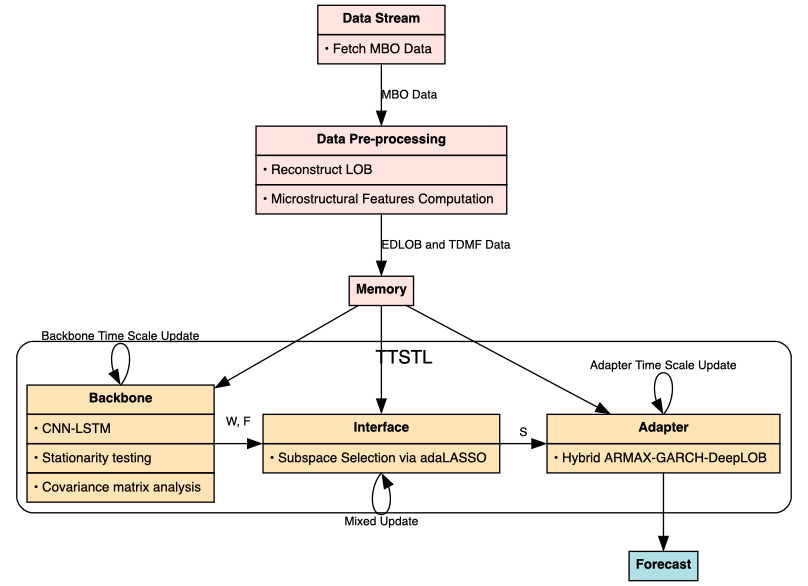
\includegraphics[height=4in]{TTSTL.png}    
\caption{\DIFdelbeginFL \DIFdelFL{Two Time Scale }\DIFdelendFL \DIFaddbeginFL \DIFaddFL{Two-Time-Scale }\DIFaddendFL Transfer Learning \DIFaddbeginFL \DIFaddFL{(TTSTL) framework}\DIFaddendFL . \DIFaddbeginFL \DIFaddFL{The diagram illustrates the interaction between the high-capacity deep learning backbone (slow-timescale feature learning), the interface module (feature embedding transfer and subspace selection via adaLASSO), and the econometric adapter module (fast-timescale calibration and parsimonious online forecasting).}\DIFaddendFL }
\label{fig:ttstl}
\end{figure}

Two operational modes are defined to manage computational cost: \textbf{Global Retrain} mode and \textbf{Local Adapt} mode (Table~\ref{tab:ttstl_modes}). In Global Retrain mode, all components—backbone, interface, and adapter—are fully updated overnight at the end of each backbone time bar. Specifically, the CNN-LSTM weights are re‐estimated, stationarity tests and covariance analyses are performed, and interface hyperparameters are tuned. The updated backbone parameters and interface settings are then carried forward into the corresponding backbone bar on the following trading day. During Local Adapt mode, the backbone weights and selected covariate subspace remain fixed; the adapter executes recursive CMLE updates at each adapter time bar to refine forecasts, while the interface uses its fixed hyperparameters solely to monitor for shifts in regression structure.

\begin{table}[ht]
  \caption{TTSTL Modes: Global Retrain vs.\ Local Adapt}
  \label{tab:ttstl_modes}

\centering
\begin{tabular}{lcc}
\toprule
\textbf{Module} & \textbf{Global Retrain mode} & \textbf{Local Adapt mode} \\
\midrule
Backbone
  & Full update
  & \begin{tabular}[t]{@{}l@{}}Transfers Learned Weights \\ Transfers Full Set of Covariates\end{tabular}\\[6pt]
Interface
  & Full update
  & Transfers Learned Hyperparameters\\[6pt]
Adapter
  & Incremental Updates
  & Incremental Updates and Forecasts\\
\bottomrule
\end{tabular}

\end{table}

\subsection{The TTSTL Updating Scheme}
\label{subsec:ttstl_update}

This section describes the updating scheme. In Global Retrain mode, the weights of the CNN-LSTM update according to the scheme given by

$$
\hat{\mathbf{W}}(B^B_{1:d, k}) = \mathrm{Update}\left(\hat{\mathbf{W}}(B^B_{1:d-1, k}), B^B_{d, k} \right).
$$
The update operator is intentionally left abstract, as the TTSTL framework is agnostic to the specific backbone optimization method. Training is performed with the Adam optimizer (Section~\ref{subsec:cnn_lstm}). Within each backbone time bar \(B^B_{d,k}\), a contiguous validation interval is selected whose length is a fixed percentage of the bar; the remaining observations constitute the training set. To prevent temporal leakage, buffer windows are inserted immediately before and after the validation block and exclude them from both training and validation.

The interface module contains four hyperparameters of interest (See Sections~\ref{subsec:covariates_selection} in the text and \ref{ap:case_study_var_selection} in the appendix for further details)\footnote{Appendix Section~\ref{ap:case_study_var_selection} is also available in repository form at \url{https://github.com/judmejiabe/case-study-adaLASSO.git}.}: $\lambda_1$, $\lambda_2$, $\alpha$ and $\tau$. In Global Retrain mode, \(\lambda_1\) and \(\alpha\) are selected via a \DIFdelbegin \DIFdel{cross validation }\DIFdelend \DIFaddbegin \DIFadd{cross-validation }\DIFaddend approach; \(\lambda_2\) and \(\tau\) are updated via a BIC approach. BIC is used heuristically to control model complexity within each backbone bar, rather than as a global consistency criterion. The resulting hyperparameters \DIFdelbegin \DIFdel{freeze }\DIFdelend \DIFaddbegin \DIFadd{are frozen }\DIFaddend during the Local Adapt mode to detect shifts in regression structure. This procedure is carried out independently of previous time bars and thus the updating scheme can ignore information from other backbone time bars.

$$
(\hat{\lambda}_1, \hat{\lambda}_2, \hat{\alpha}, \hat{\tau})(B^{B}_{1:d, k}) = (\hat{\lambda}_1, \hat{\lambda}_2, \hat{\alpha}, \hat{\tau})(B^{B}_{d, k}).
$$
The model subspace learned by the interface as described in Section~\ref{subsec:covariates_selection} goes along with the same scheme

$$
S(B^B_{1:d, k}) = S(B^B_{d, k}).
$$
The estimated CNN-LSTM weights and selected covariates give way to the reduced Hybrid ARMAX-GARCH-DeepLOB model

\begin{align*}
\phi(B)\Bigl(&r^w\bigl(B^{S}_{d,k,\ell,j}\bigr) - c 
    - \mathbf{b}_{\boldsymbol{\omega}, S(B^B_{d-1,k})}^{T}\,\mathbf{x}_{d,k,\ell,j-1} \notag\\
    &\quad - \mathbf{b}^T_{\mathbf{X}, S(B^B_{d-1,k})}\,
      \phi_{\hat{\mathbf{W}}(B^B_{1:d-1,k})}\!\left(\widetilde{\mathbf{OF}}^{\mathcal{P}^{(E)}}_{i_{j-1}-99:i_{j-1}}\right)
\Bigr) = \theta(B)\,\varepsilon_{d,k,\ell,j}.
\end{align*}
Here, $r^w(B^{S}_{d,k,\ell,j})$ denotes the micro-return in the sampling time bar in parentheses, $\mathbf{b}_{\boldsymbol{\omega, S}}$ and $\mathbf{b}_{\mathbf{X}, S}$ are the regression coefficients with a zero entry in the inactive covariates (i.e. not in $S$). The reduced Hybrid ARMAX-GARCH-DeepLOB model parameters $\boldsymbol{\varphi}_{S} = (c, \mathbf{b}_{\boldsymbol{\omega, S}}, \mathbf{b}_{\mathbf{X}, S}, \boldsymbol{\phi}, \boldsymbol{\theta}, \omega, \boldsymbol{\alpha}, \boldsymbol{\beta})$ are updated at the adapter time bar frequency according to the scheme

\begin{align*}
    \hat{\boldsymbol{\varphi}}_{S(B^B_{d-1,k})}\left(B^A_{d,k,1:\ell} \right) &= \mathrm{Update}\left(\hat{\boldsymbol{\varphi}}_{S(B^B_{d-1,k})}\left(B^A_{d,k,1:\ell-1} \right), B^A_{d,k,\ell}\right),\\
    \hat{\boldsymbol{\varphi}}_{S(B^B_{d-1,k})}\left(B^A_{d,k,1} \right) &= \hat{\boldsymbol{\varphi}}_{S(B^B_{d-1,k})}\left(B^A_{d - 1,k,1:L} \right),
\end{align*}
where the $\mathrm{Update}$ mechanism is described in Section~\ref{subsec:combining_cmles}. The hyperparameters learned by the interface module in the Global Update are employed in the Local Adapt mode to heuristically assess structural changes ex post.

%Notice how the active variables and CNN-LSTM weights are selected from the previous trading session which expose the model to structural breaks. The interface will detect breaks in the regression structure as explained in Section~\ref{subsubsec:structural_break}. 

%In such case, the state of the Hybrid ARMAX-GARCH-DeepLOB model will be restarted. Also, the covariate subset and adapter module parameters are independently re-estimated on each of the adapter time bars. That is,
% \begin{align*}
% \hat{\boldsymbol{\varphi}}^{\mathrm{break}}_{S(B^A_{d,k,\ell})}\left(B^A_{d,k,1:\ell} \right) &= \hat{\boldsymbol{\varphi}}_{S(B^A_{d,k,\ell})}\left(B^A_{d,k,\ell} \right).
% \end{align*}

%%%%%%%%%%%%%%%%%%%%%%%%%%%%%%%%%%%%%%%%%%%%%%%%%%%%%%%%%%%%%
%%%%%%%%%%%%%%%%%%%%%%%%%%%%%%%%%%%%%%%%%%%%%%%%%%%%%%%%%%%%%
\section{Estimation}
\label{Sect:Estimation}
%%%%%%%%%%%%%%%%%%%%%%%%%%%%%%%%%%%%%%%%%%%%%%%%%%%%%%%%%%%%%
%%%%%%%%%%%%%%%%%%%%%%%%%%%%%%%%%%%%%%%%%%%%%%%%%%%%%%%%%%%%%
This section is devoted to the estimation procedures for the Hybrid ARMAX-GARCH-DeepLOB model.  In Section~\ref{subsec:cmle_props_paper} the conditional maximum likelihood estimator (CMLE) is formulated.  Section~\ref{subsec:combining_cmles} introduces recursive online combining rules designed to mitigate large-sample numerical instabilities, and Section~\ref{subsec:covariates_selection} describes the interface module’s model subspace selection and structural break detection via adaptive LASSO.  Together, these estimation components complete the methodological framework for real-time forecasting under non-stationary market dynamics.


%%%%%%%%%%%%%%%%%%%%%%%%%%%%%%%%%%%%%%%%%%%%%%%%%%%%%%%%%%%%%
\subsection{Conditional Maximum Likelihood Estimation in the Hybrid ARMAX-GARCH-DeepLOB Model}
\label{subsec:cmle_props_paper}
%%%%%%%%%%%%%%%%%%%%%%%%%%%%%%%%%%%%%%%%%%%%%%%%%%%%%%%%%%%%%
The ARMAX-GARCH model is well suited for the Conditional Maximum Likelihood Estimation (CMLE) method which in the notation of Equation~\eqref{eq:armax} is defined as

$$
    \hat{\boldsymbol{\varphi}}\DIFdelbegin \DIFdel{_{CMLE, T} }\DIFdelend \DIFaddbegin \DIFadd{_{\mathrm{CMLE}, T} }\DIFaddend = \DIFdelbegin \DIFdel{\arg\max_{\boldsymbol{\varphi} \in \Phi} }%DIFDELCMD < {%%%
\DIFdelend \DIFaddbegin \underset{\boldsymbol{\varphi} \in \Phi}{\operatorname{arg\,max}} \DIFadd{\, }\DIFaddend \tilde{\mathcal{L}}_{T}\DIFdelbegin %DIFDELCMD < }%%%
\DIFdelend (\boldsymbol{\varphi}).
$$
Here, $\tilde{\mathcal{L}}_{T}$ denotes the Conditional Log-Likelihood Function which is an approximation to the Log-Likelihood Function. The formal definition is given below

\begin{align*}
     & \tilde{\mathcal{L}}_{T}(\boldsymbol{\varphi}) = \sum^T_{j = 1} \log \tilde{f}_{\boldsymbol{\varphi}}\left(r_{j} \big | r_{1: j - 1}, \mathbf{x}_{0: j - 1} \right) = \sum^T_{j = 1} \tilde{\ell}_j(\boldsymbol{\varphi}),                                                                           \\
     & \tilde{\ell}_j(\boldsymbol{\varphi}) = \log \tilde{f}_{\boldsymbol{\varphi}}\left(r_{j} \big | r_{1: j - 1}, \mathbf{x}_{0 : j - 1} \right),                                                                                                                                                        \\
     & \tilde{f}_{\boldsymbol{\varphi}}\left(r_{j} \big | r_{1: j - 1}, \mathbf{x}_{0 : j - 1} \right) = \frac{1}{\tilde{\sigma}_j(\boldsymbol{\varphi})} g\left( \frac{\tilde{\varepsilon}_j(\boldsymbol{\varphi})}{\tilde{\sigma}_j(\boldsymbol{\varphi})} \right),                                      \\
     & \tilde{\varepsilon}_j(\boldsymbol{\varphi}) = r_j - \left(c +  \mathbf{b}^T \mathbf{x}_{j - 1} + \sum^p_{k = 1} \phi_k \left(r_{j - k} - c - \mathbf{b}^T \mathbf{x}_{j - k - 1}\right) + \sum^q_{j = 1} \theta_k \tilde{\varepsilon}_{j - k}(\boldsymbol{\varphi}) \right), \hspace{2mm} j \geq 1, \\
     & \tilde{\varepsilon}_j(\boldsymbol{\varphi}) = c_j \in \R, \hspace{2mm} j = 0, -1, \dots, - \max(q, Q), \\
     & \tilde{\sigma}^2_j(\boldsymbol{\varphi}) = \omega + \sum^Q_{k = 1} \alpha_k \tilde{\varepsilon}^2_{j - k}(\boldsymbol{\varphi}) + \sum^P_{k = 1} \beta_k \tilde{\sigma}^2_{j - k}(\boldsymbol{\varphi}), \hspace{2mm} j \geq 1,                                                                     \\
     & \tilde{\sigma}^2_j(\boldsymbol{\varphi}) = c'_j \in [0, \infty), \hspace{2mm} j = 0, -1, \dots, -P.
\end{align*}
Here $g$ is the probability density function of $\eta_j$. Standard results imply that the influence of initialization constants $c_j$ and $c'_j$ vanishes asymptotically and is negligible for sufficiently long adapter windows. Several properties of \DIFdelbegin \DIFdel{$\hat{\boldsymbol{\varphi}}_{CMLE, T}$ }\DIFdelend \DIFaddbegin \DIFadd{$\hat{\boldsymbol{\varphi}}_{\mathrm{CMLE}, T}$ }\DIFaddend are given in \cite{mejia2025asymptotic}. For instance, it is shown that the residuals $\tilde{\varepsilon}_j(\cdot)$ and $\tilde{\sigma}_j(\cdot)$ uniformly converge to their \textit{infinite history} counterparts. This validates the approach taken in Section~\ref{sec:forecasting} to approximate the residuals. Some regularity conditions are sufficient to guarantee the asymptotic efficiency of the CMLE. These regularity conditions include, but are not limited to the polynomials $\phi(\cdot)$ and $\theta(\cdot)$ in equation \eqref{eq:armax} not having roots in common and such roots being outside the complex unit disk, $\alpha(\cdot)$ and $\beta(\cdot)$ in equation \eqref{eq:garch} not having roots in common, the top Lyapunov exponent being negative, and the joint process $\left\{ \left( \varepsilon_j, \mathbf{x}_j \right)  \right\}_{j \in \Z}$ being ergodic and strictly stationary. The reader is invited to consult \cite{mejia2025asymptotic} for the technical details. The main results in \cite{mejia2025asymptotic} are paraphrased below

\begin{theorem}
    Under proper conditions, it follows that
    $$
        \hat{\boldsymbol{\varphi}}\DIFdelbegin \DIFdel{_{CMLE, T} }\DIFdelend \DIFaddbegin \DIFadd{_{\mathrm{CMLE}, T} }\DIFaddend \xrightarrow[T \rightarrow \infty]{a.s.} \boldsymbol{\varphi}_0.
    $$
    \label{thm:consistency}
\end{theorem}

\begin{theorem}
    Under proper conditions, it follows that

    $$
        \sqrt{T} (\hat{\boldsymbol{\varphi}}\DIFdelbegin \DIFdel{_{CMLE, T} }\DIFdelend \DIFaddbegin \DIFadd{_{\mathrm{CMLE}, T} }\DIFaddend - \boldsymbol{\varphi}_0) \xrightarrow[T \rightarrow \infty]{\mathcal{L}} N \left(0, I^{-1}_{\boldsymbol{\varphi}_0} \right).
    $$
    Moreover, the following outer product approximation holds

    $$
        \frac{1}{T} \sum^T_{j = 1} \nabla^T_{\boldsymbol{\varphi}} \tilde{\ell}_j(\boldsymbol{\varphi}_0) \nabla_{\boldsymbol{\varphi}} \tilde{\ell}_j(\boldsymbol{\varphi}_0) \xrightarrow[T \rightarrow \infty]{a.s.} I_{\boldsymbol{\varphi}_0}.
    $$
    \label{thm:asymptotic_normality}
\end{theorem}

Although consistency and asymptotic normality are attractive estimator properties, they can become problematic in very large samples.  By consistency, the probability that \(\hat{\boldsymbol{\varphi}}_{CMLE,T}\) lies outside any arbitrarily small neighborhood of the true parameter \(\boldsymbol{\varphi}_0\) vanishes as \(T\to\infty\).  Consequently, the likelihood surface concentrates ever more sharply around \(\boldsymbol{\varphi}_0\), resembling a Dirac delta in the limit.  In practical terms, this extreme peakiness renders the log‐likelihood ill‐conditioned and numerically unstable for standard maximization algorithms.  Thus, paradoxically, the large‐sample regime that guarantees optimal asymptotic behavior also undermines the feasibility of directly applying CMLE. This challenge is addressed in the next section.


%%%%%%%%%%%%%%%%%%%%%%%%%%%%%%%%%%%%%%%%%%%%%%%%%%%%%%%%%%%%%
\subsection{Recursively Online Combining of CMLEs}
\label{subsec:combining_cmles}
%%%%%%%%%%%%%%%%%%%%%%%%%%%%%%%%%%%%%%%%%%%%%%%%%%%%%%%%%%%%%

To help overcome the instability of the numerical algorithms used for estimation present in the large sample setting and manage dynamic relationships arising from the underlying local stationarity of the process, the present work proposes to apply a recursive local estimation procedure. This procedure entails refining a global estimate with a local estimator according to an online update rule of the form

$$
    \hat{\boldsymbol{\varphi}}_S\left( B^A_{d,k,1:\ell} \right) = \mathrm{Update}\left( \hat{\boldsymbol{\varphi}}_S\left( B^A_{d,k,1:\ell - 1} \right),  B^A_{d,k,\ell} \right)
$$
Inspired by the Bayesian model-averaging framework of \cite{madigan2003bayesian}, the update rules examined in this paper construct a weighted average of recent CMLE fits—hereafter referred to as combining formulas. By averaging fresh local estimates, these methods circumvent the instability often associated with recursive estimators. The specific combining rules utilized in this work are summarized below. These update rules are heuristic and not claimed to preserve asymptotic efficiency; rather, their primary role is to ensure numerical stabilization and rapid adaptation to local market dynamics.

% \subsubsection{Combining Update Formulas} 

\begin{itemize}
    \item \textbf{Myopic Update:} If one believes that the stationarity of the process breaks beyond one adapter time bar, a reasonable alternative is to update the estimated parameter at the end of every adapter time bar
          %use the same update formula as when structural breaks happen. That is,
          $$
              \mathrm{Update}_{\mathrm{M}}\left( \hat{\boldsymbol{\varphi}}_S\left( B^A_{d,k,1:\ell - 1} \right), B^A_{d,k,\ell}  \right) = \hat{\boldsymbol{\varphi}}_S \left( B^A_{d,k,\ell} \right)
          $$
    \item \textbf{Simple Averaging:} If the sequence of estimators is close to i.i.d., an optimal choice would be to average the estimator sequence. That is,
          $$\mathrm{Update}_{\mathrm{SA}}\left( \hat{\boldsymbol{\varphi}}\left( B^A_{d,k,1:\ell - 1} \right), B^A_{d,k,\ell} \right) = \frac{\ell - 1}{\ell} \hat{\boldsymbol{\varphi}}\left( B^A_{d,k,1:\ell - 1} \right) + \frac{1}{\ell} \hat{\boldsymbol{\varphi}}\left( B^A_{d,k,\ell} \right).
          $$
    \item \textbf{Power-Law Recency Weighting:} The myopic update and simple averaging are two extremes of the local stationarity spectrum. In the middle, the LOB dynamics shift at varying rates. In this situation, one possibility is to assign a larger weight to the estimation in the most recent windows. Motivated by \cite{zhang2025onlineestimationrollingvalidation}, the following updating rule is proposed
          $$
              \mathrm{Update}_{\mathrm{PL}}\left( \hat{\boldsymbol{\varphi}}\left( B^A_{d,k,1:\ell - 1} \right), B^A_{d,k,\ell}  \right) = \frac{\sum^{\ell - 1}_{\tilde{\ell} = 1} \tilde{\ell}^{\alpha}}{\sum^{\ell}_{\tilde{\ell} = 1} \tilde{\ell}^{\alpha}} \hat{\boldsymbol{\varphi}}\left( B^A_{d,k,1:\ell - 1} \right) + \frac{\ell^{\alpha}}{\sum^{\ell}_{\tilde{\ell} = 1} \tilde{\ell}^{\alpha}}\hat{\boldsymbol{\varphi}}\left( B^A_{d,k,\ell} \right).
          $$
    \item \textbf{Exponential Smoothing:} Another alternative to capture varying degrees of local stationarity is to forget the past at a geometric rate, see \cite{cruz2015fundamental},

          $$\mathrm{Update}_{\mathrm{ES}}\left( \hat{\boldsymbol{\varphi}}\left( B^A_{d,k,1:\ell - 1} \right), B^A_{d,k,\ell}  \right) = \left( 1 - \alpha \right) \hat{\boldsymbol{\varphi}}\left( B^A_{d,k,1:\ell - 1} \right) + \alpha \hat{\boldsymbol{\varphi}}\left( B^A_{d,k,\ell} \right).
          $$
          % \item \textbf{Minimum Variance Weighted Combining:} Let $D_{\ell} = \widehat{\mathrm{Var}}\left( \hat{\boldsymbol{\varphi}} \left( B_{\ell} \right) \right) \odot I$, the diagonal of the estimated variance of the estimator in time bar $B_{\ell}$. The minimum variance weighted combining rule is given by
          % \begin{align*}
          % \mathrm{Update}_{\mathrm{MV}}\left( \hat{\boldsymbol{\varphi}}\left( B^A_{d,k,1:\ell - 1} \right), B^A_{d,k,\ell}  \right) &= \left( \sum^{\ell - 1}_{\tilde{\ell} = 1} D_{\tilde{\ell}} \right) \left( \sum^{\ell}_{\tilde{\ell} = 1} D_{\tilde{\ell}}\right)^{-1}\hat{\boldsymbol{\varphi}}\left( B^A_{d,k,1:\ell - 1} \right) + \\
          % &\hspace{20mm}\left( \sum^{\ell}_{\tilde{\ell} = 1} D_{\tilde{\ell}}\right)^{-1} \hat{\boldsymbol{\varphi}}\left( B^A_{d,k,\ell} \right).
          % \end{align*}
\end{itemize}

% \subsubsection{Recursive Update Formulas} 

% Drawing from \cite{kierkegaard2000estimating}, a series of recursive formulas can be obtained by slightly modifying the Newton Raphson and Fisher Scoring iterations. Moreover, a simple Gradient Descent algorithm can be proposed. The developement of the Online Newton Raphson (OnNR) and Online Fisher Scoring (OnFS) algorithm are analogous and thus only the derivation of the former is presented below. 


% \begin{itemize}
%     \item \textbf{Online Newton Raphson:} One iteration of the standard offline NR algorithm to solve the equation $\nabla_{\boldsymbol{\varphi}} \mathcal{L}\left( \boldsymbol{\varphi} \right) = \mathbf{0}$ is given by

%     $$
%     \Psi\left( \boldsymbol{\varphi} \right) = \boldsymbol{\varphi} - \left[ \nabla^2_{\boldsymbol{\varphi}} \mathcal{L}\left( \boldsymbol{\varphi} \right) \right]^{-1} \nabla_{\boldsymbol{\varphi}} \mathcal{L}\left( \boldsymbol{\varphi} \right). 
%     $$
%     The NR algorithm applies the operator $\Psi$ iteratively, which under some conditions results to be a contraction and the resulting sequence of $\boldsymbol{\varphi}$ converges quadratically fast. Now consider the Conditional Log-Likelihood Function $\tilde{\mathcal{L}}_{d,k,1:\ell} \left( \boldsymbol{\varphi} \right) = \sum^{\ell}_{\tilde{\ell} = 1} \mathcal{L}_{d,k,\tilde{\ell}}\left( \boldsymbol{\varphi} \right) $ and the score equations given by $\nabla_{\boldsymbol{\varphi}} \tilde{\mathcal{L}}_{d,k,1:\ell} \left( \boldsymbol{\varphi} \right) = \sum^{\ell}_{\tilde{\ell} = 1} \nabla_{\boldsymbol{\varphi}}\mathcal{L}_{d,k,\tilde{\ell}}\left( \boldsymbol{\varphi} \right) = 0$. Assume that $\hat{\boldsymbol{\varphi}}\left( B^A_{k,d,1:\ell-1} \right)$ is available and that the time bar $B^A_{d,k,\ell,j}$ has been filled. It is reasonable to take the first iteration of the NR algorithm to be

%     $$
%     \Psi\left( \hat{\boldsymbol{\varphi}}\left( B^A_{k,d,1:\ell-1} \right) \right) = \hat{\boldsymbol{\varphi}}\left( B^A_{k,d,1:\ell-1} \right) - \left[ \nabla^2_{\boldsymbol{\varphi}} \tilde{\mathcal{L}}_{d, k,1:\ell}\left( \hat{\boldsymbol{\varphi}}\left( B^A_{k,d,1:\ell-1} \right) \right) \right]^{-1} \nabla_{\boldsymbol{\varphi}} \tilde{\mathcal{L}}_{d,k,1:\ell}\left( \hat{\boldsymbol{\varphi}}\left( B^A_{k,d,1:\ell-1} \right) \right).
%     $$
%     Notice that 

%     \begin{align*}
%     \nabla_{\boldsymbol{\varphi}} \tilde{\mathcal{L}}_{d,k,1:\ell}\left( \hat{\boldsymbol{\varphi}}\left( B^A_{k,d,1:\ell-1} \right) \right) &= \sum^{\ell}_{\tilde{\ell} = 1} \nabla_{\boldsymbol{\varphi}} \tilde{\mathcal{L}}_{d,k,\tilde{\ell}}\left( \hat{\boldsymbol{\varphi}}\left( B^A_{k,d,1:\ell-1} \right) \right)\\
%     &= \nabla_{\boldsymbol{\varphi}} \tilde{\mathcal{L}}_{d,k,1:\ell - 1}\left( \hat{\boldsymbol{\varphi}}\left( B^A_{k,d,1:\ell-1} \right) \right) + \nabla_{\boldsymbol{\varphi}} \tilde{\mathcal{L}}_{d,k,\ell}\left( \hat{\boldsymbol{\varphi}}\left( B^A_{k,d,1:\ell-1} \right) \right)\\
%     &= \nabla_{\boldsymbol{\varphi}} \tilde{\mathcal{L}}_{d,k,\ell}\left( \hat{\boldsymbol{\varphi}}\left( B^A_{k,d,1:\ell-1} \right) \right)
%     \end{align*}
%     where the last equality follows from $\hat{\boldsymbol{\varphi}}\left( B^A_{k,d,1:\ell-1} \right)$ solving the scoring equations $\nabla_{\boldsymbol{\varphi}} \mathcal{L}_{d,k,1:\ell - 1}\left( \boldsymbol{\varphi} \right) = 0$. The one step iteration is then given by

%     $$
%     \Psi\left( \hat{\boldsymbol{\varphi}}\left( B^A_{k,d,1:\ell-1} \right) \right) = \hat{\boldsymbol{\varphi}}\left( B^A_{k,d,1:\ell-1} \right) - \left[ \nabla^2_{\boldsymbol{\varphi}} \tilde{\mathcal{L}}_{d, k,1:\ell}\left( \hat{\boldsymbol{\varphi}}\left( B^A_{k,d,1:\ell-1} \right) \right) \right]^{-1} \nabla_{\boldsymbol{\varphi}} \tilde{\mathcal{L}}_{d,k,\ell}\left( \hat{\boldsymbol{\varphi}}\left( B^A_{k,d,1:\ell-1} \right) \right).
%     $$
%     Approximating the Hessian matrix only with the data in the last adapters bar yields the update formula

%     \begin{align*}
%     \hat{\boldsymbol{\varphi}}\left( B^A_{k,d,1:\ell} \right) &= \hat{\boldsymbol{\varphi}}\left( B^A_{k,d,1:\ell-1} \right) - \left[ \nabla^2_{\boldsymbol{\varphi}} \tilde{\mathcal{L}}_{d, k,\ell}\left( \hat{\boldsymbol{\varphi}}\left( B^A_{k,d,1:\ell-1} \right) \right) \right]^{-1} \nabla_{\boldsymbol{\varphi}} \tilde{\mathcal{L}}_{d,k,\ell}\left( \hat{\boldsymbol{\varphi}}\left( B^A_{k,d,1:\ell-1} \right) \right)\\
%     &= \mathrm{Update}_{\mathrm{OnNR}}\left( \hat{\boldsymbol{\varphi}}\left( B^A_{d,k,1:\ell - 1} \right), B^A_{d,k,\ell}  \right).
%     \end{align*}
%     Which is akin to carrying out one NR update every time one adapter time bar fills. 

%     \textbf{Online Fisher Scoring:} The Fisher Scoring algorithm uses a similar iteration formula to the NR algorithm approximating the Hessian matrix in the NR iteration with an estimation of its expectation usually known as the Fisher's Information Matrix. Fisher Scoring is often more stable and appropriate for statistical algorithms, although some. Invoking Fisher's identity, the OnFS update formula is defined as

%     \begin{align*}
%         \hat{\boldsymbol{\varphi}}\left( B^A_{k,d,1:\ell} \right) &=\hat{\boldsymbol{\varphi}}\left( B^A_{k,d,1:\ell-1} \right) + \left[\mathcal{J}_{d,k,\ell}\left( \hat{\boldsymbol{\varphi}}\left( B^A_{k,d,1:\ell-1} \right) \right)\right]^{-1} \nabla_{\boldsymbol{\varphi}} \tilde{\mathcal{L}}_{d,k,\ell}\left( \hat{\boldsymbol{\varphi}}\left( B^A_{k,d,1:\ell-1} \right) \right).\\
%         &= \mathrm{Update}_{\mathrm{OnFS}}\left( \hat{\boldsymbol{\varphi}}\left( B^A_{d,k,1:\ell - 1} \right), B^A_{d,k,\ell}  \right).
%     \end{align*}
%     Here, 

%     $$
%     \mathcal{J}_{d,k,\ell}\left( \boldsymbol{\varphi} \right) = \sum^{J}_{j = 1} \nabla_{\boldsymbol{\varphi}}\tilde{\ell}_{d,k,\ell,j}\left( \boldsymbol{\varphi} \right) \nabla^T_{\boldsymbol{\varphi}}\tilde{\ell}_{d,k,\ell,j}\left( \boldsymbol{\varphi} \right)
%     $$
%     \textbf{Batch Gradient Descent:} Batch Gradient Descent leverages the gradient steepest ascent property to formulate an update rule. For a learning rate $\alpha>0$, the batch gradient descent is given by

%     \begin{align*}
%         \hat{\boldsymbol{\varphi}}\left( B^A_{k,d,1:\ell} \right)
%         &=\hat{\boldsymbol{\varphi}}\left( B^A_{k,d,1:\ell-1} \right) - \alpha \nabla_{\boldsymbol{\varphi}} \tilde{\mathcal{L}}_{d,k,\ell}\left( \hat{\boldsymbol{\varphi}}\left( B^A_{k,d,1:\ell-1} \right) \right)\\
%         &= \mathrm{Update}_{\mathrm{GD}}\left( \hat{\boldsymbol{\varphi}}\left( B^A_{d,k,1:\ell - 1} \right), B^A_{d,k,\ell}  \right).\\
%     \end{align*}
%     This simple update rule is fast to compute owing to the fact that no matrix inverse computation is necessary but often comes at the cost of reduced precision and slower convergence.
% \end{itemize}


% \begin{itemize}
%     \item \textbf{Recursive Predictive Error Minimization:} This method is an online version of the Predictive Error Minimization. Its update formula is given by

%     \begin{align*}
%     \mathrm{Update}\left( \hat{\boldsymbol{\varphi}}\left( B^A_{d,k,1:\ell - 1} \right), B^A_{d,k,\ell}  \right) &= \hat{\boldsymbol{\varphi}}\left( B^A_{d,k,1:\ell - 1} \right)
%     \;+\;\\
%     &\hspace{-25mm} R_{d, k, 1:\ell}^{-1}\left( \hat{\boldsymbol{\varphi}}\left( B^A_{d,k,1:\ell - 1} \right) \right)\,
%     \sum^J_{j = 1}\varepsilon_{d,k,\ell,j}\left( \hat{\boldsymbol{\varphi}}\left( B^A_{d,k,1:\ell - 1} \right) \right)\, \psi_{d,k,\ell,j}\left( \hat{\boldsymbol{\varphi}}\left( B^A_{d,k,1:\ell - 1} \right) \right)
%     \end{align*}
% Where,
%     \begin{align*}
%     R_{d, k, 1:\ell}\left( \boldsymbol{\varphi} \right) &= \sum^{\ell}_{\tilde{\ell} = 1} \sum^J_{j = 1} \psi_{d,k,\tilde{\ell},j} \left( \boldsymbol{\varphi}  \right) \psi^{T}_{d,k,\tilde{\ell},j} \left( \boldsymbol{\varphi}  \right) = R_{d, k, 1:\ell - 1}\left( \boldsymbol{\varphi} \right) + \sum^J_{j = 1} \psi_{d,k,\ell,j} \left( \boldsymbol{\varphi}  \right) \psi^{T}_{d,k,\ell,j} \left( \boldsymbol{\varphi}  \right) \,\\[6pt]
%     \psi_{d,k,\ell,j} \left( \boldsymbol{\varphi} \right) &= \nabla_{\boldsymbol{\varphi}} \tilde{\mathbf{x}}_{d,k,\ell,j} \tilde{\mathbf{b}}  \\
%     \psi_T\left( \hat{\boldsymbol{\varphi}}\left( B_{1 : \ell - 1} \right) \right),\\[6pt]
%     \epsilon_T\bigl(\hat{\theta}_{T-1}\bigr)
%     &= Y_T \;-\; X_T\bigl(\hat{\theta}_{T-1}\bigr)\,\hat{\theta}_{T-1},\\[6pt]
%     \hat{\theta}_T
%     &= \hat{\theta}_{T-1}
%     \;+\;
%     R_T^{-1}\bigl(\hat{\theta}_{T-1}\bigr)\,
%     \epsilon_T\bigl(\hat{\theta}_{T-1}\bigr)\,
%     \psi_T\bigl(\hat{\theta}_{T-1}\bigr),\\[6pt]
%     R_T\bigl(\hat{\theta}_{T-1}\bigr)
%     &= R_{T-1}\bigl(\hat{\theta}_{T-1}\bigr)
%     \;+\;
%     \psi_T\bigl(\hat{\theta}_{T-1}\bigr)\,
%     \psi_T\bigl(\hat{\theta}_{T-1}\bigr)^{\!\top}.
%     \end{align*}

%     \item \textbf{Recursice Pseudo Linear Regression:} This method is an online adaptation of the Least Squares Approach for time series. The update formula is given below 

%     \begin{align*}
%     \epsilon_T\bigl(\hat{\theta}_{T-1}\bigr)
%     &= Y_T \;-\; X_T\bigl(\hat{\theta}_{T-1}\bigr)\,\hat{\theta}_{T-1},\\[6pt]
%     \hat{\theta}_T
%     &= \hat{\theta}_{T-1}
%     \;+\;
%     R_T^{-1}\bigl(\hat{\theta}_{T-1}\bigr)\,
%     \epsilon_T\bigl(\hat{\theta}_{T-1}\bigr)\,
%     X_T\bigl(\hat{\theta}_{T-1}\bigr),\\[6pt]
%     R_T\bigl(\hat{\theta}_{T-1}\bigr)
%     &= R_{T-1}\bigl(\hat{\theta}_{T-1}\bigr)
%     \;+\;
%     X_T\bigl(\hat{\theta}_{T-1}\bigr)\,
%     X_T\bigl(\hat{\theta}_{T-1}\bigr)^{\!\top}.
%     \end{align*}
% \end{itemize}

%In principle, whilst the Hybrid ARMAX–GARCH-DeepLOB model could be estimated by a CMLE procedure. In practice, however, the log‐likelihood typically diverges to \(-\infty\) for almost all parameter values when the sample size is large, particularly at the high sampling frequencies of Section~\ref{subsec:data_collection}.  This behavior renders standard numerical maximization unstable.

%Therefore, to overcome this issue with large sample size, one may benefit from a recursive local estimation procedure. In this work, a version of recursive online estimation, motivated by ideas from \cite{madigan2003bayesian} is proposed. In this local recursive procedure, the model is fit separately on each adapter time bar, as explained in Section~\ref{sec:ttstl}, yielding a sequence of local CMLEs \(\{\hat{\theta}^{(i)}\}_{i=1}^M\).  These are then combined online to produce a time‐updated estimator \(\hat{\theta}^{(1:m)}\) after \(m\) windows. 

%Under the first approach, one assumed that each of the local estimates are approximately independent and identically distributed, then a simple and effective rule for combining is given by the historical average:
% \[
% \hat{\theta}^{(1:m)}
% \;=\;
% \frac{1}{m}\sum_{i=1}^m \hat{\theta}^{(i)}
% \;=\;
% \frac{m-1}{m}\,\hat{\theta}^{(1:m-1)} \;+\;\frac{1}{m}\,\hat{\theta}^{(m)}.
% \]
%Under a second approach in which the local estimates are assumed only to be independent but not identically distributed, which may be more reasonable given the dynamic volatility model assumed, a reasonable approach is to adopt the minimum variance combining rule. This involves considering a set of estimators combined in a weighted linear combination given by
% \[
% \hat{\theta}^{(1:m)}
% \;=\;
% \frac{1}{m}\sum_{i=1}^m w_i \hat{\theta}^{(i)}
% \]
% where the weights are given by minimizing the variance of the combined estimator, based on the variance of each local estimator ($\hat{\theta}^{(i)}$) denoted by sequence $\left\{\widehat{\sigma}_{i}^2\right\}$ which produces minimum variance combining weight, under the weight convexity constraint i.e. that all weights are positive and sum to one, given by
% \[
% w_i = \frac{\widehat{\sigma}_{i}^{-2}}{\sum_{j=1}^m\widehat{\sigma}_{j}^{-2}}
% \]
% One can select to limit $m \leq M$ where $M\in\mathbb{N}$ and this keeps a local lookback of the last $M$ estimators in the recursive combining rule.


% Lastly, as a third approach we will study the recursive approximation methods for CMLE using past sequences of estimators. Numerous approaches to recursive CMLE methods exist, for instance see Prediction Error Methods (PEM), or the Pseudo Linear regression (PLR) methods which when recursive are typically denoted as (RPLR) methods, see discussion in \cite{ljung1983theory}. In particular we consider the proposed approach derived in \cite{kierkegaard2000estimating} which is a type of RPEM approach given as outlined below.

% The local CMLE estimator is recursively updated on each window via the RPLR updating scheme derived in \cite[Eq. 25]{kierkegaard2000estimating} based on the pseudolinear model given by
% \[
% \widehat{Y}_{t|t-1} = X_t^T(\widehat{\bm{\theta}})\widehat{\bm{\theta}}
% \]
% where regressor $X$ is allowed to be static or dynamic and it may depend on parameter vector $\bm{\theta}$ and prediction error $\epsilon_t$ given by
% \[
% \epsilon_t = Y_t - \widehat{Y}_{t|t-1}
% \]
% as well as lagged values of $Y$ or $\epsilon$, and in the case of the model in this work, also exogeneous lagged regression covariates.

% Then the recursive estimator under a RPLR approach is given by
% \[
% \hat{\theta}^{(T)} = \hat{\theta}^{(T-1)} + R_T^{-1}\left(\hat{\theta}^{(T-1)}\right)\epsilon_T\left(\hat{\theta}^{(T-1)}\right)X_T^{-1}\left(\hat{\theta}^{(T-1)}\right) 
% \]
% where 
% \[
% \epsilon_T\left(\hat{\theta}^{(T-1)}\right) = Y_T - X_T\left(\hat{\theta}^{(T-1)}\right)\hat{\theta}^{(T-1)}
% \]
% and
% \[
% R_T^{-1}\left(\hat{\theta}^{(T-1)}\right) = R_{T-t}^{-1}\left(\hat{\theta}^{(T-1)}\right) + X_T\left(\hat{\theta}^{(T-1)}\right)X_T^T\left(\hat{\theta}^{(T-1)}\right)
% \]

% https://citeseerx.ist.psu.edu/document?repid=rep1&type=pdf&doi=2da9a566bb39414c8660fec2fff4cc7114fe08f6

%%%%%%%%%%%%%%%%%%%%%%%%%%%%%%%%%%%%%%%%%%%%%%%%%%%%%%%%%%%%%



\subsection{Model Subspace Selection: The Interface Module}
\label{subsec:covariates_selection}

Including all potential covariates in the ARMAX–GARCH-DeepLOB specification risks overfitting and severe multicollinearity. To address this, a two-stage variable‐selection algorithm is adopted. The technique is based on the Flexible adaLASSO of Medeiros and Mendes \cite{MEDEIROS2016255}, which retains the oracle property and model‐selection consistency even with non‐Gaussian, heteroskedastic errors\footnote{Under some regularity conditions, of course.}. Appendix \ref{ap:case_study_var_selection} presents a simulation study to illustrate the effectiveness of adaLASSO.

% Moreover, the locally stationary feature of the market dynamics introduce the possibility of structural breaks in the regression structure which could be identified by employing the oracle property of the flexible adaLASSO (see Theorem 3 in \cite{MEDEIROS2016255}).

Within the TTSTL framework, the Interface module is designed to address both of these issues. The variable selection procedure is carried out in two stages: The first stage entails defining a surrogate model with similar dynamics to that of the Hybrid ARMAX-GARCH-DeepLOB and conduct variable selection at the adapter's time bar frequency. The adaLASSO procedure is applied under the assumption of approximate local stationarity within each adapter bar. In the second stage, the statistical significance of the selected variables is assessed by means of \(t\)-tests with heteroskedasticity correction. In this last step, the variables with a relatively higher statistical significance rate are subsequently passed to the adapter for iterative re-estimation and forecasting.
\medskip

\noindent\textbf{Stage 1: Flexible adaLASSO.}  In the adapter time bar $B^A_{d, k, \ell}$, consider the following model which is a surrogate of the Hybrid ARMAX-GARCH-DeepLOB model defined in Equation~\eqref{eq:hybrid_armax_garch}.
\begin{equation}
    \begin{cases}
        r^w\left( B^S_{d, k, \ell, j} \right) = c + \sum^{p^*}_{\nu = 1} \psi_{\nu} r^w \left( B^S_{d, k, \ell, j - \nu} \right) + \mathbf{b}_{\boldsymbol{\omega}}^T \mathbf{x}_{d, k, \ell, j - 1} + \mathbf{b}^T_{\mathbf{X}}\phi_{\hat{\mathbf{W}}\left( B^B_{1:d - 1, k} \right)} \left( \widetilde{\mathbf{OF}}^{\mathcal{P}^{(E)}}_{i_{j - 1} - 99:i_{j - 1}} \right) + \varepsilon_{d, k, \ell, j}, \\[6pt]
        \varepsilon_{d, k, \ell, j} = \sigma_{d, k, \ell, j} \,\eta_{d, k, \ell, j},\\[6pt]
        \sigma_{d, k, \ell, j}^2 = \omega + \sum^{Q}_{\nu = 1} \alpha_{\nu} \varepsilon^2_{d, k, \ell, j - \nu} + \sum^P_{\nu = 1} \beta_{\nu} \sigma_{d, k, \ell, j - \nu}^2.
    \end{cases}
    \label{eq:surrogate}
\end{equation}
Now focus on a penalization of the mean equation.  Denote

\[
    \tilde{\mathbf{x}}_{d,k,\ell,j - 1}
    =
    \begin{pmatrix}
        r^w \left( B^S_{d, k, \ell, j - 1} \right)   \\
        \vdots                                       \\
        r^w \left( B^S_{d, k, \ell, j - p^*} \right) \\
        \mathbf{x}_{d, k, \ell, j - 1},              \\
        \phi_{\hat{\mathbf{W}}\left( B^B_{1:d - 1, k} \right)}\left( \widetilde{\mathbf{OF}}^{\mathcal{P}^{(E)}}_{i_{j - 1} - 99:i_{j - 1}} \right)
    \end{pmatrix},
\]
and collect the corresponding coefficients into \(\tilde{\mathbf{b}} = \left( \psi_1, \dots, \psi_{p^*}, \mathbf{b}^T_{\boldsymbol{\omega}}, \mathbf{b}^T_{\mathbf{X}}\right)^T\), so that \(r^w\left( B^S_{d,k,\ell,j} \right) = c + \tilde{\mathbf{b}}^T\tilde{\mathbf{x}}_{d, k, \ell, j - 1} + \varepsilon_{d,k,\ell, j}\). Collecting the observations and covariates into

\begin{align*}
    \mathbf{r}\left( B^A_{d, k, \ell} \right)         & = \left( r^w\left( B^S_{d, k, \ell, 1} \right), r^w\left( B^S_{d, k, \ell, 2}\right), \dots, r^w\left( B^S_{d, k, \ell, J} \right) \right)^T, \\
    \tilde{\mathbf{X}}\left( B^A_{d, k, \ell} \right) & = \left( \tilde{\mathbf{x}}_{d,k,\ell,0}, \tilde{\mathbf{x}}_{d,k,\ell,1}, \dots, \tilde{\mathbf{x}}_{d,k,\ell,J}  \right)^T
\end{align*}
such that

\begin{align*}
    \mathbf{r}\left( B^A_{d, k, \ell} \right) = c \mathbf{1} \, + \, \tilde{\mathbf{X}}\left( B^A_{d, k, \ell} \right) \tilde{\mathbf{b}} \, + \, \boldsymbol{\varepsilon}_{d, k, \ell}
\end{align*}


The Flexible adaLASSO operates by shrinking or expanding a variable-specific $\ell_1$ penalization term. This dilation is given by the relevance of the variables as determined by an initial elastic-net fit. Formally, the flexible adaLASSO is implemented in two steps as follows.

\begin{enumerate}[label=(\roman*)]
    \item \emph{Initial elastic‐net fit.}  Obtain a preliminary estimate via
          \[
              \hat{\tilde{\mathbf{b}}}^{(I)} \left( B^A_{d, k, \ell} \right)
              = \arg\min_{c, \tilde{\mathbf{b}}} \left\{
              \norma*{\mathbf{r} - c \mathbf{1} - \tilde{\mathbf{X}} \left( B^A_{d, k, \ell}\right)\tilde{\mathbf{b}}}_2^2
              \;+\;\lambda_1\left(\alpha\|\tilde{\mathbf{b}}\|_1 + \frac{1-\alpha}{2} \|\tilde{\mathbf{b}}\|_2^2\right) \right\}.
          \]
          The elastic‐net penalty mitigates multicollinearity by combining \(\ell_1\) and \(\ell_2\) shrinkage.

    \item \emph{Adaptive re‐weighting.}  Define the weights
          \(
          w_k := \aval*{\left[\hat{\tilde{\mathbf{b}}}_k^{(I)}\left( B^A_{d, k, \ell, j} \right) \right]_{k}}^{-\tau},
          \)
          with \(\tau>0\), and solve the weighted LASSO
          \[
              \hat{\tilde{\mathbf{b}}}_{\mathrm{FaL}} \left( B^A_{d, k, \ell} \right)
              = \arg\min_{c, \tilde{\mathbf{b}}} \left\{
              \norma*{\mathbf{r} - c \mathbf{1} -  \tilde{\mathbf{X}} \left( B^A_{d, k, \ell}\right)\tilde{\mathbf{b}}}_2^2
              \;+\;\lambda_2\sum_{k} w_k\,|\tilde b_k| \right\}.
          \]
          Under the conditions described in \cite{MEDEIROS2016255}, this two‐step procedure consistently identifies the true nonzero coefficients and achieves the oracle property \cite{MEDEIROS2016255}.
\end{enumerate}

As seen in Appendix~\ref{ap:case_study_var_selection} the adaLASSO effectiveness depends on the ability of the initial fit to discriminate relevant variables from irrelevant variables. Therefore the initial elastic-net fit parameters \(\lambda_1\) and \(\alpha\) must be selected carefully --as well as the adaptive re-weighting fit ones. In \cite{MEDEIROS2016255}, the authors recommend optimizing the BIC on a hyperparameter grid. Given the sheer amount of data, conducting adaLASSO on a fine four dimensional grid of \((\lambda_1, \lambda_2, \alpha, \tau)\) becomes prohibitively expensive. To mitigate this, a train/validation partition is created to measure the quality of the initial elastic-net fit hyperparameters, yielding  \(\hat{\lambda}_1 \left( B^B_{d, k} \right)\) and \(\hat{\alpha}\left( B^B_{d, k} \right)\). Fixing these hyperparameters, select \(\hat{\lambda}_2\left( B^B_{d, k} \right)\) and \(\hat{\tau}\left( B^B_{d,k} \right)\) from a grid by minimizing the average BIC across the adapter time bars contained in \(B^B_{d,k}\). This process is only carried out in Global Retrain mode. In the Local Adapt mode, transfer the learned hyperparameters from the aligned backbone time bar of the previous day. Regime shifts are flagged when the selected covariate set or coefficient significance profile changes persistently across adapter bars.

As seen in Appendix~\ref{ap:case_study_var_selection} the adaLASSO effectiveness depends on the ability of the initial fit to discriminate relevant variables from irrelevant variables. Therefore the initial elastic-net fit parameters \(\lambda_1\) and \(\alpha\) must be selected carefully --as well as the adaptive re-weighting fit ones. In \cite{MEDEIROS2016255}, the authors recommend optimizing the BIC on a hyperparameter grid. Given the sheer amount of data, conducting adaLASSO on a fine four dimensional grid of \((\lambda_1, \lambda_2, \alpha, \tau)\) becomes prohibitively expensive. To mitigate this, a train/validation partition is created to measure the quality of the initial elastic-net fit hyperparameters, yielding  \(\hat{\lambda}_1 \left( B^B_{d, k} \right)\) and \(\hat{\alpha}\left( B^B_{d, k} \right)\). Fixing these hyperparameters, select \(\hat{\lambda}_2\left( B^B_{d, k} \right)\) and \(\hat{\tau}\left( B^B_{d,k} \right)\) from a grid by minimizing the average BIC across the adapter time bars contained in \(B^B_{d,k}\). This process is only carried out in Global Retrain mode. In the Local Adapt mode, transfer the learned hyperparameters from the aligned backbone time bar of the previous day. Regime shifts are flagged when the selected covariate set or coefficient significance profile changes persistently across adapter bars.

In the Global Retrain mode, the learned Hyperparameters are used as described in Stage 2 below to finalize the model subspace selection process. In the Local Adapt mode, the learned hyperparameters are transferred to help assess the model's structure stability.
\medskip

\noindent\textbf{Stage 2: Flexible adaLASSO-OLS Screening.} Theorem 3 in \cite{MEDEIROS2016255} hints that the Flexible adaLASSO possesses the oracle property which establishes that
$$
    \sqrt{J} \left[\hat{\tilde{\mathbf{b}}}_{\mathrm{FaL},S} \left( B^A_{d, k, \ell} \right) - \tilde{\mathbf{b}}_S \right] \xrightarrow[J \rightarrow \infty]{\mathcal{L}}\\ \sqrt{J} \left[\hat{\tilde{\mathbf{b}}}_{OLS, S} \left( B^A_{d, k, \ell} \right) - \tilde{\mathbf{b}}_S\right],
$$
where $\hat{\tilde{\mathbf{b}}}_{\mathrm{FaL},S}\left( B^A_{d, k, \ell} \right)$ is the subset of non-zero coefficients in $\hat{\tilde{\mathbf{b}}}_{\mathrm{FaL,S}}\left( B^A_{d, k, \ell} \right)$\footnote{In this particular context, $x \in \R$ is non-zero if $\aval{x} > \varepsilon$ for some small $\varepsilon > 0$} and $\hat{\tilde{\mathbf{b}}}_{OLS, S}\left( B^A_{d, k, \ell} \right)$ is the $S$-restricted ordinary least squares estimator of the model in Equation~\eqref{eq:surrogate} computed on the covariates selected by the flexible adaLASSO. Under mild conditions on the covariate process and residuals (see Proposition~8.3. in \cite{hamilton_time_1994}), it can be shown that

$$
    \sqrt{J}\left[\hat{\tilde{\mathbf{b}}}_{OLS,S} \left( B^A_{d, k, \ell} \right) - \tilde{\mathbf{b}}_S \right]  \xrightarrow[J \rightarrow \infty]{\mathcal{L}} N(\mathbf{0}, V_S),
$$
where $\mathbf{I}$ is the identity matrix of size the cardinality of the set of selected variables $S$,

\begin{align*}
    V_{S} \left( B^A_{d, k, \ell} \right)
    ={} &
    \mathbf{Q}^{-1}_S\left(B^A_{d,k,\ell}\right)\mathbf{\Omega}_S\left(B^A_{d,k,\ell}\right) \, \mathbf{Q}^{-1}_S\left(B^A_{d,k,\ell}\right),
\end{align*}
and

\begin{align*}
    \mathbf{Q}_S\left(B^A_{d,k,\ell}\right)      & = \lim_{J \rightarrow \infty} \frac{1}{J}\tilde{\mathbf{X}}_{S}^T(B^A_{d,k,\ell})
    \,\tilde{\mathbf{X}}_{S}(B^A_{d,k,\ell})                                                                                                                                                                                          \\
    \mathbf{\Omega}_S\left(B^A_{d,k,\ell}\right) & = \lim_{J \rightarrow \infty} \frac{1}{J} \sum^J_{j = 1} \E \left \{ \tilde{\mathbf{x}}_{S,d,k,\ell,j} \tilde{\mathbf{x}}_{S,d,k,\ell,j}^T \varepsilon^2_{d, k, \ell, j} \right\}.
\end{align*}
Here, the subscript $S$ is used to denote that the base expression is restricted to the variables in $S$. A consistent estimator of $V_S\left( B^A_{d,k,\ell} \right)$, called the heteroskedastic-consistent covariance matrix, is given by

\begin{align*}
    \hat{V}_{\mathrm{HC},\,S} \left( B^A_{d, k, \ell} \right)
    ={} &
    J \cdot \left(\tilde{\mathbf{X}}_{S}^T(B^A_{d,k,\ell})
    \,\tilde{\mathbf{X}}_{S}(B^A_{d,k,\ell})\right)^{-1} \\
        & \times
    \left(\sum_{j=1}^J
    \tilde{\mathbf{x}}_{S,d,k,\ell,j}
    \,\tilde{\mathbf{x}}_{S,d,k,\ell,j}^T\,
    \hat{\varepsilon}^2_{d,k,\ell,j}\right)              \\
        & \times
    \left(\tilde{\mathbf{X}}_{S}^T(B^A_{d,k,\ell})
    \,\tilde{\mathbf{X}}_{S}(B^A_{d,k,\ell})\right)^{-1}.
\end{align*}

In Global Retrain mode, the adaLASSO–OLS screening is performed by conducting heteroskedasticity‐consistent \(t\)–tests on each adapter bar.  For covariate index \(\nu\), the rejection criterion is
\[
    t_{\nu,d,k,\ell} = \sqrt{J}\;
    \frac{\bigl|\,[\hat{\tilde{\mathbf b}}_{\mathrm{OLS},S(B^A_{d,k,\ell})}(B^A_{d,k,\ell})]_{\nu}\bigr|}{\bigl[\hat V_{\mathrm{HC},\,S(B^A_{d,k,\ell})}(B^A_{d,k,\ell})\bigr]_{\nu\nu}^{1/2}}
    > z_{1-\alpha/2},
\]
where \(z_{1-\alpha/2}\) denotes the \(1-\tfrac\alpha2\) quantile of the standard normal distribution.  The empirical rejection frequency is then computed across the \(\ell\) adapter bars, and covariates whose frequency exceeds a user‐specified threshold are retained.  The selected predictor set at the end of backbone bar \(B^B_{d,k}\) is denoted \(S(B^B_{d,k})\) and passed to the adapter in Local Adapt mode.  A practical rule of thumb for the screening threshold is  given by assuming that the variable-specific \(t\)-tests are i.i.d. Bernoulli variables with success probability $\alpha$ and then taking a high quantile of the Binomial distribution as ruled by the normal approximation. That is, select the $\nu$-th variable whenever
\[
    \aval*{ \left\{\ell : t_{\nu,d,k,\ell} > z_{1 - \alpha/2}\right\}} > \alpha\,L \;+\; z_{1-\gamma}\,\sqrt{L\,\alpha\,(1-\alpha)},
\]
where \(\gamma>0\) is a small constant. This screening procedure yields a set of covariates $S\left( B^B_{d,k,\ell,j} \right)$ to be used by the adapter module in the next trading session aligned backbone time bar in the Local Adapt mode.

% \subsubsection{Structural Break Detection}
% \label{subsubsec:structural_break}

% In the local adapt mode, the Flexible adaLASSO can be used as a structural break detector. In the adapter bar $B^A_{d,k,\ell}$, the variables from the previous trading session aligned backbone bar, that is $B^B_{d - 1,k}$, are used. Likewise, the hyperparameters tuned in $B^B_{d - 1, k}$, \(\left( \hat{\lambda}_1, \hat{\lambda}_2, \hat{\alpha}, \hat{\tau} \right) \left( B^B_{d - 1,k} \right)\) are plugged in the Flexible adaLASSO procedure to yield a set of covariates $S\left( B^A_{d,k,\ell} \right)$. To monitor structural breaks, a surrogate linear model with heteroskedasticity (see Equation~\eqref{eq:surrogate}) is fit on the covariate set $S\left( B^B_{d - 1, k} \right) \cup S\left( B^A_{d,k,\ell} \right)$ via OLS and the following hypotheses are constrasted for $\ell = 1, 2, \dots, L$.

% \begin{align*}
% H_{0\ell}: &\quad \mathbf{I}_{\,S\bigl(B^A_{d,k,\ell}\bigr)\setminus S\bigl(B^B_{d-1,k}\bigr)}
%   \;\tilde{\mathbf{b}}_{\,S\bigl(B^B_{d-1,k}\bigr)\cup S\bigl(B^A_{d,k,\ell}\bigr)} = \mathbf{0},\\
% H_{1\ell}: &\quad \mathbf{I}_{\,S\bigl(B^A_{d,k,\ell}\bigr)\setminus S\bigl(B^B_{d-1,k}\bigr)}
%   \;\tilde{\mathbf{b}}_{S\bigl(B^B_{d-1,k}\bigr)\cup S\bigl(B^A_{d,k,\ell}\bigr)} \neq \mathbf{0}.
% \end{align*}
% Here, $\mathbf{I}_{\,S\bigl(B^A_{d,k,\ell}\bigr)\setminus S\bigl(B^B_{d-1,k}\bigr)}$ denotes a binary diagonal matrix with ones in the diagonal entries corresponding to the covariates in the set $S\left( B^A_{d,k,\ell}\right) \setminus S\left( B^B_{d - 1, k} \right)$ and zero elsewhere. Notice the equivalence of the null hypotheses above with $H_{0\ell}:\tilde{\mathbf{b}}_{S\left( B^A_{d,k,\ell}\right) \setminus S\left( B^B_{d - 1, k} \right)} = \mathbf{0}$. The test statistic is given by

% \begin{align*}
% T_{d,k,\ell}
% &= \hat{\tilde{\mathbf{b}}}_{\mathrm{OLS},\,S\bigl(B^B_{d-1,k}\bigr)\cup S\bigl(B^A_{d,k,\ell}\bigr)}^{T}
%   \;\mathbf{I}_{\,S\bigl(B^A_{d,k,\ell}\bigr)\setminus S\bigl(B^B_{d-1,k}\bigr)}^{T}\\
% &\quad\times
%   \left[ \frac{1}{J}\;
%     \mathbf{I}_{\,S\bigl(B^A_{d,k,\ell}\bigr)\setminus S\bigl(B^B_{d-1,k}\bigr)}
%     \;\hat{V}_{\mathrm{HC},S\bigl(B^B_{d-1,k}\bigr)\cup S\bigl(B^A_{d,k,\ell}\bigl)}
%     \;\mathbf{I}_{\,S\bigl(B^A_{d,k,\ell}\bigr)\setminus S\bigl(B^B_{d-1,k}\bigr)}
%   \right]^{-1}\\
% &\quad\times
%   \mathbf{I}_{\,S\bigl(B^A_{d,k,\ell}\bigr)\setminus S\bigl(B^B_{d-1,k}\bigr)}
%   \;\hat{\tilde{\mathbf{b}}}_{\mathrm{OLS},\,S\bigl(B^B_{d-1,k}\bigr)\cup S\bigl(B^A_{d,k,\ell}\bigr)}.
% \end{align*}
% The rejection criterion is thus 

% $$
% T_{d,k,\ell} > \chi^2_{\aval*{S\bigl(B^A_{d,k,\ell}\bigr)\setminus S\bigl(B^B_{d-1,k}\bigr)}, 1 - \alpha},
% $$
% where $\chi^2_{\aval*{S\bigl(B^A_{d,k,\ell}\bigr)\setminus S\bigl(B^B_{d-1,k}\bigr)}, 1 - \alpha}$ is the $1 - \alpha$ quantile of a chi-square distribution with $\aval*{S\bigl(B^A_{d,k,\ell}\bigr)\setminus S\bigl(B^B_{d-1,k}\bigr)}$ degrees of freedom.\footnote{If $S$ is a set, $\aval*{S}$ denotes its cardinality.} One rejection alone is not sufficient to flag a structural break inside of the backbone bar because of the multiple comparisons. Just like in the variable selection approach, a threshold must be set in order to flag a structural break inside a backbone. A simple rule of thumb is to treat these tests as independent and to generate the threshold following a normal approximation of the binomial distribution. That is, flag a structural break if

% $$
% \left|\left\{ \ell : T_{d,k,\ell} > \chi^2_{\aval*{S\bigl(B^A_{d,k,\ell}\bigr)\setminus S\bigl(B^B_{d-1,k}\bigr)}, 1 - \alpha} \right\} \right| > \alpha\, L  \, + \, z_{1 - \alpha}\,\sqrt{L\,\alpha\,(1 - \alpha)}.
% $$

%The interface features a structural break detector to help identify changes in the regression structure. This is carried out through an adaptation of the CUSUM statistic. The test consists in aggregating the standardized residuals across adapter time bars and comparing against an adequate percentile of the distribution of the supremum of the paths of a Brownian motion.


% \begin{align*}
%     CUSUM_{d, k, \ell, j} = \max_{2 \leq \ell^{**} \leq \ell} \max_{1 \leq j^{**} \leq j} \aval*{\frac{1}{\sqrt{(L - 1)J}} \sum^{\ell^{**}}_{\ell^* = 2} \sum^{j^{**}}_{j^* = 1} \frac{\tilde{\varepsilon}_{d,k,\ell^*,j^*}\left( \hat{\boldsymbol{\varphi}} \left( B^A_{d, k, 1:\ell^* - 1} \right)\right)}{\tilde{\sigma}_{d,k,\ell^*,j^*}\left( \hat{\boldsymbol{\varphi}} \left( B^A_{d, k, 1:\ell^* - 1} \right)\right)}}.
% \end{align*}
% For $d = 1, 2, \dots, D$, $k = 1, 2, \dots, K$, $\ell = 2, 3, \dots, L$, $j = 1, 2, \dots J$. Notice that the first adapter time bar is burned in in order to allow the convergence of $\frac{\tilde{\varepsilon}_{d,k,\ell^*,j^*}\left( \hat{\boldsymbol{\varphi}} \left( B^A_{d, k, 1:\ell - 1} \right)\right)}{\tilde{\sigma}_{d,k,\ell^*,j^*}\left( \hat{\boldsymbol{\varphi}} \left( B^A_{d, k, 1:\ell - 1} \right)\right)}$ to its theoretical counterpart $\eta_{d, k, \ell, j}$. It can be seen that that the quantity inside $\aval{\cdot}$ above is an approximation to

% $$
% W^{L,J}_t :=\frac{1}{\sqrt{(L - 1)J}}\sum^{\ell^{**}}_{\ell^* = 2} \sum^{j^{**}}_{j^* = 1} \eta_{d, k, \ell^*, j^*}.
% $$
% Here, $L$ and $J$ are such that $\lfloor t \rfloor = \frac{(\ell^{**} - 2) J + j^{**}}{(L - 1)J}$. From Donsker's theorem it follows that the stochastic process $\mathbf{W}^{L,J} = \left( W^{L , J}_t\right)_{t \in [0, 1]}$ converges in distribution to $\mathbf{W} := \left( W_t \right)_{t \in [0, 1]}$, the standard Brownian motion. Recall from the reflection principle that 

% $$
% \Prob\left( \sup_{0 \leq s \leq 1} \aval*{W_t} > c  \right) = 2 \Prob \left( W_1 > c \right)
% $$
% With this rationale, the sequential rejection criterion is proposed to be 

% $$
% CUSUM_{d, k, \ell, j} > \sqrt{\frac{(\ell - 2) J + j}{(L - 1)J}} z_{1 - \alpha / 2}.
% $$
% where $z_{1 - \alpha / 2}$ is the $(1 - \alpha / 2)$ quantile of the standard normal distribution.

\section{Forecasting}
\label{sec:forecasting}

In Local Adapt mode, a rolling‐origin update scheme is employed \cite{meisenbacher2022review}, whereby forecasts advance one sampling bar at a time.  At each sampling bar, the estimated CNN–LSTM weights \(\mathbf{W}\), Hybrid ARMAX–GARCH–DeepLOB parameters \(\boldsymbol{\varphi}\), and covariate subset \(S\) are used to produce a one‐step‐ahead micro‐return forecast.  Once an adapter bar (comprising several sampling bars) completes, the adapter’s parameters are updated via the recursive combining rules of Section~\ref{subsec:combining_cmles}, and the process continues into the next bar. For simplicity, the first adapter time bar is used to start the recursions of the Hybrid ARMAX-GARCH model forecasting equations. Therefore no forecasts are produced for the first adapter time bar.

Figure~\ref{fig:rolling_origin} illustrates the rolling-origin update procedure within a single backbone bar divided into three adapter bars, each containing four sampling bars. Time progresses from left to right and from top row to bottom row. In the figure, dark blue cells indicate sampling bars for which data have been fully assimilated into the adapter’s parameter estimation. Light blue cells denote sampling bars for which observations have been recorded and used to generate the upcoming (orange) forecast but whose data have not yet entered the parameter update. Orange cell mark the sampling time bars for which the one‐step‐ahead forecast is being produced. White cells correspond to sampling bars that have not yet received any data and for which no forecast is produced at the time.

\begin{figure}[htb]
    \centering
    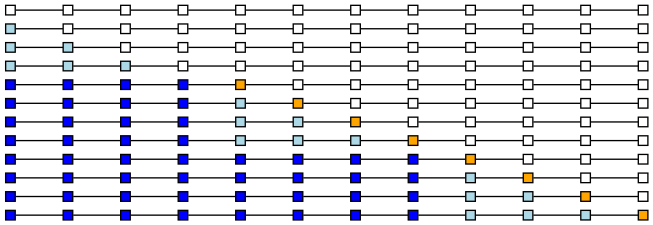
\includegraphics[height=1.25in]{rolling_origin_update_burn_in.png}
    \caption{Rolling-origin update algorithm illustration on one backbone time bar.}
    \label{fig:rolling_origin}
\end{figure}

The forecasts for the mean and volatility are produced according to a Hybrid ARMAX-GARCH-DeepLOB model. Let $d_{S,W}(B^S_{d,k,\ell,j})$ denote the part of the conditional mean which only depends on the constant term and exogenous variables. That is,

\begin{align*}
    d(B^S_{d,k,\ell,j}) & = c + \mathbf{b}_{\boldsymbol{\omega}}^{T}\,\mathbf{x}_{j-1} + \mathbf{b}^T_{\mathbf{X}}\,
    \phi_{\mathbf{W}}\!\left(\widetilde{\mathbf{OF}}^{\mathcal{P}^{(E)}}_{i_{j-1}-99:i_{j-1}}\right).
\end{align*}

The optimal forecast for the mean and the squared volatility are given by the conditional expectation and variance respectively:

\begin{align*}
    \E \left \{ r^w(B^{S}_{d,k,\ell,j}) \big| \SigAl_{d, k, \ell, j - 1} \right \}                   & =d\left( B^S_{d,k,\ell,j} \right) + \sum^p_{\nu = 1} \phi_{\nu} \left( r^w(B^{S}_{d,k,\ell,j- \nu}) - d\left( B^S_{d,k,\ell,j - \nu} \right) \right) \\
                                                                                                     & \quad+ \sum^q_{\nu = 1} \theta_{\nu} \varepsilon_{d, k, \ell, j - \nu},                                                                              \\
    \mathrm{Var}\left(r^w\left( B^S_{d, k, \ell, j}\right) \bigg| \SigAl_{d, k, \ell, j - 1} \right) & = \omega + \sum^{Q}_{\nu = 1} \alpha_{\nu} \varepsilon^2_{d,k,\ell,j - \nu} + \sum^P_{\nu = 1} \beta_{\nu} \sigma_{d, k, \ell, j - \nu}^2.
\end{align*}
Then to produce the forecast values for $r^w(B^{S}_{d,k,\ell,j})$, the parameter vector $\boldsymbol{\varphi}$ is replaced by its estimate $\hat{\boldsymbol{\varphi}}_{S\left(B^B_{d - 1, k}\right)}\left( B^A_{d,k,1:\ell - 1} \right)$ and the residuals $\varepsilon_{d,k,\ell,j}$ are estimated with $\tilde{\varepsilon}_{d,k,\ell,j} \left( \hat{\boldsymbol{\varphi}}_{S\left(B^B_{d - 1, k}\right)}\left( B^A_{d,k,1:\ell - 1} \right) \right)$ (see Section~\ref{subsec:cmle_props_paper}) using the data in the previous adapter time bar as a burn-in to help guarantee convergence of the estimated residuals.


% , then $\varepsilon_{d,k,\ell,j}$ is estimated with $\tilde{\varepsilon}_{d,k,\ell,j} \left( \hat{\boldsymbol{\varphi}}_{S\left(B^B_{d - 1, k}\right)}\left( B^A_{d,k,1:\ell - 1} \right) \right)$ (see Section~\ref{subsec:cmle_props_paper}) with starting values given by the estimated residuals in the previous adapter time bar.



% \[
% \tilde{\varepsilon}_{d,k,\ell,j}\left(\hat{\varphi}_{S(B^B_{d-1,k})}(B^A_{d,k,1:\ell})\right)
% =
% \begin{cases}
% 0, 
% & k = \ell = 1,\\
% \tilde{\varepsilon}_{d, k - 1,L,J + j}\left(\hat{\varphi}_{S(B^B_{d-1,k - 1})}(B^A_{d,k - 1,1:L - 1})\right),
% & k \geq 2, \ell = 1,\\
% \tilde{\varepsilon}_{d, k,\ell - 1,J + j}\left(\hat{\varphi}_{S(B^B_{d-1,k})}(B^A_{d,k ,1:\ell - 2})\right),
% & \ell \geq 2.
% \end{cases}
% \]
% For $j = -1, -2, \dots, -\max\{P, Q\}$. Similarly, the initial values for the volatility process are given by
% \[
% \tilde{\sigma}^2_{d,k,\ell,j}\left(\hat{\varphi}_{S(B^B_{d-1,k})}(B^A_{d,k,1:\ell - 1})\right)
% =
% \begin{cases}
% \displaystyle
% \frac{1}{J}\sum_{\tilde{j}=1}^J
% \tilde{\varepsilon}^2_{d, k - 1,L - 1,J + j}\left(\hat{\varphi}_{S(B^B_{d-1,k - 1})}(B^A_{d,k - 1,1:L - 2})\right),
% & k = \ell = 1,\\
% \tilde{\sigma}^2_{d, k - 1,L,J + j}\left(\hat{\varphi}_{S(B^B_{d-1,k - 1})}(B^A_{d,k - 1,1:L - 1})\right),
% & k \geq 2, \ell = 1,\\
% \tilde{\sigma}^2_{d, k,\ell - 1,J + j}\left(\hat{\varphi}_{S(B^B_{d-1,k})}(B^A_{d,k ,1:\ell - 2})\right),
% & \ell \geq 2.
% \end{cases}
% \]
% For $j = -1, -2, \dots, -\max\{P, Q\}$.

\section{Performance Measures}
\label{sec:performance_measures}

The selection of performance metrics in forecasting is a topic of contentious debate though empirical evidence suggests that most reasonable measures tend to rank systems similarly \cite{Koutsandreas2021}. To evaluate the predictive accuracy of the proposed framework, this study employs the Relative Mean Absolute Error ($\mathrm{RelMAE}$), computed for each adapter time bar. This metric quantifies the performance of the model relative to a benchmark by normalizing the Mean Absolute Error (MAE) of the model against that of a baseline. For a given adapter time bar $B^A_{d, k, \ell}$, it is defined as:

\[
    \mathrm{RelMAE}\left( B^A_{d, k, \ell} \right)
    \;=\;
    \frac{\displaystyle\sum_{j=1}^{J} \aval*{\tilde{\varepsilon}_{d, k, \ell, j}\left( \hat{\boldsymbol{\varphi}} \left( B^A_{d,k,1:\ell - 1} \right) \right)}}{\displaystyle\sum_{j=1}^{J} \aval*{\hat{\varepsilon}^b_{d, k, \ell, j}}}
    \;=\;
    \frac{\mathrm{MAE}\left( B^A_{d, k, \ell} \right)}{\mathrm{MAE}_{b}\left( B^A_{d, k, \ell} \right)},
\]
where $\tilde{\varepsilon}_{d, k, \ell, j}$ represents the residuals of the Hybrid ARMAX-GARCH-DeepLOB model, and $\hat{\varepsilon}^b_{d, k, \ell, j}$ represents the residuals of the chosen baseline.

Two distinct baselines are employed to assess different aspects of model performance:

\begin{enumerate}
    \item \textbf{Naive Baseline ($\hat{\varepsilon}^{b,1}$):} To assess the value added by the modeling framework over a trivial predictor, the average micro-return from the corresponding backbone bar of the previous trading session is used as the naive benchmark. The residuals for this baseline are given by:
          \begin{align*}
              \hat{\varepsilon}^{b, 1}_{d,k,\ell,j} & = r^w\bigl(B^S_{d,k,\ell,j}\bigr) \;-\; \bar{r}^w\bigl(B^B_{d - 1, k}\bigr),         \\
              \bar{r}^w\bigl(B^B_{d - 1, k}\bigr)   & = \frac{1}{JL} \sum_{\ell = 1}^L \sum_{j = 1}^J r^w\bigl(B^S_{d - 1,k,\ell,j}\bigr).
          \end{align*}

    \item \textbf{Neural Baseline ($\hat{\varepsilon}^{b,2}$):} To quantify the adapter module ability to adapt the neural network imputation, the raw imputation generated by the CNN-LSTM backbone is used as a baseline for complementary analysis. Its residuals are defined as:
          \begin{align*}
              \hat{\varepsilon}^{b, 2}_{d,k,\ell,j} & = r^w\bigl(B^S_{d,k,\ell,j}\bigr) \;-\; \mathrm{CNNLSTM}_{\mathbf{W}}\!\left(\widetilde{\mathbf{OF}}^{\mathcal{P}^{(E)}}_{i_{j-1}-99:i_{j-1}}\right).
          \end{align*}
\end{enumerate}


\section{Data}
\label{sec:data}

\subsection{Data Collection}
\label{subsec:data_collection}

Choosing the sampling frequency remains an open design choice \cite{dutta2023review}. The workflow in Figure~\ref{fig:ttstl} relies on two sampling scales: An event-driven stream providing order-flow imbalances (OFIs) and the micro-price; and a physical-time series containing all features listed in Table~\ref{tab:features}.

For the physical-time series,the sampling time bar width is set to $\delta=100$ units of time (uot) in synthetic experiments and to $\delta=2$ seconds in market-data experiments (see Section~\ref{subsec:dataset}). Table~\ref{tab:features} summarizes the measurements produced by the market-replay algorithm plus the VIX index measurements. To lighten notation, unless stated otherwise, the subscript $j$ denotes the feature evaluated on sampling bar $B^{S}_{d,k,\ell,j}$. For stock features—i.e., covariates measured at a single time point—the observation is timestamped at the right endpoint of the corresponding sampling bar.

%For the dataset obtained from the data vendor, a stock-specific approach, inspired by \cite{kolm2023deep, kolm2024improving}, is used. Specifically, the uniform sampling rate  is defined in proportion to the average time between midprice changes:

% \[
% \delta = \kappa \frac{T}{N},
% \]
% where \(T\) denotes the duration of a trading session, \(N\) is the number of midprice changes within the session, and \(\kappa \in (0, \infty)\) regulates the sampling frequency. Table~\ref{tab:features} summarizes the measures recorded using the market replay algorithm. For notation lightness and unless specified otherwise, the subscript $j$ in the features below identify correspond to the feature observed in the sampling time bar $B^S_{d,k,\ell,j}$. For stock features (i.e. covariates measured at a point in time) take the measurement time to be the right endpoint of the sampling time bar.


% Consequently, let $[0, T)$ denote the interval studied within a trading day, $\Delta$ the sampling rate, and $W$ the window size. To illustrate further, take the volume weighted mid-quote or micro-price \cite{gatheral2010zero}

% $$
% p^w(t) = \frac{v^a_0(t) p^b_0(t) + v^b_0(t) p^a_0(t)}{v^a_0(t) + v^b_0(t)}, \hspace{2mm} t \in [0, T).
% $$

% Note that $p^w(t)$ is a quantity that can be computed at any $t \in [0, T)$ by just observing the LOB at $t$. To implement the time series regression models proposed here, the target variables and covariates will be sampled at an equally spaced frequency $\delta$. In the micro-price example, this means that the random variables $p^w_n := p^w(\delta n)$ for $n \in \{ 0, 1, \dots, \lfloor \frac{T}{\delta} \rfloor + 1 \}$ will be sampled from the market replay algorithm. For practicality, the subscript notation (e.g. $p^w_t$) will indicate the $n$-th sample of a continuous time stochastic process sampled at equally spaced intervals (e.g. $p^w_t = p^w(\delta t)$).

% The following table summarizes the target variables of the models described below. The interest is not to only model the return as measured per the weighted price to discover factors that drive this quantity but also to determine the factors that drive liquidity and information asymmetry by modeling the bid-ask spread and available volume as proxy measures of these concepts. There is a wealth of literature on the factors that impact price and liquidity. Table \ref{tab:exogenous_vars} indicates the candidate variables for covariates. Observe that the number of covariates and its correlated nature would damage the stability of the time series regression models and hence the need for a feature extraction process and a model subspace selection.


\begin{longtable}{|p{4cm}|p{2.25cm}|p{5.25cm}|p{2.25cm}|}
    \caption{List of extracted microstructural measures. In this table, $\star \in \{ a, b\}$ denotes the side of the LOB, $h \in \{ 0, 1, \dots, H\}$ denotes the number of ticks away from best bid or ask values, and $t \in \{ 1, \dots, kN \}$ corresponds to the sequence in the time partition $\mathcal{P}^{(U)}_{\delta} = \{ \delta j \}^{k N}_{t = 1}$.} \label{tab:features} \\ \hline
    \textbf{Feature Name}                                                                                                                                                  & \textbf{Notation}     & \textbf{Definition}                                                                                                                                                 & \textbf{References} \\ \hline
    \endfirsthead
    \caption*{Table \ref{tab:features} (continued)}                                                                                                                                                                                                                                                                                                                                            \\
    \hline
    \textbf{Feature Name}                                                                                                                                                  & \textbf{Notation}     & \textbf{Definition}                                                                                                                                                 & \textbf{References} \\ \hline
    \endhead
    \hline
    \endfoot
    \hline
    \endlastfoot

    % Timestamp & 
    % $TOD_j$ & 
    % \begin{tabular}[t]{@{}l@{}}Measurement's physical \\ time (i.e. $\delta j$) \end{tabular} & 
    % \cite{kolm2024improving} \\ \hline

    $l$-th best bid (ask)                                                                                                                                                  &
    $p^{\star}_{l,j}$                                                                                                                                                      &
    $l$-th best price on side $\star$                                                                                                                                      &
    \cite{briola2024deep}                                                                                                                                                                                                                                                                                                                                                                      \\ \hline

    Available volume on side $\star$ and depth $l$                                                                                                                         &
    $v^{\star}_{l,j}$                                                                                                                                                      &
    \begin{tabular}[t]{@{}l@{}}Volume sitting at the \\ $l$-th best price on side $\star$.\end{tabular}                                                                    &
    \cite{briola2024deep}                                                                                                                                                                                                                                                                                                                                                                      \\ \hline

    Spread                                                                                                                                                                 &
    $s_j$                                                                                                                                                                  &
    $p^b_{0, j} - p^a_{0, j}$.                                                                                                                                             &
    \cite{hasbrouck1991measuring, easley2021microstructure}                                                                                                                                                                                                                                                                                                                                    \\ \hline

    Micro-price                                                                                                                                                            &
    $p^w_j$                                                                                                                                                                &
    $\frac{v^a_{0, j} p^b_{0, j} + v^b_{0, j} p^a_{0, j}}{v^a_{0, j} + v^b_{0, j}}$.                                                                                       &
    \cite{gatheral2010zero}                                                                                                                                                                                                                                                                                                                                                                    \\ \hline

    % CNN-LSTM output & 
    % $CL_j$ & 
    % $CL(TOD_j)$. & 
    % \cite{Zhang_2019} \\ \hline

    Actual LOB depth                                                                                                                                                       &
    $\Xi^{\star}_j$                                                                                                                                                        &
    $\big| p^{\star}_{L, j} - p^{\star}_{0, j} \big|$.                                                                                                                     &
    \cite{briola2024deep}                                                                                                                                                                                                                                                                                                                                                                      \\ \hline

    Imbalance in trading volume                                                                                                                                            &
    $\rho_j$                                                                                                                                                               &
    $\frac{v^b_{0, j} - v^a_{0, j}}{v^b_{0, j} + v^a_{0, j}}$.                                                                                                             &
    \cite{cartea2018enhancing}                                                                                                                                                                                                                                                                                                                                                                 \\ \hline

    Bid order flow                                                                                                                                                         &
    $OF^b_{l, j}$                                                                                                                                                          &
    \begin{tabular}[t]{@{}l@{}}$\begin{cases} v^b_{l, j}                  & p^b_{l, j} > p^b_{l, j - 1}, \\
              v^b_{l, j} - v^b_{l, j - 1} & p^b_{l, j} = p^b_{l, j - 1}, \\
              -v^b_{l, j -1}              & p^b_{l, j} < p^b_{l, j - 1}.\end{cases}$\end{tabular}                                                                                                   &
    \cite{cont2013price, kolm2023deep}                                                                                                                                                                                                                                                                                                                                                         \\ \hline

    Ask order flow                                                                                                                                                         &
    $OF^a_{l, j}$                                                                                                                                                          &
    \begin{tabular}[t]{@{}l@{}}$\begin{cases} v^a_{l, j}                  & p^a_{l, j} < p^a_{l, j - 1}, \\
              v^a_{l, j} - v^a_{l, j - 1} & p^a_{l, j} = p^a_{l, j - 1}, \\
              -v^a_{l, j -1}              & p^a_{l, j} > p^a_{l, j - 1}.\end{cases}$\end{tabular}                                                                                                   &
    \cite{cont2013price, kolm2023deep}                                                                                                                                                                                                                                                                                                                                                         \\ \hline

    Order flow imbalance                                                                                                                                                   &
    $OFI_{l, j}$                                                                                                                                                           &
    $\sum_{i \in I_j} OF^{b, \mathcal{P}^{(E)}}_{l,i} - OF^{a, \mathcal{P}^{(E)}}_{l,i}$.                                                                                  &
    \cite{cont2013price, kolm2023deep}                                                                                                                                                                                                                                                                                                                                                         \\ \hline

    Roll's measure                                                                                                                                                         &
    $R_j$                                                                                                                                                                  &
    $2 \sqrt{\Big| \hat{cov}(\Delta \mathbf{p}_j, \Delta \mathbf{p}_{j - 1}) \Big|}$.                                                                                      &
    \cite{roll1984simple, easley2021microstructure}                                                                                                                                                                                                                                                                                                                                            \\ \hline

    Roll's impact measure                                                                                                                                                  &
    $\tilde{R}_j$                                                                                                                                                          &
    $\frac{R_j}{p_{i^*_j} V_{i^*_j}}$.                                                                                                                                     &
    \cite{roll1984simple, easley2021microstructure}                                                                                                                                                                                                                                                                                                                                            \\ \hline

    Kyle's $\lambda$                                                                                                                                                       &
    $\lambda_j$                                                                                                                                                            &
    $\frac{p_{i^*_j} - p_{i^*_j - W}}{\sum^W_{k = 1} b_{i^*_j - W + k} V_{i^*_j - W + k}}$.                                                                                &
    \cite{Kyle1985, easley2021microstructure}                                                                                                                                                                                                                                                                                                                                                  \\ \hline

    Modified Amihud's measure                                                                                                                                              &
    $\lambda^A_j$                                                                                                                                                          &
    $\frac{1}{W} \sum^W_{k = 1} \frac{\big| r_{i^*_j - W + k} \big|}{p_{i^*_j - W + k} V_{i^*_j - W + k}}$.                                                                &
    \cite{barardehi2018trade, easley2021microstructure}                                                                                                                                                                                                                                                                                                                                        \\ \hline

    Volume-synchronized probability of informed trading                                                                                                                    &
    $VPIN_j$                                                                                                                                                               &
    $\frac{1}{W} \sum^W_{k = 1} \frac{\big| V_{i^*_j - W + k}^S - V^B_{i^*_j - W + k} \big|}{V_{i^*_j - W + k}}$.                                                          &
    \cite{EASLEY2016269, easley2021microstructure}                                                                                                                                                                                                                                                                                                                                             \\ \hline

    CBOE volatility index                                                                                                                                                  &
    $VIX^{(\tau)}_j$                                                                                                                                                       &
    VIX Index, $\tau \in \{1\text{d}, 9\text{d}, 30\text{d}, 3\text{m} \}$.                                                                                                &
    \cite{easley2021microstructure}                                                                                                                                                                                                                                                                                                                                                            \\ \hline

    Traded volume                                                                                                                                                          &
    $TV_j$                                                                                                                                                                 &
    \begin{tabular}[t]{@{}l@{}}Volume executed on \\ $B^S_{d,k,\ell,j}$. Including hidden \\ orders.\end{tabular}                               & \cite{LARGE20071}
    \\ \hline

    Number of trades                                                                                                                                                       &
    $N_{T, j}$                                                                                                                                                             &
    \begin{tabular}[t]{@{}l@{}}Count of trades on \\ $B^S_{d,k,\ell,j}$. Including executions \\ against hidden orders.\end{tabular}            & \cite{LARGE20071}
    \\ \hline

    Volume added inside the spread                                                                                                                                         &
    $G^{\star}_{A, j}$                                                                                                                                                     &
    \begin{tabular}[t]{@{}l@{}}Volume added inside the \\ spread on side $\star$ on \\ $B^S_{d,k,\ell,j}$. \end{tabular}                        & \cite{LARGE20071}
    \\ \hline

    Number of add orders inside the spread                                                                                                                                 &
    $N^{\star}_{G, A, j}$                                                                                                                                                  &
    \begin{tabular}[t]{@{}l@{}}Count of add orders inside \\ the spread on side $\star$ on \\ $B^S_{d,k,\ell,j}$. \end{tabular}                 & \cite{LARGE20071}
    \\ \hline
    Volume added $h$ ticks away from best bid (ask)                                                                                                                        &
    $A^{\star}_{h, j}$                                                                                                                                                     &
    \begin{tabular}[t]{@{}l@{}}Volume added at $h$ ticks \\ below (above) the best bid \\ (ask) on $B^S_{d,k,\ell,j}$. \end{tabular}            & \cite{LARGE20071}
    \\ \hline

    \begin{tabular}[c]{@{}l@{}}Number of add\\ orders $h$ ticks \\ away from best\\ bid (ask)\end{tabular}                                                                 & $N^{\star}_{A, h, j}$ &
    \begin{tabular}[c]{@{}l@{}}Count of add orders added \\ $h$ ticks below (above) the \\ best bid (ask) on \\ $B^S_{d,k,\ell,j}$\end{tabular} & \cite{LARGE20071}
    \\ \hline

    \begin{tabular}[c]{@{}l@{}}Volume cancelled\\ $h$ ticks away \\ from best bid\\ (ask)\end{tabular}                                                                     & $C^{\star}_{h, j}$    &
    \begin{tabular}[c]{@{}l@{}}Volume cancelled $h$ ticks \\ below (above) the best bid \\(ask) on $B^S_{d,k,\ell,j}$\end{tabular}              & \cite{LARGE20071}                                                                                                                                                                                                 \\ \hline

    \begin{tabular}[c]{@{}l@{}}Number of cancel \\ orders $h$ ticks\\ away from best\\ bid (ask)\end{tabular}                                                              & $N^{\star}_{C, h, j}$ & \begin{tabular}[c]{@{}l@{}}Count of cancel orders \\ $h$ ticks below (above) the \\ best bid (ask) \\ on $B^S_{d,k,\ell,j}$\end{tabular}
                                                                                                                                                                           & \cite{LARGE20071}                                                                                                                                                                                                 \\ \hline
\end{longtable}

Some features in Table \ref{tab:features} require additional clarification as different sampling schemes interact. To compute the order flow imbalance $l$ ticks away from touch, compute the OFs under the all-events partition $\mathcal{P}^{(E)}$ and denote these as $OF^{\star, \mathcal{P}^{(E)}}_{l,i}$, $\star \in \{a, b\}$. Then compute the OFI $l$ ticks away from best bid and ask as

$$
    OFI^{\mathcal{P}^{(U)}_{\delta}}_{l, j} = \sum_{i \in I_j} OF^{b, \mathcal{P}^{(E)}}_{l,i} - OF^{a, \mathcal{P}^{(E)}}_{l,i},
$$
where $I_j = \{ i : \tau^{(E)}_i \in B^S_{d,k,\ell,j} \}$.

Other market microstructure measures are computed on a sequence of trade prices such as the Roll's measure, the Roll's impact measure, Kyle's $\lambda$, the modified Amihud's measure and the VPIN. The Roll’s measure is defined as

\[
    R_j = 2 \sqrt{\Big| \hat{cov}(\Delta \mathbf{p}_j, \Delta \mathbf{p}_{j - 1}) \Big|},
\]
where \(\Delta \mathbf{p}_j\) represents the last \(W\) price differences of trades that occurred before the end of $B^S_{d,k,\ell,j}$. Specifically, consider the random partition associated with the trade sampling scheme \(\mathcal{P}^{(T)} = \{ \tau^{(T)}_i \}_{i=1}^{N^{(T)}}\) and the corresponding trade price sequence \(\{p_i\}_{i=1}^{N^{(T)}-1}\). Let \(i^*_j = \max\{i : \tau^{(T)}_i \leq \delta j\}\). For a lookback window \(W\), define

\[
    \Delta \mathbf{p}_j = (p_{i^*_j - W + 1} - p_{i^*_j - W}, p_{i^*_j - W + 2} - p_{i^*_j - W + 1}, \dots, p_{i^*_j} - p_{i^*_j - 1}).
\]
Here, \(\hat{cov}\) denotes the sample covariance.

The Roll’s impact measure, given by

\[
    \tilde{R}_j = \frac{R_j}{p_{i^*_j} V_{i^*_j}},
\]
is computed by dividing the most recent measurement of the Roll’s measure by the product of the latest trade price and trade volume. Here, \(\{ V_i \}_{i=1}^{N^{(T)}-1}\) denotes the sequence of trade volumes.

Kyle’s \(\lambda\), defined as

\[
    \lambda_j = \frac{p_{i^*_j} - p_{i^*_j - W}}{\sum_{k=1}^W b_{i^*_j - W + k} V_{i^*_j - W + k}},
\]
is the ratio of the difference in trade prices over the last \(W\) time steps and the net traded volumes. Here, \(b_i = \text{sign}(p_i - p_{i-1})\) denotes the sign of the price change.

The modified Amihud’s measure is defined as

\[
    \lambda^A_j = \frac{1}{W} \sum_{k=1}^W \frac{\big| r_{i^*_j - W + k} \big|}{p_{i^*_j - W + k} V_{i^*_j - W + k}},
\]
where \(r_i = \frac{p_i - p_{i-1}}{p_{i-1}}\) is the trade price return.

The volume-synchronized probability of informed trading (VPIN) is defined as

\[
    VPIN_j = \frac{1}{W} \sum_{k=1}^W \frac{\big| V_{i^*_j - W + k}^S - V_{i^*_j - W + k}^B \big|}{V_{i^*_j - W + k}},
\]
where \(V^B_i = V_i \Phi \left( \frac{p_i - p_{i-1}}{\sigma_{\Delta \mathbf{p}_j}} \right)\), \(V^S_i = V_i - V^B_i\), and \(\sigma_{\Delta \mathbf{p}_j}\) corresponds to the standard deviation of \(\Delta \mathbf{p}_j\).

In summary, two datasets are derived from each trading session, each serving a distinct purpose. The first is an event-driven dataset containing event-driven order flow data and micro-return data, which supplies training inputs to the CNN-LSTM model. The second is a physical-time-driven dataset which provides additional covariates for the Hybrid ARMAX-GARCH-DeepLOB model.

\subsection{Dataset}
\label{subsec:dataset}

Following \cite{briola2024deep}, stocks with larger tick sizes are prioritized, as mid-price returns can be imputed more accurately for such instruments. In this context, larger ticks translate to smaller time-weighted average spreads. To identify the optimal instrument, the time-weighted average spreads of the stable NASDAQ 100 constituents\footnote{Stable NASDAQ 100 constituents are defined here as those stocks that remained in the index continuously between July 1st, 2022, and June 30th, 2024.} were computed for the trading sessions on July 1st, 2022, June 30th, 2023, and July 1st, 2024. These rankings were subsequently averaged, identifying INTC as the instrument with the smallest time-weighted average spread. Consequently, MBO data for INTC was extracted for the months of May and June 2024 using the Databento API. It is noted that while INTC is used here as a representative, highly liquid NASDAQ asset, the results should be interpreted as illustrative of the methodology's capabilities rather than universal across all asset classes.

Additionally, VIX index data was retrieved via the Polygon API\footnote{\url{https://polygon.io} (Accessed on 09-18-2025)}. A market replay algorithm, which consists of taking the MBO data and reconstructing the LOB, was applied to record event-driven order flow features and generate the physical time-driven endogenous features\footnote{With the exception of the VIX indices, which were merged subsequently.}.

This process resulted in two distinct datasets per trading session: an event-driven order flow dataset used for the backbone module global update, and a physical time-driven dataset of endogenous features. To ensure data quality, exclusion criteria were applied to avoid contamination from special market events. Specifically, days containing the following were excluded:


\begin{itemize}
    \item Corporate actions: Ex-dividend dates, stock splits or reverse splits, share buybacks and rights issues, spin-offs, mergers, or acquisitions
    \item Earnings and company-specific news: Quarterly earnings announcements and guidance revisions, joint ventures, large partnerships or asset sales, regulatory actions or class-action lawsuits, product launches or major technological disclosures
    \item Derivative market events: Monthly options expirations (OPEX), quarterly triple witching weeks (stock index futures, index options, and single-stock options expiry), index futures rollovers (e.g., NASDAQ-100, S\&P 500), index and ETF quarterly rebalancing
    \item Scheduled announcements: U.S. Employment Situation (non-farm payrolls), Consumer Price Index (CPI), Producer Price Index (PPI), PCE releases, FOMC interest rate decisions and press conferences, other major macroeconomic indicators (e.g., GDP, JOLTS)
    \item Exchange halts: Limit-Up/Limit-Down (LULD) volatility pauses, market-wide circuit breakers, exchange-initiated suspensions (technical or regulatory).
\end{itemize}

Section~\ref{sec:exclusion_criteria} of the supplementary material reports the specific excluded dates and the corresponding criteria satisfied. A total of \textbf{26 trading sessions} met the inclusion criteria and were retained for the analysis:

\begin{itemize}
    \item May: 2, 7, 9, 10, 13, 14, 16, 20, 21, 22, 23, 24, 28, 29, 30, and 31
    \item June: 3, 5, 6, 10, 11, 24, 25, 26, 27, and 28
\end{itemize}


% \subsection{Case Study Data}

% This study considers the 86 assets that consistently formed part of the Nasdaq 100 index between July 1, 2022, and July 1, 2024. The average spread size can significantly influence the effectiveness of deep learning methods in predicting midprice dynamics \cite{briola2024deep, kolm2024improving}. To consider this factor, the weighted average spread for all assets in the set is calculated on July 1, 2022, June 30, 2023, and July 1, 2024. For each asset on each date, the weighted average spread is determined by the duration that the spread remains at a given value. On each date, the stocks are ranked in ascending order according to their average spread size, and these ranks are then averaged across all dates to obtain an overall average rank. The stocks with the smallest, middle, and largest average ranks are selected, namely \verb|INTC| (1st in average spread), \verb|CSX| (2nd), \verb|ADI| (43rd), \verb|META| (44th), \verb|MELI| (85th), and \verb|BKING| (86th).

\section{Results}
\label{sec:results}

\subsection{Experimental Setup and Reproducibility}
\label{subsec:exp_setup}

All computational experiments were conducted on a remote machine equipped with an Intel Core i9--9940X CPU (14~cores, 28~threads, 3.30\,GHz base clock), 125\,GiB of RAM, and four NVIDIA GeForce RTX~2080\,Ti GPUs (each with 11\,GiB VRAM). Primary storage consisted of a 1.8\,TB NVMe SSD, supplemented by a 3.5\,TB HDD for data storage. The machine ran Ubuntu 20.04.6 LTS (Kernel 5.4.0-200-generic). The experiments were coded in Python~3.9.20, with R-based computations accessed through \verb|rpy2|~3.5.16. The market replay process was implemented via a customized version of the MeatPy library\footnote{\url{https://github.com/judmejiabe/MeatPy}}.

Neural networks were developed using PyTorch~2.5.0 (CUDA~11.8). Stationarity tests relied on the R packages \verb|urca|~1.3-4 and \verb|fUnitRoot|~3042.79. LASSO regression was performed through the \verb|glmnet|~4.1-8 R package. The \verb|rugarch|~1.5-1 R package was employed for implementing ARMA(X)-GARCH models. Further dependencies are listed in the \verb|environment.yml| located at the \verb|ttstl_repo|\footnote{\url{https://github.com/judmejiabe/ttstl_repo.git}} root directory.

To facilitate reproducibility and future research, the experimental artifacts—including the synthetic LOB dataset, pretrained CNN-LSTM model weights, and execution logs—are permanently archived on Zenodo (\url{https://doi.org/10.5281/zenodo.18304963}). The accompanying codebase is open-sourced across three GitHub repositories. 
The core market reconstruction engine is hosted at \url{https://github.com/judmejiabe/MeatPy.git}, a fork of the original \verb|meatpy| library adapted to process Market-By-Order (MBO) data from Databento. Project-specific data manipulation pipelines, which utilize this engine to generate the feature sets described in Section~\ref{subsec:data_collection}, are available at \url{https://github.com/judmejiabe/evolving-microstructural-toolkit-data.git}.
Finally, the implementation of the TTSTL framework, including the deep learning backbone, the adapter module, and all experimental scripts required to replicate the results in Sections~\ref{subsec:synthetic_study} and~\ref{subsec:results_intc}, is provided at \url{https://github.com/judmejiabe/ttstl_repo.git}.

\subsection{Synthetic Study}
\label{subsec:synthetic_study}

A simple Markovian SOFS model is introduced for synthetic data generation following the framework established in \cite{cont2023mathematical}. Consider a valid state of the LOB, denoted by $X \in \Bo$. Buy (sell) limit orders of size $z$ and price $k$ arrive at the matching engine according to independent Poisson processes with intensities $\lambda_{+}(k, X, z)$ ($\lambda_{-}(k, X, z)$). Similarly, order cancellations of size $z$ and price $k$ on the bid (ask) side occur according to independent Poisson processes with intensities $C_+(k, X, z)$ ($C_-(k, X, z)$).

Assuming that both sides of the LOB are non-empty, i.e., $X^+, X^- \neq 0 \in \mathbb{N}^d$, the order arrival intensities for $z=1$ are given by:

\[
    \lambda_+(k, X, 1) =
    \begin{cases}
        0.01                               & \text{if } k = b_0(X) - 1,                             \\
        0.1                                & \text{if } k = b_0(X),                                 \\
        0.01                               & \text{if } k = b_0(X) + 1, 2 \leq a_0(X) - b_0(X) < 3, \\
        0.2                                & \text{if } k = b_0(X) + 1, 3 \leq a_0(X) - b_0(X),     \\
        0.01 \exp \left\{ \rho(X) \right\} & \text{if } k = a_0(X),                                 \\
        0                                  & \text{otherwise,}
    \end{cases},
\]

and

\[
    \lambda_-(k, X, 1) =
    \begin{cases}
        0.01                                 & \text{if } k = a_0(X) + 1,                             \\
        0.1                                  & \text{if } k = a_0(X),                                 \\
        0.01                                 & \text{if } k = a_0(X) - 1, 2 \leq a_0(X) - b_0(X) < 3, \\
        0.2                                  & \text{if } k = a_0(X) - 1, 3 \leq a_0(X) - b_0(X),     \\
        0.01 \exp \left\{ - \rho(X) \right\} & \text{if } k = b_0(X),                                 \\
        0                                    & \text{otherwise.}
    \end{cases}.
\]
Here, $\rho(X) = \frac{v^b_0(X) - v^a_0(X)}{v^b_0(X) + v^a_0(X)}$ denotes the imbalance in trading volume of the state of the LOB represented through $X$. The order cancellation intensities are given by

\[
    C_+(k, X, 1) =
    \begin{cases}
        0.01 & \text{if } k = b_0(X) - 1, \text{ and } V^b_1(X) \geq 1 \\
        0.1  & \text{if } k = b_0(X), \text{ and } V^b_0(X) \geq 1     \\
        0    & \text{otherwise,}
    \end{cases},
\]
and

\[
    C_-(k, X, 1) =
    \begin{cases}
        0.01 & \text{if } k = a_0(X) - 1, \text{ and } V^a_1(X) \geq 1 \\
        0.1  & \text{if } k = a_0(X), \text{ and }  V^a_0(X) \geq 1    \\
        0    & \text{otherwise.}
    \end{cases}.
\]
For all $z > 1$, the intensities are zero: $\lambda_+(k, X, z) = \lambda_-(k, X, z) = C_+(k, X, z) = C_-(k, X, z) = 0$.

The dynamics of this SOFS can be interpreted as follows: Orders arrive at and around the best quotes, as well as one tick beyond them. At-touch orders arrive with intensities ten times higher than both more aggressive and more passive orders. As the spread widens beyond three ticks, the LOB replenishes quickly. Marketable orders arrive at intensities similar to aggressive orders but increase with the imbalance, thereby pushing prices in the imbalance direction. Passive orders are canceled at the same rates as arrivals.


If the LOB bid side becomes empty ($X^+ = 0$), it is quickly replenished one tick below the best ask:

\[
    \lambda_+(k, X, z) =
    \begin{cases}
        1 & \text{if } k = a_0(X) - 1, \text{ and } z = 10, \\
        0 & \text{otherwise,}
    \end{cases}.
\]
Similarly, if the ask side becomes empty ($X^- = 0$):

\[
    \lambda_-(k, X, z) =
    \begin{cases}
        1 & \text{if } k = b_0(X) + 1, \text{ and } z = 10 \\
        0 & \text{otherwise.}
    \end{cases}.
\]

Note that between any two consecutive order arrival times $\tau_k$ and $\tau_{k+1}$, the LOB remains unchanged. Hence, $\lambda_{\star}(k, X_t, z)$ and $C_{\star}(k, X_t, z)$ are constant over each interval $[\tau_k, \tau_{k+1})$ for $\star \in \{+, -\}$. Given the LOB state at time $\tau_k$, the waiting time until the next message is exponentially distributed with a rate equal to the sum of all possible intensities. This property justifies the simulation algorithm described below.

Algorithm \ref{algo:lob_simulation} generates simulated MBO data from which the LOB can be reconstructed for $t \in [0,T]$. To ensure computational feasibility, a maximum order size $z^{\max}$ is imposed.


\begin{algorithm}[H]
    \caption{Limit Order Book Simulation Algorithm}
    \label{algo:lob_simulation}
    \begin{algorithmic}
        \Require{$T$, $X_0$, $\lambda_+$, $\lambda_-$, $C_+$, $C_-$, $d$, $z^{\max}$}
        \Ensure{Simulated Market-by-Order data}
        \State $t \gets 0$
        \State $i \gets 0$
        \State $X \gets X_0$
        \While{$t < T$}
        \State Compute $\lambda_{\pm}(k, X, z)$ and $C_{\pm}(k, X, z)$ for $k \in \{0 , \dots, d \}$ and $z \in \{ 1, \dots, z^{\max} \}$
        \State $\gamma \gets \sum_{\Gamma \in \{ \lambda, C \}} \sum_{\star \in \{+, - \}} \sum^{d}_{k = 0} \sum^{z^{\max}}_{z = 1} \Gamma_{\star}(k, X, z)$
        \State Compute $\mathbf{p} = \left(\Gamma_{\star}(k, X, z) / \gamma\right)_{\Gamma \in \{ \lambda, C \}, \star \in \{+, -\}, k \in \{ 0, \dots, d \}, z \in \{1, \dots, z^{\max} \} }$
        \State Generate $\Delta t \sim \text{Exp}(\gamma)$
        \State Generate $(\star, k, z) \sim \text{Categorical}(\mathbf{p})$
        \State Send the order $(k, z, t + \Delta t, i, \star, \Gamma)$ to the matching engine.
        \State The matching engine clears the order if necessary, updates the mbo feed and computes the new limit order book which is assigned to $X$
        \State $t \gets t + \Delta t$
        \State $i \gets i + 1$
        \EndWhile
    \end{algorithmic}
\end{algorithm}

The simulations are set to start on a deep and balanced initial LOB state, $p^b_l(0) = 499 - l$, $p^a_l(0) = 501 + l$, and $v^\star_l(0) = 10$ for $l = 0, 1, \dots, 400$ and $\star \in \{a, b\}$. Two simulated trading sessions of length $T = 10{,}000{,}000$ units of time (uot) are generated. The backbone, adapter, and sampling time bar lengths are set as $5{,}000{,}000$, $100{,}000$, and $100$ uot. The data from one simulated trading session is used to fit TTSTL in global update mode and local adapt is applied to the other thus mimicking overnight recalibration. The LOB is reconstructed from the generated MBO data to construct an event-driven dataset of order flows and a physical-time driven dataset with the features presented in Table~\ref{tab:features} with $H = 1$ and leaving the VIX index covariate out.

Twenty-eight different configurations of the TTSTL algorithm are implemented. A base configuration is set featuring an ARMAX(1,1)-GARCH(1,1)-DeepLOB with skewed-t distribution for the errors --the specifics of the base configuration are shown in Table \ref{tab:base_config} in Section~\ref{sec:comp_tables_figs} of the Supplementary material-- and four different update rules interacting with seven covariate configurations are considered. The update rules considered are: Myopic (\verb|M|), Simple Average (\verb|SA|), Power Law with $\alpha = 3.0$ (\verb|PL3|), and Exponential Smoothing with $\alpha = 0.1$ (\verb|ES010|). The covariate configurations are: Full covariate set (\verb|01|), parsimonious covariate set (i.e. considering the CNN-LSTM architecture ouput instead of the generative embedding additional to the microstructural features) (\verb|02|), only microstructural covariates (i.e. $\mathbf{b}^T_{\mathbf{X}} = \mathbf{0}$, \verb|03|), only neural covariates (i.e. $\mathbf{b}^T_{\boldsymbol{\omega}} = \mathbf{0}$, \verb|04|), only CNN-LSTM output as a covariate bypassing the interface module (\verb|05|), no covariates (\verb|06|), and only imbalance in trading volume as a covariate bypassing the interface module (\verb|07|). All of the possible configurations are tested across two simulated trading sessions: a Global Update is applied in session 1, and a Local Adaptation is applied in session 2. The configurations are ranked according to the $\mathrm{RelMAE}$ metric, computed for each adapter time bar within the backbone time bars of session 2 (Local Adapt mode). These backbone-specific rankings are then aggregated into an average ranking, from which the models are re-ranked. These are shown in Table \ref{tab:rankings_relmae_table}. Figure \ref{fig:garch_relmae_vertical} in Section \ref{sec:comp_tables_figs} of the supplementary material displays a comparison of the RelMAE across all combinations of update rules and covariate configurations.

% Please add the following required packages to your document preamble:
% \usepackage{booktabs}
\begin{table}[htb]
  \caption{RelMAE-based overall rankings and average RelMAE values for each TTSTL configuration across the two simulated backbone bars in Local Adapt mode. UR denotes the update rule, CC the covariate configuration, O/A Rank the overall ranking within each backbone bar, and Avg. RelMAE the corresponding average forecasting error.}
  \label{tab:rankings_relmae_table}

    \centering
    \begin{tabular}{@{}cccccc@{}}
        \toprule
        UR           & CC        & O/A Rank BB1 & Avg. RelMAE BB1 & O/A Rank BB2 & Avg. RelMAE BB2 \\ \midrule
        \verb|M|     & \verb|01| & 19.0         & 96.21\%         & 16.0         & 95.52\%         \\
        \verb|M|     & \verb|02| & 10.5         & 94.99\%         & 7.5          & 94.10\%         \\
        \verb|M|     & \verb|03| & 18.0         & 95.75\%         & 23.5         & 96.97\%         \\
        \verb|M|     & \verb|04| & 20.0         & 96.26\%         & 15.0         & 95.40\%         \\
        \verb|M|     & \verb|05| & 10.5         & 94.99\%         & 7.5          & 94.10\%         \\
        \verb|M|     & \verb|06| & 28.0         & 97.21\%         & 23.5         & 96.97\%         \\
        \verb|M|     & \verb|07| & 24.0         & 96.85\%         & 20.0         & 96.63\%         \\
        \verb|SA|    & \verb|01| & 5.0          & 94.91\%         & 14.0         & 94.84\%         \\
        \verb|SA|    & \verb|02| & 1.5          & 94.59\%         & 5.5          & 93.77\%         \\
        \verb|SA|    & \verb|03| & 9.0          & 95.14\%         & 25.5         & 96.49\%         \\
        \verb|SA|    & \verb|04| & 8.0          & 95.00\%         & 11.0         & 94.57\%         \\
        \verb|SA|    & \verb|05| & 1.5          & 94.59\%         & 5.5          & 93.77\%         \\
        \verb|SA|    & \verb|06| & 25.0         & 96.77\%         & 25.5         & 96.49\%         \\
        \verb|SA|    & \verb|07| & 21.0         & 96.38\%         & 19.0         & 96.17\%         \\
        \verb|PL3|   & \verb|01| & 13.0         & 95.12\%         & 13.0         & 94.89\%         \\
        \verb|PL3|   & \verb|02| & 3.5          & 94.68\%         & 3.5          & 93.83\%         \\
        \verb|PL3|   & \verb|03| & 15.0         & 95.31\%         & 27.5         & 96.64\%         \\
        \verb|PL3|   & \verb|04| & 14.0         & 95.21\%         & 10.0         & 94.63\%         \\
        \verb|PL3|   & \verb|05| & 3.5          & 94.68\%         & 3.5          & 93.83\%         \\
        \verb|PL3|   & \verb|06| & 27.0         & 96.92\%         & 27.5         & 96.64\%         \\
        \verb|PL3|   & \verb|07| & 23.0         & 96.51\%         & 18.0         & 96.28\%         \\
        \verb|ES010| & \verb|01| & 16.0         & 95.16\%         & 12.0         & 94.75\%         \\
        \verb|ES010| & \verb|02| & 6.5          & 94.83\%         & 1.5          & 93.73\%         \\
        \verb|ES010| & \verb|03| & 12.0         & 95.19\%         & 21.5         & 96.47\%         \\
        \verb|ES010| & \verb|04| & 17.0         & 95.28\%         & 9.0          & 94.45\%         \\
        \verb|ES010| & \verb|05| & 6.5          & 94.83\%         & 1.5          & 93.73\%         \\
        \verb|ES010| & \verb|06| & 26.0         & 96.80\%         & 21.5         & 96.47\%         \\
        \verb|ES010| & \verb|07| & 22.0         & 96.41\%         & 17.0         & 96.10\%         \\
        \bottomrule
    \end{tabular}

    
\end{table}

Several observations follow from these results. Models that incorporate a non-myopic update rules exhibit better performance accuracy. This finding is consistent with a heuristic interpretation in terms of variance reduction within the bias–variance decomposition \cite{hastie2017elements}. The combined estimators seem to reduce variance without adding excessive bias to the forecast. The update rule and covariate configuration factors seem to have an interaction effect when explaining the forecasting accuracy. Also, observe that the average RelMAE in the second backbone bar tends to be smaller than the first backbone bar indicating a better TTSTL performance under more stationary environments.

The covariate configuration \verb|05|, which bypasses the interface and forces the CNN-LSTM output into the regression structure, yielded identical results to the parsimonious covariate configuration \verb|02|. These two configurations tied for the most accurate configuration across all Update Rules in both backbone bars. These observations showcase the CNN-LSTM ability to accurately transform LOB features into imputations which correlate with the target variable at least in the simulation framework presented. The equivalence between covariate configurations \verb|02| and \verb|05| showcases the variable filtering-accuracy of the interface module operating the Flexible adaLASSO algorithm.

Configurations \verb|01| and \verb|04| yield the next best accuracy. Determining which one of these two is best is not straightforward as the full configuration outperforms the only generative features configuration in the first backbone bar but the order flips in the second backbone bar. Observe that the maximum difference in the average RelMAE is $0.1\%$ in the first backbone bar and $0.3\%$ in the second one. This signals that the expressivity of the generative features is at least as powerful as that of the manual features. The performance difference between these two configurations and the parsimonious configuration \verb|02| is rather small. In fact, covariate configuration \verb|01| differs from \verb|02| in terms of average RelMAE by at most $0.44\%$ in backbone bar 1 and $1.08\%$ in backbone bar 2. Similarly, covariate configuration \verb|04| differs from \verb|02| by at most $0.52\%$ and $0.81\%$. This illustrates the adapter module's ability to dynamically transform generative features into accurate forecasts. The question remains to whether the adapter module transforms these generative covariates into micro-return forecasts more accurately than the last layer of the CNN-LSTM produces imputations for the same quantity. Figure~\ref{fig:garch_relmae_cnn_lstm_baseline_vertical}, which plots the RelMAE with the raw output of the CNN-LSTM instead of a backbone micro-return mean provides insights into this question. Indeed, covariate configurations \verb|01| and \verb|04| with non-myopic update rules outperform the raw CNN-LSTM imputations. Indicating the adequateness of the selection of the ARMAX-GARCH-DeepLOB for the adapter module.

Circumscribing the analysis to non-myopic update rules, covariate configurations featuring generative features (i.e. configurations \verb|01|, \verb|02|, \verb|04|, and \verb|05|) outperformed configurations which lack of this component. This result however should be interpreted carefully as the models with non generative covariates represent less computational burden\footnote{and therefore less latency} and provide more interpretable insights into the LOB dynamics.

The features selected by the interface module in covariate configuration \verb|03| (see the corridor plot in Figure~\ref{fig:armax_garch_corridor_sa_03}, the relative contributions in Figure~\ref{fig:shap_scores_sa_03}, and the parameter time series in Figure~\ref{fig:param_series_sa_03} all in in Section~\ref{sec:comp_tables_figs} of the supplementary material) in the locally adapted backbone bar 1 provide additional evidence that the flexible adaLASSO algorithm is a suitable statistical filter. In this backbone bar, the interface module selects the covariates ask order flow at touch, $OF^{a}_{0,j}$, bid order flow at touch $OF^b_{0, j}$, order flow imbalance at touch $OFI_{0,j}$, and imbalance in trading volume $\rho_j$.

A deductive explanation for this selection can be found in the dynamics of the Data Generating Process. In fact, a positive order flow in the bid (ask) side means either a larger queue at the best bid (ask) price, say case A, or a best bid (ask) price increase (decrease), case B. Case A events mean a positive (negative) impact in the continuous time-imbalance in trading volume which by design is set to increase the number of marketable buy (sell) orders thereby reducing the size of the best ask (bid) price queue and hence creating positive (negative) pressure in the micro-price. This is consistent with the sign of the estimated coefficients by the adapter module. In case B, a positive (negative) $OF^{b}_{0, j}$ ($OF^a_{0, j}$) coming as a consequence of a buy (sell) order inside the spread is not necessarily positively (negatively) correlated with a positive micro-return as the newly populated bid (sell) side queue can be quickly exhausted by a marketable sell (buy) order. Case A is far more likely than B by the DGP dynamics which explains the sign of the regression estimate.

The order flow imbalance aggregates differences in the event-driven order flow which contains more nuanced information than the arithmetic difference of physical-time driven order flows as it aggregates imbalances inside the sampling time bars. The order flow imbalance at touch $OFI_{0,j}$ increases as a consequence of case A and B events in OFS. Observe that a case A event and a case B event have the same impact in the $OFI_{0,j}$ feature but that case A events are significantly more likely than case B events justifying its positive sign. A thought experiment might reveal an interesting corrective effect carried out by the $OFI_{0,j}$. Imagine a balanced LOB snapshot with available liquidity $v^{b}_{0, j} = v^a_{0,j} = 10$  asset units and a spread of two ticks; imagine also the case where nine cancellations in the best bid price and one add order one tick above the best bid price took place in a given sampling time bar in that strict order. The resulting LOB will have a resulting configuration with $v^{b}_{0,j + 1} = v^{b}_{1,j + 1} = 1$ and $v^{a}_{0,j + 1} = 10$ which most likely will cause a negative return in the following sampling time bar as given by the DGP. In this case $OF^{b}_{0, j+1} = 1$, which incorrectly adds a positive signal to the forecasting equations but $OFI_{0, j + 1} = -9$ corrects such signal potentially moving it into negative territory.

The adapter module estimates a negative regression coefficient for the imbalance in trading volume feature, $\rho_j$. Notice that a positive continuous time imbalance in trading volume induces more marketable buy orders than sell ones which in principle reduces the size of the best ask queue thereby generating a positive return which is opposite to the estimated by the adapter module and smaller in magnitude compared to the regression coefficients of the other covariates. Several plausible explanations to this seemingly counterintuitive result arise: Perhaps counterintuitively, a snapshot of the imbalance in trading volume at the beginning of a sampling time bar is not a good summary of the imbalance in trading volume during the time bar as it is independent to queue scaling. That is, the imbalance in trading volume of say, $\rho_j = \frac{1}{2}$ does not distinguish between the LOB configurations with $v^b_{0,j} = 2$ and $v^a_{0, j} = 1$ from $v^b_{0,j} = 20$ and $v^a_{0, j} = 10$. The former case leads to a less persistent positive imbalance in trading volume than the latter. (ii) Another possible explanation for the flipped sign is due to a specific non-linear effect whereby a small queue is in front in terms of the price priority of a significantly larger queue. If the small queue is exhausted, the sign of the imbalance in trading volume can flip inside the time bar and generate pressure in the opposite direction. In any case, this apparent sign reversal likely arises from queue-size heterogeneity and non-linear interactions, suggesting TTSTL could benefit from incorporating non-linear features. The performance difference between covariate configurations  \verb|01|, \verb|02| and \verb|03| suggests that the CNN-LSTM architecture can learn non-linear interactions which improve forecasting accuracy. Therefore, a trade-off between interpretability and latency versus accuracy should be weighted before deploying TTSTL into a live application.

\subsection{Study on INTC MBO Data}
\label{subsec:results_intc}

The TTSTL framework was applied to the INTC MBO dataset to assess its performance in a realistic high-frequency trading environment. For every trading date, the first and last 15 minutes of the session were excluded to focus the analysis on continuous double auction dynamics. Three 2-hour backbone bars were constructed for the remaining trading hours, each subdivided into 12 ten-minute adapter bars. The sampling period was set to two seconds. Guided by the synthetic study results (Section~\ref{subsec:synthetic_study}), the Exponential Smoothing combining rule was selected for the adapter updates, utilizing covariate configurations \texttt{01} through \texttt{06}. The CNN-LSTM component of the Backbone module was initialized using May MBO data, trained via the ADAM optimizer as detailed in Section~\ref{subsec:cnn_lstm}. The adapter module employed an ARMAX(0,1)-EGARCH(1,1)-DeepLOB model with Negative Inverse Gaussian innovations to capture high-frequency leverage effects and heavy-tailed residual distributions. Table~\ref{tab:base_config_market_data} in the supplementary material details the specific base configuration.

Table~\ref{tab:intc_data_results} (see Section~\ref{sec:comp_tables_figs} of the Supplement) presents the date-pair specific rankings and average RelMAE metrics across adapter time bars. Figure~\ref{fig:sequential_boxplot_intc_data} displays the sequential RelMAE boxplots across date pairs in Local Adapt mode for the three backbone bars. The horizontal dashed line at 1.00 represents the baseline performance of the naive model (arithmetic average).

Several key patterns emerge from the results. Green rectangles in Figure~\ref{fig:sequential_boxplot_intc_data} highlight instances where covariate configurations \texttt{05} (raw CNN-LSTM output) or \texttt{01} (full configuration) outperformed the no-covariate baseline (\texttt{06}). Conversely, red rectangles indicate periods where configuration \texttt{05} markedly underperformed. Black arrows mark the backbone bars where the CNN-LSTM weights were updated during the preceding Global Retrain step. Notably, in 22 out of the 30 constructed backbone bars, the interface module did not select any additional covariates beyond the base set. Consequently, configurations \texttt{01} through \texttt{04} yielded performance identical to configuration \texttt{06}. Configuration \texttt{06} consistently outperformed others in terms of RelMAE in 22 backbone bars, while configuration \texttt{05} was the top performer in 7 of the remaining 8 bars. Configuration \texttt{05} exhibited outstanding underperformance in six specific instances: 06-05 and 06-10 (Backbone Bar 1); 06-24, 06-25, and 06-27 (Backbone Bar 2); and 06-24 (Backbone Bar 3). This result, where the parsimonious hybrid model performs comparably—or better—than more complex DL-augmented versions, provides evidence of diminishing returns to complexity in the high-frequency domain. It further offers empirical support for statistical regularization, suggesting that the interface module's ability to filter noise is critical for robust performance.

Forecasting accuracy displayed intraday variations; with higher (less accurate) RelMAE scores observed in Backbone Bar 2 compared to Backbone Bar 3, and Backbone Bar 1 typically showing the lowest (most accurate) relative errors. This trend likely reflects the stabilizing effect of the midday trading lull, where the baseline average model becomes more effective compared to the more volatile open and close periods.

Analysis of atypical RelMAE behavior reveals a strong correlation between performance degradation and backbone updates. As seen in Figure~\ref{fig:sequential_boxplot_intc_data} in Section~\ref{sec:comp_tables_figs} of the Supplementary Material, outstanding underperformance in configuration \texttt{05} frequently coincided with dates where the CNN-LSTM weights had been updated during the preceding global adaptation phase. This suggests that the model may have overfit to the specific dynamics of the previous day, failing to generalize to the new regime. This instability casts some doubt on the robustness of the standalone CNN-LSTM architecture for daily retraining without improved regularization.

To investigate potential exogenous drivers of this instability, aggregate statistics (mean, standard deviation, skewness, kurtosis) for the micro-return $r^w_j$, CNN-LSTM output $\mathrm{CNNLSTM}_{\mathbf{W}}\!\left(\widetilde{\mathbf{OF}}^{\mathcal{P}^{(E)}}_{i_{j}-99:i_{j}}\right)$, and order flow imbalance $OFI_{0, j}$ were examined (see Figures~\ref{fig:covariate_aggregate_mean}--\ref{fig:covariate_aggregate_kurtosis} in the Supplement). No obvious distributional shifts in these covariates alone explain the calibration issues. However, the VIX series (Figures~\ref{fig:vix_aggregate_mean}--\ref{fig:vix_aggregate_kurtosis} in the Supplement) reveals a significant anomaly: the VIX curve inverted on June 12th in anticipation of the CPI release and FOMC decision. This ``double header'' event seemed to have introduced heightened macro-uncertainty, known to drain liquidity and alter LOB dynamics, potentially contributing to the observed instability around these dates.

News analysis provides further context for the atypical sessions. The anomalies on June 5th followed the announcement of the Intel-Apollo joint venture, a positive catalyst. Similarly, the volatility on June 24th and 25th coincided with a broader Nvidia-led semiconductor selloff and rebound. These event-driven shifts underscore the CNN-LSTM architecture instability and the adapter's module ability to adapt under globally non-stationary but locally stationary regimes. This is likely due to the more efficient data usage and parsimonious structure.

The utility of the hybrid approach is evident when comparing the TTSTL forecasts against the raw neural network output. First, a key distinction between the baselines and the proposed framework lies in the nature of their outputs. While pure deep learning models typically produce deterministic point imputations, the Hybrid ARMAX-GARCH-DeepLOB model yields conditional predictive distributions. This capability allows for the construction of formal confidence intervals and the modeling of time-varying volatility, thereby bridging the gap between black-box signal extraction and rigorous econometric inference. Figure~\ref{fig:sequential_boxplot_intc_data_nn_baseline} (Supplement) demonstrates that the forecasting accuracy of the TTSTL forecasts is consistently lower than the imputation accuracy of the raw CNN-LSTM imputations across all covariate configurations by a significant margin. This confirms that the adapter module successfully refines the noisy, potentially biased neural network imputations into more accurate and statistically grounded forecasts.

Finally, it is acknowledged that the empirical analysis is limited to a single highly liquid asset and a fixed time window; robustness across assets and market regimes remains an important direction for future work.

\section{Conclusions}
\label{Sect:Conclusions}

In this work, the \DIFdelbegin \DIFdel{Two Time Scale }\DIFdelend \DIFaddbegin \DIFadd{Two-Time-Scale }\DIFaddend Transfer Learning (TTSTL) framework was introduced. TTSTL can be interpreted as a modular statistical learning architecture separating representation learning from inference. By integrating deep learning-based feature extraction with a time series regression adapter, the framework addresses the dual challenges of non-stationarity and computational complexity inherent in high-frequency financial data.

The empirical results on simulated and INTC Market-by-Order data demonstrate that the TTSTL framework effectively refines generative imputations from the CNN-LSTM architecture into statistical forecasts. The adapter module consistently improved upon the raw neural network outputs, correcting for biases and local regime shifts that pure deep learning models often fail to capture. Furthermore, the interface module, utilizing the flexible adaLASSO, proved to be a capable stochastic filter, dynamically selecting relevant covariates and enhancing the parsimony of the forecasting model.

The standalone CNN-LSTM architecture exhibited instability following daily retraining, wherein overfitting to prior-day dynamics led to performance degradation in subsequent sessions. This finding casts doubt on the practicality of frequent, unconstrained retraining of complex deep learning models for LOB prediction, suggesting that simpler, more robust specifications or stronger regularization may be required for live deployment.

Finally, the results offer support for the soft version of the Efficient Market Hypothesis (EMH) in high-frequency settings. While the hybrid model demonstrated predictive skill relative to naive baselines, the marginal gains were often small and transient, particularly during periods of high information flow or macro-uncertainty. This suggests that external information should complement the target asset's MBO data to achieve sustainable low-latency alpha.



\section*{Author Contributions}

\begin{itemize}
    \item JDMB: Conceptualization, Data Curation, Formal Analysis, Investigation, Methodology, Software, Validation, Visualization, Writing – Original Draft
    \item GWP: Conceptualization, Formal Analysis, Investigation, Methodology, Validation, Supervision, Writing – Original Draft, Writing – Review \& Editing 
    \item RH: Supervision, Resources (computational infrastructure), Writing – Review \& Editing
\end{itemize}

\section*{Data and Code Availability}
To facilitate reproducibility and future research, the experimental artifacts—including execution logs, output data, pretrained model weights, and the synthetic Market-by-Order dataset generated for this study—have been permanently archived and are openly available on Zenodo at \url{https://doi.org/10.5281/zenodo.18304963}. The complete codebase required to process this data and execute the experiments is open-sourced and accessible across three GitHub repositories: the core market reconstruction engine at \url{https://github.com/judmejiabe/MeatPy.git}, the data generation and manipulation pipelines at \url{https://github.com/judmejiabe/evolving-microstructural-toolkit-data.git}, and the TTSTL framework implementation at \url{https://github.com/judmejiabe/ttstl_repo.git}.

\section*{AI Usage Statement}
During the preparation of this project, the authors utilized AI-assisted technologies and large language models to assist with language polishing, structural refinement, LaTeX formatting, and software development for the accompanying codebase. The authors comprehensively reviewed, edited, and validated all generated text and code, and take full responsibility for the final content of the publication and the provided software artifacts.

\section*{Declaration of Interest Statement}
The authors declare that they have no known competing financial interests or personal relationships that could have appeared to influence the work reported in this paper.

\newpage

\bibliographystyle{plain}
\bibliography{references}

\newpage

\clearpage
\appendix

% --- SUPPLEMENTARY MATERIAL TITLE ---
\vspace*{2em}
\begin{center}
    \LARGE \textbf{Supplementary Material} \\[0.5em]
\end{center}
\vspace{2em}


\DIFaddbegin \begingroup
\addtocontents{toc}{\protect\setcounter{tocdepth}{3}}
\setcounter{tocdepth}{3}
\tableofcontents
\endgroup
\vspace{1em}

\DIFaddend % --- RESET COUNTERS FOR SUPPLEMENT ---
% This ensures your supplement figures/tables are numbered S1, S2, etc.
\setcounter{table}{0}
\renewcommand{\thetable}{S\arabic{table}}
\setcounter{figure}{0}
\renewcommand{\thefigure}{S\arabic{figure}}
\setcounter{equation}{0}
\renewcommand{\theequation}{S\arabic{equation}}
\setcounter{page}{1} % Optional: resets page numbering to 1 for the supplement
% -------------------------------------

\DIFaddbegin \newpage

\DIFaddend \section{Mathematical Representation of the Order Flow Sequence and Limit Order Book}
\label{ap:matreplob}


This section is devoted to mathematically describing the OF sequence and the LOB drawing ideas from \cite{cont2023mathematical, gould2013limit, panayi2015stochastic}. First observe that most LOBs operate with a minimum price variation, or tick size, denoted $\theta$, and a maximum price, denoted $D$. For simplicity, and without losing generality, prices will be measured in ticks. Also let $d = \frac{D}{\theta} \in \N \setminus \{ 0 \}$ be the maximum price measured in ticks and denote $\N_{0:d} = \{ 0, 1, \dots, d\}$ the set of possible tick-measured prices.

\begin{definition}
    Let $o = (p_o, z_o, t_o, i_o, s_o, k_o)$ denote a message submitted to the matching engine at time $t_o \in [0, T]$, with price $p_o \in \N_{0:d}$, size $z_o \in \N$, identifier $i_o \in \N$, side $s_o \in \{1, -1\}$ and type $k_o \in \{L, C, M \}$. $s_o = 1$ ($s_o = -1$) indicates that the message $o$ is submitted in the bid (ask) side of the LOB. $L$, $C$ and $M$ identify limit, cancellations and market orders respectively. 
    \label{def:order}
\end{definition}

\begin{definition}
    Let \DIFdelbegin \DIFdel{$\mathbf{o} = \{o_i\}^N_{i = 1} $}\DIFdelend \DIFaddbegin \DIFadd{$\mathbf{o} = \{o_i\}^{N - 1}_{i = 1} $}\DIFaddend , $N \in \N$, denote an ordered sequence of messages such that $t_{o_i} \leq t_{o_{i + 1}}$. This sequence is known as the order flow sequence.
\label{def:order_seq}
\end{definition}

To favor notation lightness, The subscript $o_i$ will be dropped in favor of $i$ in the elements of the message sequence $\mathbf{o}$ whenever no ambiguity is present (e.g. $t_i$ instead of $t_{o_i}$ will be used). For simplicity, identify buy (sell) market orders in the order sequence $\mathbf{o}$ as limit orders with the maximum (minimum) possible price. That is, 

\begin{align*}
    (p_o, z_o, t_o, i_o, 1,  M) &\equiv (d, z_o, t_o, i_o, 1, L) \\
    (p_o, z_o, t_o, i_o, -1, M) &\equiv (0, z_o, t_o, i_o, -1, L)
\end{align*}


\begin{definition}
Let $d \in \N \setminus \{ 0 \}$ be the maximum price of an asset. The order aggregator, $\mathcal{X} : \N \times \N \times [0, T] \times \N \times \{-1, 1 \} \times \{ L, C\} \rightarrow \Z^d \times \Z^d$, groups limit orders and cancellations by price and adds its sizes

$$
\mathcal{X}(\mathbf{o}) = \left( \sum_{o \in \mathbf{o}} (I^+_L(o) - I^+_C(o)) z_o e_{p_o}, \sum_{o \in \mathbf{o}} (I^-_L(o) - I^-_C(o)) z_o e_{p_o} \right),
$$
where the market orders in $\mathbf{o}$ are identified as limit orders, $e_i = (0, 0, \dots, 0, 1, 0, \dots, 0) \in \Z^d$ where 1 is the $i$-th position, $I^+_k(o)$ ($I^-_k(o)$) takes value $1$ if $s_o = 1$ ($s_o = -1$) and $k_o = k$, $k \in \{ L, C\}$.
\label{def:order_aggregator}
\end{definition}


Two pathological scenarios might arise with the established notation. First, a cancellation message might exceed the size of the initial order or target a nonexistent order, inadvertently transforming into a market order that could circumvent the established price-time priority rules. Second, a single order could deplete all available liquidity on the opposite side of the LOB, leading to a situation where the price becomes undefined. Although these scenarios are rare, occurring under highly specific conditions, we preclude them by setting forth two basic assumptions:

\begin{itemize}
    \item[(A1)] Every cancellation correspond to a message submitted earlier, with no cancellation exceeding the outstanding size 
    \item[(A2)] No buy (sell) market order exceeds the ask (bid) volume of the limit order book.
\end{itemize}

The set of possible values of $\mathbf{o}$ under the restrictions (A1) and (A2) is denoted as $\mathcal{O}$. To reconstruct the LOB, the modular framework described in \cite{cont2023mathematical} is employed. This framework decomposes the dynamics of the limit order book into two distinct elements: the incoming order flow and the market clearing procedure. The incoming order flow is conceptualized as a marked point process, while the market clearing procedure is a deterministic operator responsible for pairing buy and sell orders.


Denote $X = (X^+, X^-) \in E := \N^d \times \N^d$ a configuration of limit orders.\footnote{i.e. $X = \mathcal{X}(\mathbf{x})$ for some $\mathbf{x} \in \mathcal{O}$.}  Observe that the set of valid configurations of LOBs is a proper subset of $E$. Some notation is necessary to determine this set. First, for $Z \in \N^d$, consider the measure 

$$
\nu_Z = \sum^d_{k = 1}Z_k \delta_k,
$$
where $\delta_k$ denotes the Dirac's delta measure at $k \in \{1, \dots, d \}$. Also, let

\begin{itemize}
    \item $\nu^{\pm}_X = \nu_{X^{\pm}}$
    \item $\tau^i(Z)$ be such that $\nu_{\tau^i(Z)} = \nu_Z 1_{[i, \infty)}$
    \item $\tau_i(Z)$ be such that $\nu_{\tau_i(Z)} = \nu_Z 1_{[0, i]}$
    \item $a(X) = \inf \support(\nu^+_{X})$, with $a(0) = 0$
    \item $b(X) = \sup \support(\nu^-_{X^+})$, with $b(0) = d$
\end{itemize}

Observe that $a(X)$ and $b(X)$ correspond to the best ask and bid of a limit order book snapshot respectively. The set of valid limit order book configurations is thus

$$
\Bo := \{X = (X^+, X^-) \in E : a(X) > b(X)\}.
$$

\begin{definition}
    Let $\mathbf{o} \in \mathcal{O}$. Define the mapping $J : [0, T] \times \mathcal{O} \rightarrow \Z^d \times \Z^d$ as follows

    \begin{equation*}
    J(t, \mathbf{o}) = \begin{cases}
        \mathcal{X}(\{ o \in \mathbf{o} : t_o = t_i  \}) & \text{if } t = t_{i} \ \exists  i = 1, \dots, N,\\
        0                        & \text{otherwise.}
    \end{cases}
\end{equation*}

\end{definition}

Observe that $J$ models changes in the LOB right before matching. The matching process is modeled in \cite{cont2023mathematical} through a deterministic order matching clearing operator $\mathcal{C} : E \rightarrow \Bo$ whose set of invariant points is $\Bo$. It can be shown that, under some conditions, $\mathcal{C}$ is uniquely characterized as follows:

\begin{equation*}
    \mathcal{C}(X)^+ = \begin{cases}
        \tau_{p_B(X)}(X^+) & \text{if } g_X(p_B(X)) \leq - X^+_{p_B(X)},\\
        \tau_{p_B(X) - 1}(X^+) - \min(0, g_X(p_B(X))) e_{p_B}(X) & \text{if } g_X(p_B(X)) > - X^+_{p_B(X)}.  
    \end{cases}
\end{equation*}

\begin{equation*}
    \mathcal{C}(X)^- = \begin{cases}
        \tau^{p_A(X)}(X^+) & \text{if } g_X(p_A(X)) \geq X^-_{p_A(X)},\\
        \tau^{p_A(X) - 1}(X^+) + \max(0, g_X(p_A(X))) e_{p_A}(X) & \text{if } g_X(p_A(X)) <  X^-_{p_A(X)},  
    \end{cases}
\end{equation*}
where $X \in E$ is the set of limit orders. Let $B_X(k) = \nu^+[k, \infty)$, $S_X(k) = \nu^-_X[0, k]$, $g(k) = S_X(k) - B_X(k)$, and
\begin{align*}
    p_A(X) = \inf \{ k \in \{1, \dots, d \} : g_X(k) > 0 \},\\
    p_B(X) = \sup \{ k \in \{1, \dots, d \} : g_X(k) < 0 \}.
\end{align*}
The reconstruction of an LOB given $\mathbf{o} \in  \mathcal{O}$ is now straightforward:

\begin{definition} Given $\mathbf{o} \in \mathcal{O}$, the reconstructed LOB is a mapping $L : [0, T] \times \mathcal{O} \rightarrow \Bo$ such that 

\begin{equation*}
    L(t, \mathbf{o}) =\begin{cases}
        L(t_*, \mathbf{o}) & if \ t \neq t_i\ \forall i = 1, \dots, N,\\
        \mathcal{C}\left( L(t_*, \mathbf{o}) + J(t_i, \mathbf{o}) \right) & if \ t = t_i \ \exists i = 1, \dots, N.
    \end{cases}
    \label{def:LOB_reconstructor}
\end{equation*}
Here, $t_* = \max\{t_j : t_j < t\}$.
\end{definition}

\begin{definition}
    For a valid LOB configuration, $X \in \mathcal{L}$, let $b_h(X) = b(X) - h$ ($a_h(X) = a(X) + h$) be the price $h$ ticks below (above) the best bid (ask).
     Also let $V^b_h(X) = \nu^+_{X}\{b_{h}(X)\}$ ($V^a_h(X) = \nu^-_{X}\{a_{h}(X)\}$) be the corresponding volume sitting $h$ ticks below (above) the best ask. For convenience, denote $a_h(t) = a_h(X(t))$, $b_h(t) = b_h(X(t))$, $V^a_h(t) = V^a_h(X(t))$ and $V^b_h(t) = V^b_h(X(t))$.
     \label{def:bid_ask_volume_dephts}
\end{definition}

An alternative approach, known as the compressed representation, to describe the liquidity available in the LOB is in terms of its levels. The $l$-th bid (ask) price level is defined as the $l$-th highest (lowest) price in the LOB that has positive volume available. Formally, 

\begin{definition}
    For a valid LOB configuration, $X \in \mathcal{L}$, the $l$-th level bid (ask) price, is defined iteratively as $p^b_l(X) = \inf \support\left(\tau_{p^b_{l - 1}(X) - 1}(X^+) \right)$ ($p^a_l(X) = \inf \support\left(\tau^{p^a_{l - 1}(X) + 1}(X^-) \right)$) for $l \geq 1$ and $p^b_0(X) = b_0(X)$ ($p^a_0(X) = a_0(X)$). Similarly, denote the volume available at the $l$-th bid (ask) level as $v^b_l(X) = \nu^+_{X}\{p^b_l(X)\}$ ($v^a_l(X) = \nu^-_{X}\{p^a_l(X)\}$). To keep notation light, denote $p^a_l(t) = p^a_l(X(t))$, $p^b_l(t) = p^b_l(X(t))$, $v^a_l(t) = v^a_l(X(t))$ and $v^b_l(t) = v^b_l(X(t))$.
    \label{def:bid_ask_volume_levels}
\end{definition}

Each representation offers distinct trade-offs. For instance, working with decompressed limit order book data may simplify the mathematical modeling of order flow, while compressed formats are more memory-efficient—an especially important advantage for illiquid assets. Moreover, compressed representations often provide a more suitable input to neural network models, potentially enhancing their predictive accuracy.


We have assumed a fixed message sequence $\mathbf{o} \in \mathcal{O}$ and reconstructed the limit order book for such sequence. To add stochasticity, let $(\Omega, \SigAl, \Fil, \Prob)$ be a filtered, complete and right-continuous probability space and consider the following 

\begin{definition}
Let $\tau$ be a $\Fil$-stopping time and $\pi$, $\zeta$, $\iota$, $\sigma$ and $\kappa$; $\SigAl_{\tau}$-adapted random variables with values in $\N_{0:d}$, $\N$, $\N$, $\{-1, 1\}$, and $\{L, C, M\}$ respectively. The corresponding stochastic message is denoted as  $\omega = (\pi, \zeta, \tau, \iota, \sigma, \kappa)$.

Analogously, for a sequence of non-explosive increasing sequence of $\Fil$-adapted stopping times $(\tau_i)^{\infty}_{i = 1}$ and $\SigAl_{\tau_i}$-measurable random variables $\pi_i$, $\omega_i$, $\sigma_i$, $\iota_i$ and $\kappa_i$ for which assumptions (A1) and (A2) hold, define the stochastic message sequence

\begin{equation*}
\boldsymbol{\omega} = (\omega_i : \tau_i \leq T),
\end{equation*}
where $\omega_i = (\pi_i, \zeta_i, \tau_i, \iota_i, \sigma_i, \kappa_i)$. 
\label{def:stochastic_messages}
\end{definition}

The $L$ function from definition \ref{def:LOB_reconstructor} can be employed to specify a stochastic LOB.

\begin{definition} The LOB process is a stochastic process, denoted $(X(t))_{t \geq 0}$ and defined as

\begin{equation*}
X(t) = L(t, \boldsymbol{\omega}).
\end{equation*}
\label{def:lob_process}
\end{definition}

For the sake of clarity, the previous definitions are illustrated below. Consider the following order flow sequence $\mathbf{o} \in \mathcal{O}$ represented in the following table

\begin{table}[H]
  \caption{Example OF sequence}
  \label{tab:of_example}

\centering
\begin{tabular}{cccccc}
\hline
$p_i$ & $z_i$ & $t_i$ & $i_i$ & $s_i$ & $k_i$ \\ \hline
10    & 10   & 0.04      & 1          & 1    & L    \\
11    & 20   & 1.23      & 2          & 1    & L    \\
12    & 100  & 2.45      & 3          & -1   & L    \\
12    & 50   & 3.14      & 4          & -1   & L    \\
8     & 50   & 4.75      & 5          & -1   & L    \\
9     & 150  & 5.63      & 6          & 1    & L    \\
13    & 30   & 6.14      & 7          & 1    & L    \\
13    & 45   & 7.85      & 8          & -1   & L    \\
12    & 70   & 8.32      & 3          & -1   & C    \\
12    & 50   & 9.78      & 4          & -1   & C    \\ \hline
\end{tabular}

\end{table}

Definition~\ref{def:order_aggregator} applied to the sequence $\mathbf{o}$ implies

\begin{align*}
    \mathcal{X}(\mathbf{o}) = &\big(150 e_{9} + 10 e_{10} + 20 e_{11} + 30 e_{13}, \\
                               &\hspace{5mm} 50 e_8 + 30 e_{12} + 45 e_{13}\big).
\end{align*}
This object is depicted in Figure~\ref{fig:uncleared_example_orders}.

\begin{figure}[h!]
    \centering
    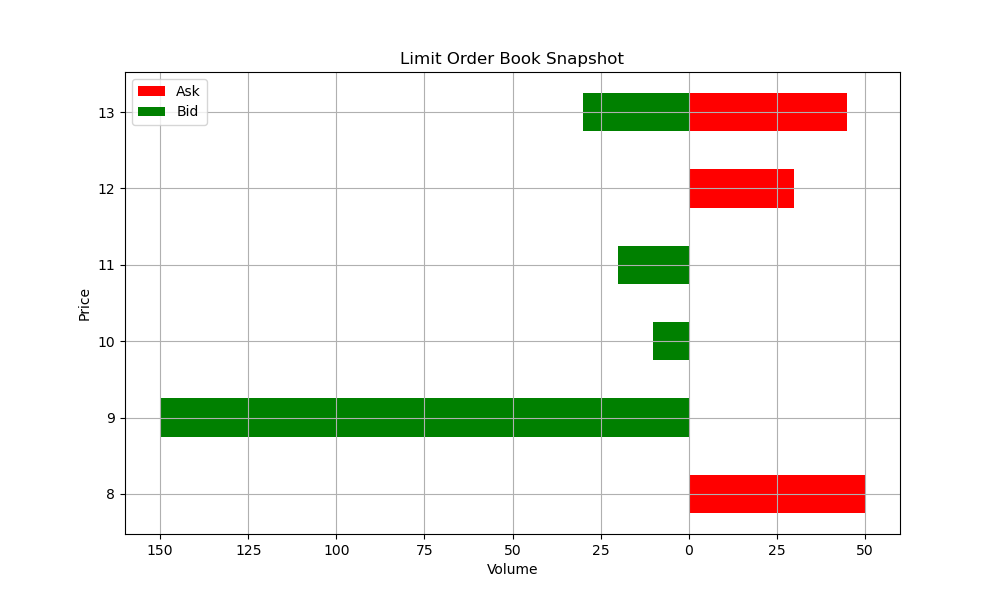
\includegraphics[height=2.5in]{uncleared_example_lob.png}    
    \caption{Aggregated example orders.}
    \label{fig:uncleared_example_orders}
\end{figure}

Following the price-time priority rule, orders 1 through 4 are not marketable and are simply added to the LOB. The aggressive sell order 5 then arrives, clearing orders 1 and 2 entirely and leaving 20 units unexecuted on the ask side sitting at 8 ticks, with the bid side empty. When the buy order 6 arrives, it clears the remaining 20 units of order 5, leaving 130 units on the bid side sitting at 9 ticks. Order 7 next clears 30 units of order 3, leaving 120 units at 12 ticks on the ask side. Another 45 units are then added at price 13 on the ask side. Finally, messages 9 and 10 cancel the remaining volumes of orders 3 and 4. Thus leaving 130 units sitting on the bid side at 9 ticks and 45 units sitting at 13 ticks on the ask side. As a side note, observe that $\mathcal{C}\left( \mathcal{X}(\mathbf{o}) \right) = \left( 150 e_9 + 10 e_{10}, 30 e_{12} + 45 e_{13} \right)$ which is different from the resulting LOB of the example $L(t = 10, \mathbf{o}) = (130 e_9, 45 e_{13})$. This reflects the fact that continuously clearing the LOB (as in trading hours) can yield different results to discrete clearing (as in opening/closing auctions).

Figure~\ref{fig:snapshot_seq} illustrates the corresponding sequence of LOB snapshots resulting from these events.

\begin{figure}[h!]
    \centering
    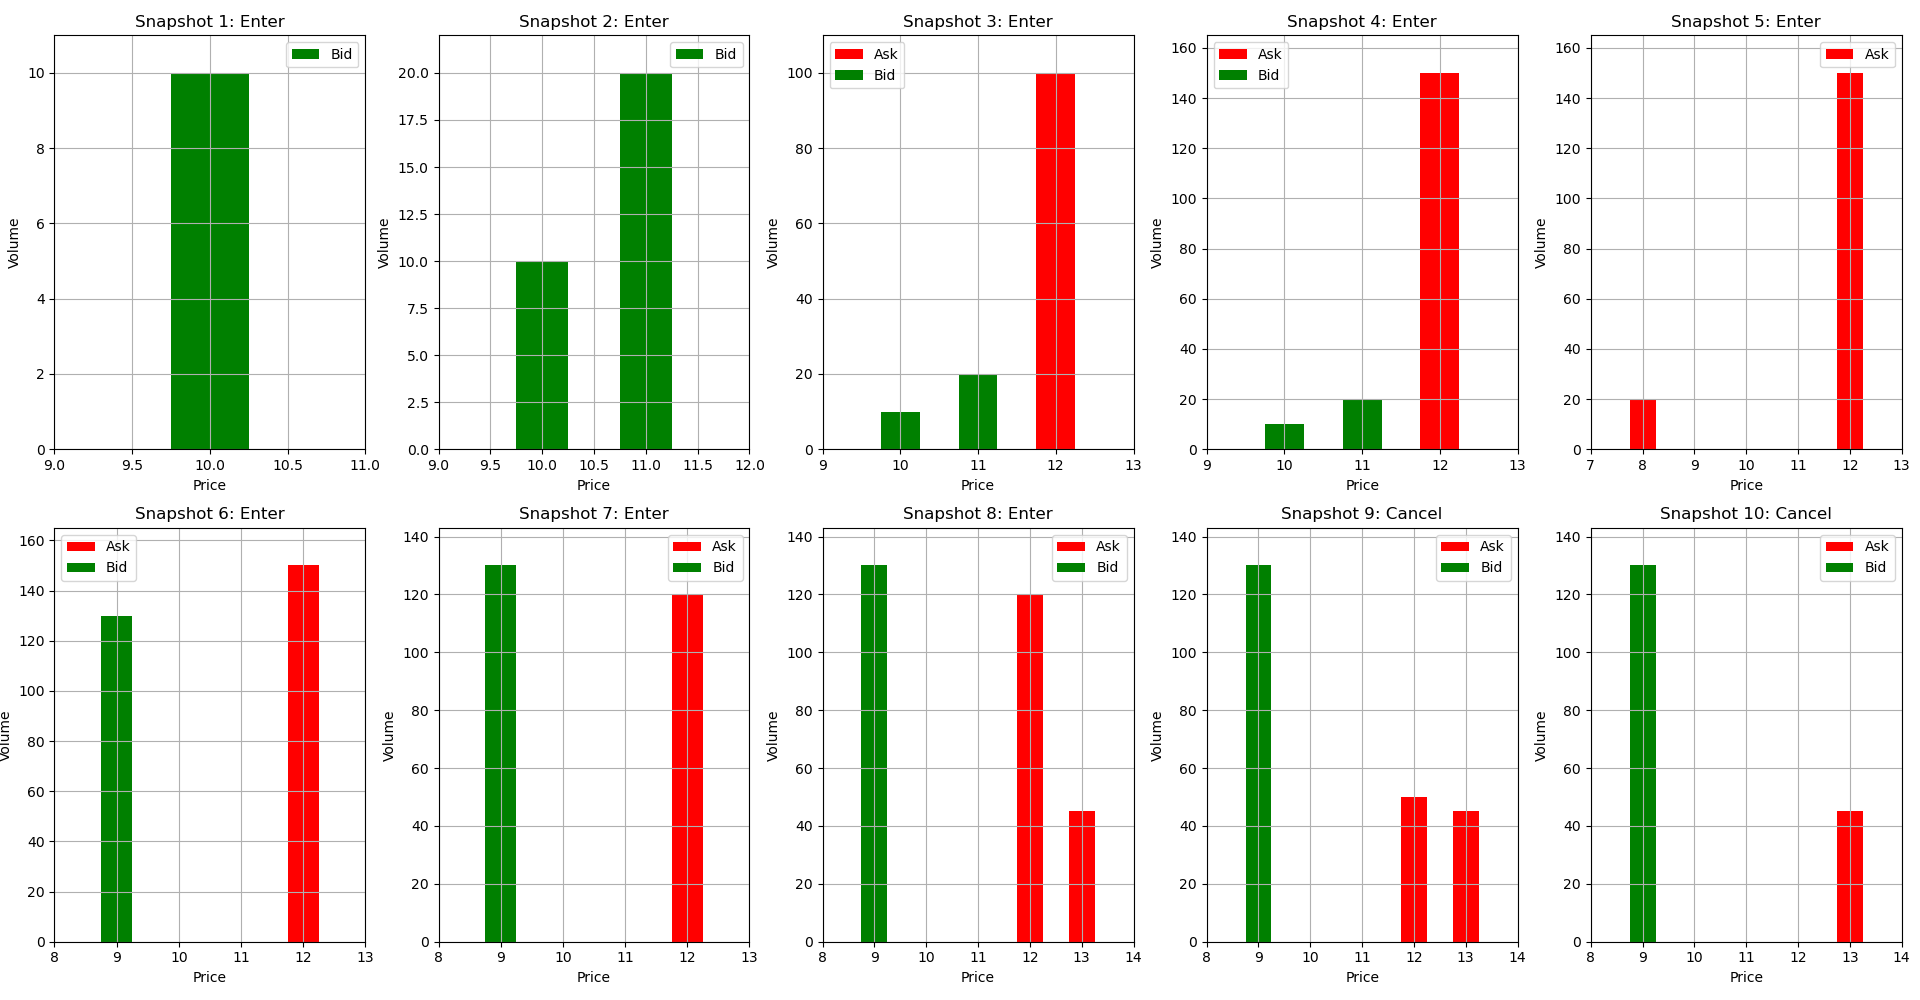
\includegraphics[height=3in]{lob_snapshot_sequence.png}    
    \caption{Sequence of LOB snapshots corresponding to Table \ref{tab:of_example}.}
    \label{fig:snapshot_seq}
\end{figure}

A useful distinction between the OF sequence and MBO data lies in how MBO data can be constructed from the OF sequence without requiring explicit order matching. One way to achieve this is by labeling addition messages as \verb|A| and cancellation messages as \verb|C|. Whenever an outstanding order executes, a series of messages—\verb|T| (trade), \verb|F| (filled), and \verb|C| (cancellation)—can be inserted at the same timestamp to indicate the trade initiator, the filled order, and the final cancellation needed for LOB reconstruction. Under this scheme, the LOB can be fully reconstructed using only \verb|A| and \verb|C| messages, eliminating the need for a separate clearing process. Table \ref{tab:mbo_data} illustrates this procedure.

\begin{table}[H]
  \caption{Example MBO data.}
  \label{tab:mbo_data}

\centering
\scalebox{0.75}{
\begin{tabular}{c c c c c c c}
\hline
\textbf{timestamp} & \textbf{order\_id} & \textbf{side} & \textbf{volume} & \textbf{price} & \textbf{message\_type} \\
\hline
0.04 & 1 & B   & 10  & 10 & A \\
1.23 & 2 & B   & 20  & 11 & A \\
2.45 & 3 & A   & 100 & 12 & A \\
3.14 & 4 & A   & 50  & 12 & A \\
4.75 & 5 & A   & 20  & 11 & T \\
4.75 & 2 & B   & 20  & 11 & F \\
4.75 & 2 & B   & 20  & 11 & C \\
4.75 & 5 & A   & 10  & 10 & T \\
4.75 & 1 & B   & 10  & 10 & F \\
4.75 & 1 & B   & 10  & 10 & C \\
4.75 & 5 & A   & 20  & 8  & A \\
5.63 & 6 & B   & 20  & 8  & T \\
5.63 & 5 & A   & 20  & 8  & F \\
5.63 & 5 & A   & 20  & 8  & C \\
5.63 & 6 & B   & 130 & 9  & A \\
6.14 & 7 & B   & 30  & 12 & T \\
6.14 & 3 & A   & 30  & 12 & F \\
6.14 & 3 & A   & 30  & 12 & C \\
7.85 & 8 & A   & 45  & 13 & A \\
8.32 & 3 & A   & 70  & 12 & C \\
9.78 & 4 & A   & 50  & 12 & C \\
\hline
\end{tabular}}

\end{table}

\clearpage
\section{Alternative Sampling Schemes}
\label{ap:sampling_schemes}
For completeness, we define the \emph{volume bars} partition \(\mathcal{P}^{(V)}\) via the stopping times
\[
\tau^{(V)}_i \;=\;\inf\Bigl\{\,t>\tau^{(V)}_{i-1}:\sum_{k:\,\kappa_k=M}\zeta_k>i\cdot\texttt{Vol}\Bigr\},\quad \tau^{(V)}_0=0,
\]
where \(i,\texttt{Vol}\in\mathbb{Z}^+\). Each interval \(\Delta\tau^{(V)}_i \;=\;\tau^{(V)}_i-\tau^{(V)}_{i-1}\) corresponds to the time required for \(\texttt{Vol}\) units to trade. Furthermore, given any partition \(\mathcal{P}\), we define the counting process
\[
N^{\mathcal{P}}(t)\;=\;\left|\bigl\{\tau\in\mathcal{P}:\,0<\tau\le t\bigr\} \right|,
\]
such that \(N^{\mathcal{P}}(t_1,t_2) = N^{\mathcal{P}}(t_2)-N^{\mathcal{P}}(t_1)\) counts the number of partition points in \((t_1,t_2]\).

\clearpage
\section{CNN–LSTM and DeepLOB Model Specifications}
\label{ap:nn_specs}

This section formalizes the CNN–LSTM and DeepLOB architectures \cite{kolm2023deep, Zhang_2019}.  Section~\ref{subsec:building_blocks} introduces the fundamental tensor operations, which are assembled into the composite layers described in Section~\ref{subsec:composite_structures}.  These composite layers are then connected via convolutional and inception modules to yield the full CNN–LSTM and DeepLOB architectures, as detailed in Section~\ref{subsec:nn_architectures}.

\subsection{Building Blocks}
\label{subsec:building_blocks}

This section describes the fundamental tensor operations that compose the CNN-LSTM and DeepLOB architectures. 

\subsubsection{Permutation}

For simplicity, consider a tensor $T \in \mathbb{R}^{N_1 \times N_2 \times \cdots \times N_d}$ as a multidimensional array with entries denoted by $T_{i_1 i_2 \cdots i_d}$. Denote the data batches as four-dimensional tensors in \(\mathbb{R}^{N \times C \times H \times W}\), where \(N\) denotes the batch size, \(C\) the number of channels, \(H\) the temporal length, and \(W\) the spatial width.

Tensor permutation serves as a higher-dimensional analogue to the matrix transpose. Define the permutation between the $k$-th and $l$-th dimensions as 

\begin{align*}
    \perm^{k, l}: \R^{N_1 \times N_2 \times \cdots \times N_k \times \cdots \times N_l \times \cdots \times N_d} &\rightarrow \R^{N_1 \times N_2 \times \cdots \times N_l \times \cdots \times N_k \times \cdots \times N_d}\\
    T &\mapsto \perm^{k, l}(T)
\end{align*}
where $\bigl[\perm^{k, l}(T)\bigr]_{i_1 i_2 \cdots i_k \cdots i_l \cdots i_d} = T_{i_1 i_2 \cdots i_l \cdots i_k \cdots i_d}$. 

\subsubsection{Concatenation}

Tensor concatenation along the $k$-th dimension is defined as

\begin{align*}
    \concat^k : \mathbb{R}^{N_1 \times N_2 \times \cdots \times N_k \times \cdots \times N_d} \times \mathbb{R}^{N_1 \times N_2 \times \cdots \times N'_k \times \cdots \times N_d} &\rightarrow \R^{N_1 \times N_2 \times \cdots \times (N_k + N'_k) \times \cdots \times N_d}\\
    (T, S) &\mapsto \concat^k(T, S)
\end{align*}
where,

$$
\bigl[\concat^k(T, S)\bigr]_{i_1 i_2  \cdots i_k \cdots i_d} = \begin{cases}
    T_{i_1 i_2 \cdots i_k \cdots i_d} & 1 \leq i_k \leq N_k,\\
    S_{i_1 i_2 \cdots i_k \cdots i_d} & N_k + 1 \leq i_k  \leq N_k + N'_k.
\end{cases}
$$


\subsubsection{Activation Functions}

Two activation functions are necessary: The Sigmoid and the Leaky RelU. For a scalar $x \in \R$ these two activation functions are defined as

\begin{align*}
    \sigmoid(x) &= \frac{1}{1 + \exp(-x)},\\
    \LeakyReLU_{\alpha}(x) &= \begin{cases}
        x & x \geq 0,\\
        \alpha x & x < 0.
    \end{cases}
\end{align*}
For a tensor $T \in \R^{N_1 \times N_2 \times \cdots \times N_d}$, define $\sigmoid: \R^{N_1 \times N_2 \times \cdots \times N_d} \rightarrow \R^{N_1 \times N_2 \times \cdots \times N_d}$  and $\LeakyReLU_{\alpha}: \R^{N_1 \times N_2 \times \cdots \times N_d} \rightarrow \R^{N_1 \times N_2 \times \cdots \times N_d}$

\begin{align*}
    \bigl[\sigmoid(T)\bigr]_{i_1 i_2 \cdots i_d} &= \sigmoid(T_{i_1 i_2 \cdots i_d}),\\
    \bigl[\LeakyReLU_{\alpha}(T)\bigr]_{i_1 i_2 \cdots i_d} &= \LeakyReLU_{\alpha}(T_{i_1 i_2 \cdots i_d}).
\end{align*}

\subsubsection{Batch Normalization}

In the CNN-LSTM model, Spatial Batch Normalization, PyTorch’s \texttt{BatchNorm2d}\footnote{\url{https://pytorch.org/docs/stable/generated/torch.nn.BatchNorm2d.html} (Accessed on 04-29-2025)}, originally proposed in \cite{ioffe2015}, is applied to each convolutional feature map. For a tensor of size $N$ and feature maps of shape $(C,H,W)$, \texttt{BatchNorm2d} computes per-channel statistics over all $N\times H\times W$ activations, then learns one pair of affine parameters $(\gamma_c,\beta_c)$. This normalization is supposed to alleviate the internal covariate shift problem by fixing each channel’s mean to zero and variance to one. This stabilization has been empirically shown to allow for higher learning rates and faster convergence, and can indirectly alleviate issues like vanishing or exploding gradients. 

More precisely, let $T\in\mathbb{R}^{N\times C\times H\times W}$ denote an activation tensor of size $N$ each with $C$ channels of spatial size $H\times W$.  Denote by $T_{icjk}$ the element for sample $i$, channel $c$, and spatial position $(j,k)$. The Spatial Normalization operation is an application $BN^{\phi, \varepsilon} : \R^{N \times C\times H\times W} \rightarrow \R^{N \times C\times H\times W}$ defined as 

\[
\bigl[\batchnorm^{\phi, \varepsilon}(T)\bigr]_{icjk}
= \gamma_c \, \frac{T_{icjk} - \mu_c}{\sqrt{\sigma_c^{2} + \varepsilon}} + \beta_c.
\]
Here, $\gamma_c$ and $\beta_c$ are trainable parameters, $\mu_c$ and $\sigma^2_c$ are channel means and variances respectively, $\phi$ is a momentum hyperparameter and, $\varepsilon$ is a constant used for numerical stability. The computations of $\mu_c$ and $\sigma^2_c$ differ for training and testing. During training, these quantities are computed in a batch-wise fashion as

\[
\mu_c = \mu_c^{(B)} 
= \frac{1}{N\,H\,W}
  \sum_{i=1}^N \sum_{j=1}^H \sum_{k=1}^W
    T_{icjk},
\quad
\sigma_c^{2} = \sigma_c^{2\,(B)} 
= \frac{1}{N\,H\,W}
  \sum_{i=1}^N \sum_{j=1}^H \sum_{k=1}^W
    \bigl(T_{icjk} - \mu_c^{(B)}\bigr)^2.
\]
During testing (or inference) the batch mean, these quantities are computed in the likes of a exponential moving average with momentum $\phi$. That is

\[
\mu_c \leftarrow (1-\phi)\,\mu_c + \phi\,\mu_c^{(B)},
\qquad
\sigma_c^2 \leftarrow (1-\phi)\,\sigma_c^2 + \phi\,\sigma_c^{2\,(B)}.
\]

The interested reader is invited to consult \cite{ioffe2015} for details on the gradients of this transformation and some numerical experiments. 

\subsubsection{Max‐Pooling}

Max‐pooling is a downsampling operation that accentuates the strongest activations within local neighborhoods.  Given a 4D tensor $T \;\in\; \mathbb{R}^{N \times C \times H \times W}$, a max‐pool layer with window size \(n_h \times n_w\) and stride \((s_h,s_w)\) produces an output tensor 
\[
\maxpool^{n_h,n_w}_{s_h,s_w}(T)
\;\in\;
\mathbb{R}^{N \times C \times H' \times W'},
\]
where
\[
H' \;=\;\left\lfloor\frac{H - n_h}{s_h}\right\rfloor + 1,
\quad
W' \;=\;\left\lfloor\frac{W - n_w}{s_w}\right\rfloor + 1.
\]
Its entries are given by
\begin{align*}
    \bigl[\maxpool^{n_h, n_w}_{s_h, s_w}(T)\bigr]_{ickl} = \max \{ T_{ick'l'} :  &k' \in \{ (k - 1) s_h + i' : i' = 1, 2, \dots, n_h \},\\
    &\hspace{10mm} l' \in \{ (l - 1) s_w + j' : j' = 1, 2, \dots, n_w \}\},
\end{align*}
for $i=1,\dots,N$,\; $c=1,\dots,C$,\; $k=1,\dots,H'$,\;
$l=1,\dots,W'$. In other words, each output cell $\left[\maxpool^{n_h, n_w}_{s_h, s_w}(T)\right]_{ickl}$ is the maximum value within the \(n_h\times n_w\) patch of \(T\) starting at spatial location \(((k - 1)\,s_h, (l - 1) \,s_w)\) in channel \(c\) of sample \(i\).


\subsubsection{Zero‐Padding}

Convolution and pooling layers typically reduce spatial dimensions.  However, certain architectures require the output tensor to have the same height and width as the input.  The Zero-padding operation achieves this by surrounding the input with zeros along its spatial axes.  Formally, for $T \;\in\; \mathbb{R}^{N \times C \times H \times W}$, the padded tensor
\[
\zeropad_{p_h,p_w}(T)
\;\in\;
\mathbb{R}^{N \times C \times (H + 2p_h) \times (W + 2p_w)},
\]
has entries
\[
\left[\zeropad_{p_h,p_w}(T)\right]_{ickl}
=
\begin{cases}
0, & k \le p_h \quad\text{or}\quad k > H + p_h,\\[4pt]
0, & l \le p_w \quad\text{or}\quad l > W + p_w,\\[4pt]
T_{ic(k - p_h)(l - p_w)}, & \text{otherwise},
\end{cases},
\]
for \(i=1,\dots,N\), \(c=1,\dots,C\), \(k=1,\dots,H+2p_h\), and \(l=1,\dots,W+2p_w\).  This adds \(p_h\) rows of zeros above and below, and \(p_w\) columns of zeros to the left and right of each feature map.


\subsubsection{Fully Connected Layer}

A fully connected layer performs an affine transformation of its input.  Concretely, given an input vector 
$a \in \mathbb{R}^D$, a weights matrix $W^{(\fullyconnected)}\in \mathbb{R}^{n_h \times D}$, and a bias vector $b \in \mathbb{R}^{n_h}$, the layer output is
\[
\mathrm{FC}_{n_h}(a) \;=\; W^{(\fullyconnected)}\,a \;+\; b
\;\in\; \mathbb{R}^{n_h}.
\]
When applied to a batch of \(N\) inputs, arranged as $A \in \mathbb{R}^{N \times D}$, the same transformation is applied independently to each row:
\[
\bigl[\mathrm{FC}_{n_h}(A)\bigr]_{i \cdot}
\;=\;
\mathrm{FC}_{n_h}\bigl(A_{i \cdot}\bigr),
\quad
i = 1,\dots,N.
\]
Note that $\mathrm{FC}_{n_h}(A) \in \R^{N \times n_h}$

\subsubsection{Convolutional Filters}

Convolutional filters detect local patterns—such as edges or textures—by sliding small learnable kernels over the input.  Concretely, let $T \;\in\; \mathbb{R}^{N \times C \times H \times W}$ and $W^{(\convolution)} \;\in\; \mathbb{R}^{C' \times C \times k_h \times k_w}$ denote, respectively, a batch of \(N\) feature‐map tensors with \(C\) channels and spatial size \(H\times W\), and a set of \(C'\) convolutional kernels of size \(k_h\times k_w\).  With stride \((s_h,s_w)\) and bias vector \(b\in\mathbb{R}^{C'}\), the convolution operation produces the output

$$
\bigl[\convolution^{C', k_h, k_w}_{s_h, s_w}(T)\bigr]_{ic'kl} = \bigl[T * W^{(\convolution)}\bigr]_{ic'kl} + b_{c'},
$$
where
\begin{align*}
    \bigr[T * W^{(\convolution)}\bigl]_{ic'kl} &= \sum^{C}_{c = 1} \sum^{k_h}_{k' = 1} \sum^{k_w}_{l' = 1} T_{ic((k - 1)s_h + k')((l - 1)s_w + l')} W^{(\convolution)}_{c' c k' l'}
\end{align*}
for \(i=1,\dots,N\), \(c'=1,\dots,C'\), \(k=1,\dots,H'\), and \(l=1,\dots,W'\). Note that $\convolution^{C', k_h, k_w}_{s_h, s_w}(T) \in \R^{N \times C' \times H' \times W'}$ where
\[
H' \;=\;\left\lfloor\frac{H - k_h}{s_h}\right\rfloor + 1,
\quad
W' \;=\;\left\lfloor\frac{W - k_w}{s_w}\right\rfloor + 1.
\]
If the stride is \((1,1)\), the subscript may be omitted for notational simplicity.  

\subsubsection{LSTM Layer}

A long–short term memory (LSTM) layer processes sequential inputs while maintaining internal cell and hidden states. Define the LSTM operator \(H_{n_h}\) for input dimension \(D\) and hidden dimension \(n_h\) as follows. For $x \in \mathbb{R}^D,\quad a, c \in \mathbb{R}^{n_h}$, set
\[
H_{n_h}(x,a,c) = (a',c').
\]
Where
\begin{align*}
  \Gamma_f &= \sigmoid\bigl(W^{(fx)}\,x + W^{(fa)}\,a + b^{(f)}\bigr),\\
  \Gamma_u &= \sigmoid\bigl(W^{(ux)}\,x + W^{(ua)}\,a + b^{(u)}\bigr),\\
  \Gamma_o &= \sigmoid\bigl(W^{(ox)}\,x + W^{(oa)}\,a + b^{(o)}\bigr),\\
  \tilde c  &= \tanh\bigl(W^{(cx)}\,x + W^{(ca)}\,a + b^{(c)}\bigr),\\
  c'        &= \Gamma_f \odot c + \Gamma_u \odot \tilde c,\\
  a'        &= \Gamma_o \odot \tanh(c').
\end{align*}
Here, for each gate symbol \(\star\in\{f,u,o,c\}\),
\[
W^{(\star x)}\in\mathbb{R}^{n_h\times D},\quad
W^{(\star a)}\in\mathbb{R}^{n_h\times n_h},\quad
b^{(\star)}\in\mathbb{R}^{n_h},
\]
are trainable parameters, and \(\odot\) denotes element-wise product. Given a sequence $T\in\mathbb{R}^{H\times D}$ with rows \(x^{\langle i\rangle}\) for \(i=1,\dots,H\), initialize
\[
a^{\langle 0\rangle}=0,\quad c^{\langle 0\rangle}=0,
\]
and recursively compute for \(i=1,\dots,H\),
\[
(a^{\langle i\rangle},c^{\langle i\rangle})
= H_{n_h}\bigl(x^{\langle i\rangle},a^{\langle i-1\rangle},c^{\langle i-1\rangle}\bigr).
\]
Define the sequence‑to‑vector transformation
\begin{align*}
    \lstm_{n_h}:\mathbb{R}^{H\times D}&\to\mathbb{R}^{n_h},\\
    T &\mapsto \lstm_{n_h}(T) = a^{\langle H\rangle}.
\end{align*}
For batched input $T\in\mathbb{R}^{N\times H\times D}$, the LSTM acts independently on each batch slice:
\[
\left[\lstm_{n_h}(T)\right]_{i \cdot} = \lstm_{n_h}(T_{i \cdot \cdot}),\quad i=1,\dots,N,
\]
so that
\[
\lstm_{n_h}:\mathbb{R}^{N\times H\times D}\to\mathbb{R}^{N\times n_h}.
\]

\subsection{Composite Structures}
\label{subsec:composite_structures}

\subsubsection{The Composite Convolutional Layer}
\label{subsubsec:comp_conv}

The composite convolutional layer applies three blocks of
\[
  \text{Convolution} \;\to\;\text{LeakyReLU} \;\to\;\text{BatchNorm},
\]
each with its own kernel size and stride. For some input in $\R^{N \times C \times H \times W}$ the composite convolutional layer applies a convolution filter of size $(1, k_w)$ and stride $(1, s_w)$. Observe this filter smooths the features in the space dimension. After applying a Leaky ReLU activation function and Batch Normalization, a time convolution filter of size $(4, 1)$ and stride $(1, 1)$ is applied. Then a Leaky ReLU and Batch Normalization are applied again. This last process is applied twice (see the composite convolution layer in Figure \ref{fig:cnn_lstm_architecture} for a clear representation). Define the outer and inner layers to keep notation compact

\begin{align*}
    \mathrm{Outer}^{k_w}_{s_w}(T) &= \batchnorm^{\phi, \varepsilon} \circ \LeakyReLU_{0.01} \circ \convolution^{32, 1, k_w}_{1, s_w}(T),\\
    \mathrm{Inner}^{(1)}(T) &= \batchnorm^{\phi,\varepsilon}\circ\LeakyReLU_{0.01}\circ\convolution^{32,4,1}(T),\\
\mathrm{Inner}^{(2)}(T) &= \batchnorm^{\phi,\varepsilon}\circ\LeakyReLU_{0.01}\circ\convolution^{32,4,1}(T).
\end{align*}
Thus, the composite convolution layer with initial size $(1, k_w)$ and stride $(1, s_w)$ combines one outer layer and two inner layers as follows 

$$
\mathrm{CConv}^{k_w}_{s_w}(T) = \mathrm{Inner}^{(2)} \circ \mathrm{Inner}^{(1)} \circ \mathrm{Outer}^{k_w}_{s_w} (T).
$$
Unless stated otherwise, no operations within the architecture share trainable parameters.

\subsubsection{The Inception Layer}

The inception layer is used to reduce the amount of computation needed to apply convolution filters in the deeper layers of a neural network \cite{szegedy2015going}. It involves applying a set of $(1, 1)$ sized convolutional filters and max-pooling layers with padding are combined with an activation function and Batch Normalization. Then convolution operations of different size are applied and concatenated. Let us define the following layers

\begin{align*}
    \mathrm{IL}^{(1)}(T) &= \batchnorm^{\phi, \varepsilon, (2)} \circ \LeakyReLU_{0.01} \circ \convolution^{64, 3, 1} \circ ZP^{1,0} \circ \\
    & \hspace{10mm}\batchnorm^{\phi, \varepsilon, (1)} \circ \LeakyReLU_{0.01} \circ \convolution^{64, 1, 1} (T),\\
    \mathrm{IL}^{(2)}(T) &= \batchnorm^{\phi, \varepsilon, (2)} \circ \LeakyReLU_{0.01} \circ \convolution^{64, 5, 1} \circ ZP^{2,0} \circ \\
    & \hspace{10mm} \batchnorm^{\phi, \varepsilon, (1)} \circ \LeakyReLU_{0.01} \circ \convolution^{64, 1, 1} (T), \\
    \mathrm{IL}^{(3)}(T) &= \batchnorm^{\phi, \varepsilon} \circ \LeakyReLU_{0.01} \circ \convolution^{64, 3, 1} \circ MP^{3, 1}_{1, 1} \circ ZP^{1, 0}(T).\\
\end{align*}

Once again, the superscripts in parentheses emphasize that the layers with similar notation do not share trainable parameters. The inception layer is the concatenation, along the second dimension, of these three tensors.

$$
\mathrm{IL}(T) = \concat^{2}(\mathrm{IL}^{(1)}(T), \concat^{2}(\mathrm{IL}^{(2)}(T), \mathrm{IL}^{(3)}(T))).
$$

\subsection{Neural Network Architectures}
\label{subsec:nn_architectures}

\subsubsection{The CNN-LSTM Architecture}
\label{subsubsec:cnn_lstm_architecture}

The CNN-LSTM architecture of Kolm et al. \cite{kolm2023deep}, which is depicted in Figure \ref{fig:cnn_lstm_architecture}, is now formalized. As argued in Section~\ref{subsec:cnn_lstm}, there are multiple possibilities for the neural network output. The multihorizon approach explained this section is considered but the other possibilities can be constructed by modifying the outer layer. Let $K$ be the output dimension. The CNN-LSTM neural network transformation is a map $\cnnlstm : \R^{N \times 100 \times 20} \rightarrow \R^{N \times K}$, where $N$ is the training batch size, defined as

$$
\cnnlstm(\mathbf{X}) = \fullyconnected_K \circ \lstm_{64} \circ \perm^{3, 2} \circ \mathrm{IL} \circ \mathrm{CConv}^{10}_1 \circ \mathrm{CConv}^{2}_2 \left(\mathbf{X}\right).
$$
Here, $\mathbf{X}$ is a 3D tensor of whitened order flow matrices $\widetilde{\mathbf{OF}}^{\mathcal{P}^{(E)}}_{i - 99:i}$. That is,

$$
\mathbf{X} = \left[ \widetilde{\mathbf{OF}}^{\mathcal{P}^{(E)}}_{i_1 - 99:i_1}, \widetilde{\mathbf{OF}}^{\mathcal{P}^{(E)}}_{i_2 - 99:i_2}, \dots, \widetilde{\mathbf{OF}}^{\mathcal{P}^{(E)}}_{i_N - 99:i_N}\right].
$$

Table \ref{tab:cnnlstm} presents the intermediate dimensions of the layers with its respective trainable parameters assuming one horizon ($K = 1$) and a batch of size $32$ ($N = 32$). The resulting model has $133,249$ parameters.


% Please add the following required packages to your document preamble:
% \usepackage{booktabs}
\begin{table}[htb]
  \caption{CNN-LSTM architecture components.}
  \label{tab:cnnlstm}

\centering
\begin{tabular}{@{}lcccc@{}}
\toprule
Layer           & Notation           & Input shape        & Output shape          & Trainable Parameters  \\ \midrule
Conv. Layer     & $\mathrm{CConv}^{2}_2$   & $(32, 1, 100, 20)$ & $(32,  32,  94, 10)$ & 8544           \\
Conv. Layer     & $\mathrm{CConv}^{10}_1$  & $(32, 32, 94, 10)$ & $(32, 32, 88, 1)$    & 18720           \\
Inception Layer & $\mathrm{IL}$            & $(32,  32, 88, 1)$ & $(32, 194, 88, 1)$   & 39872           \\
Permutation     & $\perm^{3,2}$            & $(32, 192, 88, 1)$ & $(32, 88, 192, 1)$   & 0               \\
LSTM            & $\lstm_{64}$             & $(32, 82, 192)$    & $(32, 64)$           & 66048           \\ 
Fully Connected & $\fullyconnected_{1}$    & $(32, 64)$         & $(32, 1)$            & 65   \\\bottomrule
\end{tabular}

\end{table}

During inference mode, the CNN-LSTM architecture will produce an output for each order flow matrix. Such output can be denoted $\cnnlstm \left(\widetilde{\mathbf{OF}}^{\mathcal{P}^{(E)}}_{i - 99:i} \right)$. Moreover, the $\fullyconnected_K$ layer can be bypassed in order to obtain the penultimate layer representation which is effectively a feature map $\phi_{\mathbf{W}} : \R^{100 \times 20} \rightarrow \R^{64}$ defined as

$$
\phi_{\mathbf{W}} \left(\widetilde{\mathbf{OF}}^{\mathcal{P}^{(E)}}_{i - 99:i} \right) =  \lstm_{64} \circ \perm^{3, 2} \circ \mathrm{IL} \circ \mathrm{CConv}^{10}_1 \circ \mathrm{CConv}^{2}_2 \left(\widetilde{\mathbf{OF}}^{\mathcal{P}^{(E)}}_{i - 99:i}\right).
$$
The subscript $\mathbf{W}$ is convenient to highlight the dependency on the parameters of the CNN-LSTM architecture which are updated iteratively.

\begin{figure}[h!]
    \centering
    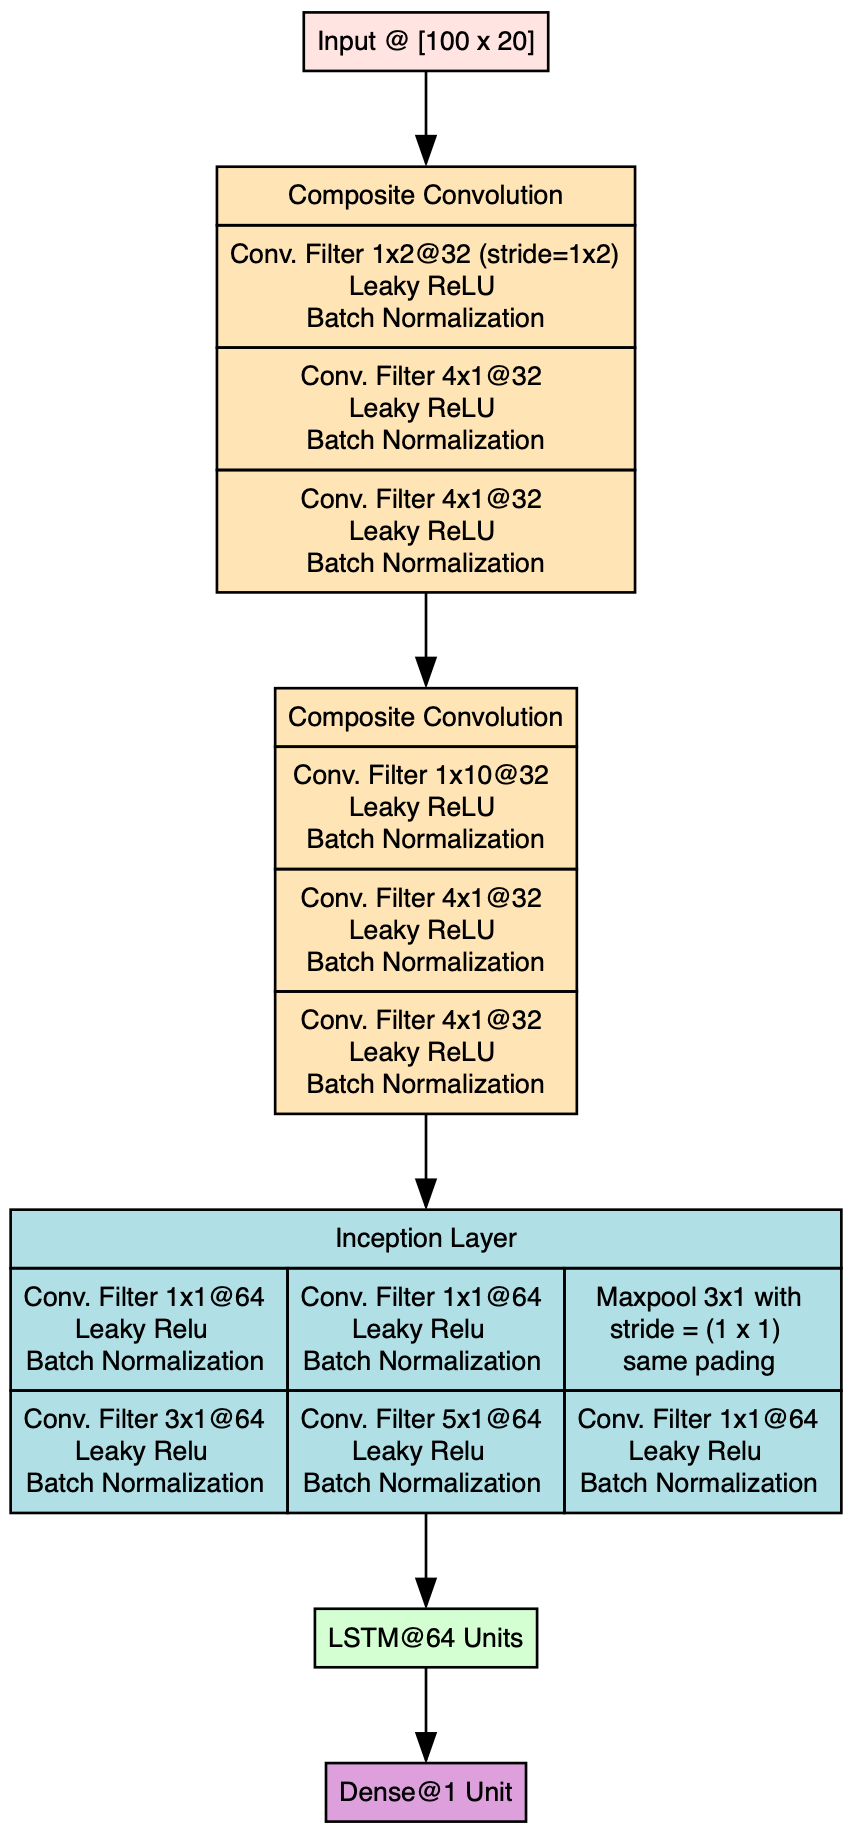
\includegraphics[height=7.5in]{cnn_lstm.png}    
    \caption{Illustration of the CNN-LSTM architecture.}
    \label{fig:cnn_lstm_architecture}
\end{figure}

\subsubsection{The DeepLOB Architecture}

Similarly, the DeepLOB architecture by Zhang et al. \cite{Zhang_2019} adds an extra composite convolutional layer at the top of the CNN-LSTM architecture and takes raw prices and volumes as inputs. Formally $\deeplob : \R^{N \times 100 \times 40} \rightarrow \R^{N \times K}$ with

$$
\deeplob(\mathbf{X}) = \fullyconnected_K \circ \lstm_{64} \circ \perm^{3, 2} \circ \mathrm{IL} \circ \mathrm{CConv}^{10}_1 \circ \mathrm{CConv}^{2, (2)}_2 \circ \mathrm{CConv}^{2, (1)}_2 (\mathbf{X}).
$$
Here, $\mathbf{X}$ is a 3D tensor of whitened limit order book price-volume information as defined in Section~\ref{SubSect:LOB-MBO}:

$$
\mathbf{X} = \left[\tilde{\mathbf{l}}^{\mathcal{P}^{(E)}}_{i_1 - 99 : i_1}, \tilde{\mathbf{l}}^{\mathcal{P}^{(E)}}_{i_2 - 99 : i_2},\dots, \tilde{\mathbf{l}}^{\mathcal{P}^{(E)}}_{i_N - 99 : i_N} \right].
$$

Table \ref{tab:deeplob} illustrates the components of this network assuming a scalar target variable ($K = 1$) and a batch of size 32 ($N = 32$). The resulting model comprises $143,777$ parameters.


% Please add the following required packages to your document preamble:
% \usepackage{booktabs}
\begin{table}[htb]
  \caption{DeepLOB architecture components.}
  \label{tab:deeplob}

\centering
\begin{tabular}{@{}lcccc@{}}
\toprule
Layer           & Notation           & Input shape        & Output shape          & Trainable Parameters  \\ \midrule
Conv. Layer     & $\mathrm{CConv}^{2, (1)}_{2}$ & $(32, 1, 100, 40)$ & $(32, 32, 94, 20)$   & 8544                  \\
Conv. Layer     & $\mathrm{CConv}^{2, (2)}_2$   & $(32, 32, 94, 20)$ & $(32,  32,  88, 10)$ & 10528                 \\
Conv. Layer     & $\mathrm{CConv}^{10}_1$       & $(32, 32, 88, 10)$ & $(32, 32, 82, 1)$    & 18720                 \\
Inception Layer & $\mathrm{IL}$               & $(32,  32, 82, 1)$ & $(32, 194, 82, 1)$   & 39872                 \\
Permutation     & $\perm^{3,2}$        & $(32, 194, 82, 1)$ & $(32, 82, 194, 1)$   & 0                     \\
LSTM            & $\lstm_{64}$        & $(32, 82, 194)$    & $(32, 64)$           & 66048                 \\ 
Fully Connected & $\fullyconnected_{1}$    & $(32, 64)$         & $(32, 1)$            & 65   \\\bottomrule
\end{tabular}

\end{table}



\clearpage
\section{Stationarity Testing}
\label{ap:stationarity_testing}

It is well known in forecasting theory that exogenous variables must be stationary to avoid spurious regressions \cite{xie2006spurious}. Three main tests are adopted:

\noindent \textbf{(A) Augmented Dickey--Fuller (ADF) Test.}
For any variable \(y\) (see Section~\ref{subsec:data_collection}), the ADF test with local trend considers the following autoregressive model:
\[
y_j 
= 
c + \bigl(1 - \phi_1 B - \phi_2 B^2 - \dots - \phi_p B^p\bigr) y_j 
+ 
\varepsilon_j,
\]
which can be equivalently written as
\begin{equation}
\Delta y_j 
= 
\alpha + \gamma y_{j - 1} 
+ 
\sum_{k = 1}^{p - 1} \zeta_k \,\Delta y_{j - k} 
+ 
\varepsilon_j,
\label{eq:adf_autoreg}
\end{equation}
where \(\rho = \sum_{\ell=1}^{p}\phi_\ell\), \(\zeta_k = -\sum_{\ell=k+1}^{p}\phi_\ell\), and \(B\) is the backshift operator. Note that \(\gamma \le 0\), and \(\gamma = 0\) corresponds to \(\rho = 1\), indicating a unit root in \(\phi(z) = 1 - \phi_1 z - \dots - \phi_p z^p\). The ADF test compares
\[
H_0^{\text{ADF}}: \gamma = 0 
\quad \text{versus} \quad
H_1^{\text{ADF}}: \gamma < 0.
\]
Implementation details follow \cite{banerjee1993co} and are available in the \verb|fUnitRoots| package \cite{funitroots2024}. The test statistic is
\[
Z^{\text{ADF}}_t 
= 
\frac{\hat{\gamma}}{\text{s.e.}(\hat{\gamma})},
\]
where \(\hat{\gamma}\) is estimated by ordinary least squares (OLS) on \eqref{eq:adf_autoreg}. Because \(Z^{\text{ADF}}_t\) follows a distribution derived from stochastic integrals rather than a Student’s \(t\)-distribution, the critical values differ accordingly \cite{banerjee1993co}.

A well-known drawback of the ADF test is its sensitivity to the choice of lag length \(p\). In practice, this requires manual input or automated procedures. For simplicity, the current setup fixes \(p = 10\) for all variables. Results from the ADF test are then compared with those of the PP test, which removes the lag-length requirement at the cost of reduced power.

\noindent \textbf{(B) Phillips--Perron (PP) Test.}
The PP test uses a baseline model:
\[
y_j 
= 
\rho\,y_{j - 1} + u_j, 
\quad 
u_j 
= 
\sum_{k=0}^{\infty} \psi_k \,\varepsilon_{j - k} 
= 
\psi(B)\,\varepsilon_j,
\]
where \(\varepsilon_j\) is an iid sequence of random variables with mean zero and variance \(\sigma^2\). Assuming \(\sum_{k=0}^{\infty} k\,\psi_k < \infty\), define 
\(\gamma_k = \mathbb{E}[u_j \,u_{j-k}] = \sigma^2 \sum_{s=0}^{\infty} \psi_s \psi_{s + k}\) and 
\(\lambda = \sigma \sum_{s=0}^{\infty} \psi_s = \sigma\,\psi(1)\). The test contrasts
\[
H_0^{\text{PP}}: \rho = 1 
\quad \text{versus} \quad
H_1^{\text{PP}}: |\rho| < 1.
\]
The statistic is
\[
Z_{\tau}^{\text{PP}} 
= 
\Bigl(\frac{\hat{\gamma}_0}{\hat{\lambda}^2}\Bigr)^{\!1/2}
\frac{\hat{\rho} - 1}{\text{s.e.}(\hat{\rho})}
\;-\;
\frac{1}{2}\Bigl(\hat{\lambda}^2 - \hat{\gamma}_0\Bigr)
\Bigl(\frac{\hat{\lambda}^2}{\sum_{j=1}^{T}(y_j - \bar{y})^2}\Bigr)^{\!1/2},
\]
where 
\begin{align*}
\hat{\gamma}_k 
&= 
\frac{1}{T} \sum_{j=k+1}^{T} \hat{u}_j\,\hat{u}_{j - k},\\
\hat{\lambda}^2 
&= 
\hat{\gamma}_0 
+ 
2 \sum_{k=1}^{q} \Bigl(1 - \frac{k}{q+1}\Bigr)\,\hat{\gamma}_k,\\
q 
&= 
\Bigl\lfloor 12 \Bigl(\frac{T}{100}\Bigr)^{1/4}\Bigr\rfloor.
\end{align*}
Since \(Z_{\tau}^{\text{PP}}\) depends on functionals of Brownian motion rather than standard distributions, critical values must be derived from the appropriate asymptotic theory. This test is implemented via the \verb|urca| package \cite{urca}.

\noindent \textbf{(C) KPSS Test.}
For completeness, the Kwiatkowski--Phillips--Schmidt--Shin (KPSS) test \cite{kwiatkowski1992testing} is included in a confirmatory role. Unlike the ADF and PP tests, the KPSS null hypothesis assumes stationarity. The model is
\[
y_j 
= 
r_j + u_j,
\quad
r_j 
= 
r_{j - 1} + e_j,
\]
where \(e_j\) is an iid sequence with zero mean and variance \(\sigma^2_e\), and \(u_j\) satisfies properties similar to those in the PP framework. That is $u_j = \psi(B) \varepsilon_j$, for some $\varepsilon \overset{iid}{\thicksim} (0, \sigma^2)$, and $\sum^{\infty}_{k = 0} k \psi_k < \infty$. The hypotheses are
\[
H^{KPSS}_0: \sigma_{e}^2 = 0 
\quad\text{versus}\quad 
H^{KPSS}_1: \sigma_{e}^2 > 0.
\]
The test statistic is
\[
\hat{\eta}_{\mu}^{\text{KPSS}} 
= 
\sum_{k=1}^{T} 
\frac{S_k^2}{\hat{\lambda}^2},
\]
where \(S_k = \sum_{j=1}^{k} \hat{u}_j\) represents the partial sum of residuals 
(\(\hat{u}_j = y_j - \bar{y}\)), and \(\hat{\lambda}^2\) follows the same form as in the PP test. As in the previous tests, critical values derive from nonstandard limiting distributions. The \verb|urca| package used for computing the rejection region of the this test.

\clearpage
\section{Case Study: Model Subspace Selection}
\label{ap:case_study_var_selection}

This Monte Carlo study compares adaptive LASSO (adaLASSO) \citep{Zou01122006,MEDEIROS2016255} with OLS-Bonferroni selection for exact support recovery and examines how quickly the failure probability decays to zero. The study is organized as follows. Section~\ref{subsec:background} reviews the Medeiros~\&~Mendes framework describing the DGP and assumptions presented in \cite{MEDEIROS2016255}.  Section~\ref{subsec:simulation_design} describes the particular DGP used for the simulations and the dynamics of design space growth. Section~\ref{subsec:results_and_discussion} analyzes the simulated data to quantify the effect of multicollinearity and initial weights selection. Section~\ref{subsec:conclusions_and_recommendations} draws conclusions and recommendations and Section~\ref{subsec:reproducibility} provides precise instructions for the replication of the present study.

\subsection{Background}
\label{subsec:background}

This section discusses the key regularity conditions and results in \cite{MEDEIROS2016255} and provides some intuitive interpretation to these ideas.

First, consider the data generating process (DGP) 

\begin{equation}
    y_t = \alpha_0 + \boldsymbol{\theta}^T\,\mathbf{x}_t + u_t.
    \label{eq:dgp_medmen}
\end{equation}
Here, $\{\mathbf{x}_t\}_{t \in \Z}$ is an $n_T$-dimensional covariate process, which possibly contains lags of the endogenous process, and $\{u_t\}_{t \in \Z}$ is a martingale difference sequence. Denote by $T$ the sample size of observations of the process $\{y_t \}_{t\in \Z}$, $n_T$ the total number of covariates, and $s_T$ the number of relevant covariates. For simplicity assume that the first $s_T$ elements of $\mathbf{x}_t$ correspond to the relevant variables, which can effectively be denoted as $\mathbf{x}_t = [\mathbf{x}_t(1), \mathbf{x}_t(2)]$. Also write $\boldsymbol{\theta}^T = [\boldsymbol{\theta}^T(1), \boldsymbol{\theta}^T(2)]$ and let $\boldsymbol{\theta}_0$ denote the true parameter which effectively implies that $\boldsymbol{\theta}_0^T = [\boldsymbol{\theta}_0^T(1), \mathbf{0}^T]$. Assuming, without loss of generality, that $\alpha_0 = 0$, The adaLASSO technique consists in minimizing the objective function given by

\[
        f(\boldsymbol{\theta}) = \bigl\|\mathbf{y} -  \mathbf{X}\boldsymbol{\theta}\bigr\|_2^2
        \;+\;\lambda_T\sum_{k} w_k\,|\theta_k|.
\]
Here, $w_k = \left| \theta_{I, k} \right|^{-\tau}$ are computed from $\tau > 0$ and $\boldsymbol{\theta}_I$ an initial parameter estimate. The initial parameter estimate could be given, among others, by OLS, LASSO or elastic-net. The choice of the algorithm for the initial parameters is left out of the scope of this simulation study. Medeiros and Mendes group their assumptions into four categories: Data Generating Process (DGP), Design Space (DESIGN), Initial Weights (WEIGHTS), and Regularization Parameter (REG). These assumptions are restated below for self-completeness.


\begin{itemize}
  \item[(DGP1)] Define $\mathbf{Z}_t = (\mathbf{x}_t^T,\,u_t)^T$. $\{\mathbf{Z}_t\}_{t \in \Z}$ is zero–mean and weakly stationary.
  \item[(DGP2)] $\E \left\{ u_t\mid \SigAl_t\right\}=0$, where $\SigAl_t=\sigma(\mathbf{x}_t, \mathbf{Z}_{t-1}, \mathbf{Z}_{t-2},\dots)$.
  \item[(DGP3)] 
  \[
     \max_{1\le i\le n_T}\Bigl|\tfrac1T\sum_{t=1}^T(x_{it}^2 - E[x_{it}^2])\Bigr|\;\xrightarrow[]{\Prob}0.
  \]
  \item[(DGP4)] For some $m \geq 2$, there exists $c_m < \infty$ such that

  \[
     \E\bigl|x_{it}\,u_t\bigr|^m\;\le c_m \quad \forall t\in \Z, i \in1:n_T.
  \]

  \item[(DESIGN1)] $\mathbf{\theta}_0$ is an open subset $\boldsymbol{\Theta}_{n_T} \subseteq \R^{n_T}$ which contains $\mathbf{0} \in \R^{n_T}$.
  \item[(DESIGN2)] There exists $\theta_{\min} > 0$ such that $\min_{i\le s_T}|\theta_{0,i}|>\theta_{\min}$.
  \item[(DESIGN3)] Denote $\hat{\boldsymbol{\Omega}}_{11} := \frac{1}{T}\mathbf{X}^T(1) \mathbf{X}(1)$ and $\boldsymbol{\Omega}_{11} := \E \left\{ \mathbf{x}_t(1) \mathbf{x}^T_t(1) \right\}$
    \begin{enumerate}
      \item[(a)] There exists a constant $\phi_{\min} \in (0, 1)$ such that
      $$
      \inf_{\norma{\boldsymbol{\alpha}} = 1} \boldsymbol{\alpha}^T \boldsymbol{\Omega}_{11} \boldsymbol{\alpha} > 2 \phi_{\min}.
      $$
      Note that this is equivalent to the smallest eigenvalue of $\boldsymbol{\Omega}_{11}$ being greater than $2\phi_{\min}$.
      \item[(b)] $\norma{\boldsymbol{\Omega}_{11} - \hat{\boldsymbol{\Omega}}_{11}}_{\infty} = \max_{ij} \left| \boldsymbol{\Omega}_{11} - \hat{\boldsymbol{\Omega}}_{11}\right|_{ij} \leq \frac{\phi_{\min}}{s_T}$

    \end{enumerate}

  \item[(WEIGHTS1)] The weights on inactive endogenous variables diverge fast enough: for some $\xi\in(0,1)$ and $c_w>0$,
  \[
    \min_{i \in s_T + 1 : n_T} T^{-\xi/2}\,w_i \;>\; c_w\,\sqrt{\frac{s_T}{\phi_{\min}}},
  \]
  with probability converging to one
  \item[(WEIGHTS2)] The weights on the active set are uniformly bounded: 
  \[
     \sum_{i=1}^{s_T} w_i^2 < s\,w_{\max, T}^2,\quad w_{\max, T}<T^{\xi/2},
  \]
  with probability converging to one.
\end{itemize}

\begin{itemize}
    \item[(REG)] Let $\lambda_T>0$ be the Adaptive‐LASSO penalty parameter.  It is required that
\[
   \frac{n_T^{1/m}T^{(1-\xi)/2}}{\lambda_T}\;\xrightarrow[T \to \infty]{} 0
   \quad\text{and}\quad
   \frac{\lambda_T}{\sqrt{T}}\,\frac{s_T^{1/2}}{w_{\max, T}\,\phi_{\min}}\; \xrightarrow[T \to \infty]{} 0.
\]
\end{itemize}

Further examination of these assumptions reveal interesting patterns. For analysis convenience, define the following dynamics

\begin{align*}
n_T &= \lceil c_{\delta}\,T^{\delta} \rceil, \\[6pt]
s_T &= \lceil c_{\gamma}\,T^{\gamma} \rceil, \\[6pt]
\lambda_T &= c_{\alpha} n_T^{1/m}\;T^{\frac{1-\xi}{2} + \frac{\alpha}{m}}, \\[6pt]
w_{S,T}^2 &= c_{\beta_S}\,T^{\beta_S}, 
\quad
w_{S^c,T}^2 = c_{\beta_{S^c}}\,T^{\beta_{S^c}}.
\\[4pt]
\end{align*}
Here, $w_{S,T}$ and $w_{S^c,T}$ model the growth order of the active and inactive weights respectively. Basic calculus shows that the assumptions (WEIGHTS1), (WEIGHTS2), and (REG) above can be rewritten as

\begin{align*}
\beta_{S^c} - \xi &> \gamma, 
  &&\text{(WEIGHTS1)}\\
\beta_S &< \xi, 
  &&\text{(WEIGHTS2)}\\
\alpha > 0,\quad 
\frac{2}{m}\bigl(\alpha + \delta\bigr) &< \xi - \gamma - \beta_S. 
  &&\text{(REG)}
\end{align*}
These inequalities reveal interesting relationships under the light of the following results.

\begin{theorem}[Theorem 1 of \cite{MEDEIROS2016255}] Under Assumptions \textup{DGP}, \textup{DESIGN}, \textup{WEIGHTS} and \textup{REG}, suppose moreover that
\[
\theta_{\min}
>
\frac{\lambda_T\,s_T^{1/2}}{
  T^{1-\xi/2}\,\phi_{\min}
}.
\]
Then the adaptive LASSO estimator $\hat\theta$ satisfies
\[
\Prob\bigl(\mathrm{sign}(\hat\theta)=\mathrm{sign}(\theta_0)\bigr)
\;\xrightarrow[T \rightarrow \infty]{} 1.
\]
\label{thm:1_medeiros}
\end{theorem}

In the theorem above, the $\mathrm{sign}$ function is defined as $\mathrm{sign}(x) = I_{\{ x > 0 \}} - I_{\{ x < 0 \}}$ which implies that $\mathrm{sign}(0) = 0$.

\begin{theorem}[Theorem 2 of \cite{MEDEIROS2016255}] Let $\hat{\boldsymbol{\theta}}_{\text{ols}}{(1)}$ denote the OLS estimator of the true active coefficients $\boldsymbol{\theta}_0{(1)}$.  Under the assumptions of Theorem~\ref{thm:1_medeiros}, it holds that for any $s_T$‑vector $\boldsymbol{\alpha}$ with $\|\boldsymbol{\alpha}\|_2=1$,
\[
\sqrt{T}\,\boldsymbol{\alpha}^T\,\bigl(\hat{\boldsymbol{\theta}}{(1)} - \boldsymbol{\theta}_0{(1)}\bigr)
=
\sqrt{T}\,\boldsymbol{\alpha}^T\,\bigl(\hat{\boldsymbol{\theta}}_{\text{ols}}{(1)} - \boldsymbol{\theta}_0{(1)}\bigr)
\;+\;o_p(1).
\]
\end{theorem}

Theorem 2—often called the \textit{oracle property}—goes one step further: not only does the adaptive LASSO select the correct support with probability tending to one, but its active‐set estimates are asymptotically as efficient as if we knew the true model in advance. Moreover, the proof of Theorem 1 shows that, for some $c>0$ and for a sufficiently large \(T\),
\begin{equation}
\Prob\bigl(\mathrm{sign}(\hat\theta)\neq\mathrm{sign}(\theta_0)\bigr)
\;\le\;
\frac{c}{T^\alpha},
\label{eq:decay_rate}
\end{equation}
so the probability of selection failure decays at rate \(T^{-\alpha}\). In practice this means that larger \(\alpha\) yields faster convergence—yet \(\alpha\) itself is bounded by the REG assumption’s \textit{window}. Note also that heavier‐tailed errors (smaller \(m\)) tighten this window, as do steeper growth in the number of covariates, denser true parameter vectors \(\theta_0\), or more aggressive penalization on the active set.

\subsection{Simulation Design}
\label{subsec:simulation_design}


Simulated data is generated from the DGP

\begin{equation*}
y_t 
= 
\displaystyle \phi y_{t - 1}
\;+\;
\sum^{n_T}_{j = 1} \beta_j\,x_{j t}
\;+\; u_t,  
\end{equation*}
where,

\[
\begin{cases}
\mathbf{x}_t=
\displaystyle \phi_X \,\mathbf{x}_{t-1}
\;+\;
\mathbf{L}\,\mathbf{v}_t,
&
v_{jt} \overset{iid}{\sim} t_{m + 1},\\[2ex]
u_t = \sigma_t \eta_t 
&
\eta_t \overset{iid}{\sim} t_{m + 1},\\[2ex]
\sigma^2_t = \omega + \alpha_{\star} u_{t - 1}^2 + \beta_{\star} \sigma^2_{t - 1}.
\end{cases}.
\]
Here, $\phi_X$ is a scalar and $\mathbf{L}$ is chosen to be a lower triangular matrix such that $\mathbf{R} := \mathbf{L} \mathbf{L^T}$, where $\mathbf{R}$ is the desired correlation matrix. Take $\beta_j = 1$ if $j \leq s_T$ and zero otherwise. Take $\phi = 0.8$, $\phi_X = 0.5$, $\omega = 0.1$, $\alpha_\star = 0.1$, $\beta_\star = 0.8$, and $m = 8$. Construct $\mathbf{R}$ starting from the identity matrix and replace its entries $(1, 2)$ and $(2, 1)$ with $\rho$ (i.e. $\mathbf{R}_{1,2} = \mathbf{R}_{2,1} = \rho$), where $\rho \in \{0, 0.25, 0.5, 0.75, 0.99 \}$. The parameters governing the dynamics of the number of candidate variables and penalizing weights are given below.


\begin{table}[h]
  \caption{Simulation parameters.}

\centering
\begin{tabular}{ccccccccccc}
\hline
$c_{\alpha}$ & $\alpha$ & $c_{\beta_{S}}$ & $\beta_{S}$ & $c_{\beta_{S^c}}$ & $\beta_{S^c}$ & $c_{\gamma}$ & $\gamma$ & $c_{\delta}$ & $\delta$ & $\xi$ \\
\hline
1 & 0.25 & 1 & 0.125 & 1 & 1.5 & 2 & 0.25 & 1 & 0.5 & 0.75 \\
\hline
\end{tabular}

\end{table}

Partitioning the interval $[64,1024]$ into 15 roughly equally‐spaced values of $T$ produces the simulation grid shown in Table~\ref{tab:simulation_grid}.  Each $(T,n_T,s_T)$ configuration is then replicated $N=100$ times for each of the specified correlation levels. For each of the samples, adaLASSO is fit assuming equal weights for the active set ($w_{S,T}$) and weights equal to $w_{S^c, T}$ for the inactive set. This helps to control the dynamics of the penalizing weights which in practice emerge from $\tau$ and the initial estimate selection algorithm. For simplicity, the weight corresponding to the lagged value of $y_t$ is left close to zero and only one lag is included in $\mathbf{X}$. OLS is then fit and the variance of $\hat{\tilde{\boldsymbol{\beta}}}$ is estimated via the homoskedastic formula (as a benchmark) and the heteroskedasticity-consistent estimator (HCE). Specifically

\begin{align*}
    \hat{V}_{\mathrm{hom}} &= \hat{\sigma}^2(\tilde{\boldsymbol{X}}^T \tilde{\boldsymbol{X}})^{-1}; \quad  \hat{\sigma}^2 = \frac{1}{T - n_T - 1}\sum^{T}_{t = 1} \hat{u}_t^2,\\
    \hat{V}_{\mathrm{het}} &= (\tilde{\boldsymbol{X}}^T \tilde{\boldsymbol{X}})^{-1} \left( \sum^T_{t = 1} \tilde{\mathbf{x}}_t \tilde{\mathbf{x}}^T_t \hat{u}^2_t \right) (\tilde{\boldsymbol{X}}^T \tilde{\boldsymbol{X}})^{-1},
\end{align*}
where in the above the \textit{tilded} quantities denote the corresponding augmented quantity to account for the inclusion of one lag of the endogenous variable. Statistical significance is assessed throught the $t$ test with Bonferroni correction. That is, a variable will be selected following each of the OLS approaches iff

\begin{align*}
    \frac{\hat{\tilde{\beta}}_i}{V_{ii}^{1 / 2}} > t_{T - s_T - 1, 1 - \frac{0.025}{(n_T + 1)}}.
\end{align*}
Following the execution of these three variable selection algorithms. The proportion of correctly selected models is calculated for each of the different $T \rho$-combinations.


\begin{table}[ht]
  \caption{Simulation grid: sample size $T$ and corresponding $n_{T}=\lceil c_{\delta} T^{\delta}\rceil$, $s_{T}=\lceil c_{\gamma}T^{\gamma}\rceil$.}
  \label{tab:simulation_grid}

\centering
\begin{tabular}{ccc}
\toprule
$T$   & $n_{T}$ & $s_{T}$ \\
\midrule
64    &  8  &  6  \\
133   & 12  &  7  \\
202   & 15  &  8  \\
270   & 17  &  9  \\
339   & 19  &  9  \\
407   & 21  &  9  \\
476   & 22  & 10  \\
544   & 24  & 10  \\
613   & 25  & 10  \\
682   & 27  & 11  \\
750   & 28  & 11  \\
819   & 29  & 11  \\
887   & 30  & 11  \\
956   & 31  & 12  \\
1024  & 32  & 12  \\
\bottomrule
\end{tabular}

\end{table}




\subsection{Results and Discussion}
\label{subsec:results_and_discussion}

\subsubsection{Multicollinearity Effect}

Figure~\ref{fig:exact_recovery_corr} (see Section \ref{sec:comp_tables_figs}) displays the exact recovery rate (fraction of simulations where $\mathrm{sign}(\hat{\boldsymbol{\theta}}) = \mathrm{sign}(\boldsymbol{\theta})$) as a function of $T$, for different correlation levels $\rho$. Several clear patterns emerge. First, as expected, increasing the sample size improves support recovery for both methods in all scenarios – the curves generally rise toward 1.0 as $T$ grows. However, the adaLASSO (red curves) achieves much higher recovery rates at moderate sample sizes than OLS (blue/green curves) in the presence of strong multicollinearity. For low correlation ($\rho=0$ or $0.25$), the gap between methods is small: OLS with Bonferroni performs nearly as well as adaLASSO when predictors are independent or only mildly correlated. In fact, for $\rho=0$, both methods eventually reach ~100\% recovery with sufficiently large $T$ (hundreds of observations), and their trajectories are quite close. This is because when predictors are uncorrelated, the OLS t-tests remain informative (each coefficient can be estimated independently with little variance inflation), so the Bonferroni penalty for multiple testing is the main hurdle – which large $T$ can overcome by reducing standard error. AdaLASSO also works well in this regime, effectively similar to the ordinary LASSO which is known to be consistent under mutual independence of features.

When correlation increases to moderate levels ($\rho=0.5$ shown in Figure \ref{fig:exact_recovery_corr}, top-right panel, and $\rho=0.75$ in bottom-left), the performance of OLS selection deteriorates dramatically relative to adaLASSO. For $\rho=0.5$, the OLS method (blue/green lines) requires a much larger $T$ to approach high recovery probability – there is a noticeable rightward shift of the OLS curve compared to the adaLASSO curve. The adaLASSO achieves near-perfect support recovery at $T = 339$ observations when $\rho=0.5$, whereas OLS-Bonferroni needs roughly double that sample size to reach comparable accuracy. The gap widens further at $\rho=0.75$: here the OLS approach almost never succeeds for small or moderate samples (recovery probability essentially 0 for $T < 300$). Even at $T = 1024$, OLS is only recovering the true model in about 50–60\% of trials, whereas adaLASSO already exceeds 90\% success by that point.  the adaLASSO appears more robust to multicollinearity when $T$ is large enough, eventually achieving near-certain recovery even at $\rho=0.75$ in the simulations (red curve tending to 1.0 as $T$ grows). OLS, however, remains very sensitive: even at $T=1024$, the OLS method never reaches 100\% recovery for $\rho=0.75$.

The most extreme case is $\rho=0.99$ (Figure~\ref{fig:exact_recovery_corr}, bottom-middle), where predictors are almost perfectly correlated. This scenario is akin to having duplicate or nearly-duplicate variables in the dataset – a problem for OLS inference. Accordingly, the OLS selection method essentially fails entirely: the blue/green curves at $\rho=0.99$ sit near zero across all sample sizes tested. The adaLASSO (red curve) also finds this scenario challenging (its recovery probability grows only slowly with $T$ and does not reach 1 even at $T = 1024$), but it clearly outperforms OLS: by $T = 1024$ observations, adaLASSO achieves about 70\% exact recovery, whereas OLS is essentially at 0\%. This sensitivity to multicollinearity of the adaLASSO approach connects with the assumption DESIGN3 as $\phi_{\mathrm{min}}$ decreases with $\rho$. The simulation confirms that multicollinearity breaks down the performance of naive OLS variable selection, while adaLASSO is far more resilient in discovering the correct predictors (especially as $T$ becomes large).

To connect with the theoretical result from \cite{MEDEIROS2016255} (see \ref{eq:decay_rate}), the rate at which the failure probability decreases with $T$ is examined. Figure~\ref{fig:log_log_failure_rate_corr} plots the Monte Carlo estimated failure rates on logarithmic scales. If the failure probability follows a power-law $T^{-\alpha}$, an approximately straight line with slope $-\alpha$ in the log–log representation would be observed. Indeed, for the adaLASSO (red) a roughly linear downward trend in all panels is seen - except when the curve saturates -, consistent with a polynomial decay in $T$. At every correlation level, the estimated failure rate (red) declines faster than the theoretical bound line (dashed), indicating a steeper power‑law exponent. Thus, the adaLASSO simulation results are consistent with the theoretical guarantee of polynomial-decay consistency: even under dependence and heavy-tailed noise, it is observed that $\Prob\bigl(\mathrm{sign}(\hat\theta)\neq\mathrm{sign}(\theta_0)\bigr)$ trends down at least as fast as $c T^{-\alpha}$ for some $\alpha>0$.

The OLS-based methods (blue/green lines in Figure \ref{fig:log_log_failure_rate_corr}) tell a similar story when the multicollinearity level is below or at 50\%. However, the failure probability rate of decrease exhibits a slower convergence when the multicollinearity level is at or above 75\%. This reflects the fact that OLS with Bonferroni can eventually consistently select the true model when predictors have low to moderate correlation. For higher correlations ($\rho \geq 0.75$), the blue/green points in Figure \ref{fig:log_log_failure_rate_corr} are almost horizontal or very mildly declining on the log–log scale. This underscores the superior performance of adaLASSO under high multicollinearity regimes when the DGP, DESIGN, WEIGHTS, and REG conditions hold.

\subsubsection{Effect of Initial Weights}

It might be suggested that adaLASSO may enjoy an unfair edge under the simulation configuration presented, since the true parameter values are “encoded” in the evolution of the penalty weights \(w_i\). To address this concern, a targeted sensitivity experiment was conducted: setting the correlation parameter \(\rho=0\) and raising the inactive‐set weights to \(\beta_{S^c}=1.15\), while holding all other hyper‐parameters fixed. The results (Figures~\ref{fig:exact_recovery_beta} and~\ref{fig:log_log_failure_rate_beta}) show that, under these conditions, adaptive‐LASSO requires substantially larger sample sizes before its exact‐recovery probability saturates. Crucially, however, once the sample size exceeds a threshold, the failure probability decays very rapidly, in line with the oracle‐type behavior predicted by theory.

These findings make clear that careful tuning of the initial‐weight construction is important when \(T\) is limited or the signal in the inactive set is relatively strong.

\subsection{Conclusions and Recommendations}
\label{subsec:conclusions_and_recommendations}

In this Monte Carlo case study the adaLASSO and Bonferroni-corrected t-tests were compared, focusing on exact support recovery and the empirical rate at which the failure probability decays to zero.  The main findings are:

\begin{itemize}
  \item \textbf{Exact recovery vs.\ multicollinearity.}  When predictors are uncorrelated or only mildly correlated ($\rho\le0.25$), both methods eventually recover the true support with high probability as $T$ grows.  However, under moderate to strong multicollinearity ($\rho\ge0.5$), OLS-Bonferroni requires much larger $T$ and in extreme cases ($\rho=0.99$) essentially fails, whereas adaLASSO still achieves a decent recovery rate for moderately large samples.
  \item \textbf{Polynomial decay of failure rate.}  On a log–log scale, the adaLASSO’s failure probability exhibits an approximately linear decline of slope $-\alpha$, consistent with the theoretical bound
  \[
    \Pr\bigl(\mathrm{sign}(\hat\theta)\neq\mathrm{sign}(\theta_0)\bigr)\;\lesssim\;c\,T^{-\alpha}.
  \]
  In contrast, OLS-Bonferroni only attains an adaLASSO-comparable decay when $\rho$ is small; its curve flattens out for higher correlations.
  \item \textbf{Sensitivity to initial‐weight tuning.}  By increasing the inactive‐set exponent $\beta_{S^c}$, it was shown that adaLASSO may require larger $T$ before its recovery probability ``saturates.''  Yet once past a moderate threshold, its convergence is very rapid, demonstrating the oracle‐property in practice. This underscores the importance of the selection of an initial weights selection method that discriminates inactive variables.
\end{itemize}

\noindent
\textbf{Practical recommendations.}  Based on these results, practitioners should:
\begin{itemize}
  \item Employ adaLASSO in high‐dimensional, time‐series settings where multicollinearity is present, since it substantially outperforms OLS‐based selection under dependence.
  \item Carefully tune the hyperparameters of the initial weights selection.
  \item Use OLS-Bonferroni as a simple baseline when predictors are mildly correlated.
  \item Validate selection performance before deploying the method in empirical applications.
\end{itemize}

\noindent
Overall, the present study confirms that adaLASSO not only achieves model selection consistency and the oracle property under the Medeiros \& Mendes framework, but also delivers robust performance in finite samples—especially when multicollinearity and heteroskedastic, heavy‐tailed errors are present.

\subsection{Reproducibility}
\label{subsec:reproducibility}

All the simulation results presented here can be reproduced using the code available in the GitHub repository \url{judmejiabe/case-study-adaLASSO}. The repository contains detailed scripts for generating the data, running the adaptive LASSO and OLS selection procedures, and producing the figures.

\clearpage
\section{Events Matching Exclusion Criteria on the INTC MBO Dataset}
\label{sec:exclusion_criteria}

This section lists the dates excluded from the analysis as a consequence of meeting any of the excluding criteria highlighted in Section~\ref{subsec:dataset}. The exclusion criteria is reproduced below for the reader's convenience.

\begin{itemize}
    \item Corporate actions: Ex-dividend dates, stock splits or reverse splits, share buybacks and rights issues, spin-offs, mergers, or acquisitions
    \item Earnings and company-specific news: Quarterly earnings announcements and guidance revisions, joint ventures, large partnerships or asset sales, regulatory actions or class-action lawsuits, product launches or major technological disclosures
    \item Derivative market events: Monthly options expirations (OPEX), quarterly triple witching weeks (stock index futures, index options, and single-stock options expiry), index futures rollovers (e.g., NASDAQ-100, S\&P 500), index and ETF quarterly rebalancing
    \item Scheduled announcements: U.S. Employment Situation (non-farm payrolls), Consumer Price Index (CPI), Producer Price Index (PPI), PCE releases, FOMC interest rate decisions and press conferences, other major macroeconomic indicators (e.g., GDP, JOLTS)
    \item Exchange halts: Limit-Up/Limit-Down (LULD) volatility pauses, market-wide circuit breakers, exchange-initiated suspensions (technical or regulatory).
\end{itemize}

\subsection{Corporate Actions}

\begin{itemize}
    \item May 6, 2024. Event Type: Ex-dividend date. Description: Ex-dividend date for quarterly cash dividend of \$0.125 per share. Source: \url{https://stocklytics.com/stocks/intc/dividends}
\end{itemize}

\subsection{Earnings and Company-Specific News}

\begin{itemize}
    \item April 25, 2024 (after market close, impacting May 1). Event Type: Earnings release. Description: Intel reported Q1 2024 earnings, the first quarter under its internal foundry reporting model; the Foundry segment revenue was \$4.4 billion (down 10\% year-over-year). Source: \url{https://www.intc.com/news-events/press-releases/detail/1635/intel-reports-first-quarter-2024-financial-results}
    \item May 8, 2024. Event Type: Regulatory action (export license revocation). Description: The U.S. Commerce Department revoked certain export licenses for shipments to Huawei, affecting Intel's ability to supply that customer. Source: \url{https://www.marketwatch.com/story/intels-stock-drops-after-u-s-revokes-licenses-for-exports-to-china-customer-f057da21}
    \item June 4, 2024. Event Type: Joint venture. Description: Intel and Apollo announced a definitive agreement under which Apollo acquired a 49\% equity stake in a joint venture related to Intel's Fab 34 facility in Leixlip, Ireland (Intel retains operational control). Source: \url{https://newsroom.intel.com/corporate/co-invest-program-news-2024}
    \item June 17, 2024. Event Type: Class action lawsuit. Description: Bronstein, Gewirtz \& Grossman announced a securities-fraud class action against Intel regarding statements about the internal foundry model and foundry losses (class period Jan 25--Apr 25, 2024). Source: \url{https://www.globenewswire.com/de/news-release/2024/05/13/2880132/0/en/INTC-INVESTOR-ALERT-Bronstein-Gewirtz-Grossman-LLC-Announces-that-Intel-Corporation-Investors-with-Substantial-Losses-Have-Opportunity-to-Lead-Class-Action-Lawsuit.html}
    \item June 21, 2024. Event Type: Class action lawsuit notice. Description: Levi \& Korsinsky announced a class action filing and lead-plaintiff deadline of July 2, 2024, reiterating allegations concerning Intel's internal foundry disclosures. Source: \url{https://www.prnewswire.com/news-releases/class-action-filed-against-intel-corporation-intc---july-2-2024-deadline-to-join--contact-levi--korsinsky-302178578.html}
\end{itemize}

\subsection{Derivative Market Events}

\begin{itemize}
    \item May 17, 2024. Event Type: Options expiration (OPEX). Description: Monthly U.S. equity and ETF options expiration. Source: \url{https://www.macroption.com/options-expiration-calendar/}
    \item June 17-21, 2024. Event Type: Triple witching week. Description: Simultaneous expiration of stock index futures, stock index options, and single-stock options, coinciding with June OPEX. Source: \url{https://www.bankrate.com/investing/triple-witching/}
\end{itemize}

\subsection{Scheduled Announcements}

\begin{itemize}
    \item May 3, 2024. Event Type: U.S. Employment Situation (April NFP). Description: BLS reported non-farm payrolls at 175k (below consensus), released at 8:30a ET. Source: \url{https://www.bls.gov/news.release/archives/empsit_05032024.htm}
    \item May 15, 2024. Event Type: CPI release (April). Description: Consumer Price Index data released at 8:30a ET. Source: \url{https://www.bls.gov/news.release/archives/cpi_05152024.htm}
    \item June 4, 2024. Event Type: JOLTS (Job Openings). Description: The Bureau of Labor Statistics released the April Job Openings and Labor Turnover Survey at 10:00 a.m. ET. Source: \url{https://www.bls.gov/news.release/archives/jolts_06042024.htm}
    \item June 7, 2024. Event Type: U.S. Employment Situation (May NFP). Description: Non-farm payrolls release at 8:30a ET. Source: \url{https://www.bls.gov/news.release/archives/empsit_06072024.htm}
    \item June 12, 2024. Event Type: CPI release (May). Description: Consumer Price Index release at 8:30a ET. Source: \url{https://www.bls.gov/news.release/archives/cpi_06122024.htm}
    \item June 12, 2024. Event Type: FOMC decision. Description: Federal Reserve announced policy decision and released updated Summary of Economic Projections at 2:00p ET, followed by press conference. Source: \url{https://www.federalreserve.gov/monetarypolicy/fomccalendars.htm}
    \item June 13, 2024. Event Type: PPI release (May). Description: Producer Price Index release at 8:30a ET. Source: \url{https://www.bls.gov/news.release/archives/ppi_06132024.htm}
    \item June 14, 2024. Event Type: Import/Export Prices (May). Description: BLS Import and Export Price Indexes released at 8:30a ET. Source: \url{https://www.bls.gov/news.release/archives/ximpim_06142024.htm}
\end{itemize}

\subsection{Exchange Halts}

\begin{itemize}
    \item None. No Nasdaq trading halts were recorded for INTC between May 1 and June 30, 2024. Source: Nasdaq Trader Trading Halts database \url{https://www.nasdaqtrader.com/Trader.aspx?id=TradeHalts}
\end{itemize}

\clearpage
\section{Complimentary Tables and Figures}
\label{sec:comp_tables_figs}

\begin{sidewaysfigure}[htb]
    \centering
    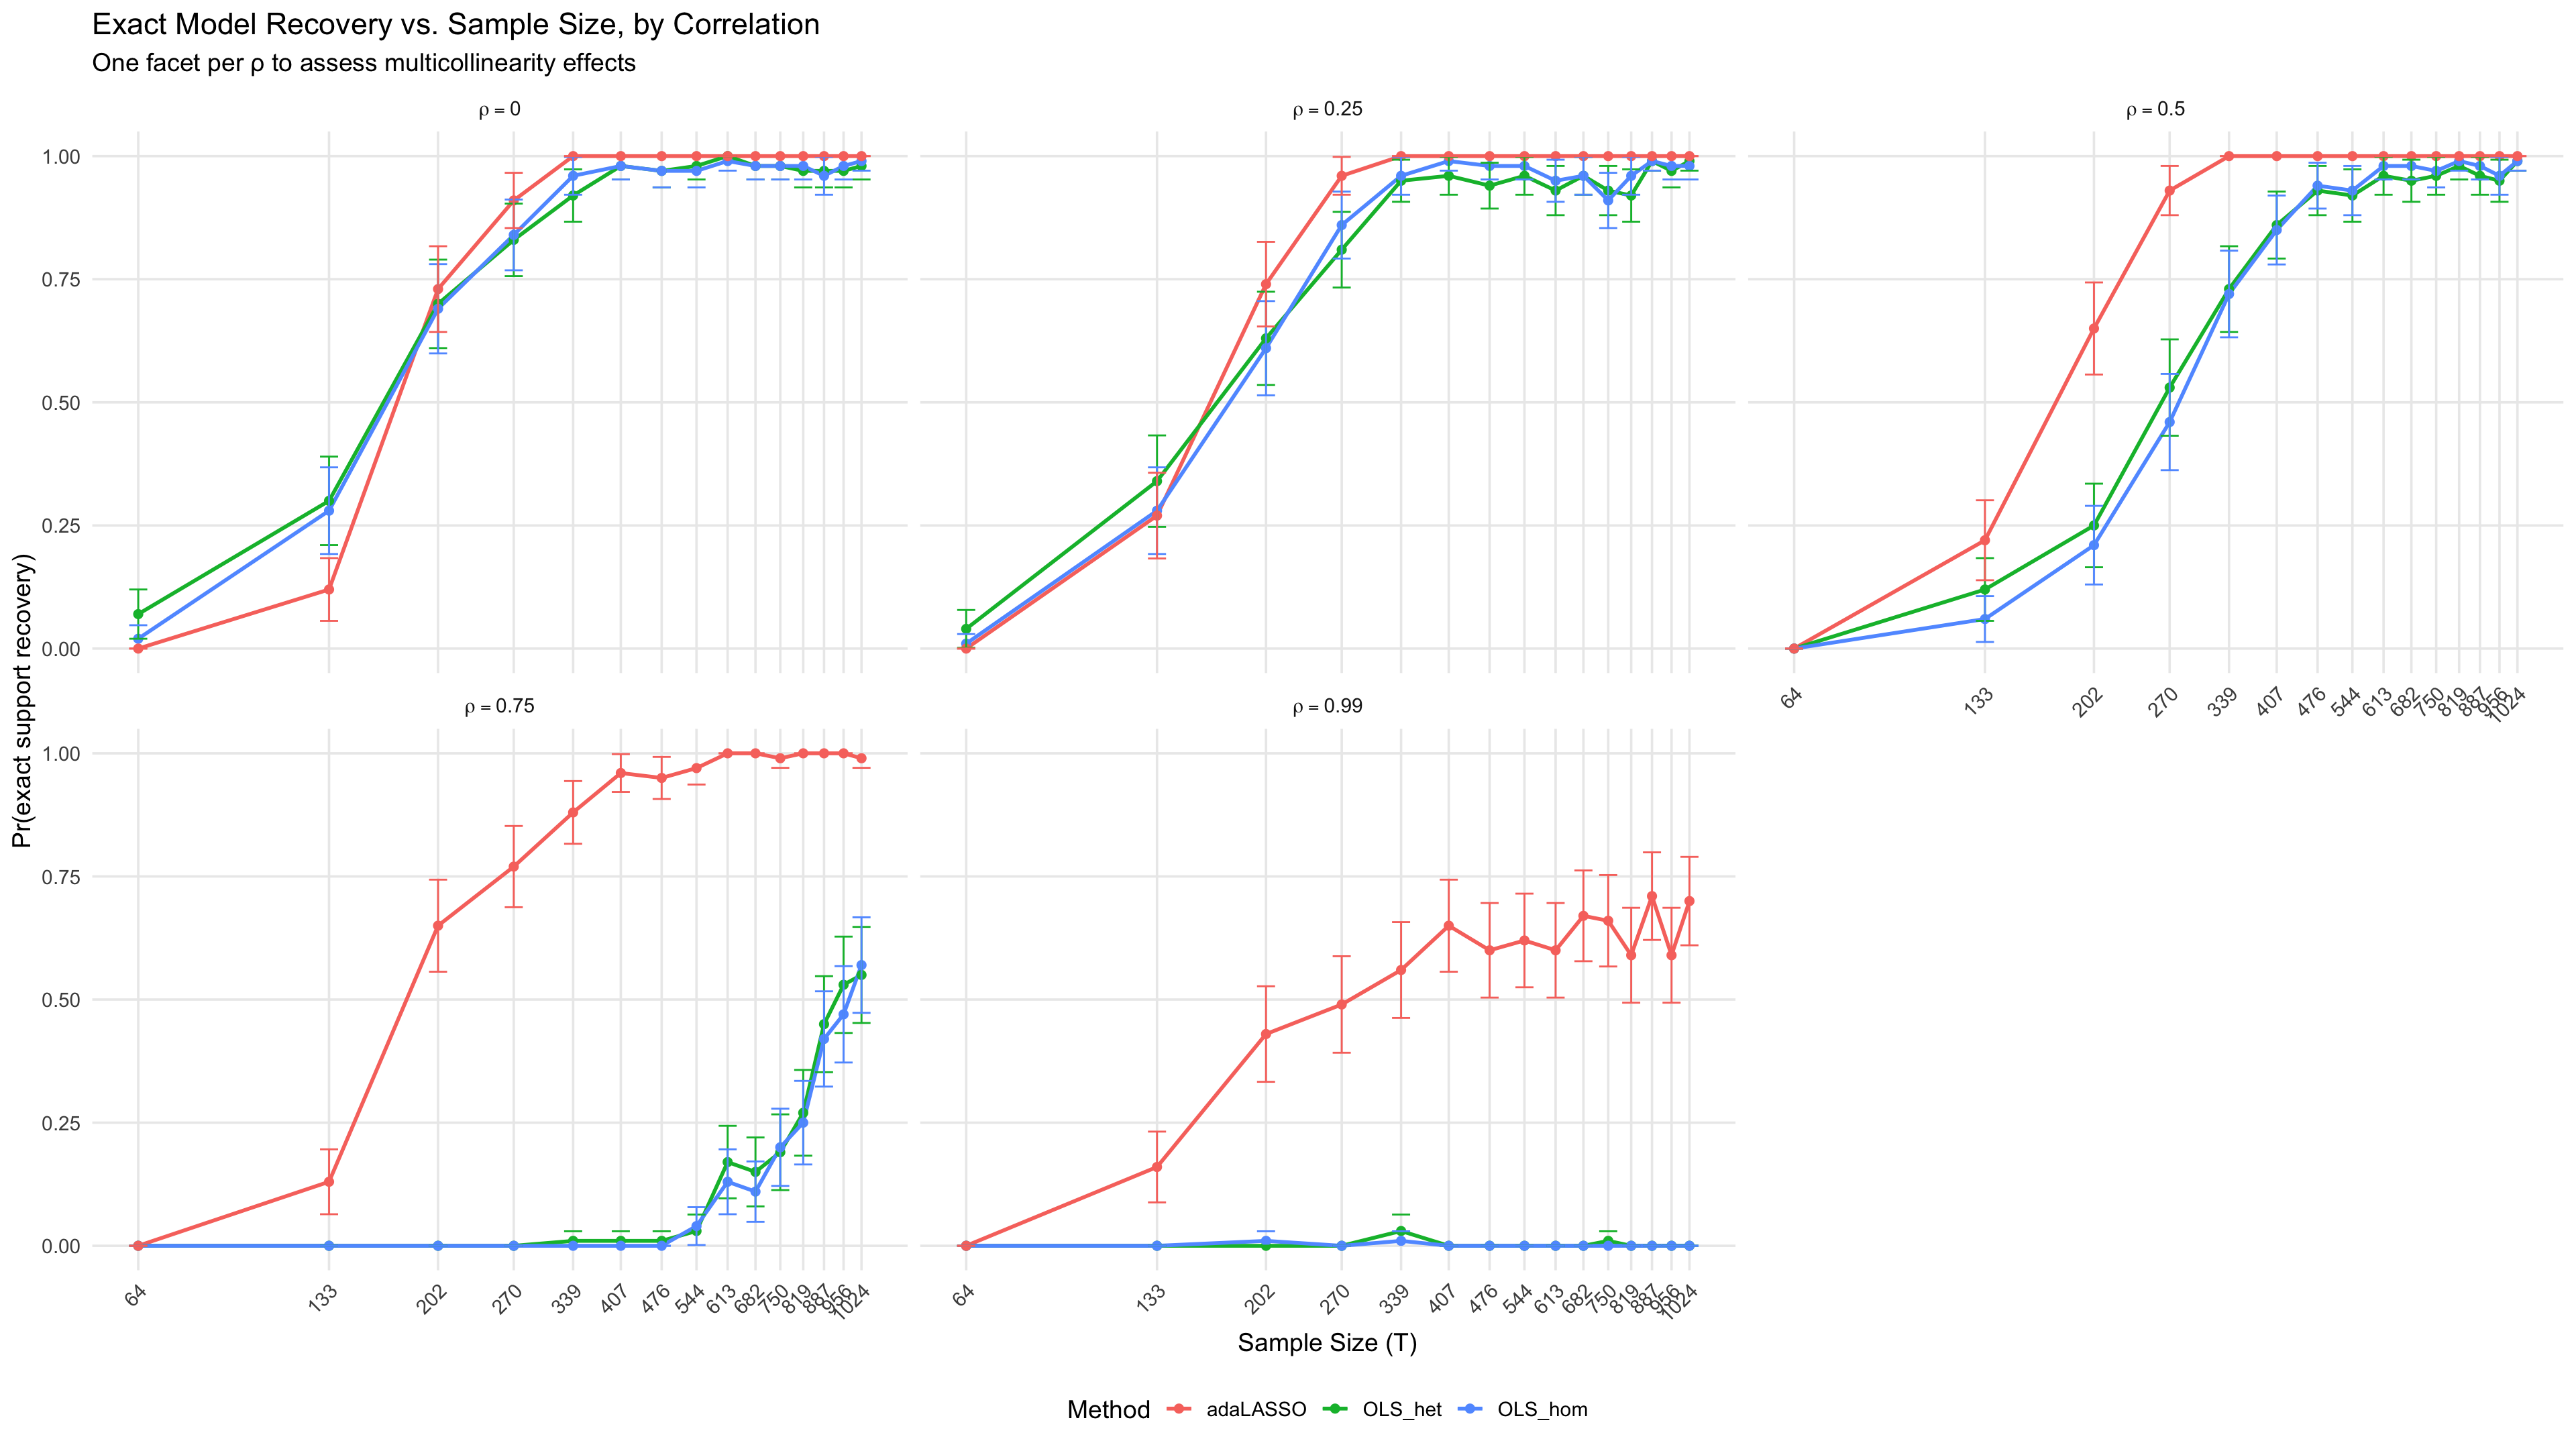
\includegraphics[height=5.5in]{exact_recovery_by_correlation.png}
    \caption{Probability of exact support recovery versus sample size ($T$) for adaptive LASSO (red) and OLS-Bonferroni (blue/green), under varying predictor correlation $\rho$. Each panel corresponds to a different correlation level among predictors (from $\rho=0$ no correlation, up to $\rho=0.99$ extreme collinearity). Error bars (±1.96 SE) are shown for the Monte Carlo estimates.}
    \label{fig:exact_recovery_corr}
\end{sidewaysfigure}

\begin{sidewaysfigure}[h!]
    \centering
    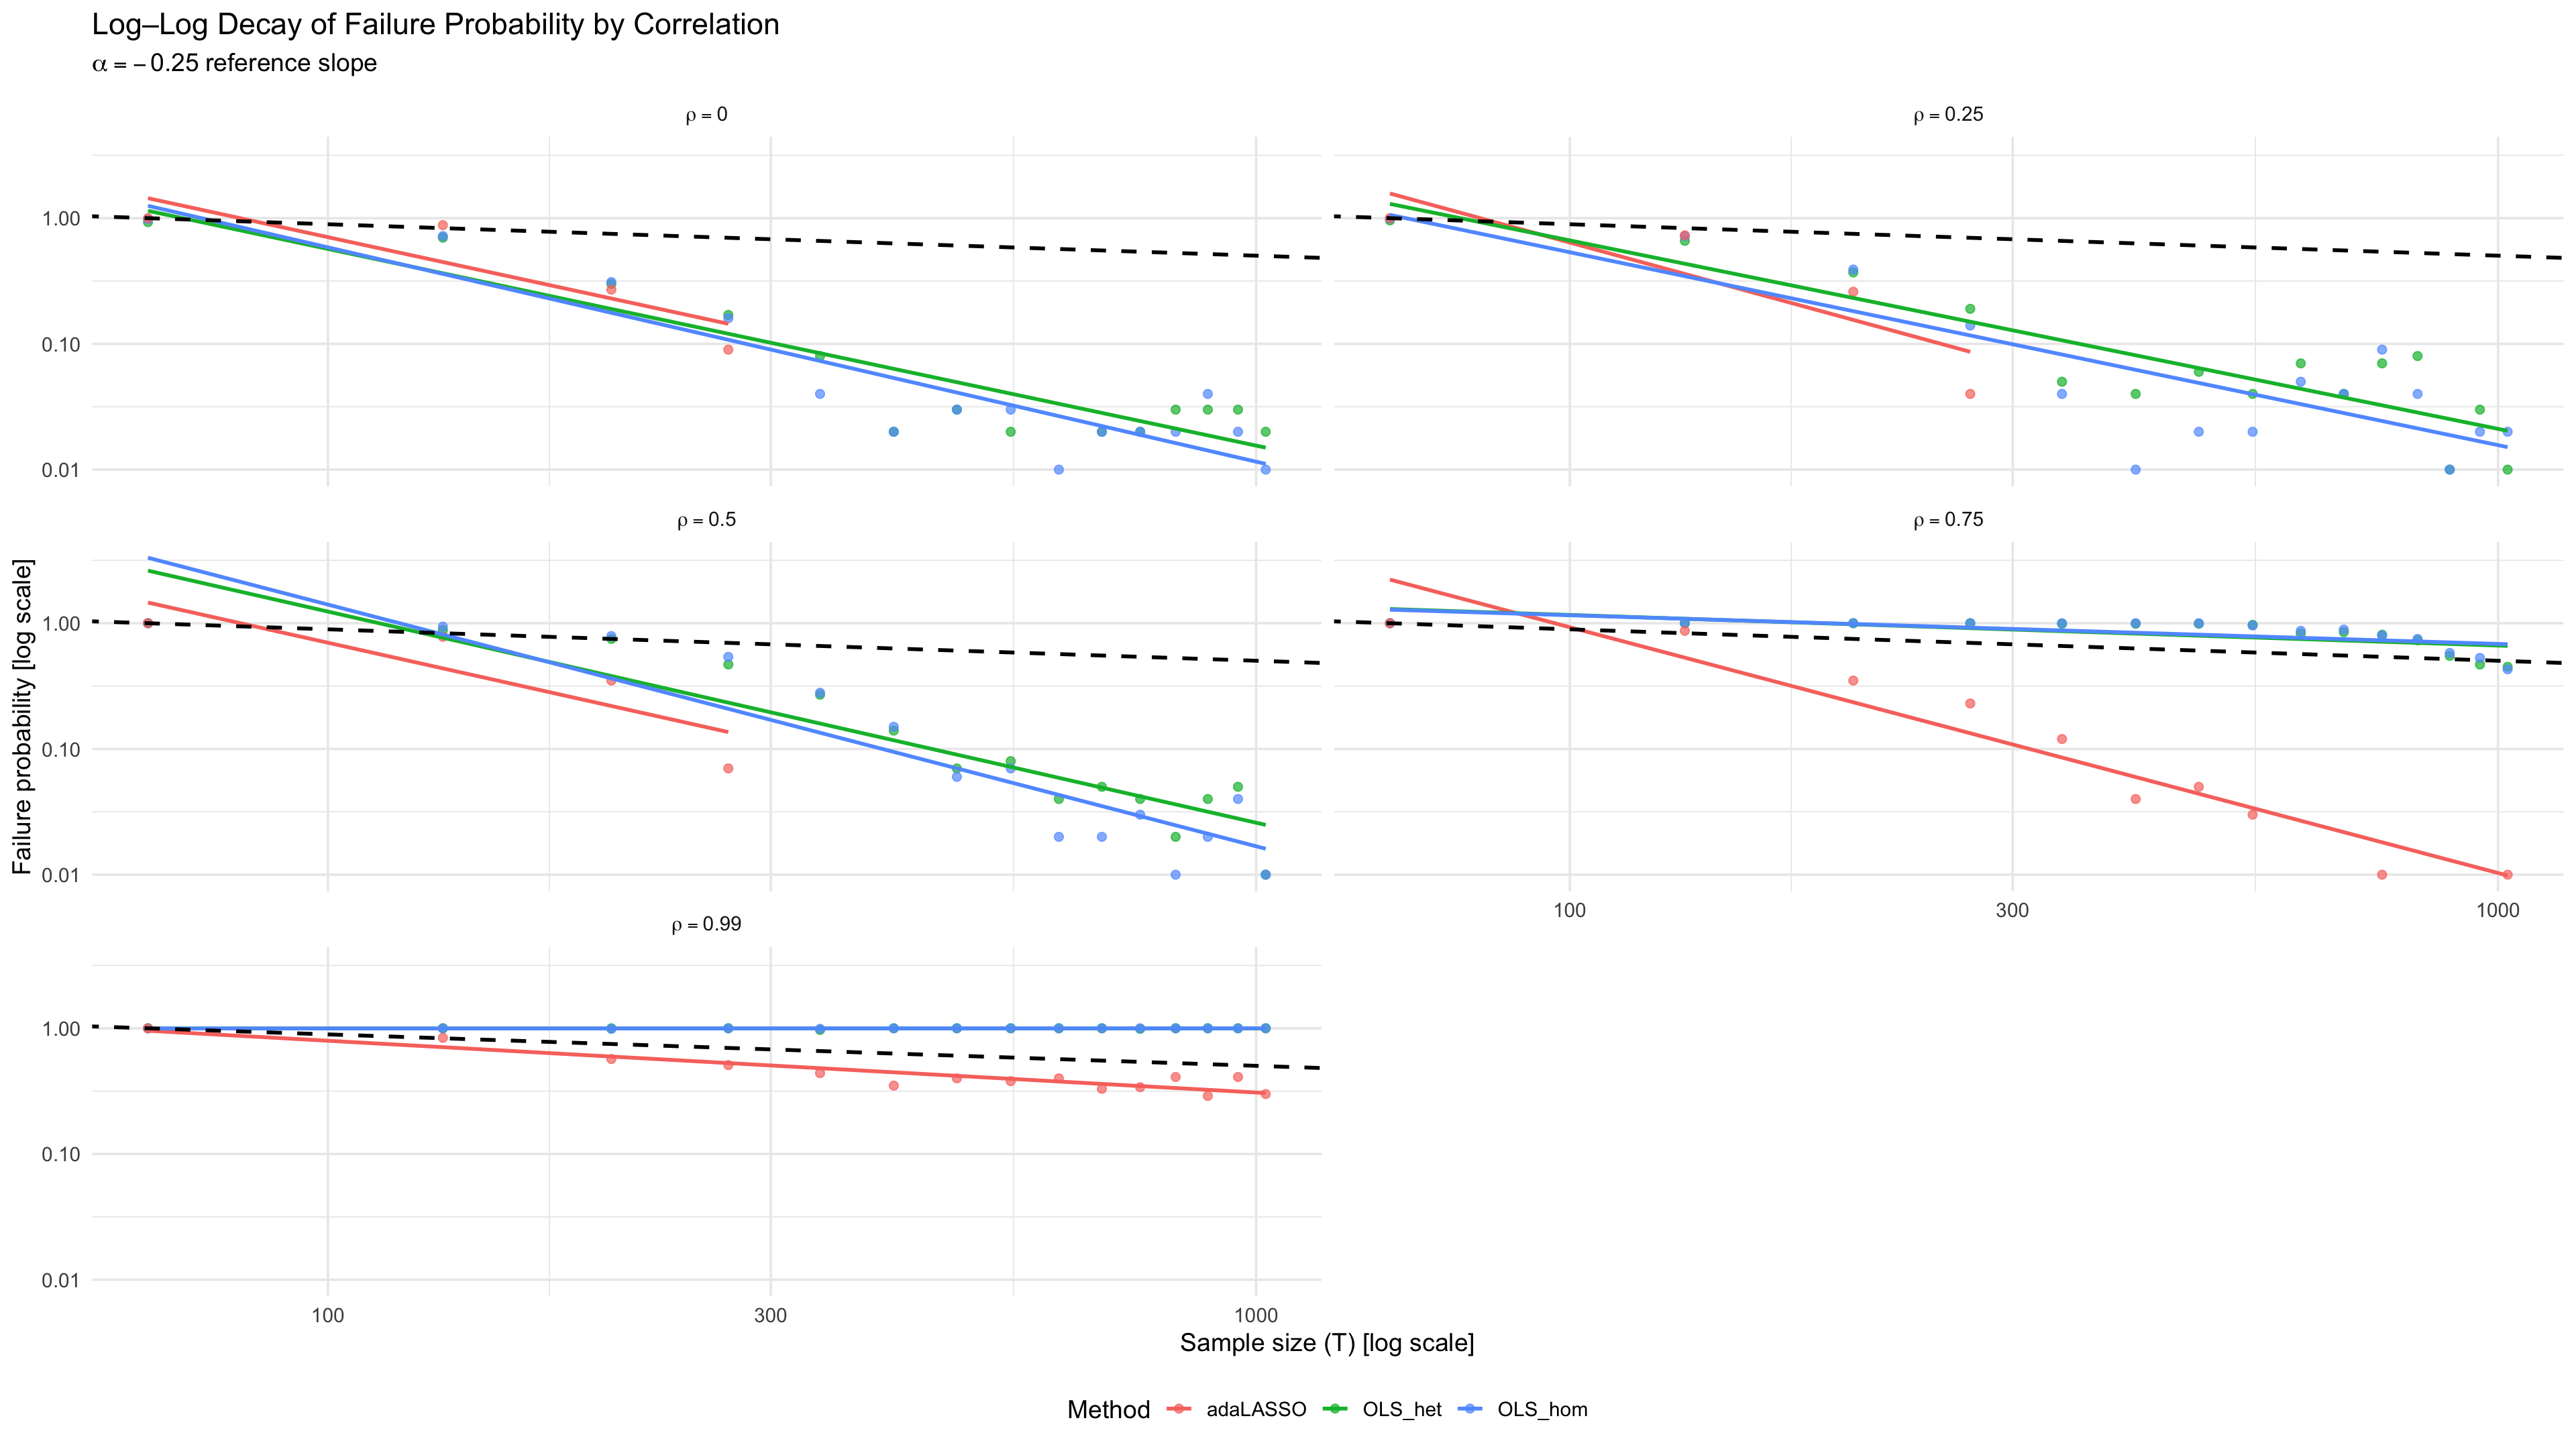
\includegraphics[height=5.5in]{log_log_decay_failure_rate.png}
    \caption{Log–log plot of support recovery failure probability ($\Prob(\mathrm{sign}(\hat{\boldsymbol{\theta}}) \neq \mathrm{sign}(\boldsymbol{\theta}))$) versus sample size $T$, for different correlation levels. Each panel shows the decay of failure probability as $T$ increases on a log–log scale. The red points/line correspond to adaLASSO; blue/green to OLS (homoskedastic or robust OLS, which behave similarly). The black dashed line in each panel indicates a reference slope of $-0.25$ (a power-law $T^{-0.25}$) as a guide.}
    \label{fig:log_log_failure_rate_corr}
\end{sidewaysfigure}

\begin{sidewaysfigure}[h!]
    \centering
    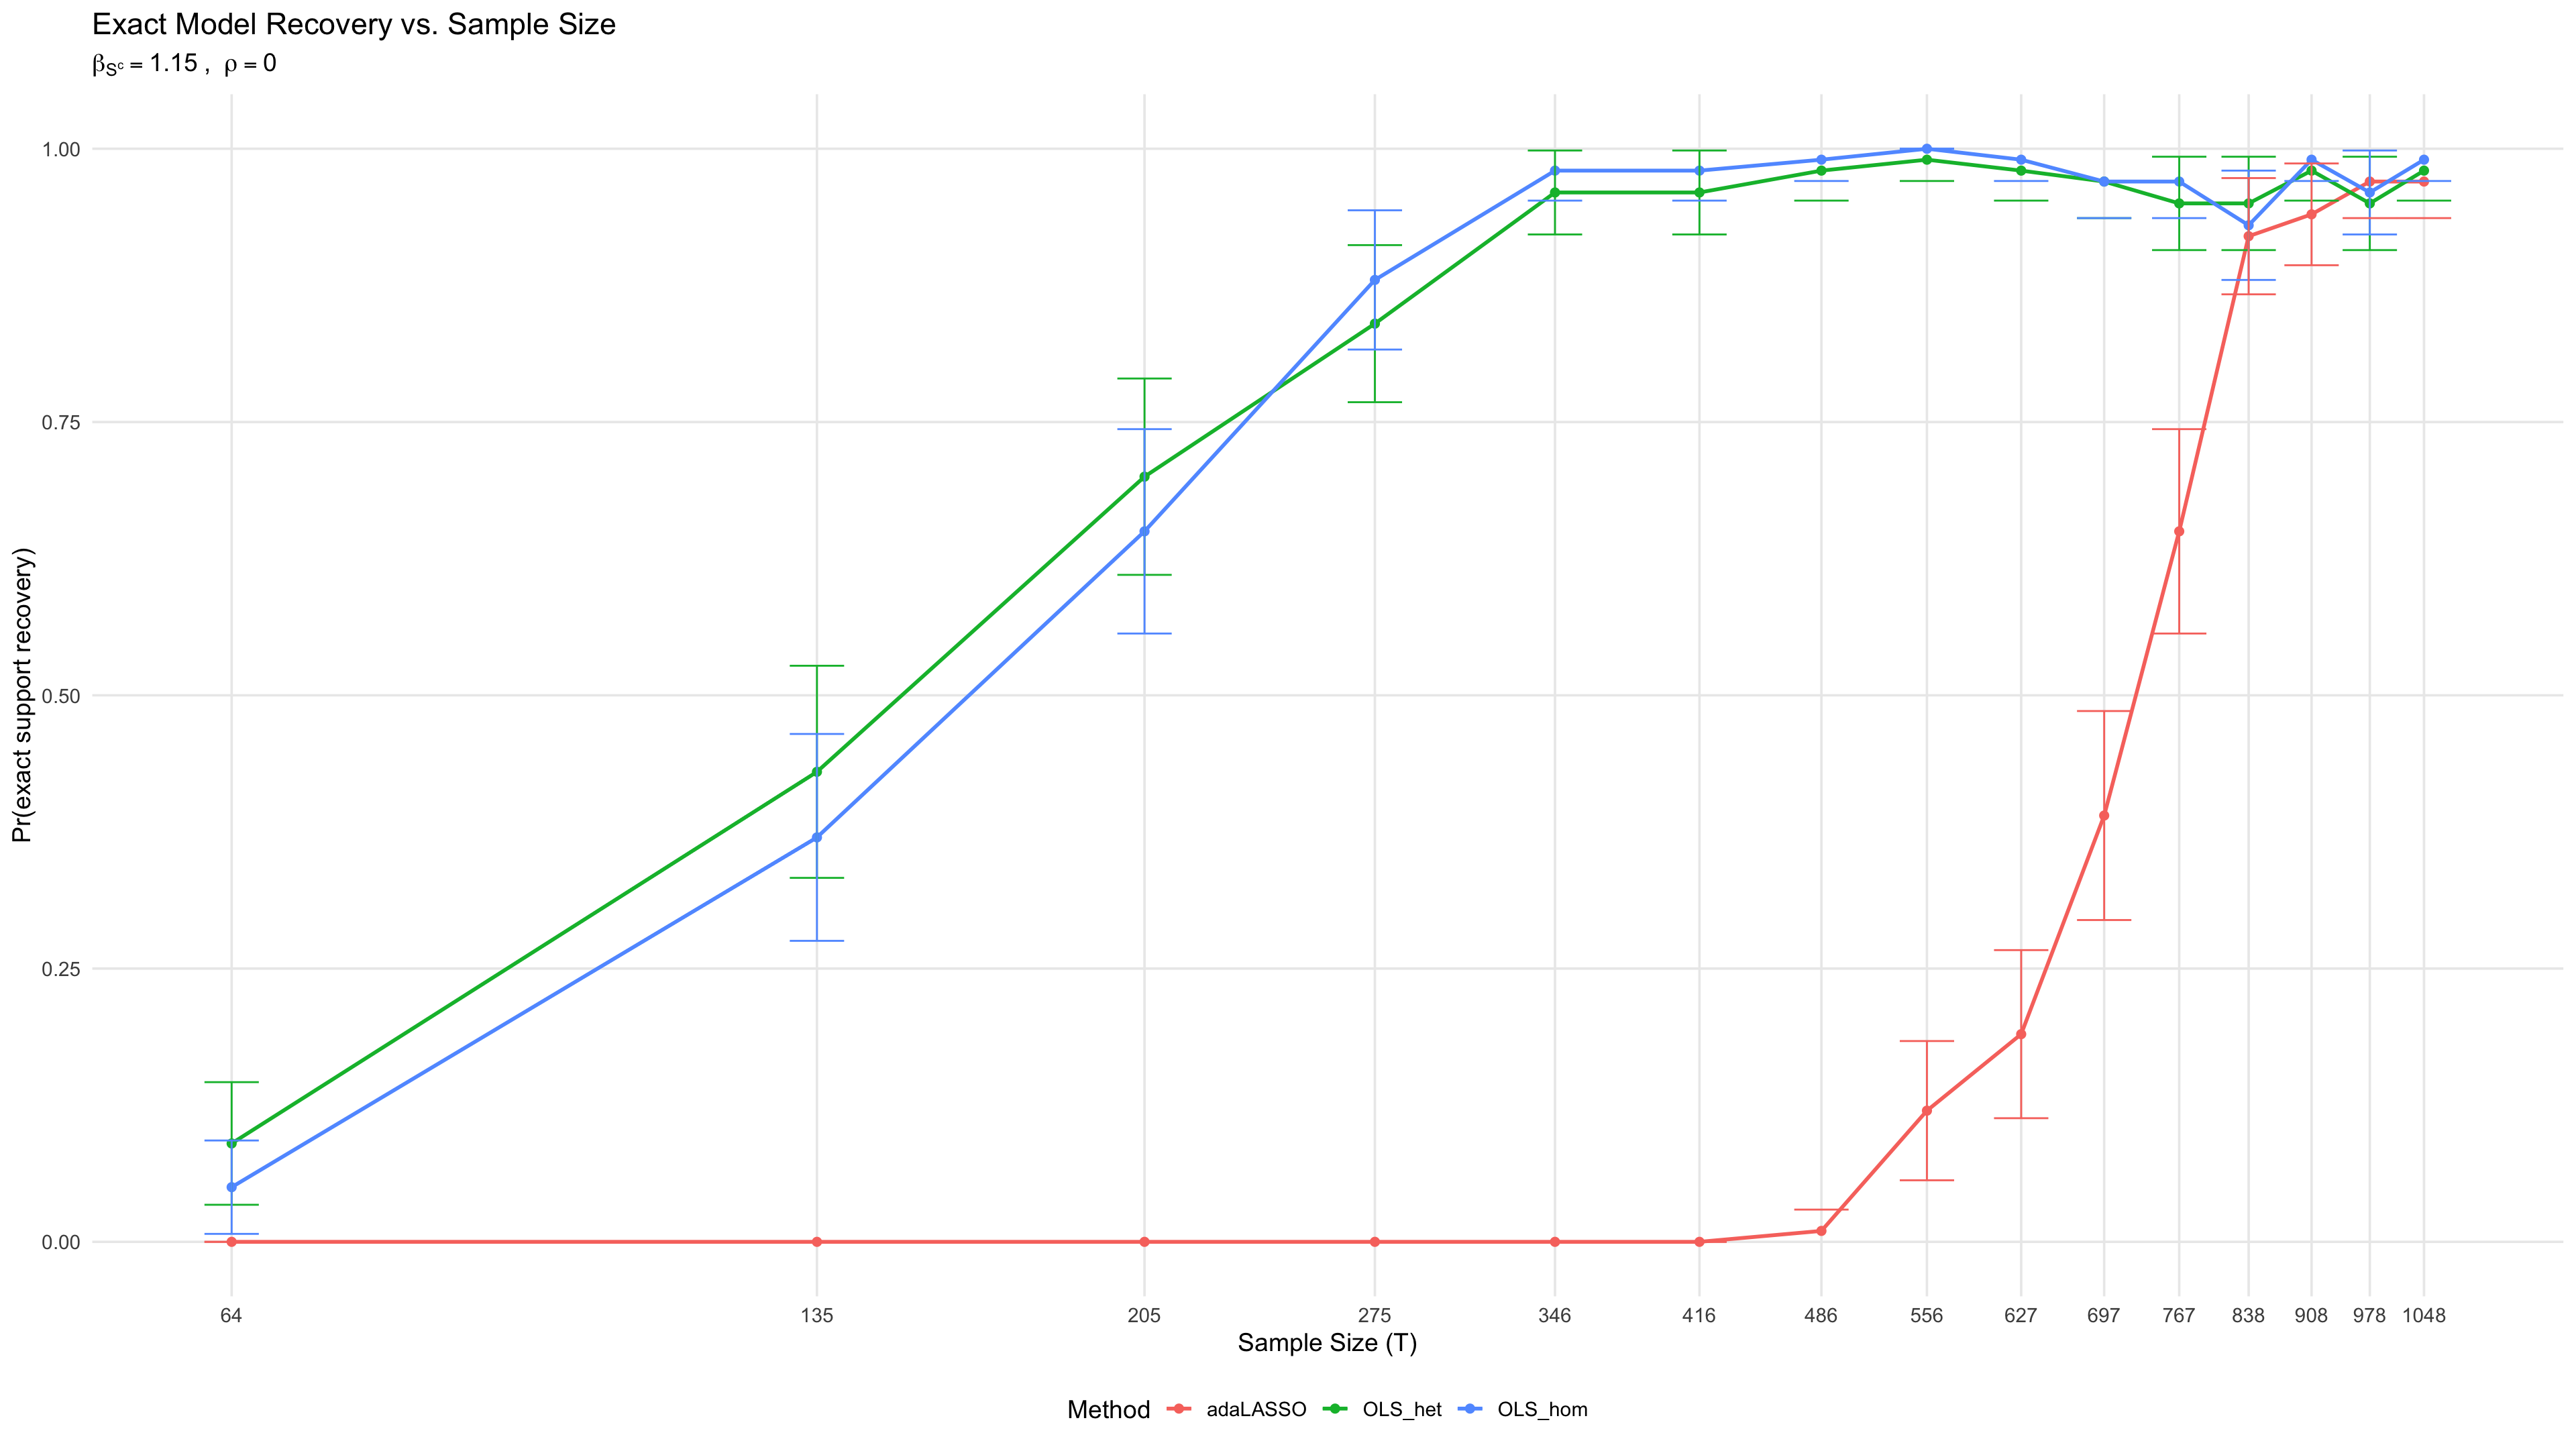
\includegraphics[height=5in]{exact_recovery_low_beta_Sc.png}
    \caption{Probability of exact support recovery versus sample size ($T$) for adaptive LASSO (red) and OLS-Bonferroni (blue/green), under uncorrelated covariates and a comparatively slower discrimination rate $\beta_{S^c} = 1.15$.}
    \label{fig:exact_recovery_beta}
\end{sidewaysfigure}

\begin{sidewaysfigure}[h!]
    \centering
    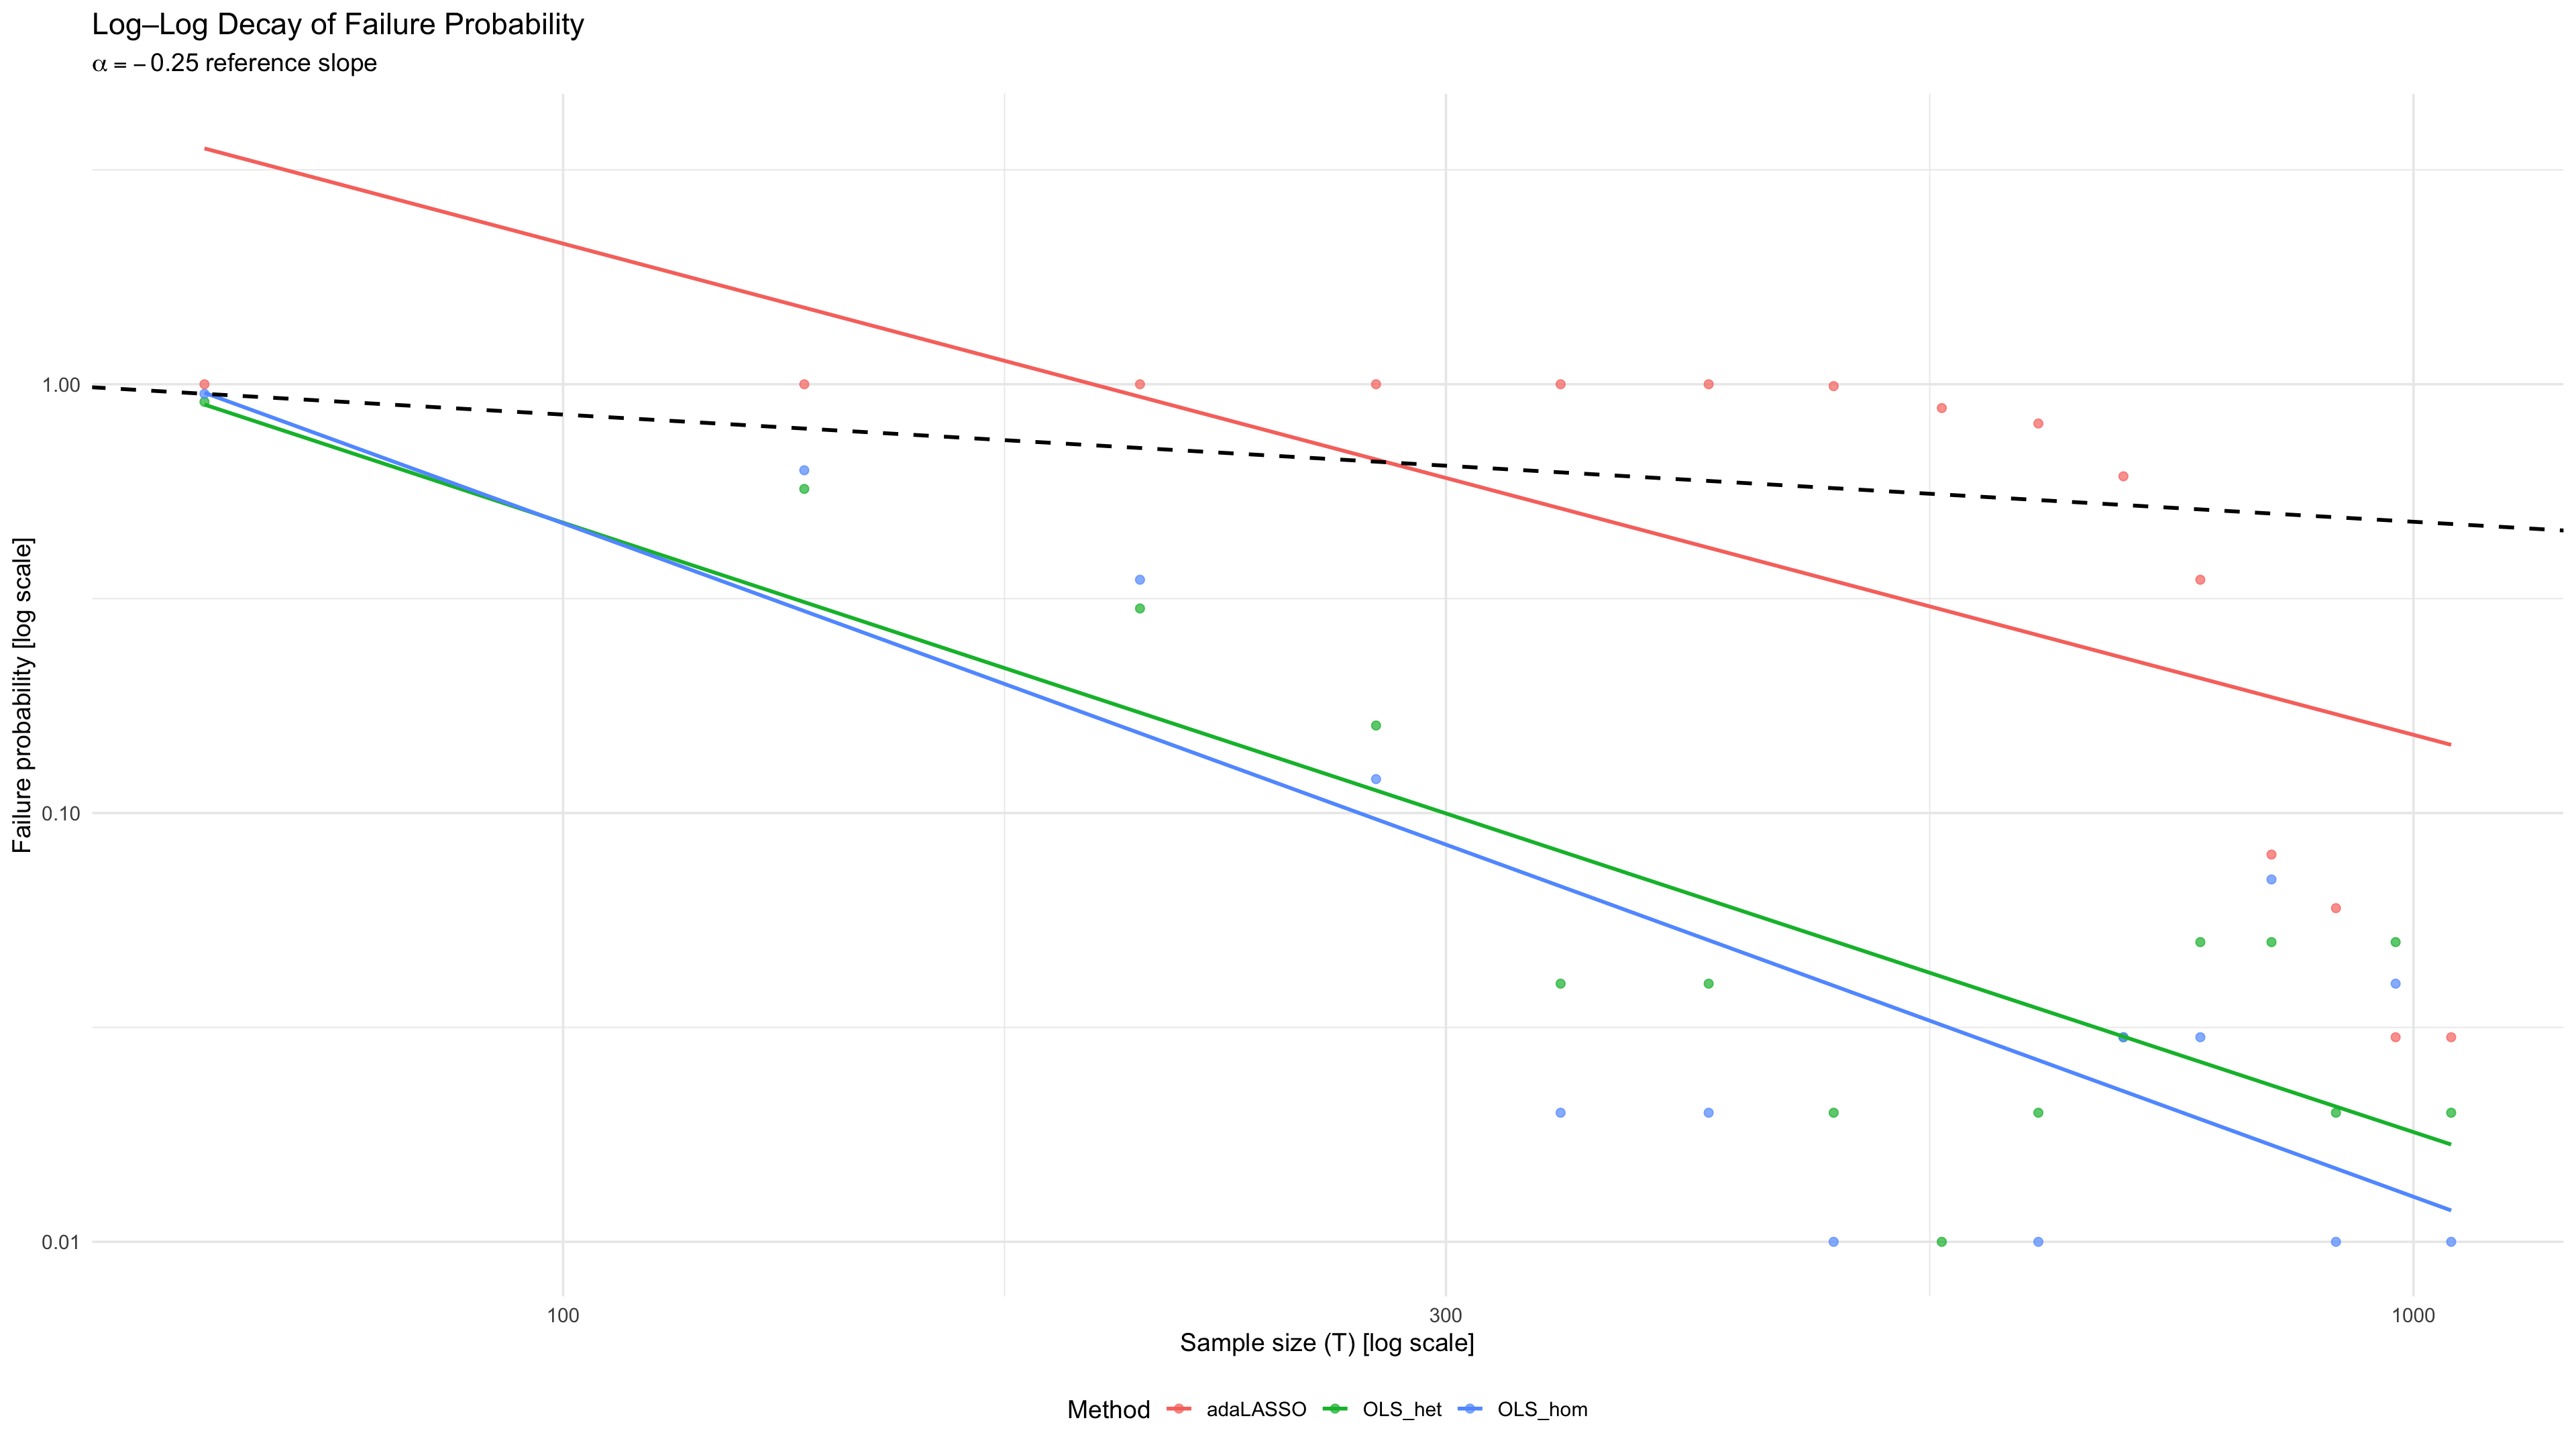
\includegraphics[height=5in]{log_log_decay_low_beta_sc.png}
    \caption{Log–log plot of support recovery failure probability ($\Prob(\mathrm{sign}(\hat{\boldsymbol{\theta}}) \neq \mathrm{sign}(\boldsymbol{\theta}))$) versus sample size $T$, assuming uncorrelated variables and a comparatively slower discrimination rate $\beta_{S^c} = 1.15$.}
    \label{fig:log_log_failure_rate_beta}
\end{sidewaysfigure}

% Please add the following packages to your preamble:
% \usepackage{booktabs}
% \usepackage{multirow}
% \usepackage{longtable}

\begin{longtable}{@{}lll@{}}
\caption{Base configuration used in synthetic data experiments.} 
\label{tab:base_config} \\
\toprule
\textbf{Category} & \textbf{Parameter} & \textbf{Value} \\ \midrule
\endfirsthead

\multicolumn{3}{c}%
{{\bfseries Table \thetable\ (continued)}} \\
\toprule
\textbf{Category} & \textbf{Parameter} & \textbf{Value} \\ \midrule
\endhead

\bottomrule
\endfoot

\multirow{8}{*}{General} 
 & Ticker & SIM (Simulated LOB) \\
 & $\Delta^B$ & $5{'}000{,}000.0$ uot \\
 & $\Delta^A$ & $100{,}000.0$ uot \\
 & $\delta$ & $100.0$ uot \\
 & Seed & 19991810 \\
 & Session start & 0.0 uot \\
 & Session finish & $10{'}000{,}000.0$ uot \\
 & Target Variable & $r^w$ \\ \midrule

\multirow{10}{*}{Backbone} 
 & Training Epochs & 10 \\
 & Batch size & 32 \\
 & Validation proportion & 0.1 \\
 & Buffer proportion & 0.05 \\
 & Windsorization quantile & 0.005 \\
 & ADF rejection threshold & 0.8 \\
 & KPSS verification threshold & 0.2 \\
 & NA threshold & 0.1 \\
 & Learning rate & 0.0001 \\
 & Correlation threshold & 0.95 \\ \midrule

\multirow{9}{*}{Interface} 
 & $\alpha$  & \{0.0, 0.1, 0.25, 0.5, 0.75, 0.9, 1.0\} \\
 & $\lambda_1$ & $\mathrm{logspace}(-4,1,25)$ \\
 & $\tau$   & \{0.25, 0.5, 1.0, 1.5, 2.0\} \\
 & $\lambda_2$ & $\mathrm{logspace}(0,1,25)$ \\
 & Validation proportion & 0.2 \\
 & Selection threshold & 0.17 ($L = 50$, $\alpha = 0.00005$) \\
 & Tolerance threshold & $10^{-6}$ \\
 & OLS significance level & 0.05 \\
 & Surrogate model lags & 5 \\ \midrule

\multirow{3}{*}{Adapter} 
 & ARMA order & (1,1) \\
 & GARCH order & (1,1) \\
 & Error distribution & Skewed t \\
\end{longtable} 

\begin{figure}[ht!]
\centering

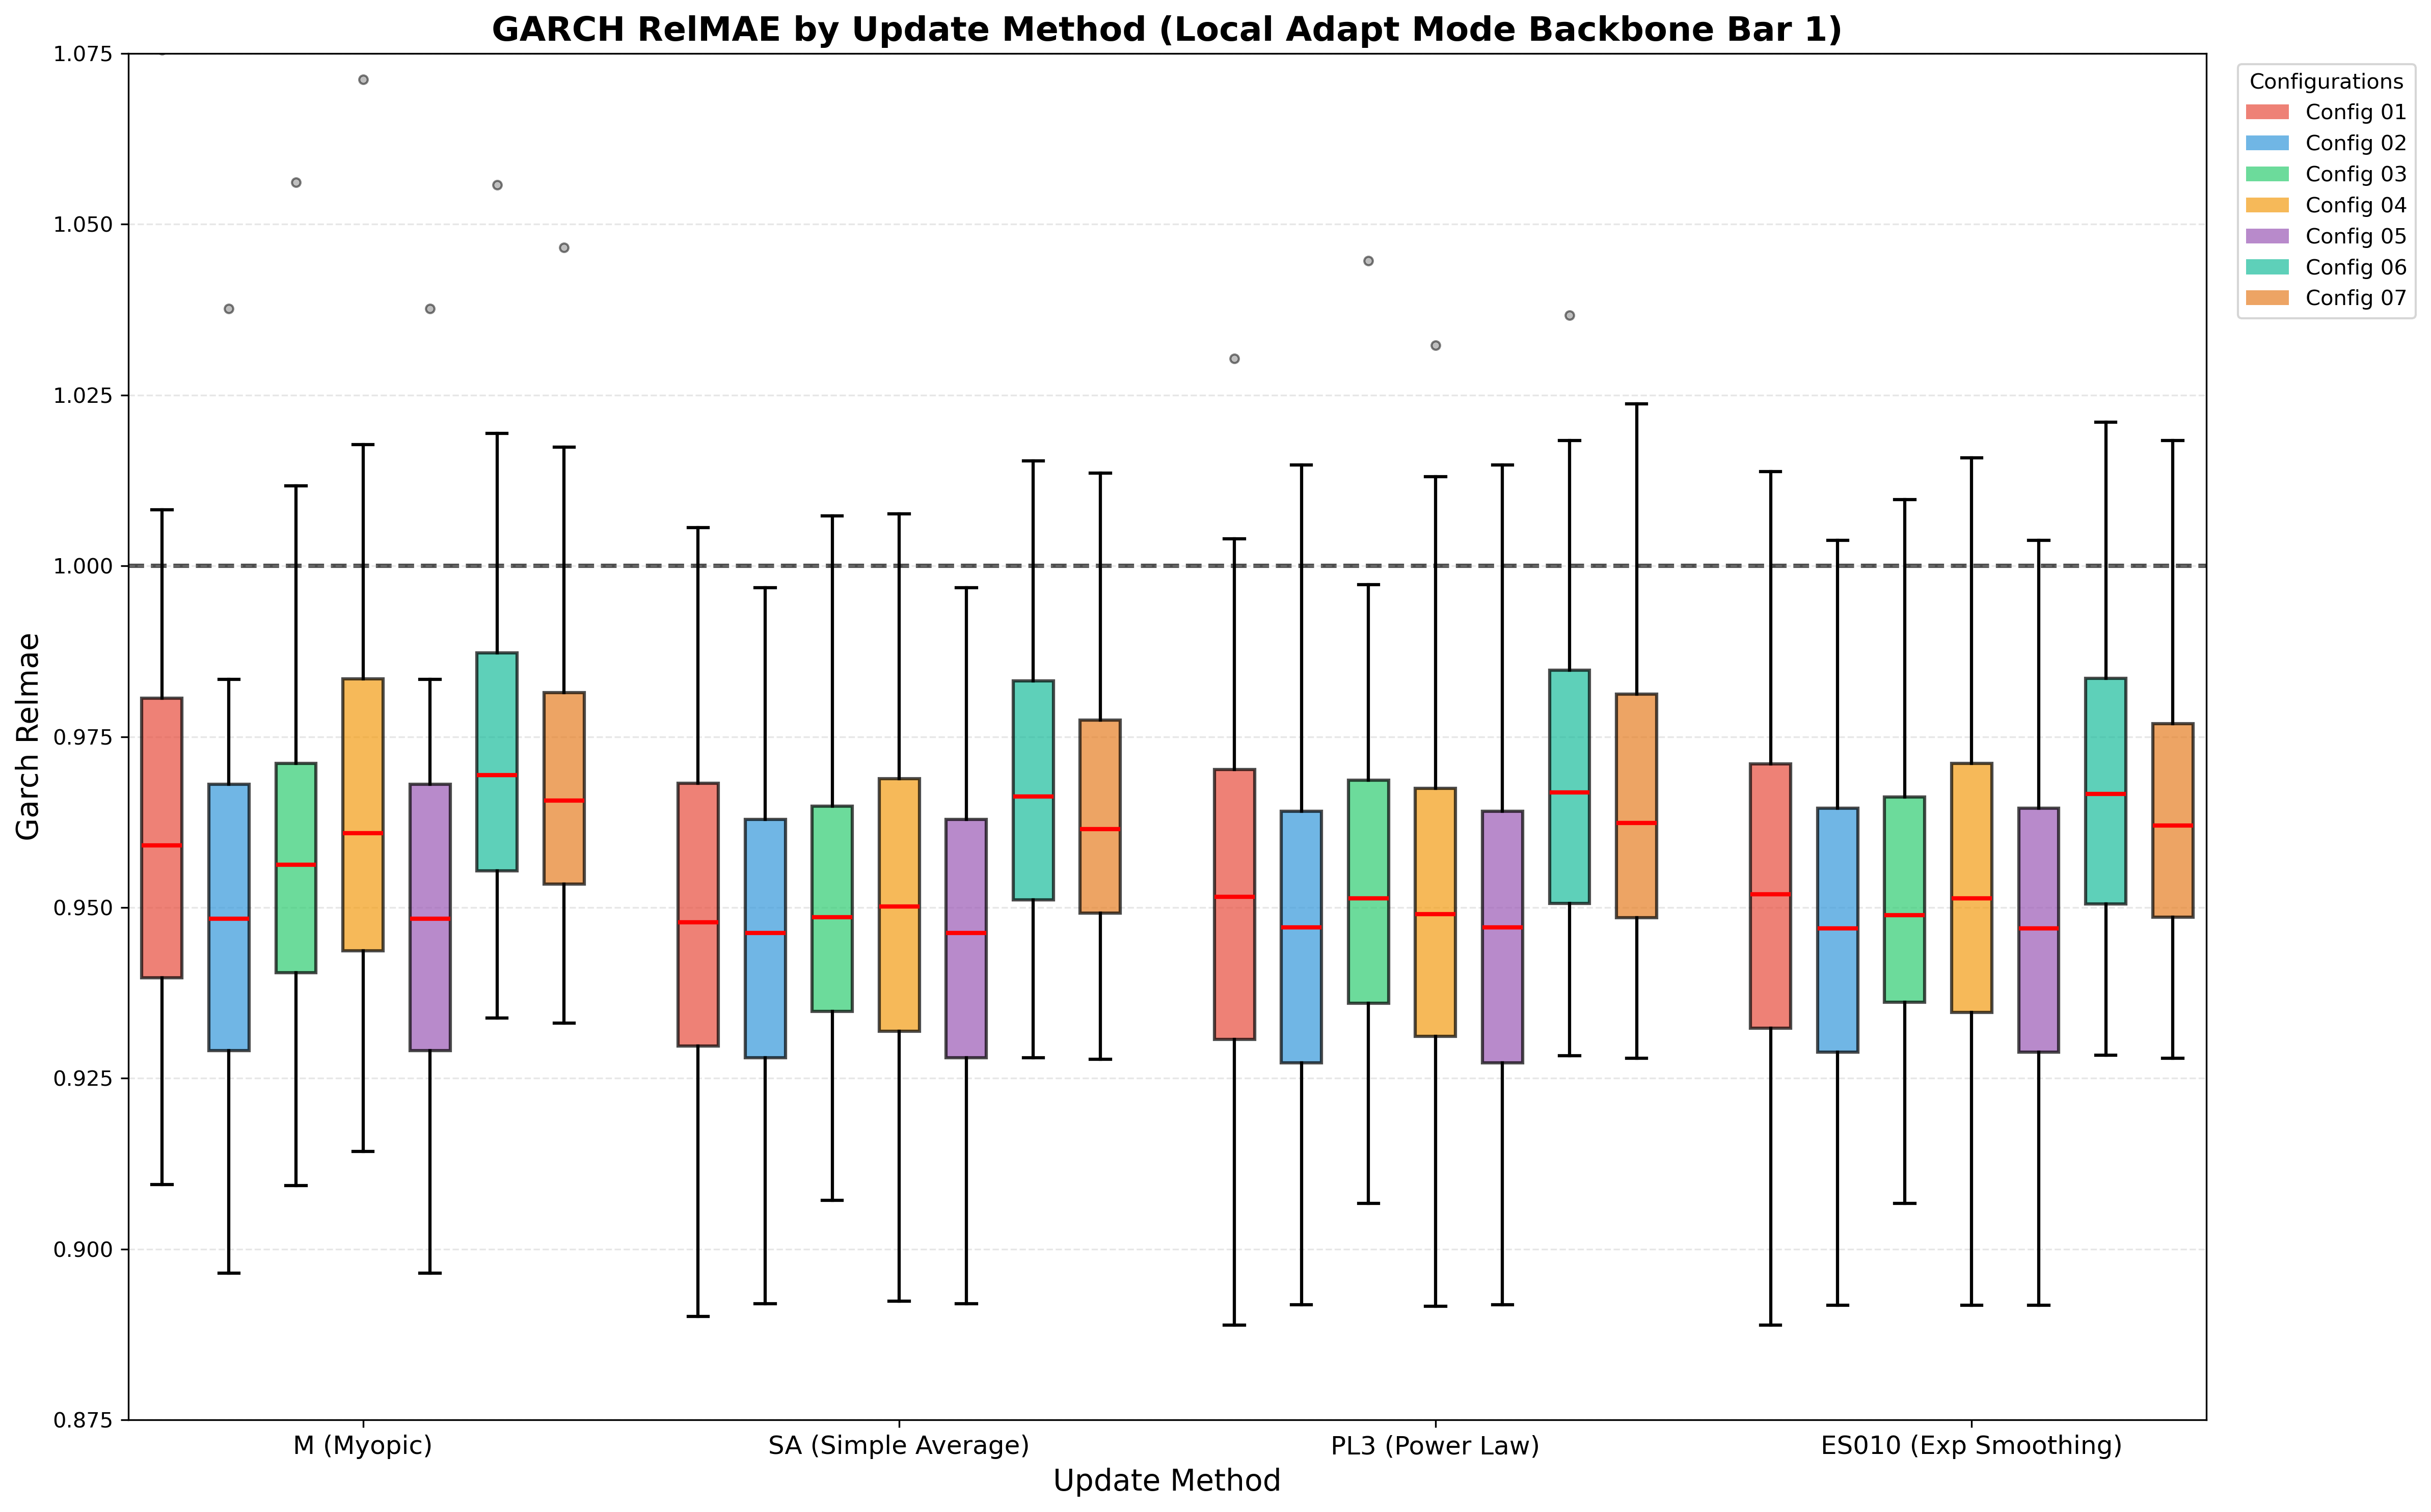
\includegraphics[width=0.85\linewidth]{performance_boxplot_bb000.png}
\vspace{0.5em}
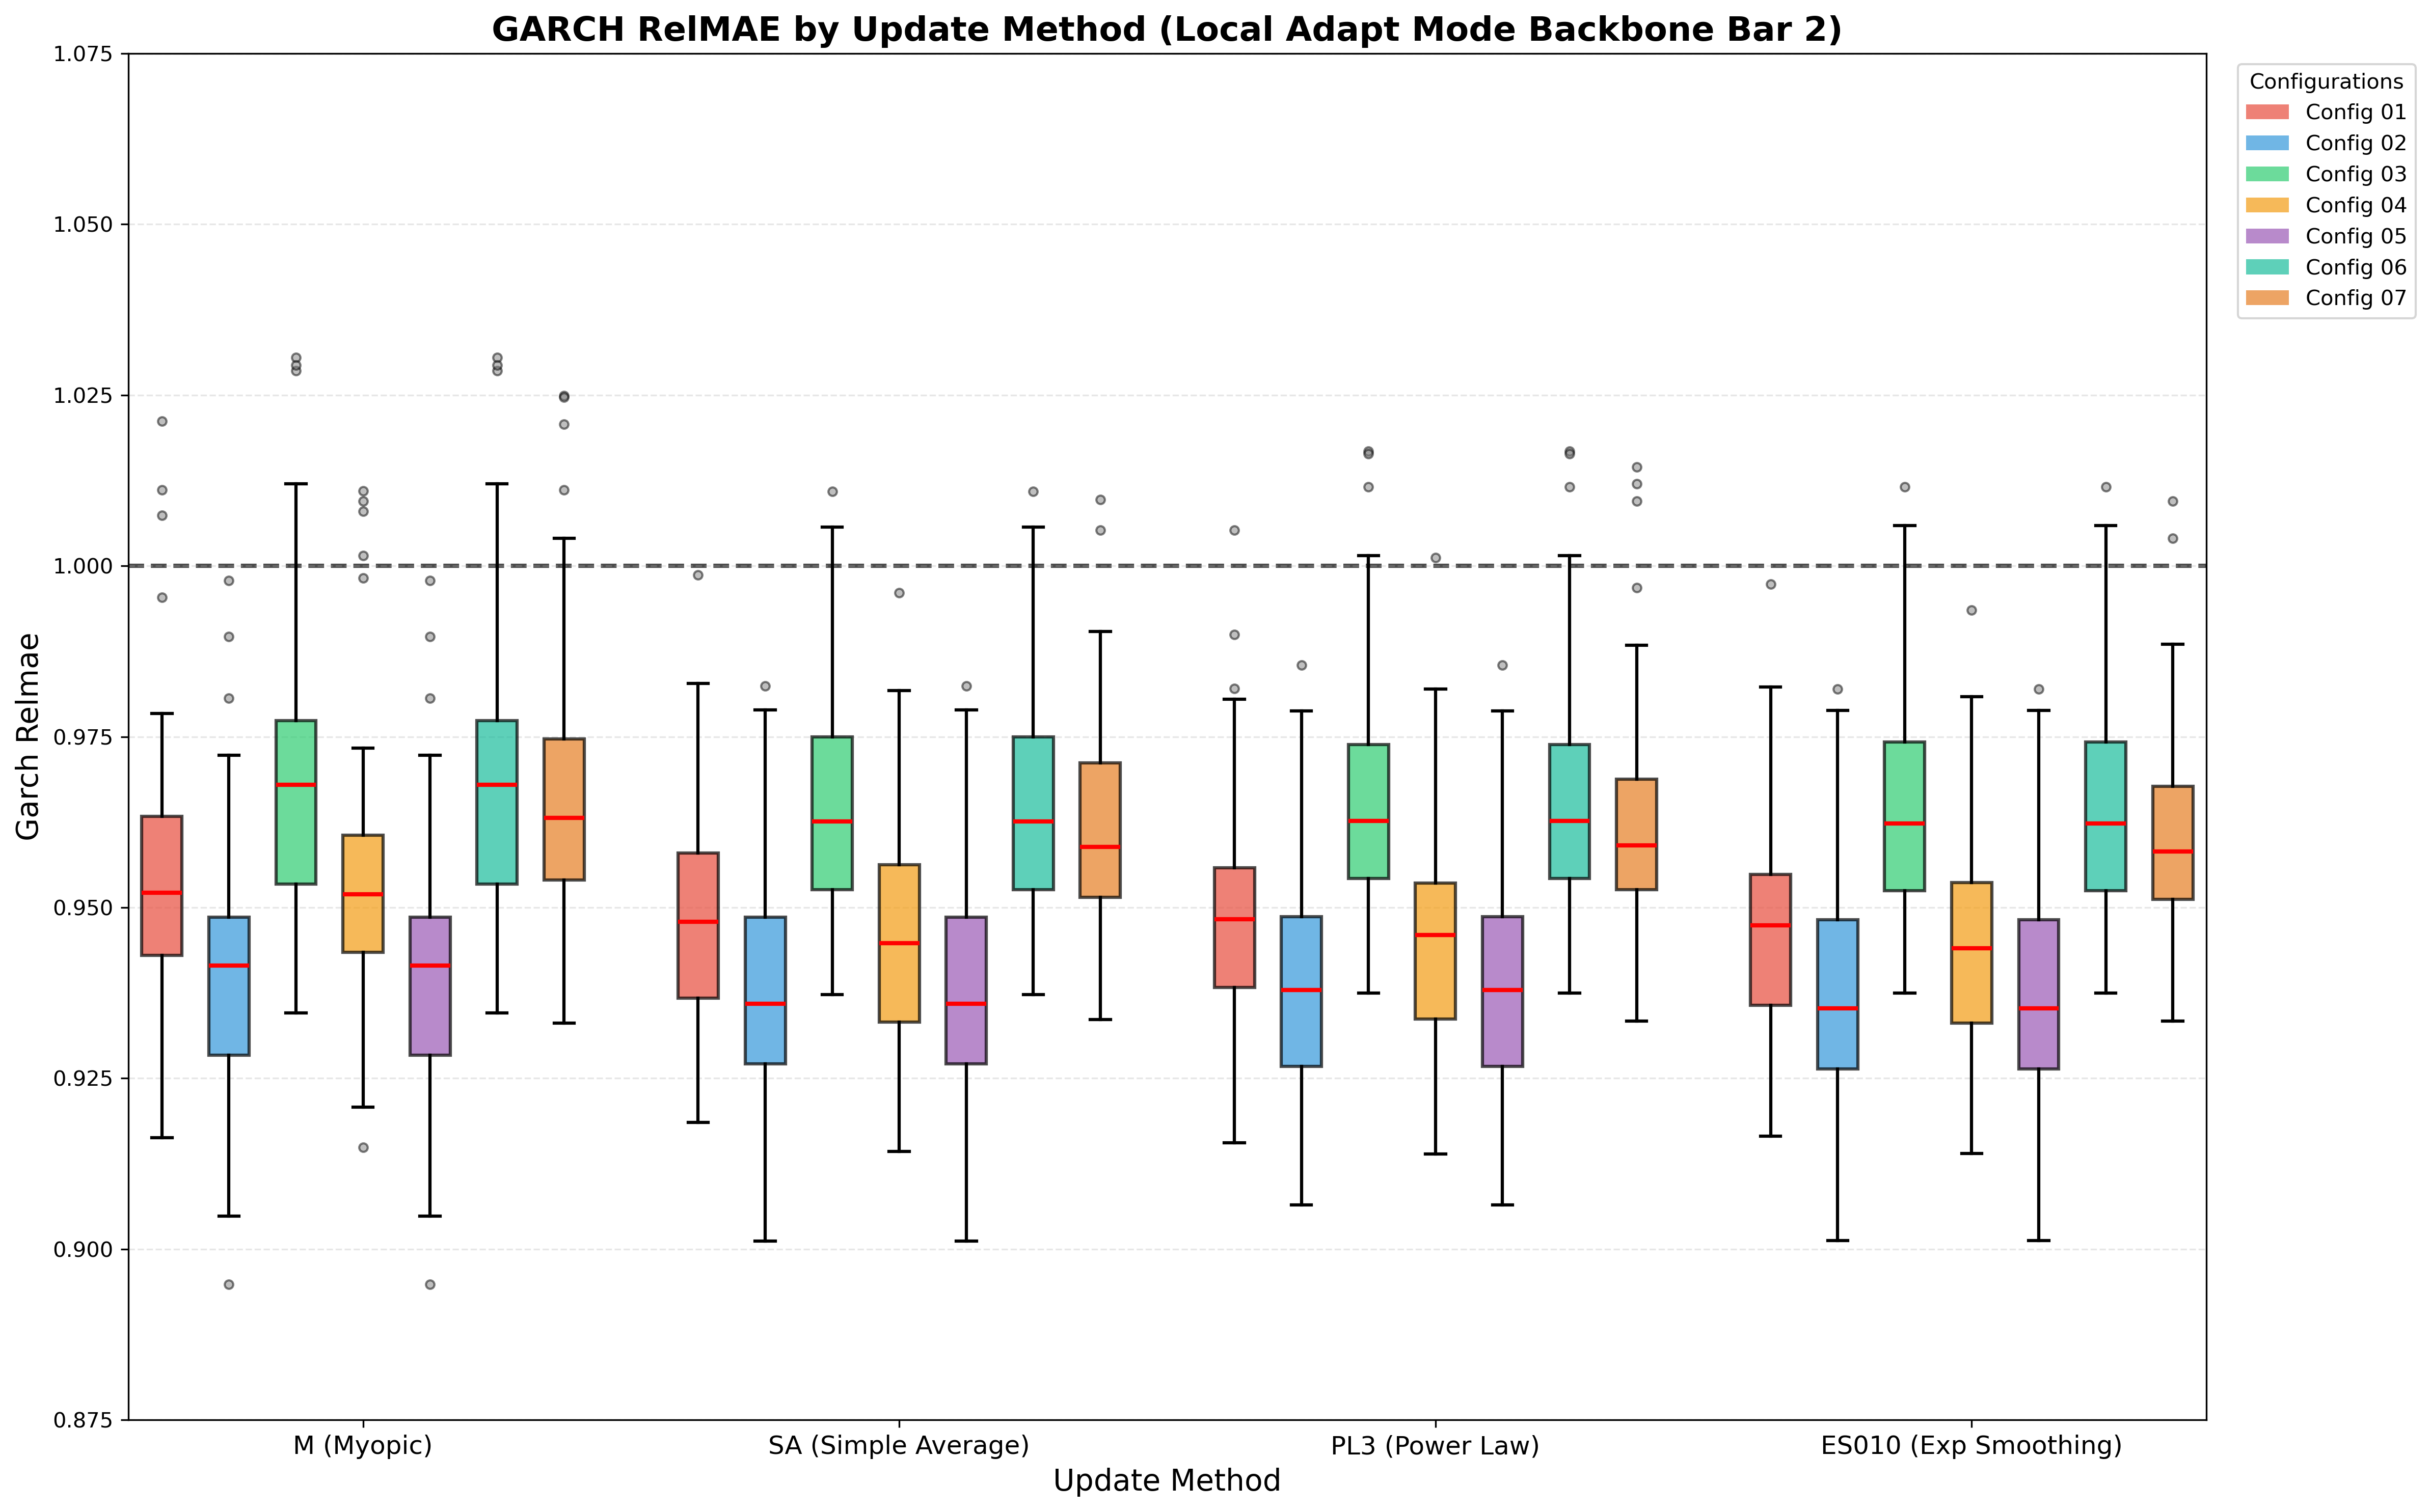
\includegraphics[width=0.85\linewidth]{performance_boxplot_bb001.png}

\caption{GARCH RelMAE comparison across update methods and configurations.}
\label{fig:garch_relmae_vertical}
\end{figure}

\begin{figure}[ht!]
\centering

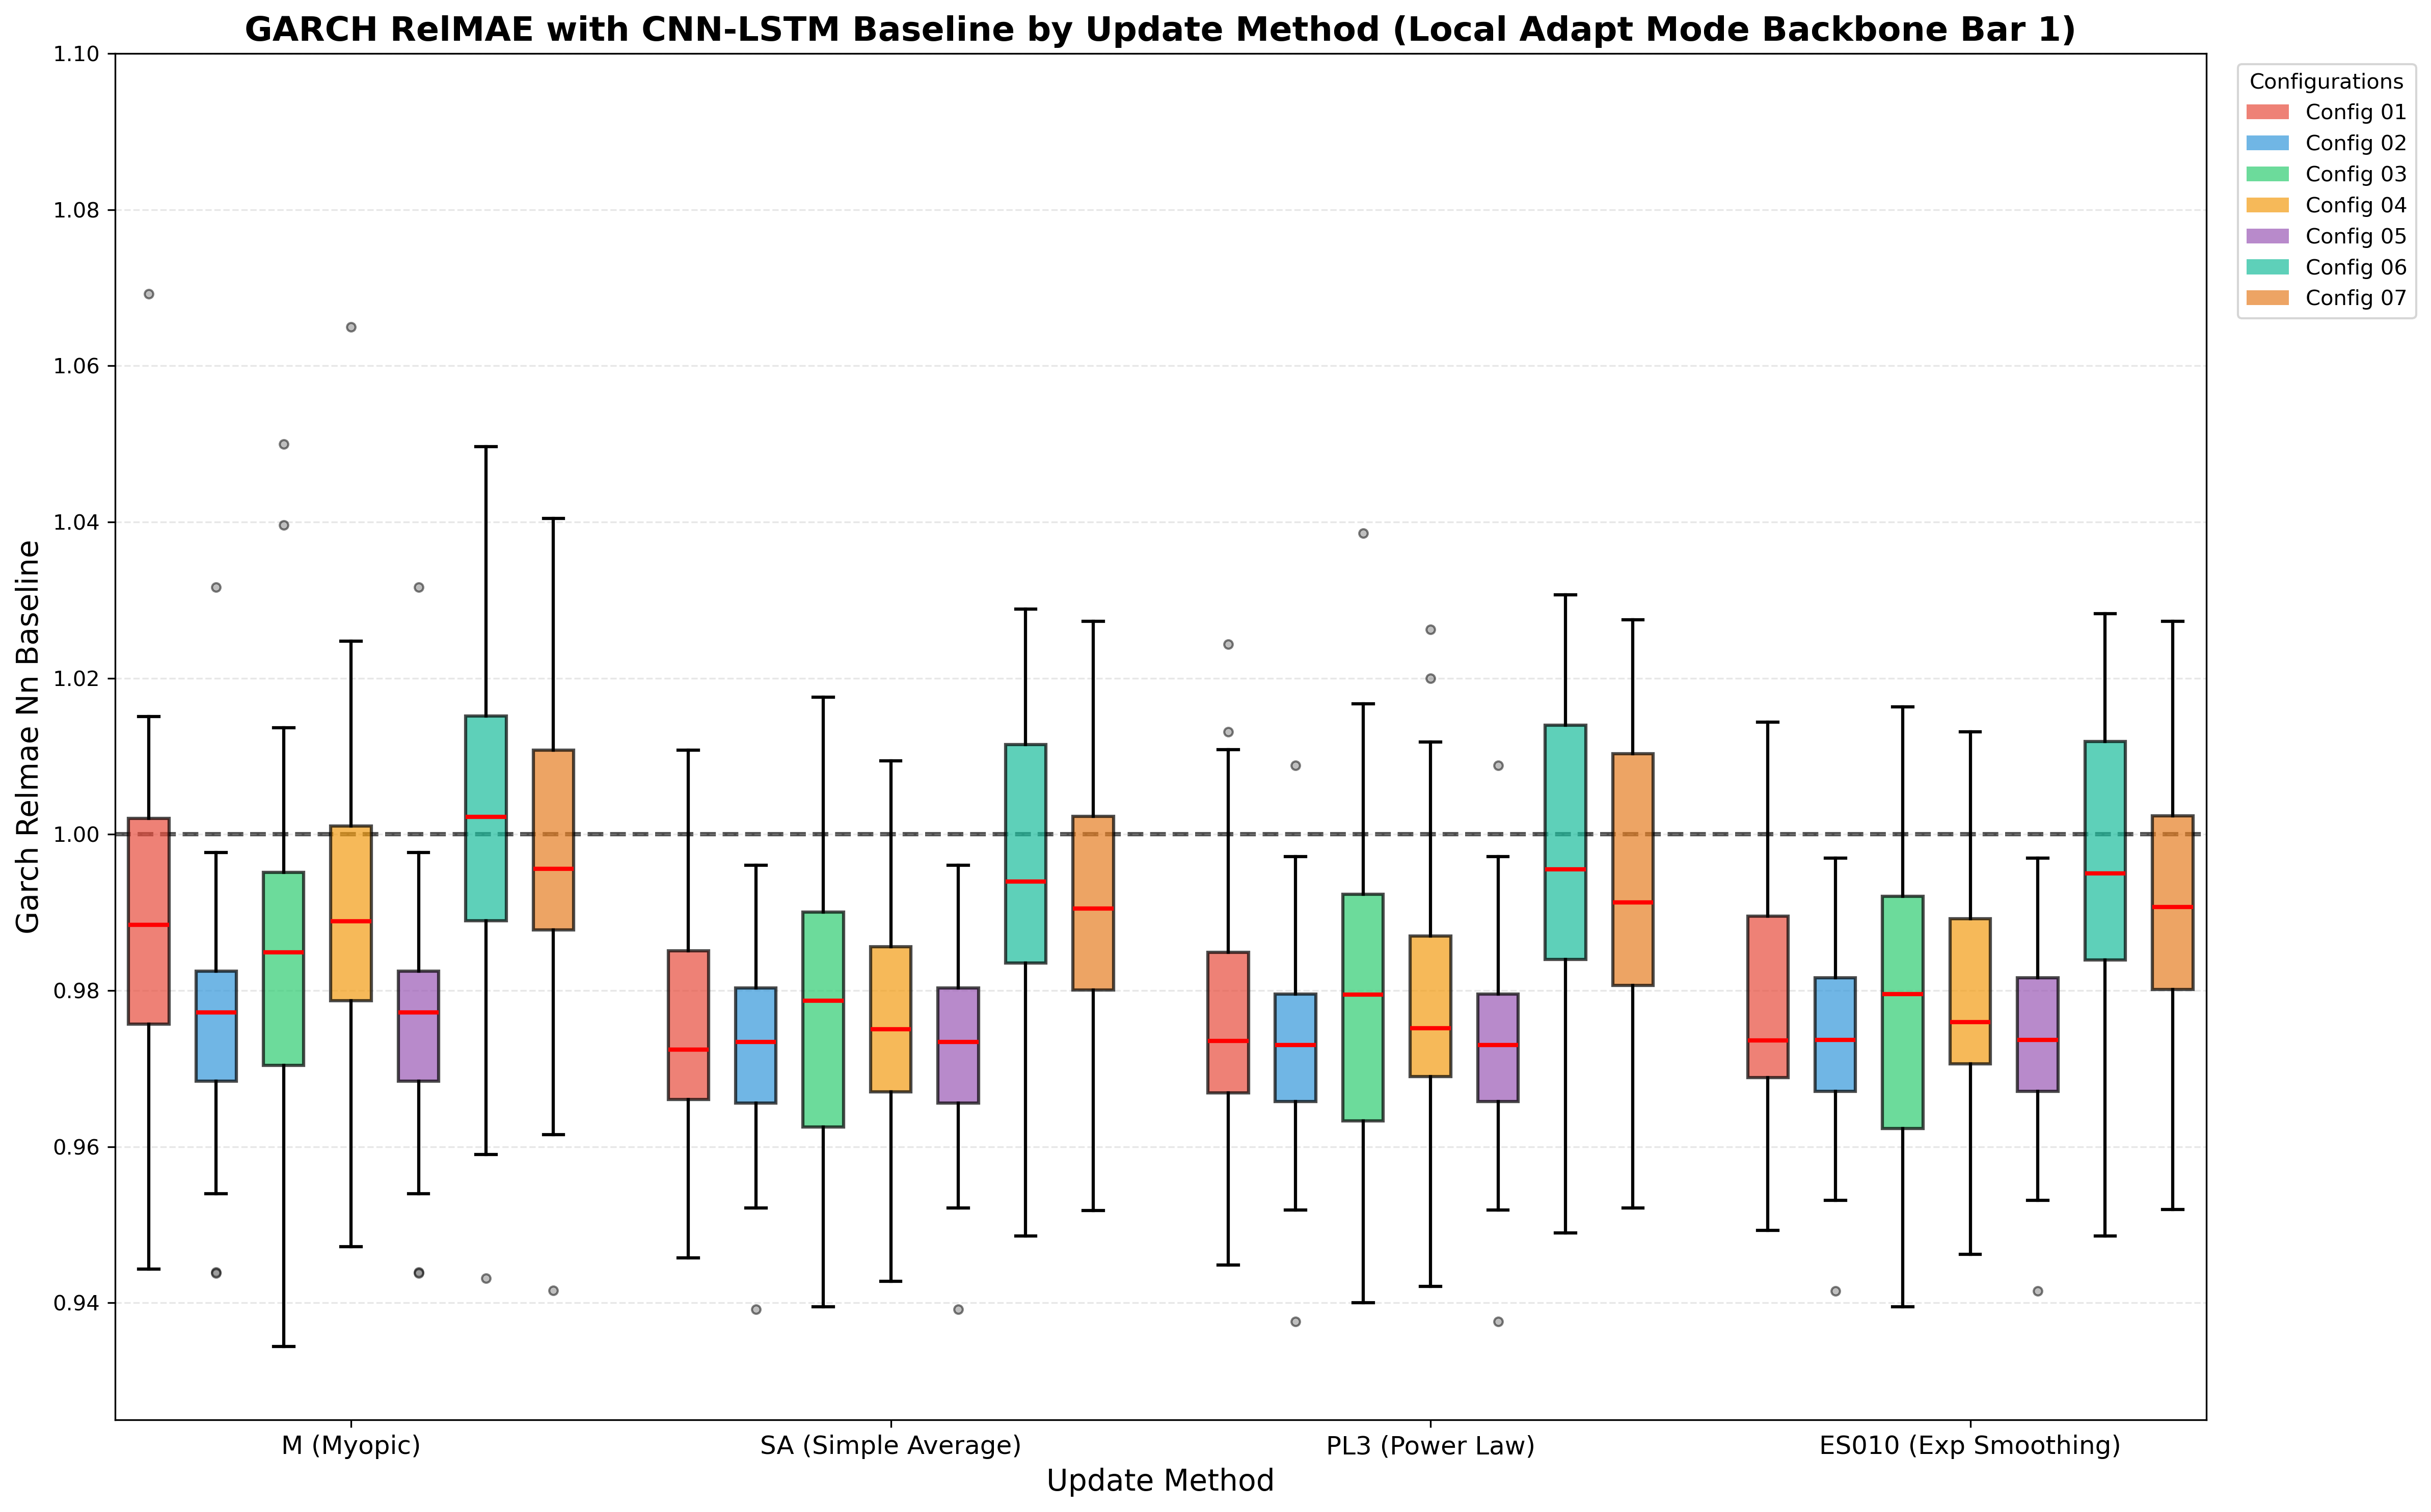
\includegraphics[width=0.85\linewidth]{performance_boxplot_bb000_nn_baseline.png}
\vspace{0.5em}
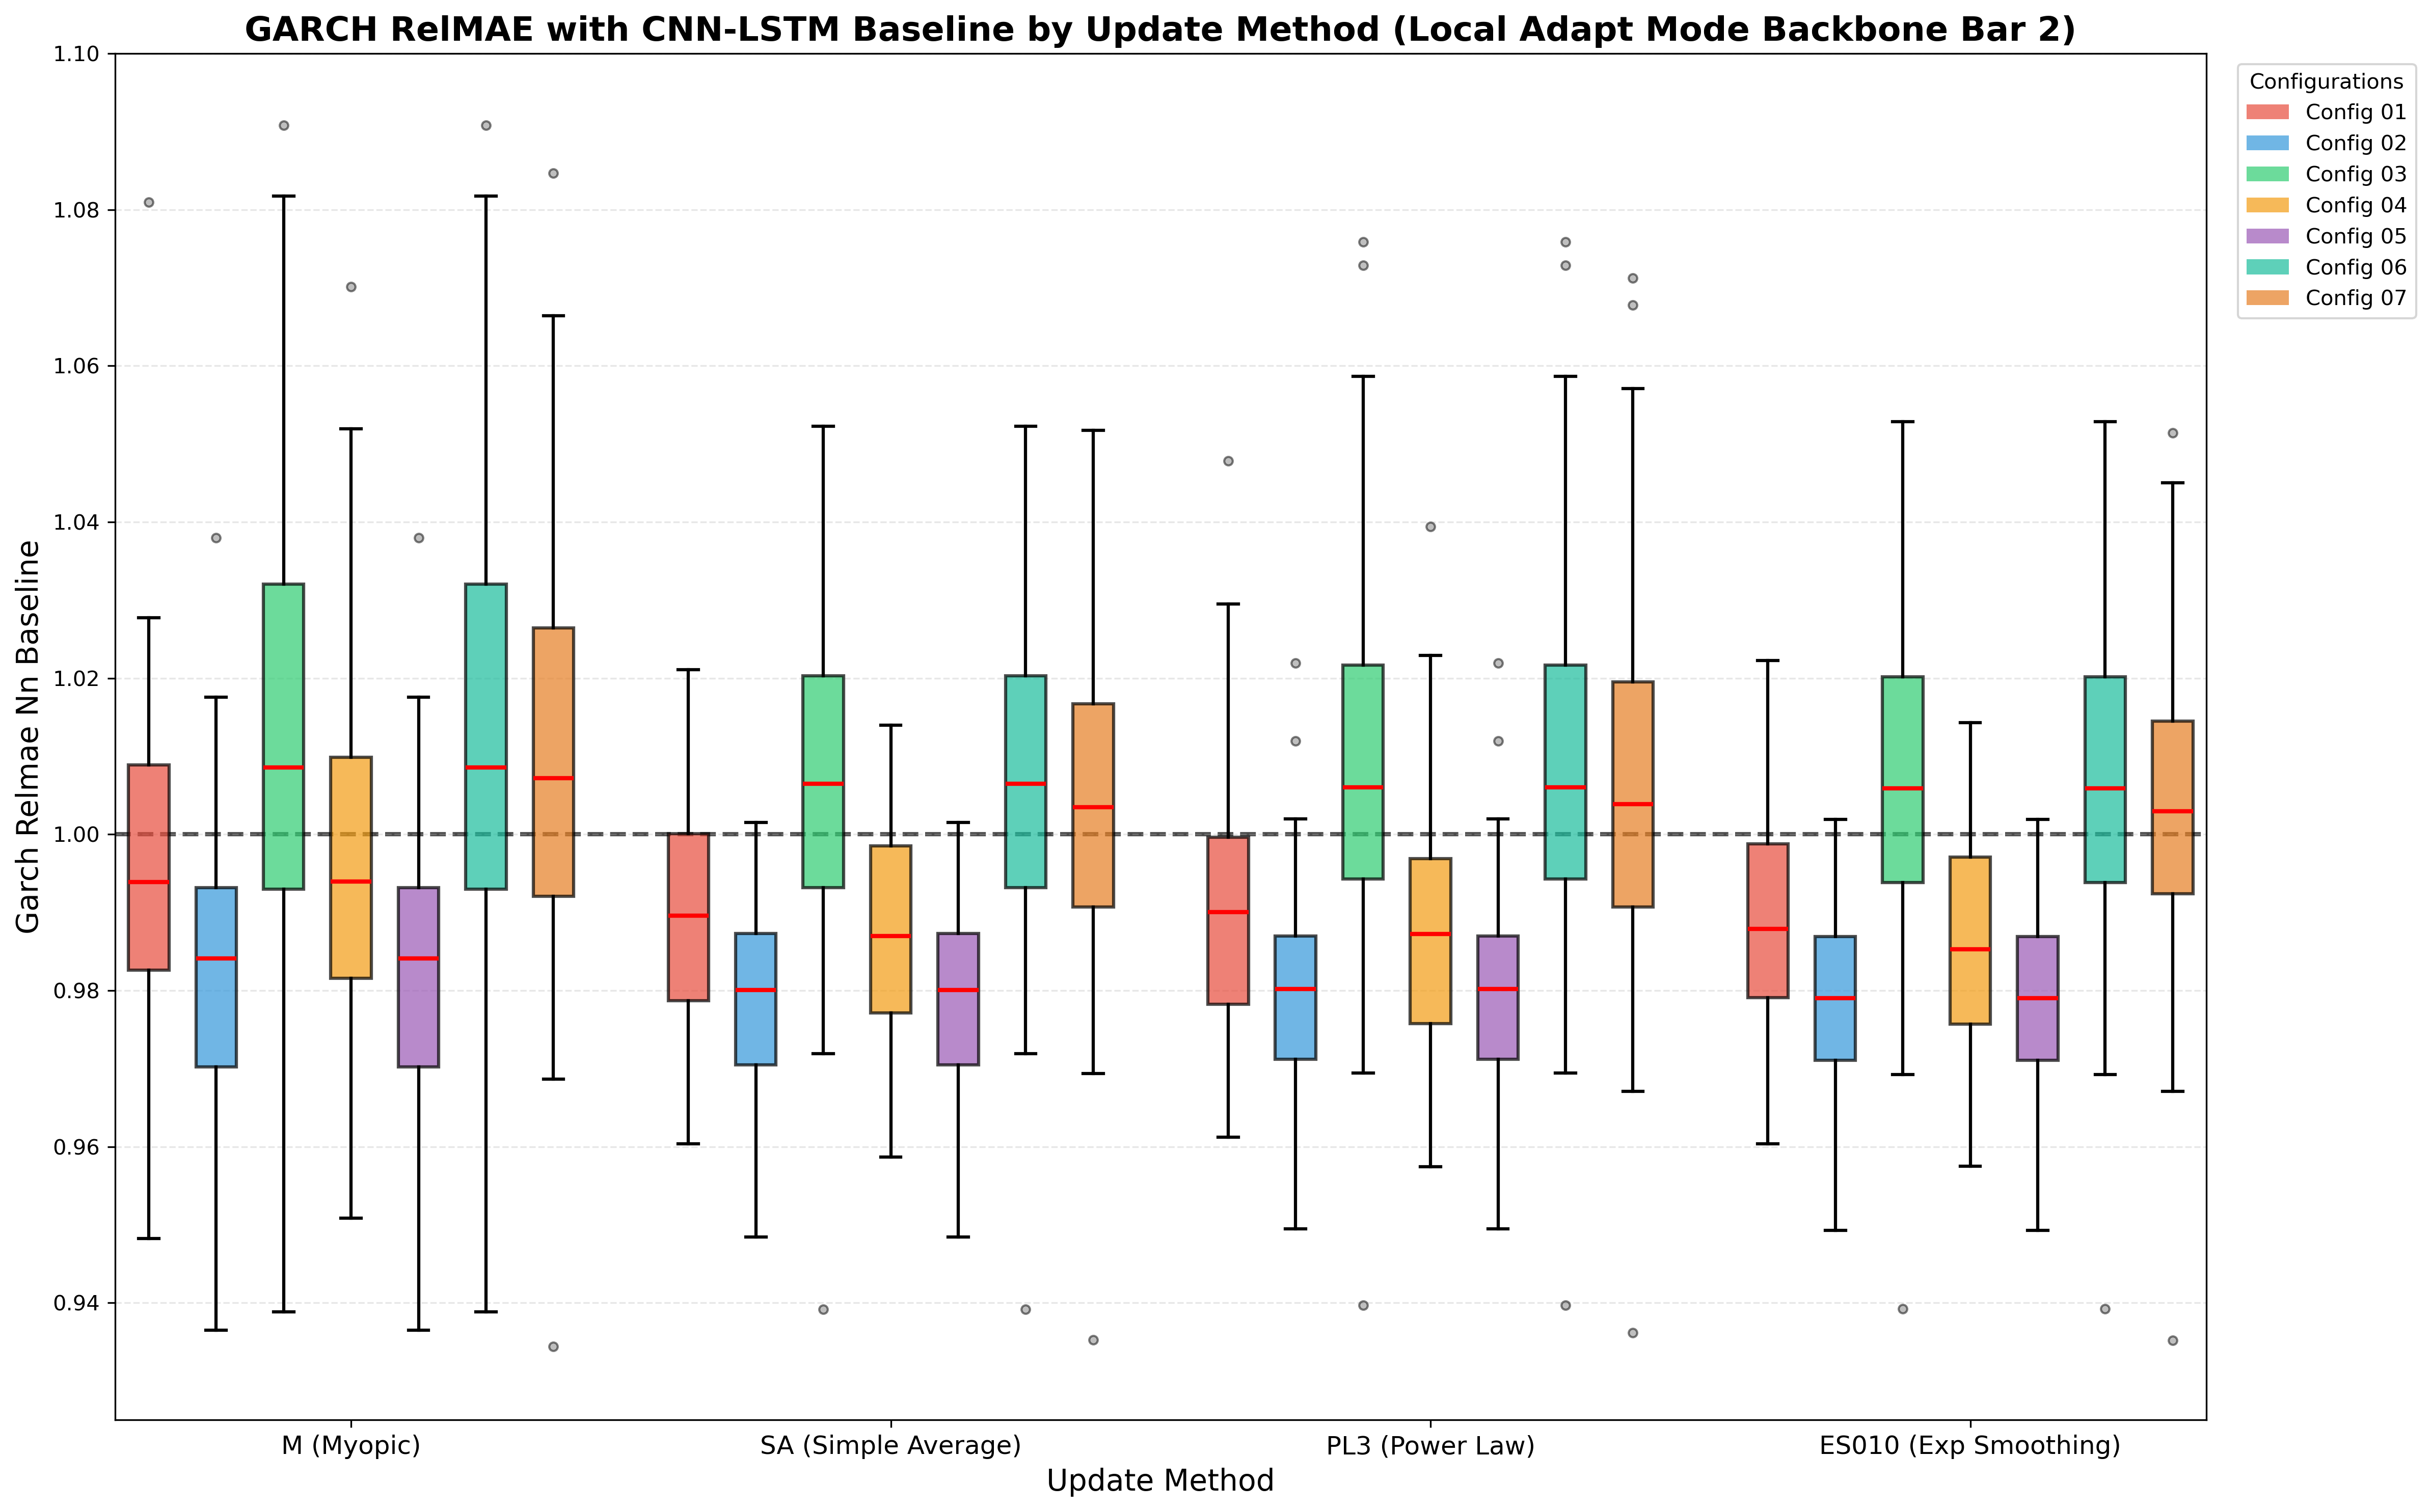
\includegraphics[width=0.85\linewidth]{performance_boxplot_bb001_nn_baseline.png}

\caption{GARCH RelMAE comparison across update methods and configurations with CNN-LSTM baseline.}
\label{fig:garch_relmae_cnn_lstm_baseline_vertical}
\end{figure}


\begin{figure}[htb]
  \centering
  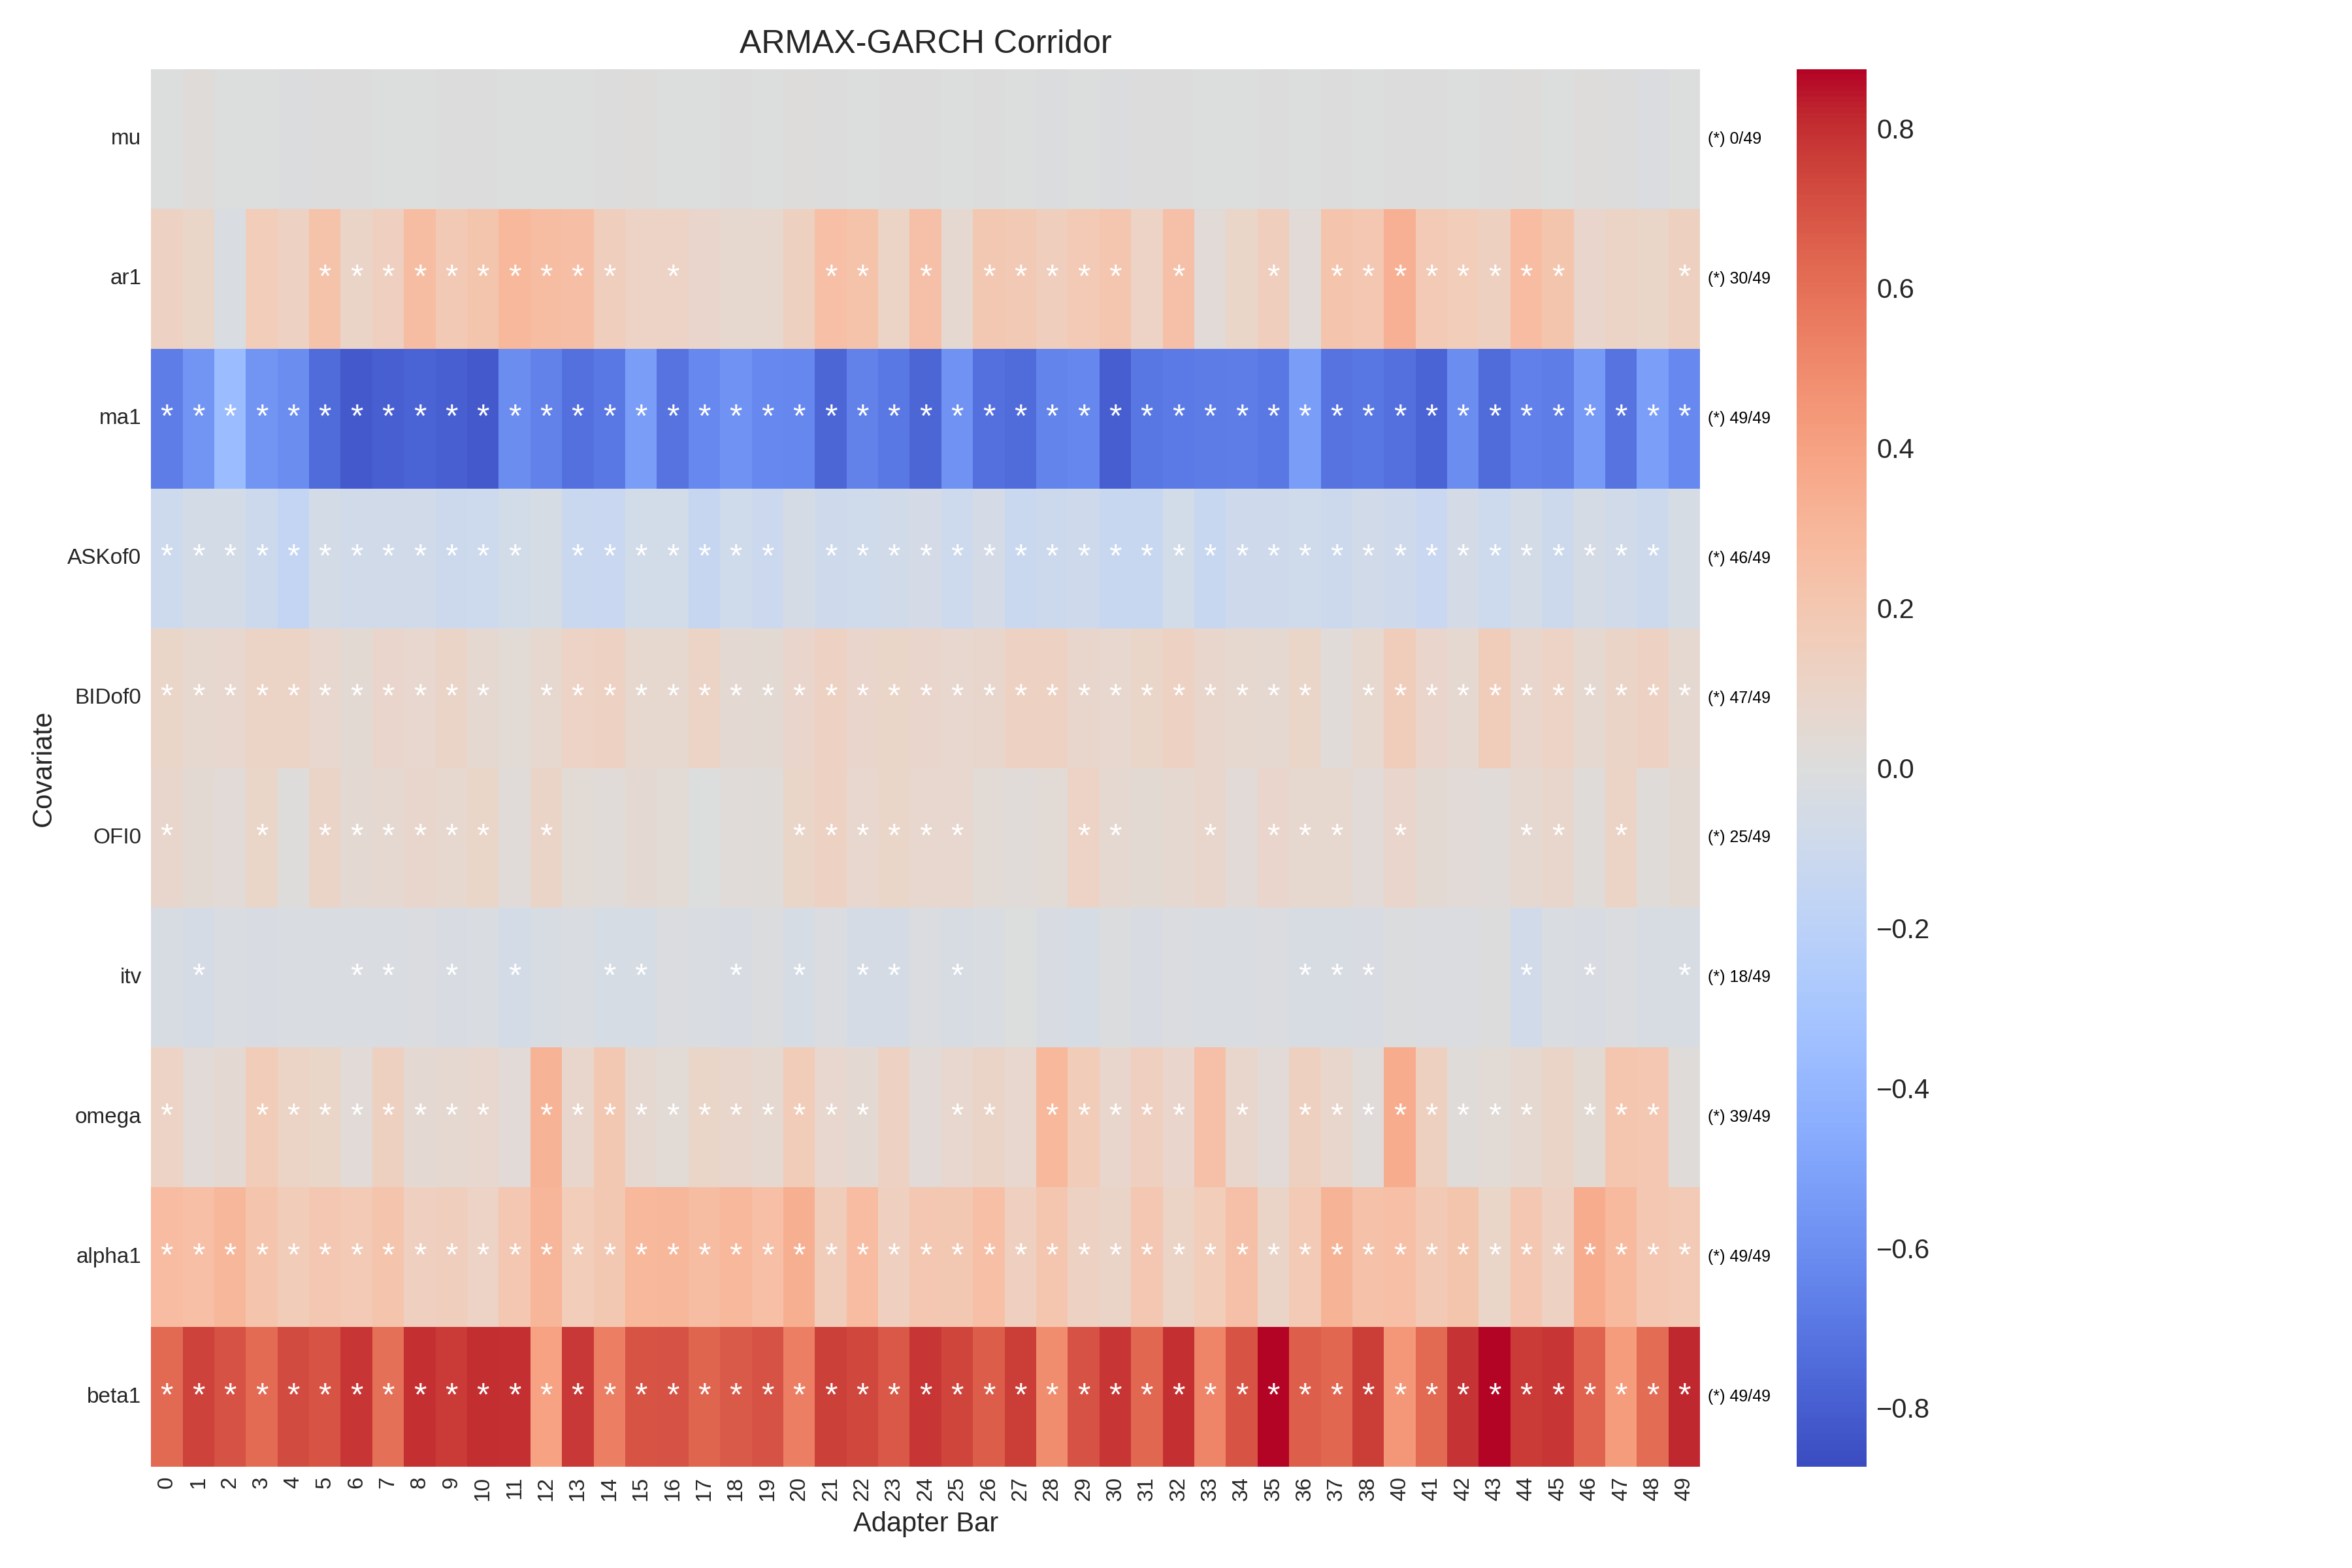
\includegraphics[width=\linewidth]{armax_garch_corridor_SA_03_synthetic_data.png}
  \caption{ARMAX–GARCH-DeepLOB corridor for configuration \texttt{SA\_03}. Cells show bar-specific coefficient magnitudes by adapter bar; asterisks mark statistical significance.}
  \label{fig:armax_garch_corridor_sa_03}
\end{figure}

\begin{figure}[htb]
  \centering
  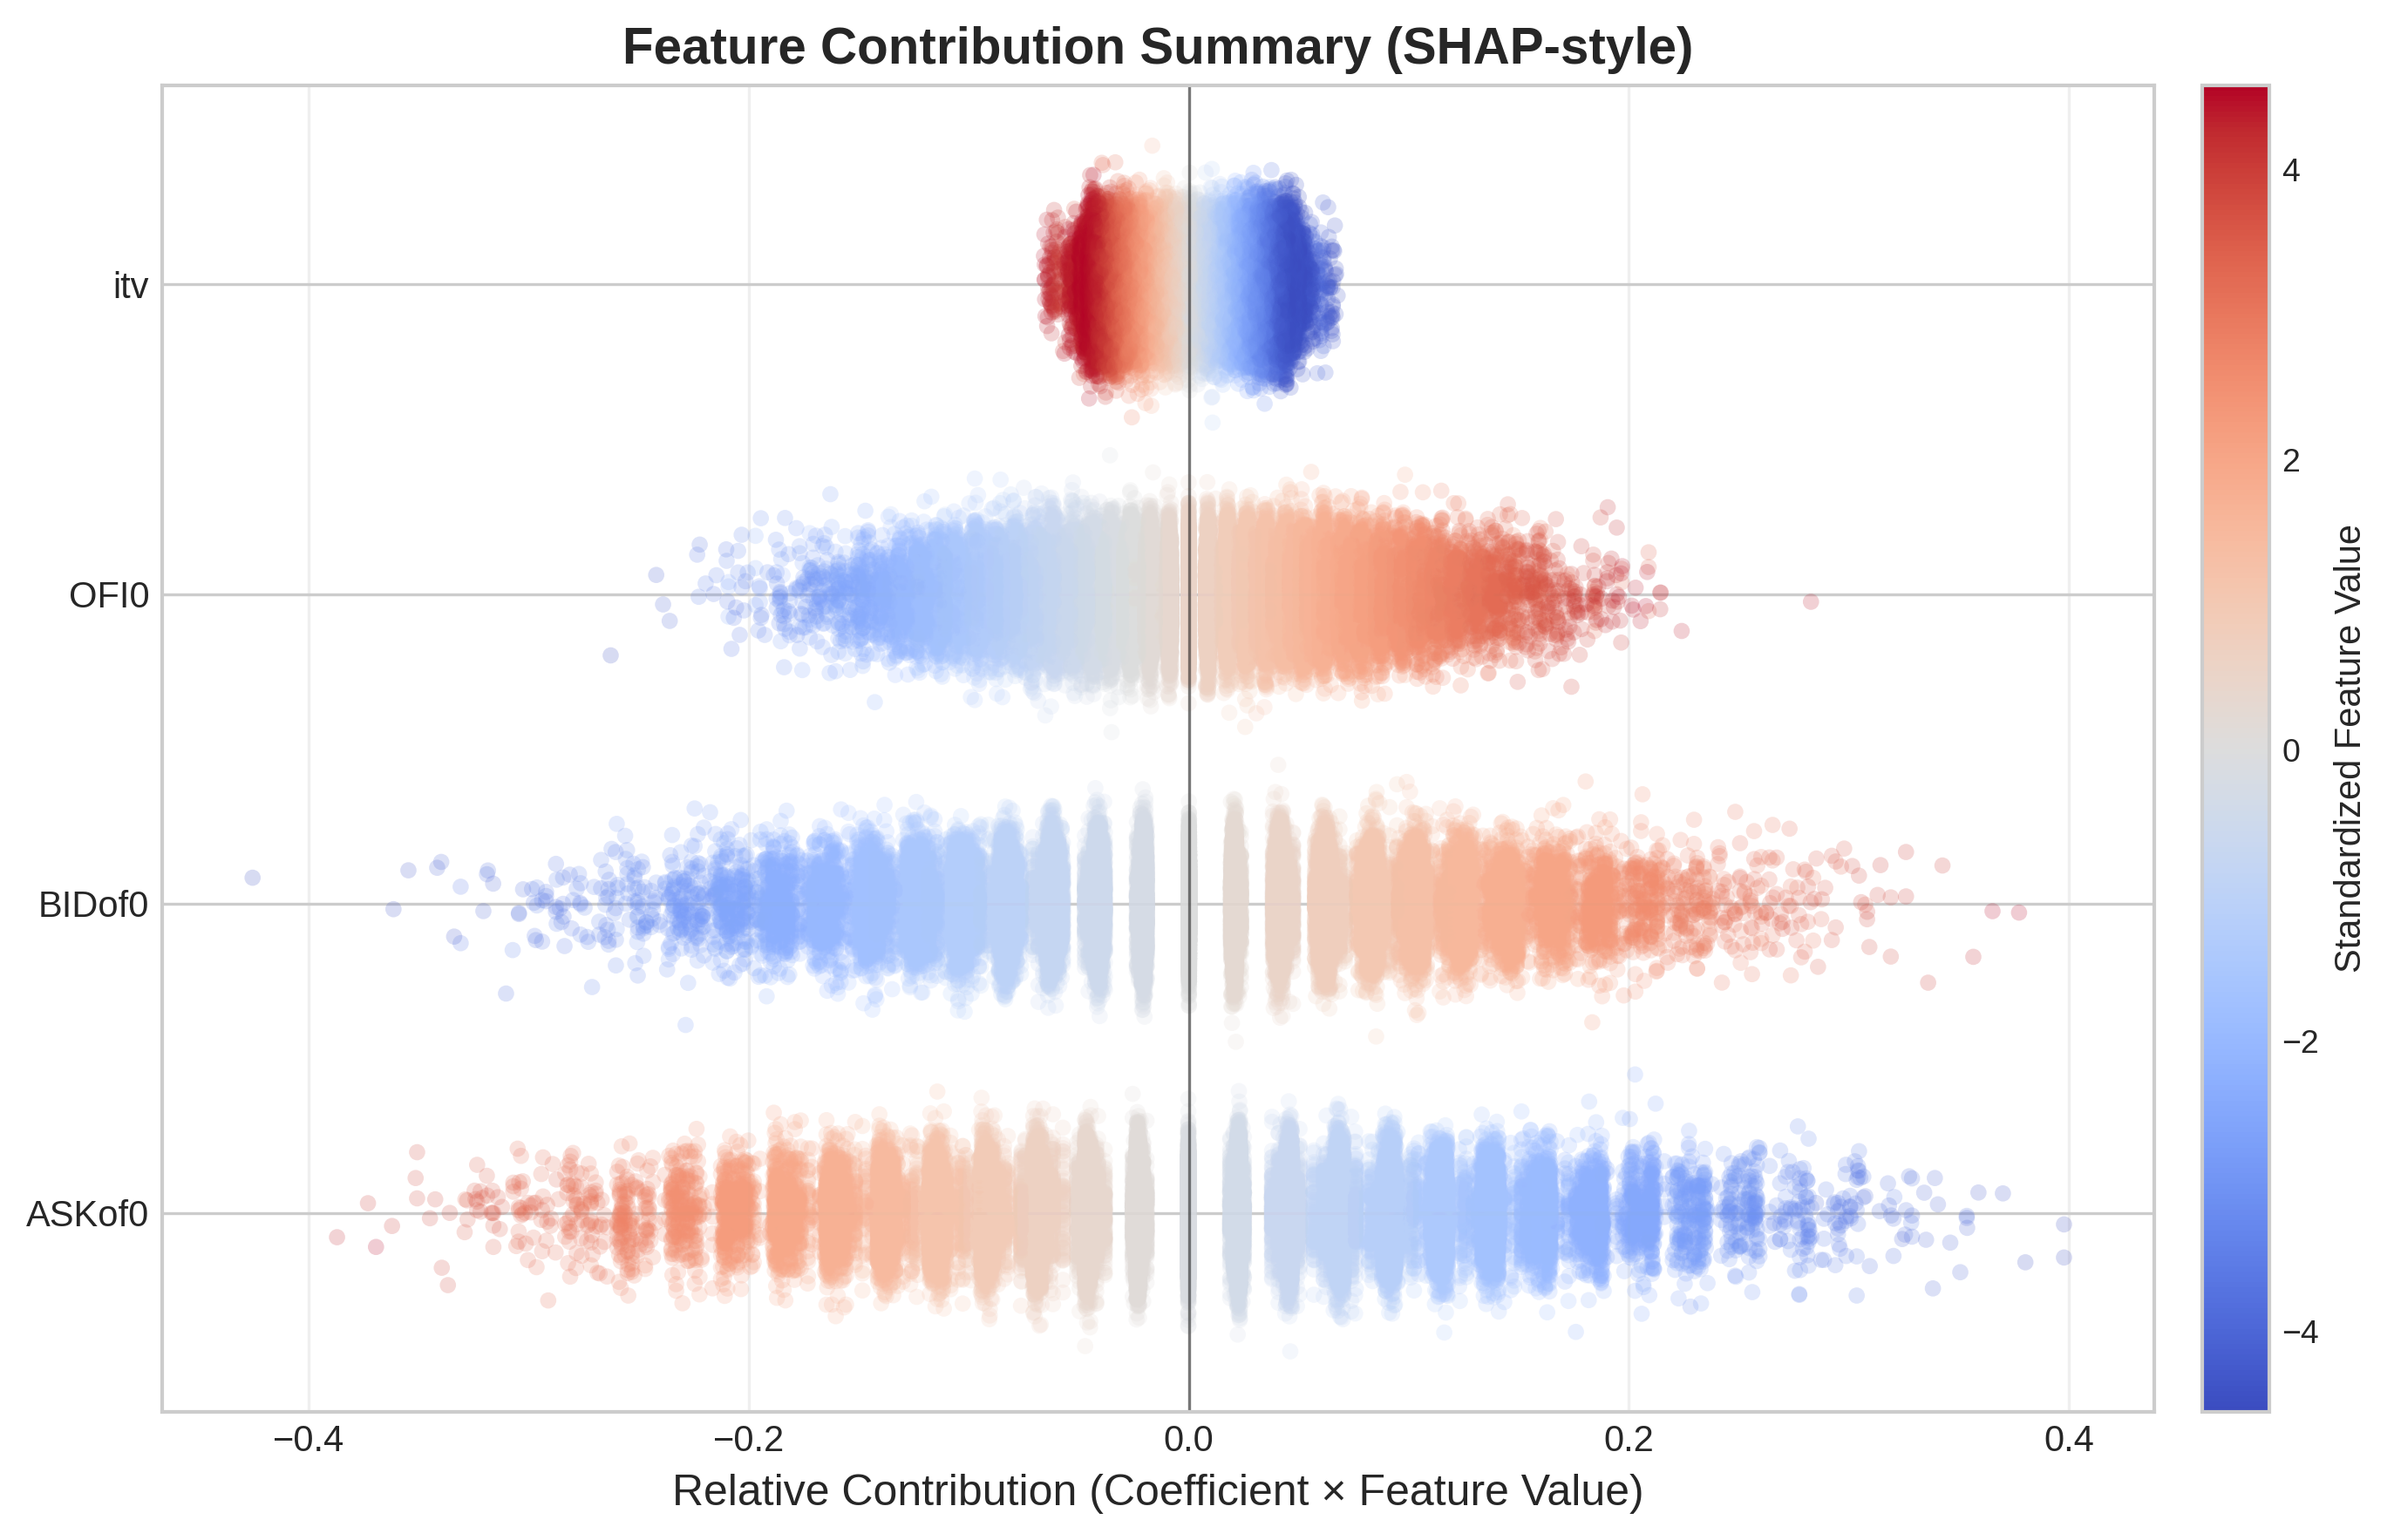
\includegraphics[width=\linewidth]{shap_summary_SA_03_synthetic_data.png}
  \caption{ARMAX–GARCH-DeepLOB SHAP scores \texttt{SA\_03}. The figure plots the product of the coefficient and the feature value for each sample.}
  \label{fig:shap_scores_sa_03}
\end{figure}

\begin{figure}[htb]
  \centering
  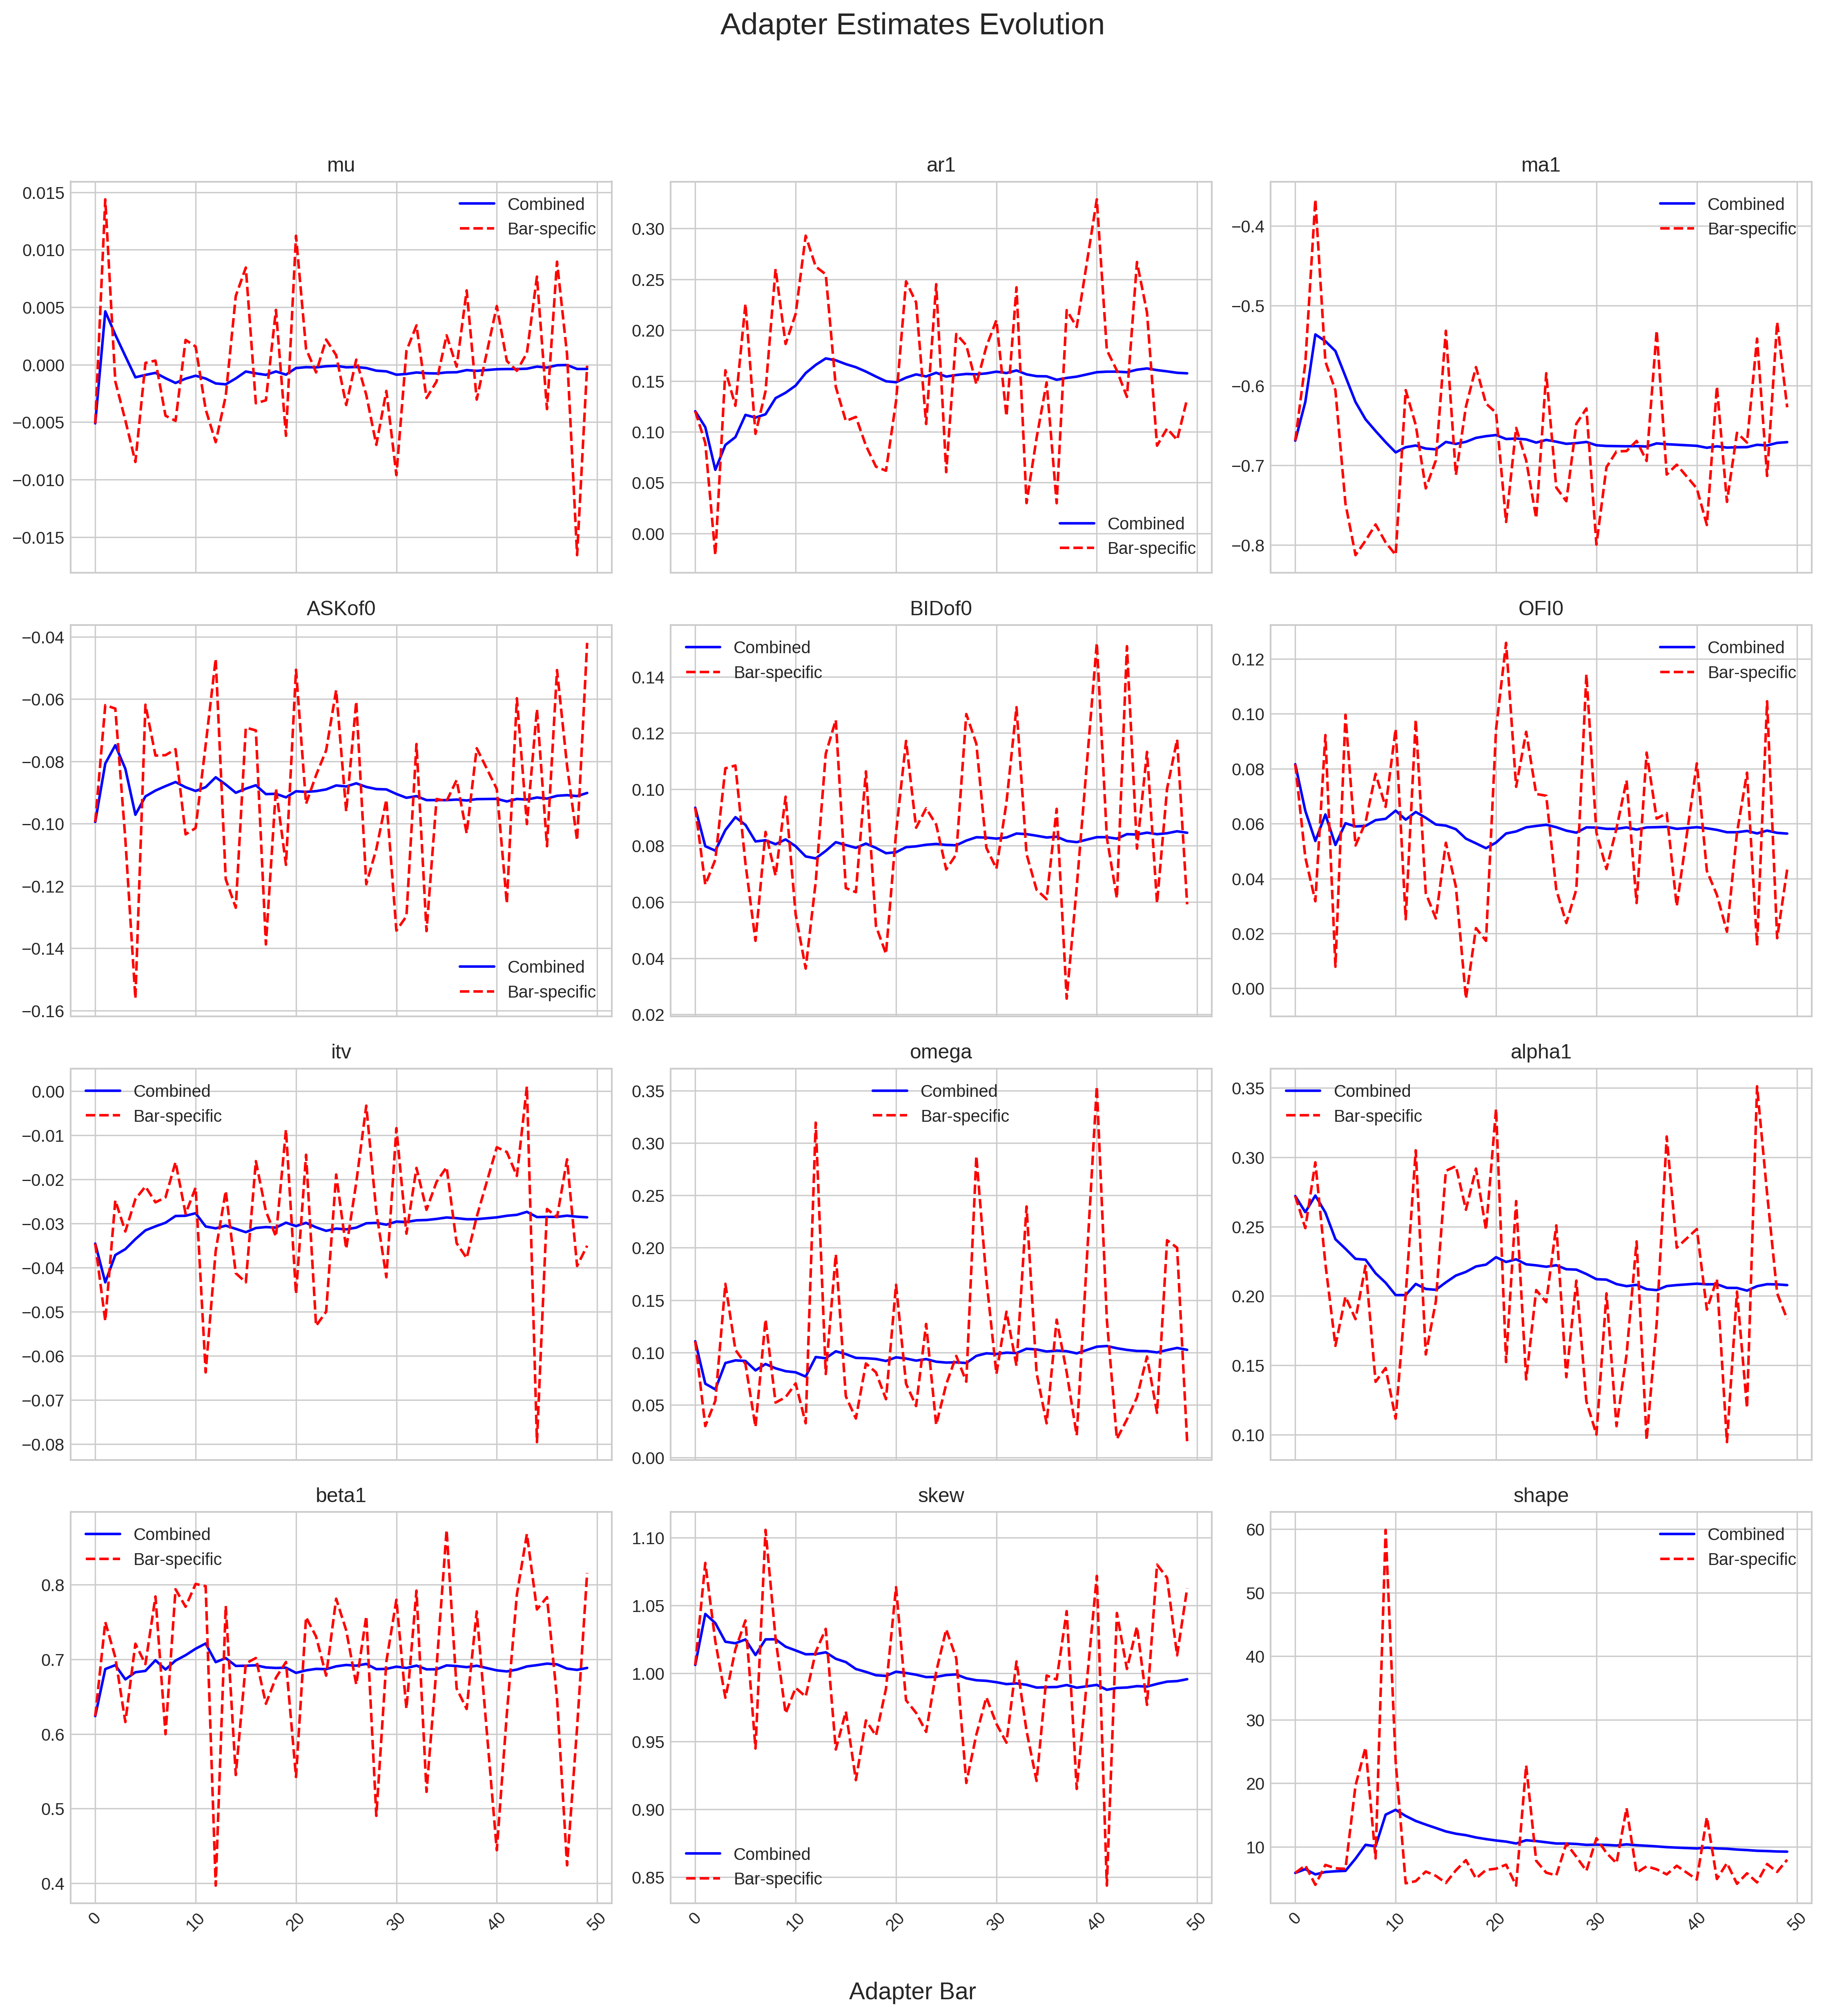
\includegraphics[width=\linewidth]{param_series_SA_03_synthetic_data.png}
  \caption{Evolution of parameter estimates for configuration \texttt{SA\_03}. Blue lines denote combined estimates, while red dashed lines denote bar-specific estimates across adapter bars.}
  \label{fig:param_series_sa_03}
\end{figure}


\begin{longtable}{@{}lll@{}}
\caption{Base configuration used in the experiments with market data.} 
\label{tab:base_config_market_data} \\
\toprule
\textbf{Category} & \textbf{Parameter} & \textbf{Value} \\ \midrule
\endfirsthead

\multicolumn{3}{c}%
{{\bfseries Table \thetable\ (continued)}} \\
\toprule
\textbf{Category} & \textbf{Parameter} & \textbf{Value} \\ \midrule
\endhead

\bottomrule
\endfoot

\multirow{8}{*}{General} 
 & Ticker & INTC \\
 & $\Delta^B$ & $7{,}200.0$ sec \\
 & $\Delta^A$ & $600.0$ sec \\
 & $\delta$ & $2.0$ sec \\
 & Seed & One per date pair \\
 & Session start & 9:45 AM EST \\
 & Session finish & 3:45 PM EST \\
 & Target Variable & $r^w$ \\ \midrule

\multirow{10}{*}{Backbone} 
 & Training Epochs & 10 \\
 & Batch size & 32 \\
 & Validation proportion & 0.1 \\
 & Buffer proportion & 0.05 \\
 & Windsorization quantile & 0.005 \\
 & ADF rejection threshold & 0.8 \\
 & KPSS verification threshold & 0.2 \\
 & NA threshold & 0.2 \\
 & Learning rate & 0.0001 \\
 & Correlation threshold & 0.95 \\ \midrule

\multirow{9}{*}{Interface} 
 & $\alpha$  & \{0.0, 0.1, 0.25, 0.5, 0.75, 0.9, 1.0\} \\
 & $\lambda_1$ & $\mathrm{logspace}(-4,1,25)$ \\
 & $\tau$   & \{0.25, 0.5, 1.0, 1.5, 2.0\} \\
 & $\lambda_2$ & $\mathrm{logspace}(0,1,25)$ \\
 & Validation proportion & 0.2 \\
 & Selection threshold & 0.29 ($L = 12$, $\alpha = 0.00005$) \\
 & Tolerance threshold & $10^{-6}$ \\
 & OLS significance level & 0.05 \\
 & Surrogate model lags & 5 \\ \midrule

\multirow{3}{*}{Adapter} 
 & ARMA order & (0,1) \\
 & \textbf{EGARCH} order & (1,1) \\
 & Error distribution & Negative Inverse Gaussian \\ 
 & Update Rule & Exponential Smoothing \\
\end{longtable}

% Add this to your preamble:
% \usepackage{longtable}

\begingroup
\small % Reduces font size slightly to ensure width fits
\setlength{\tabcolsep}{3pt} % Reduces space between columns
\begin{longtable}{@{}ccccccccc@{}}

% --- CAPTION AND LABEL ---
\caption{RelMAE-based overall rankings and average RelMAE values for each TTSTL configuration across the backbone bars in the INTC MBO dataset. DP denotes the date pair, UR the update rule, CC the covariate configuration, Rank BBX the overall ranking within backbone bar X, and RelMAE BBX the corresponding average forecasting error.} 
\label{tab:intc_data_results} \\

% --- HEADER FOR FIRST PAGE ---
\toprule
DP & UR & CC & Rank BB0 & RelMAE BB0 & Rank BB1 & RelMAE BB1 & Rank BB2 & RelMAE BB2 \\
\midrule
\endfirsthead

% --- HEADER FOR SUBSEQUENT PAGES ---
\multicolumn{9}{c}{{\bfseries \tablename\ \thetable{} -- continued from previous page}} \\
\toprule
DP & UR & CC & Rank BB0 & RelMAE BB1 & Rank BB1 & RelMAE BB2 & Rank BB3 & RelMAE BB2 \\
\midrule
\endhead

% --- FOOTER FOR BOTTOM OF PAGES ---
\midrule
\multicolumn{9}{r}{{Continued on next page}} \\
\bottomrule
\endfoot

% --- FOOTER FOR LAST PAGE ---
\bottomrule
\endlastfoot

% --- DATA CONTENT ---
1 & ES010 & 01 & 3.0 & 99.98\% & 3.0 & 100.63\% & 3.0 & 99.17\% \\
1 & ES010 & 02 & 3.0 & 99.98\% & 3.0 & 100.63\% & 3.0 & 99.17\% \\
1 & ES010 & 03 & 3.0 & 99.98\% & 3.0 & 100.63\% & 3.0 & 99.17\% \\
1 & ES010 & 04 & 3.0 & 99.98\% & 3.0 & 100.63\% & 3.0 & 99.17\% \\
1 & ES010 & 05 & 6.0 & 100.02\% & 6.0 & 100.75\% & 6.0 & 99.20\% \\
1 & ES010 & 06 & 3.0 & 99.98\% & 3.0 & 100.63\% & 3.0 & 99.17\% \\
2 & ES010 & 01 & 3.0 & 99.84\% & 3.0 & 100.56\% & 4.0 & 100.39\% \\
2 & ES010 & 02 & 3.0 & 99.84\% & 3.0 & 100.56\% & 4.0 & 100.39\% \\
2 & ES010 & 03 & 3.0 & 99.84\% & 3.0 & 100.56\% & 4.0 & 100.39\% \\
2 & ES010 & 04 & 3.0 & 99.84\% & 3.0 & 100.56\% & 4.0 & 100.39\% \\
2 & ES010 & 05 & 6.0 & 100.43\% & 6.0 & 100.75\% & 1.0 & 100.32\% \\
2 & ES010 & 06 & 3.0 & 99.84\% & 3.0 & 100.56\% & 4.0 & 100.39\% \\
3 & ES010 & 01 & 3.0 & 99.85\% & 3.0 & 100.17\% & 2.5 & 100.53\% \\
3 & ES010 & 02 & 3.0 & 99.85\% & 3.0 & 100.17\% & 5.5 & 100.59\% \\
3 & ES010 & 03 & 3.0 & 99.85\% & 3.0 & 100.17\% & 2.5 & 100.53\% \\
3 & ES010 & 04 & 3.0 & 99.85\% & 3.0 & 100.17\% & 2.5 & 100.53\% \\
3 & ES010 & 05 & 6.0 & 99.91\% & 6.0 & 100.32\% & 5.5 & 100.59\% \\
3 & ES010 & 06 & 3.0 & 99.85\% & 3.0 & 100.17\% & 2.5 & 100.53\% \\
4 & ES010 & 01 & 3.0 & 99.64\% & 4.5 & 102.53\% & 4.0 & 101.48\% \\
4 & ES010 & 02 & 3.0 & 99.64\% & 1.5 & 101.04\% & 4.0 & 101.48\% \\
4 & ES010 & 03 & 3.0 & 99.64\% & 4.5 & 102.53\% & 4.0 & 101.48\% \\
4 & ES010 & 04 & 3.0 & 99.64\% & 4.5 & 102.53\% & 4.0 & 101.48\% \\
4 & ES010 & 05 & 6.0 & 100.45\% & 1.5 & 101.04\% & 1.0 & 101.38\% \\
4 & ES010 & 06 & 3.0 & 99.64\% & 4.5 & 102.53\% & 4.0 & 101.48\% \\
5 & ES010 & 01 & 3.0 & 99.93\% & 4.5 & 99.80\% & 4.0 & 99.77\% \\
5 & ES010 & 02 & 3.0 & 99.93\% & 1.5 & 99.76\% & 4.0 & 99.77\% \\
5 & ES010 & 03 & 3.0 & 99.93\% & 4.5 & 99.80\% & 4.0 & 99.77\% \\
5 & ES010 & 04 & 3.0 & 99.93\% & 4.5 & 99.80\% & 4.0 & 99.77\% \\
5 & ES010 & 05 & 6.0 & 100.06\% & 1.5 & 99.76\% & 1.0 & 99.77\% \\
5 & ES010 & 06 & 3.0 & 99.93\% & 4.5 & 99.80\% & 4.0 & 99.77\% \\
6 & ES010 & 01 & 4.0 & 100.40\% & 3.5 & 102.23\% & 2.5 & 100.14\% \\
6 & ES010 & 02 & 4.0 & 100.40\% & 5.5 & 131.02\% & 5.5 & 127.17\% \\
6 & ES010 & 03 & 4.0 & 100.40\% & 1.5 & 100.67\% & 2.5 & 100.14\% \\
6 & ES010 & 04 & 4.0 & 100.40\% & 3.5 & 102.23\% & 2.5 & 100.14\% \\
6 & ES010 & 05 & 1.0 & 100.36\% & 5.5 & 131.02\% & 5.5 & 127.17\% \\
6 & ES010 & 06 & 4.0 & 100.40\% & 1.5 & 100.67\% & 2.5 & 100.14\% \\
7 & ES010 & 01 & 3.0 & 99.99\% & 2.5 & 99.00\% & 3.0 & 99.26\% \\
7 & ES010 & 02 & 3.0 & 99.99\% & 5.5 & 112.60\% & 3.0 & 99.26\% \\
7 & ES010 & 03 & 3.0 & 99.99\% & 2.5 & 99.00\% & 3.0 & 99.26\% \\
7 & ES010 & 04 & 3.0 & 99.99\% & 2.5 & 99.00\% & 3.0 & 99.26\% \\
7 & ES010 & 05 & 6.0 & 100.03\% & 5.5 & 112.60\% & 6.0 & 99.27\% \\
7 & ES010 & 06 & 3.0 & 99.99\% & 2.5 & 99.00\% & 3.0 & 99.26\% \\
8 & ES010 & 01 & 3.0 & 98.15\% & 4.0 & 101.29\% & 3.0 & 100.14\% \\
8 & ES010 & 02 & 3.0 & 98.15\% & 4.0 & 101.29\% & 3.0 & 100.14\% \\
8 & ES010 & 03 & 3.0 & 98.15\% & 4.0 & 101.29\% & 3.0 & 100.14\% \\
8 & ES010 & 04 & 3.0 & 98.15\% & 4.0 & 101.29\% & 3.0 & 100.14\% \\
8 & ES010 & 05 & 6.0 & 98.67\% & 1.0 & 100.88\% & 6.0 & 100.27\% \\
8 & ES010 & 06 & 3.0 & 98.15\% & 4.0 & 101.29\% & 3.0 & 100.14\% \\
9 & ES010 & 01 & 3.0 & 99.77\% & 2.5 & 100.34\% & 2.0 & 100.46\% \\
9 & ES010 & 02 & 3.0 & 99.77\% & 5.5 & 101.93\% & 5.0 & 100.56\% \\
9 & ES010 & 03 & 3.0 & 99.77\% & 2.5 & 100.34\% & 5.0 & 100.56\% \\
9 & ES010 & 04 & 3.0 & 99.77\% & 2.5 & 100.34\% & 1.0 & 100.46\% \\
9 & ES010 & 05 & 6.0 & 99.75\% & 5.5 & 101.93\% & 3.0 & 100.68\% \\
9 & ES010 & 06 & 3.0 & 99.77\% & 2.5 & 100.34\% & 5.0 & 100.56\% \\
10 & ES010 & 01 & 3.0 & 100.33\% & 3.0 & 100.57\% & 3.0 & 99.83\% \\
10 & ES010 & 02 & 3.0 & 100.33\% & 3.0 & 100.57\% & 3.0 & 99.83\% \\
10 & ES010 & 03 & 3.0 & 100.33\% & 3.0 & 100.57\% & 3.0 & 99.83\% \\
10 & ES010 & 04 & 3.0 & 100.33\% & 3.0 & 100.57\% & 3.0 & 99.83\% \\
10 & ES010 & 05 & 6.0 & 100.70\% & 6.0 & 100.59\% & 6.0 & 99.88\% \\
10 & ES010 & 06 & 3.0 & 100.33\% & 3.0 & 100.57\% & 3.0 & 99.83\% \\
\end{longtable}
\endgroup

\begin{figure}[ht!]
\centering

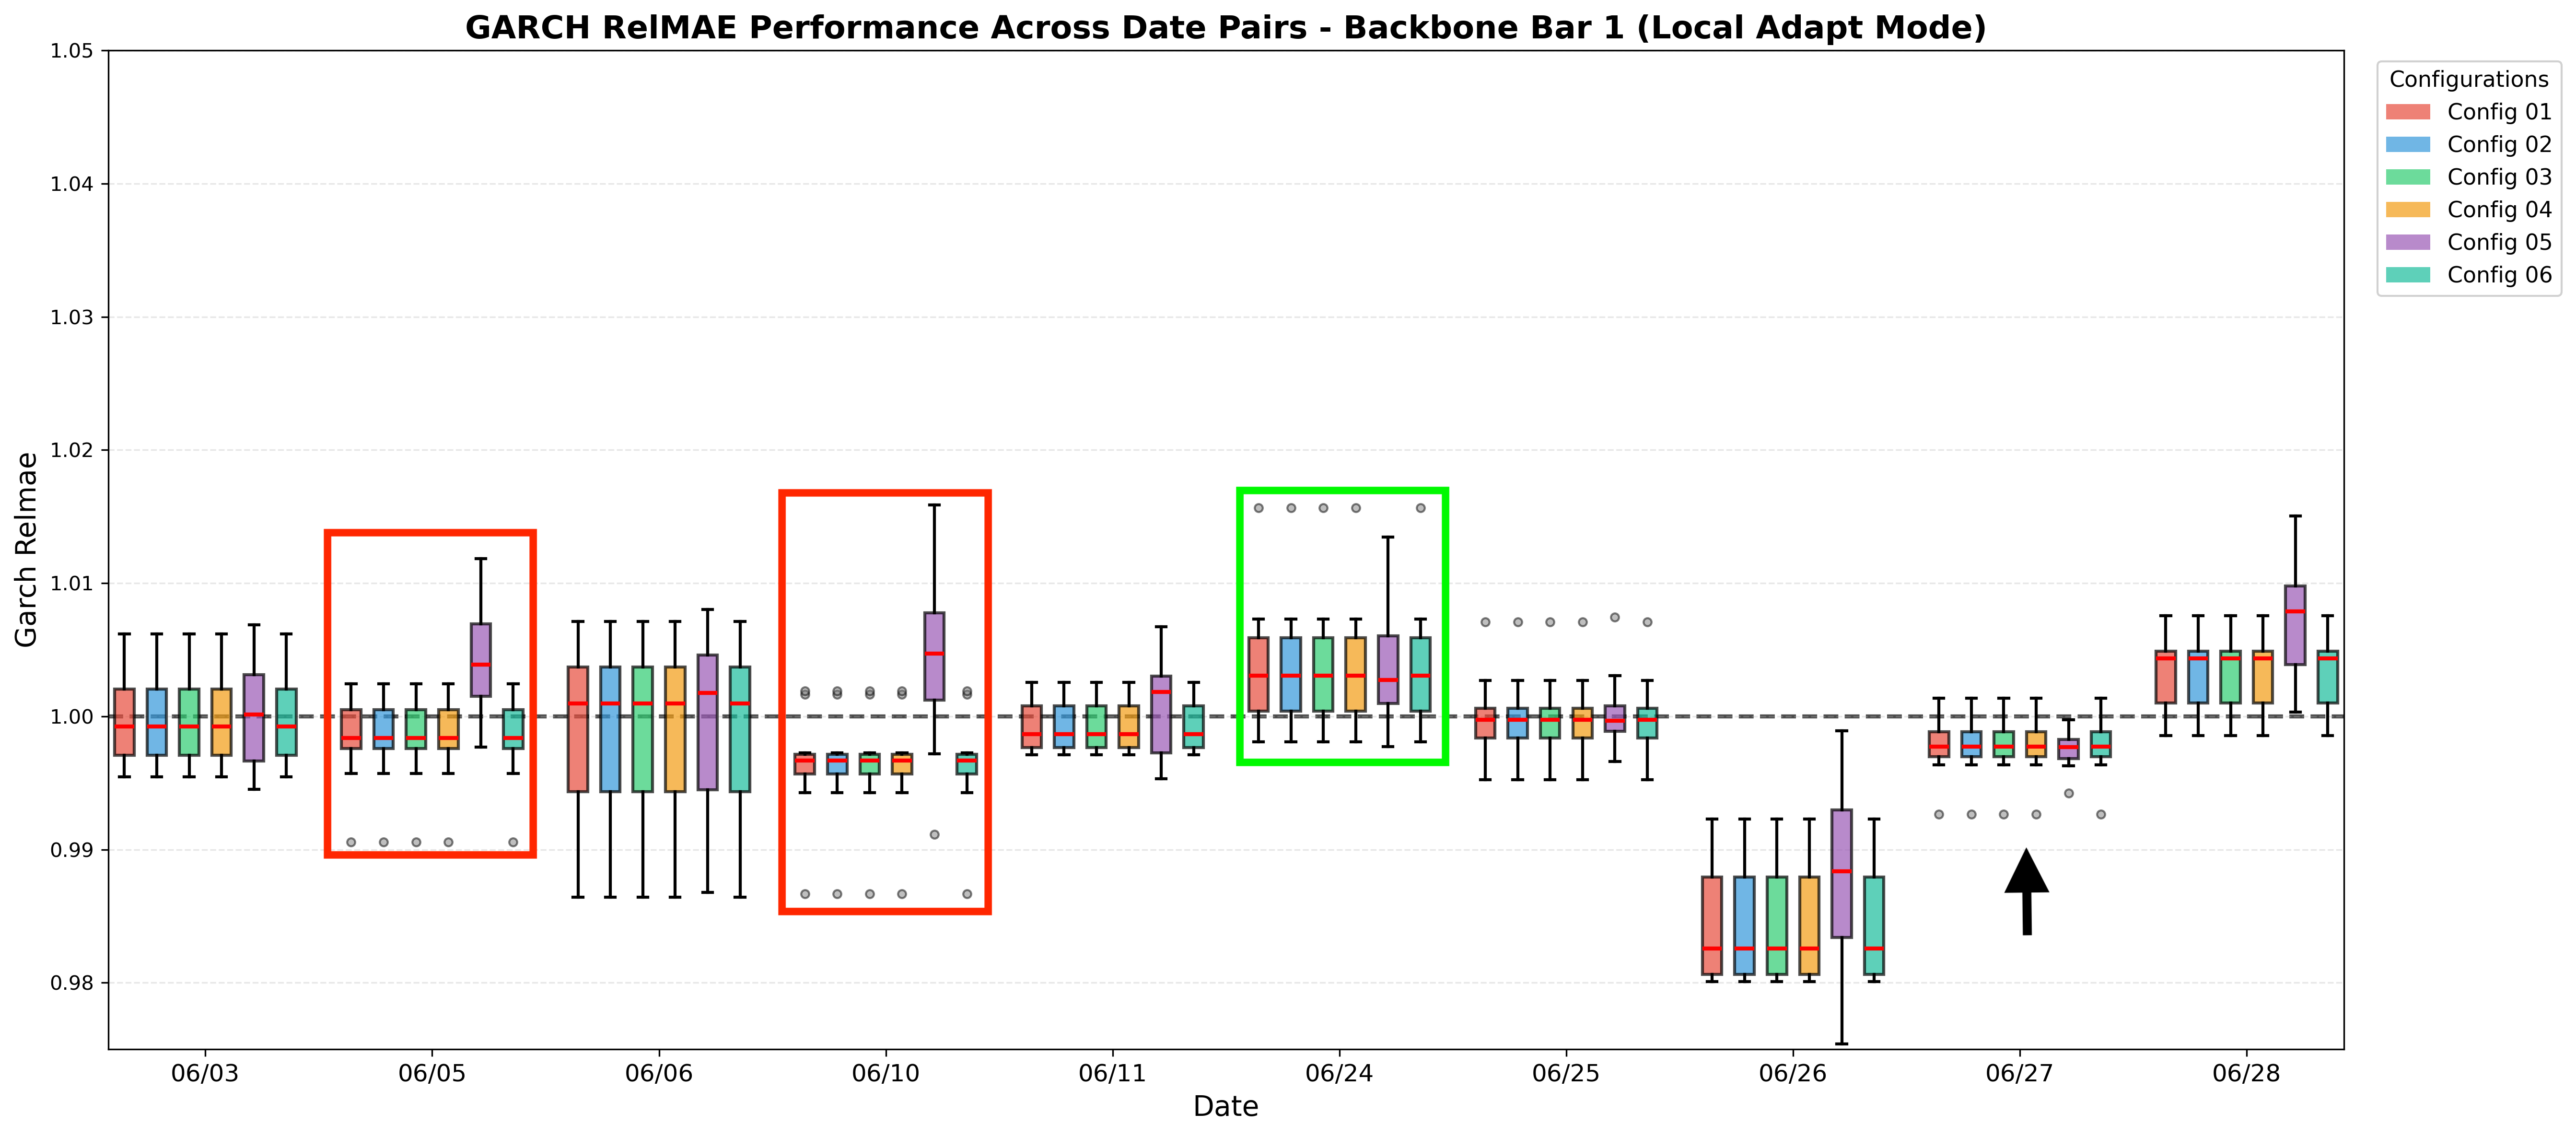
\includegraphics[width=0.9\linewidth]{sequential_boxplot_bb_000_marked.png}
\vspace{0.5em}
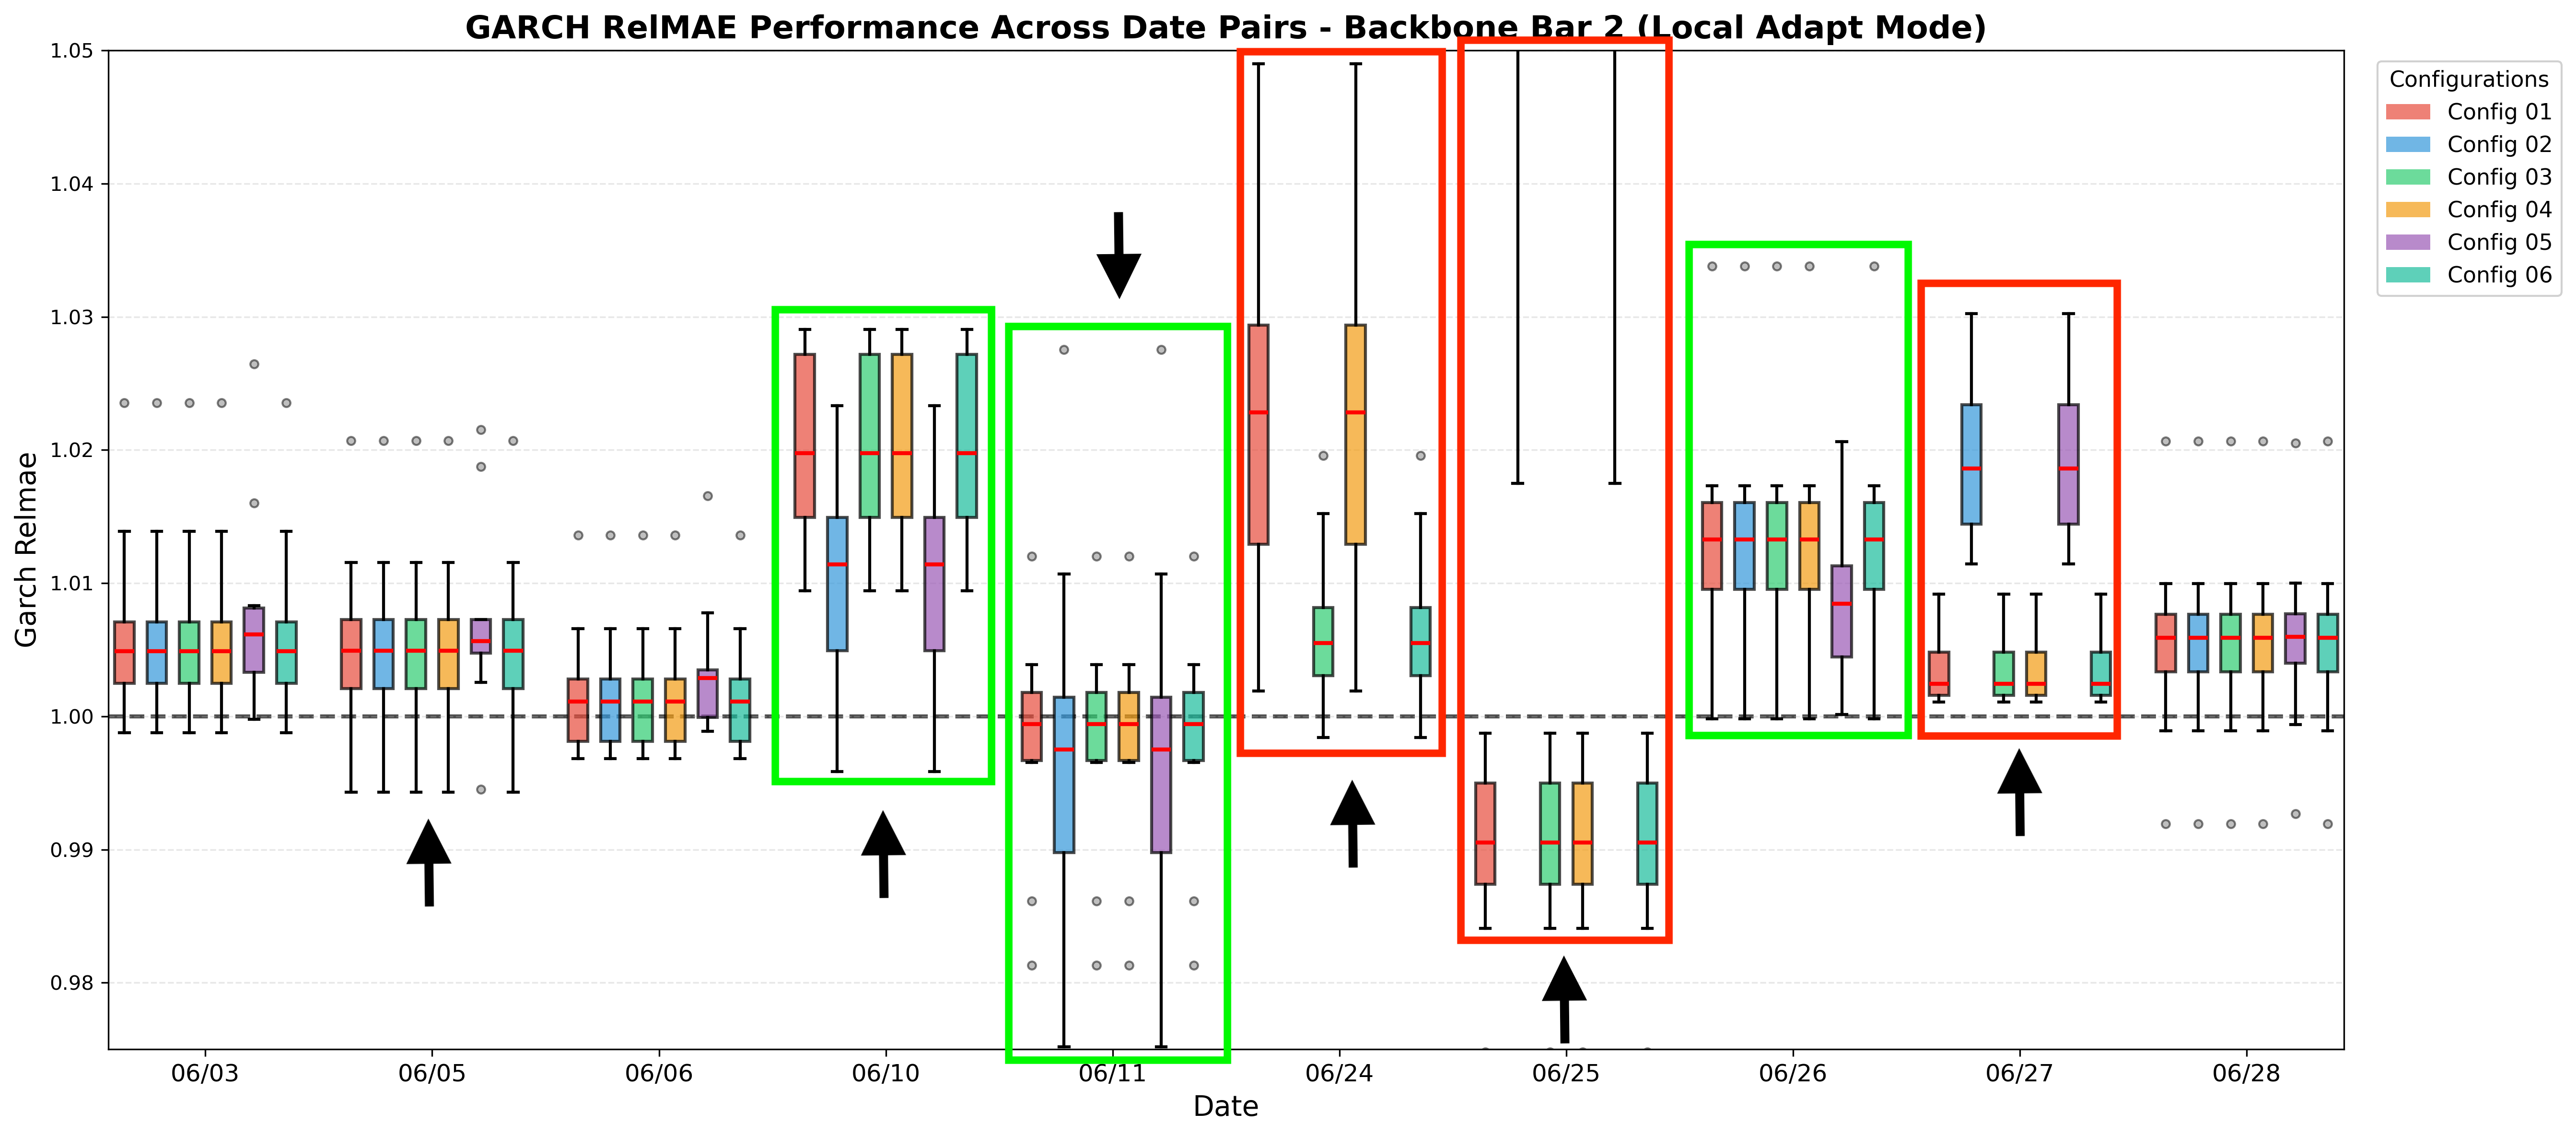
\includegraphics[width=0.9\linewidth]{sequential_boxplot_bb_001_marked.png}
\vspace{0.5em}
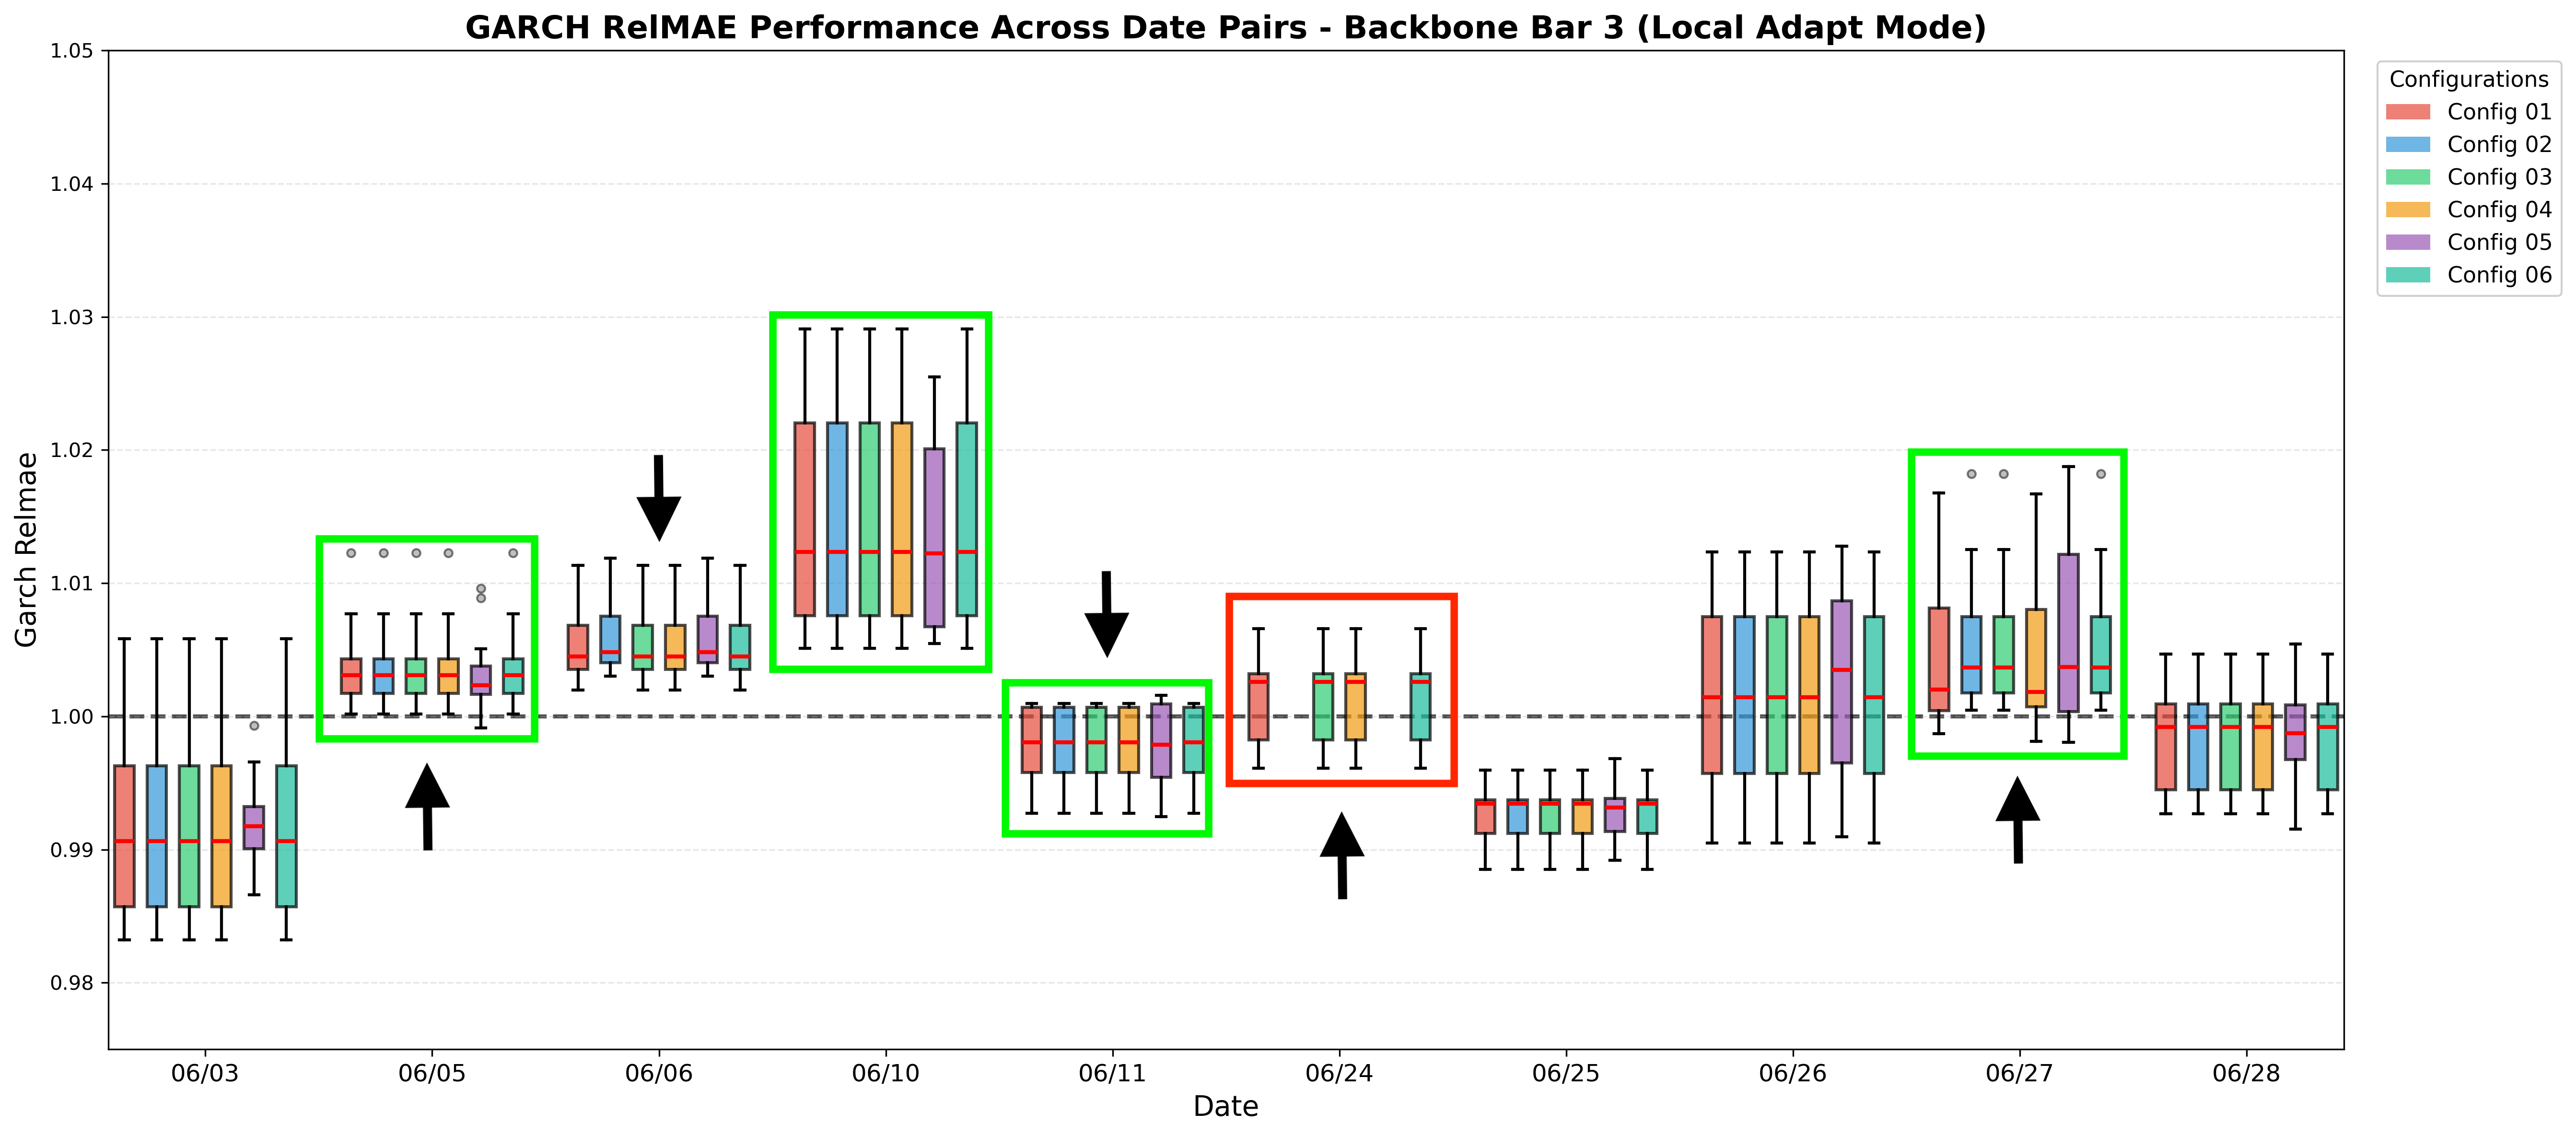
\includegraphics[width=0.9\linewidth]{sequential_boxplot_bb_002_marked.png}

\caption{Sequential RelMAE boxplots for the INTC dataset across date pairs in Local Adapt mode for Backbone Bar 1 (top), Backbone Bar 2 (middle), and Backbone Bar 3 (bottom). The horizontal dashed line at 1.00 represents the naive model baseline. Green rectangles highlight instances where covariate configurations \texttt{05} (raw CNN-LSTM output) or \texttt{01} (full configuration) outperformed configuration \texttt{06} (no covariates). Red rectangles indicate date pairs where configuration \texttt{05} exhibited significant underperformance. Black arrows mark backbone bars where the CNN-LSTM weights were updated during the preceding Global Retrain step. Note that the boxplots corresponding to configurations \texttt{02} and \texttt{05} of Backbone Bars 2 and 3 on 06/24, and Backbone Bar 2 on 06/27, lie above the superior margin.}
\label{fig:sequential_boxplot_intc_data}
\end{figure}

$r^w_j$ $\mathrm{CNNLSTM}_{\mathbf{W}}\!\left(\widetilde{\mathbf{OF}}^{\mathcal{P}^{(E)}}_{i_{t-1}-99:i_{t-1}}\right)$ $OFI_{0, j}$

\begin{figure}[ht!]
\centering
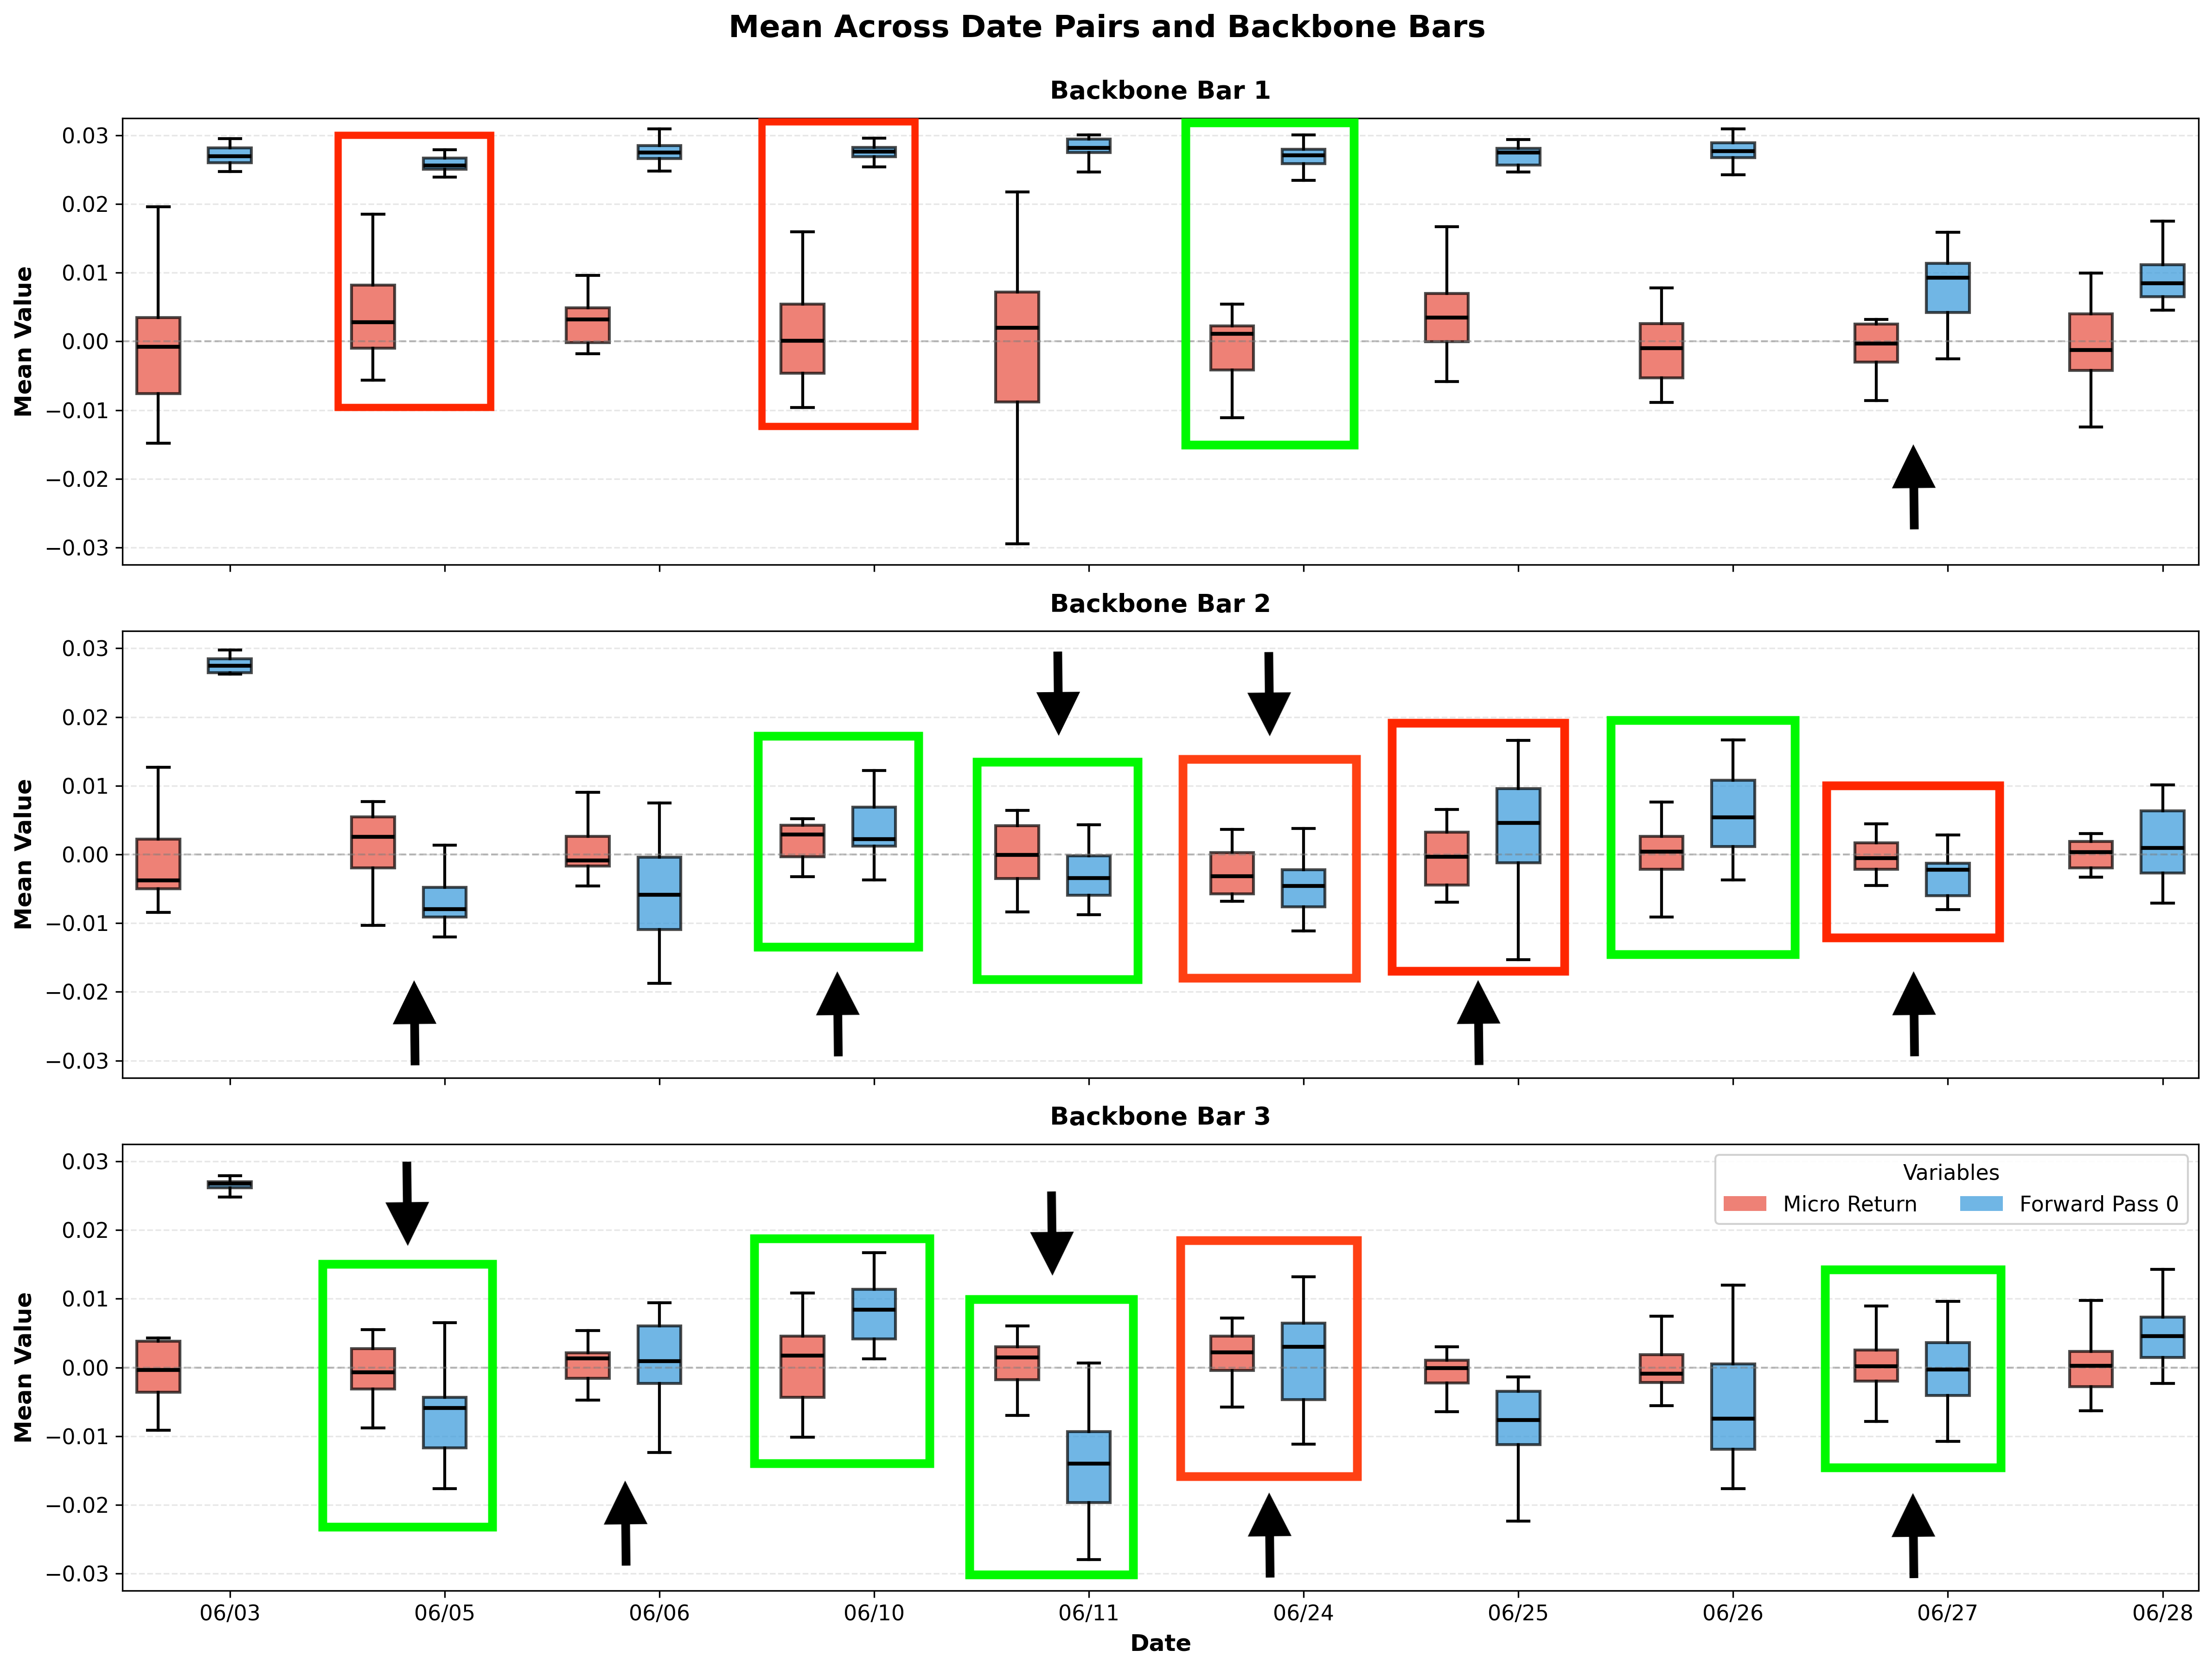
\includegraphics[width=0.9\linewidth]{covariate_aggregate_mean_boxplots_marked.png}
\caption{Distribution of the \textbf{mean} of the Micro-Return ($r^w_j$) and CNN-LSTM Output ($\mathrm{CNNLSTM}_{\mathbf{W}}\!\left(\widetilde{\mathbf{OF}}^{\mathcal{P}^{(E)}}_{i_{t-1}-99:i_{t-1}}\right)$) computed on each adapter bar and aggregated at the backbone bar level. See Figure~\ref{fig:sequential_boxplot_intc_data} for the interpretation of the markers.}
\label{fig:covariate_aggregate_mean}
\end{figure}

\begin{figure}[ht!]
\centering
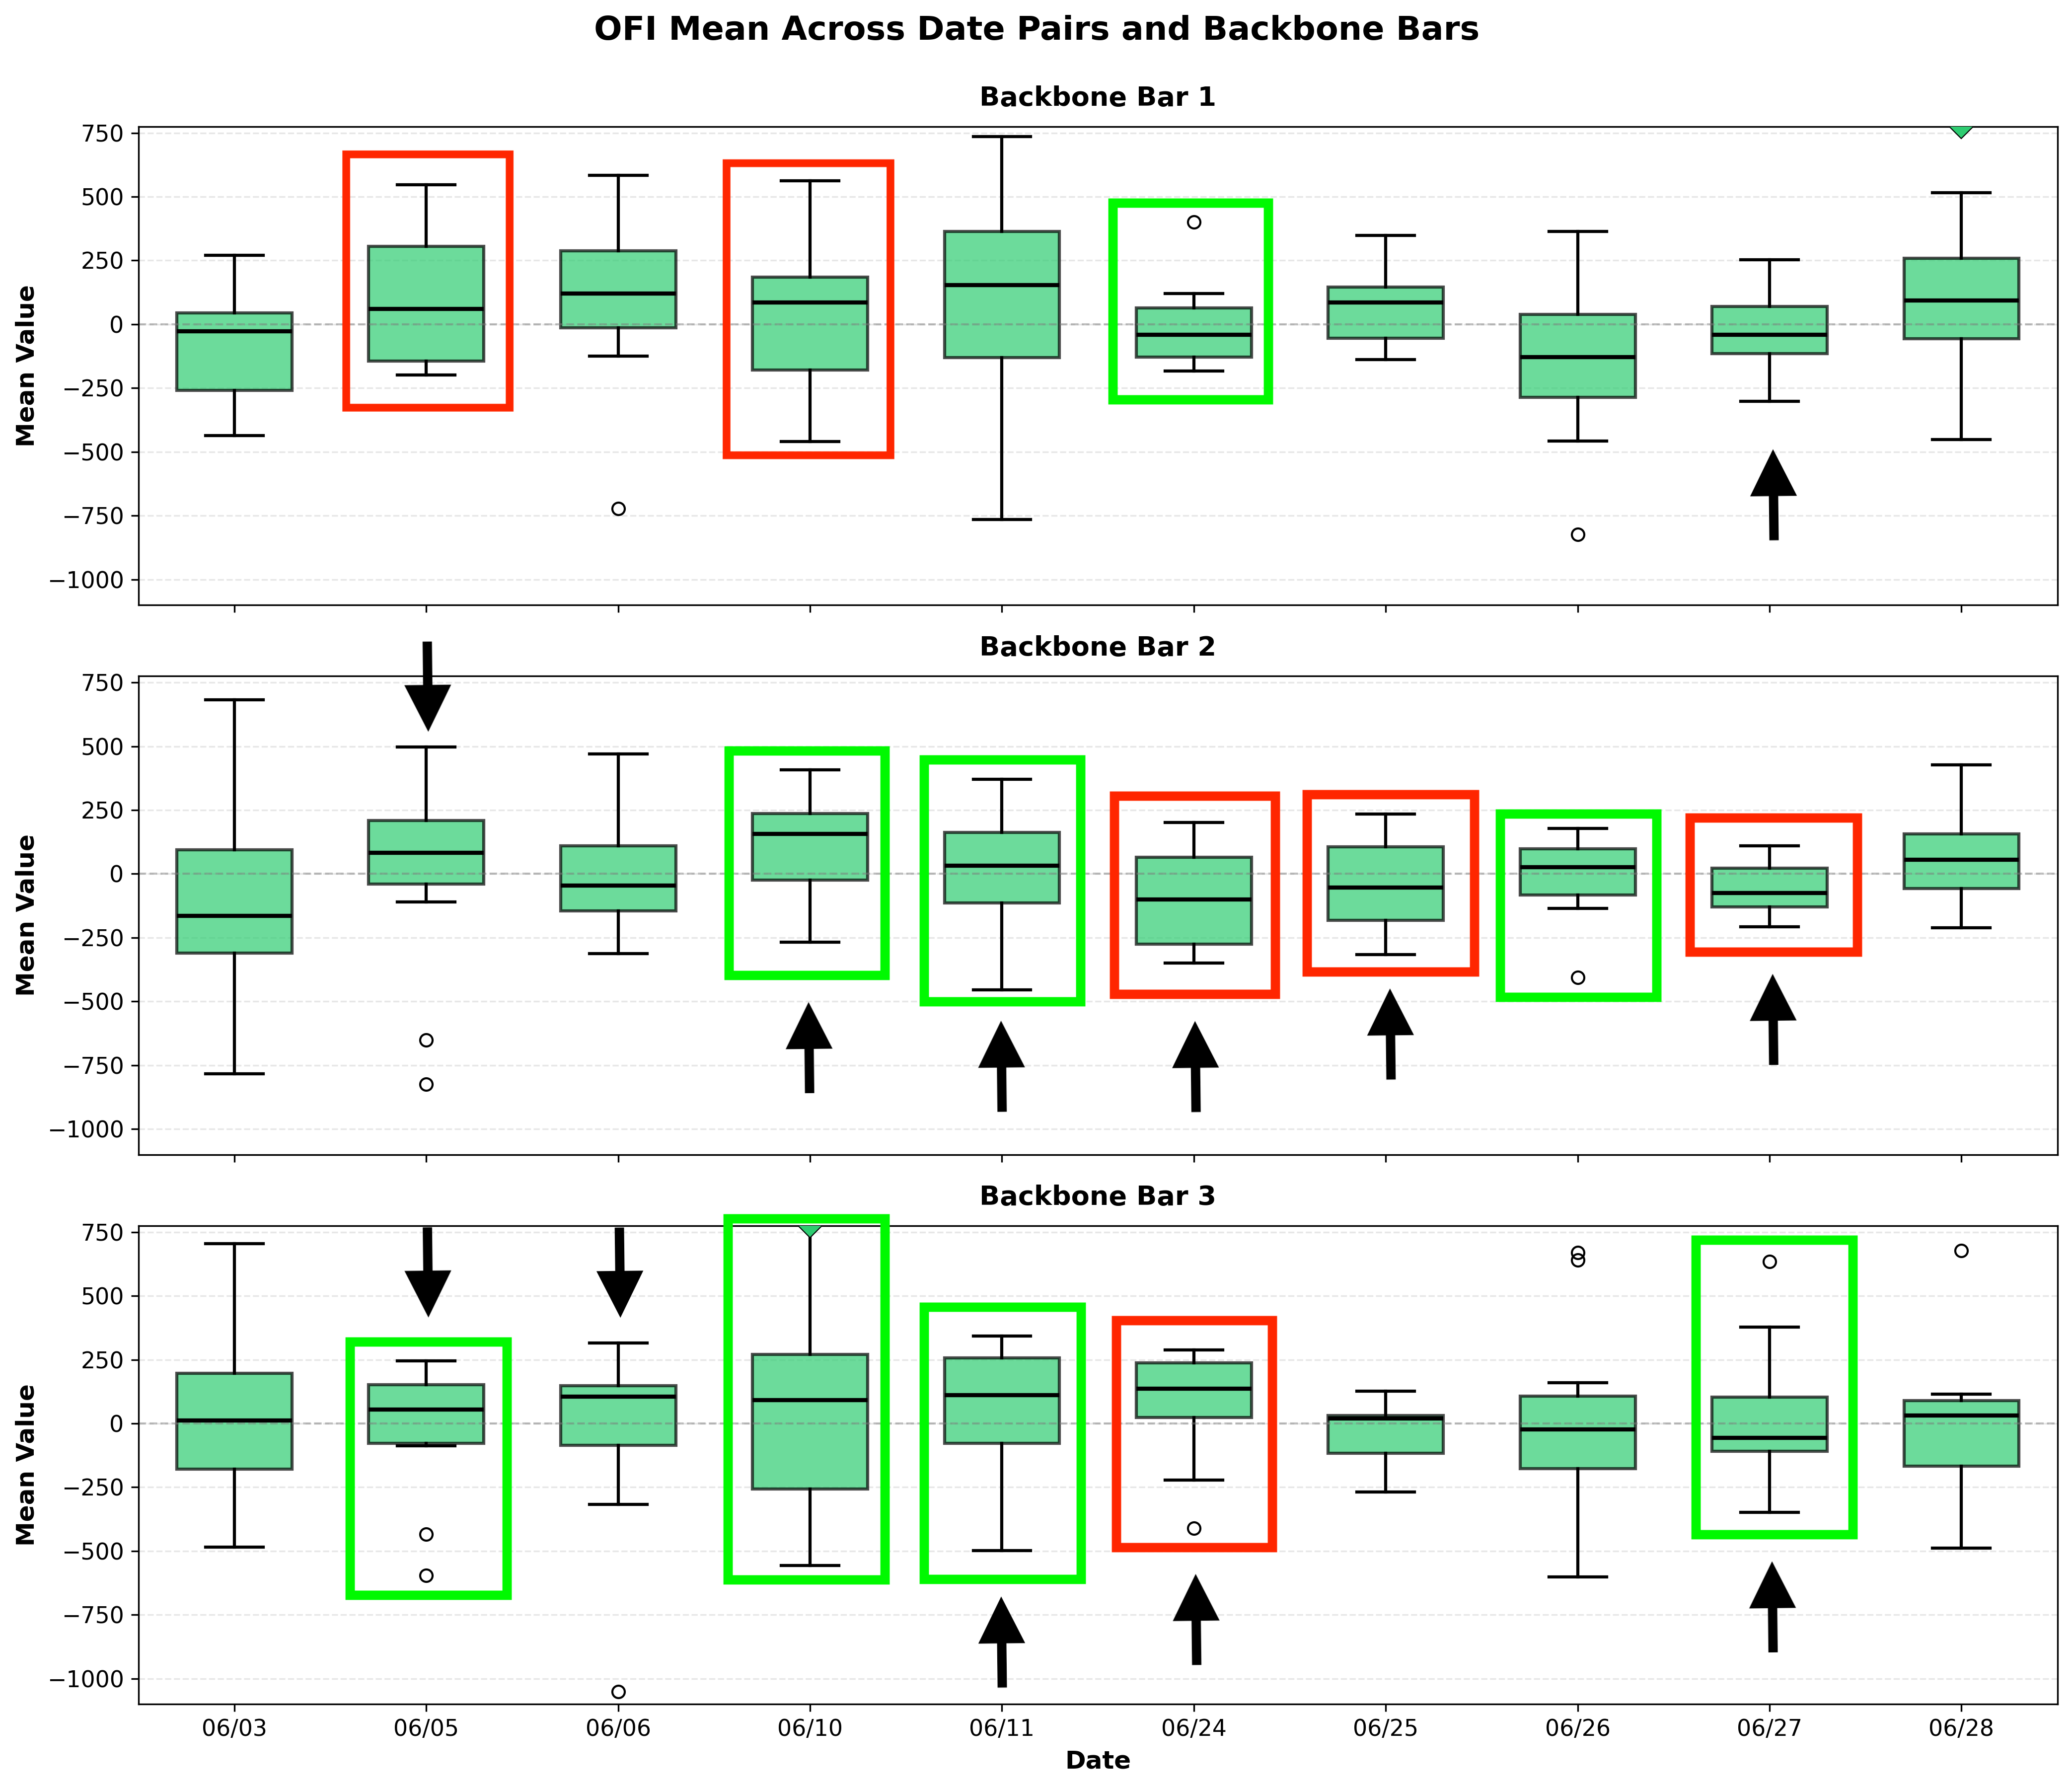
\includegraphics[width=0.9\linewidth]{ofi_aggregate_mean_boxplots_marked.png}
\caption{Distribution of the \textbf{mean} of the Order Flow Imbalance at touch ($OFI_{0, j}$) computed on each adapter bar and aggregated at the backbone bar level. See Figure~\ref{fig:sequential_boxplot_intc_data} for the interpretation of the markers.}
\label{fig:ofi_aggregate_mean}
\end{figure}

\begin{figure}[ht!]
\centering
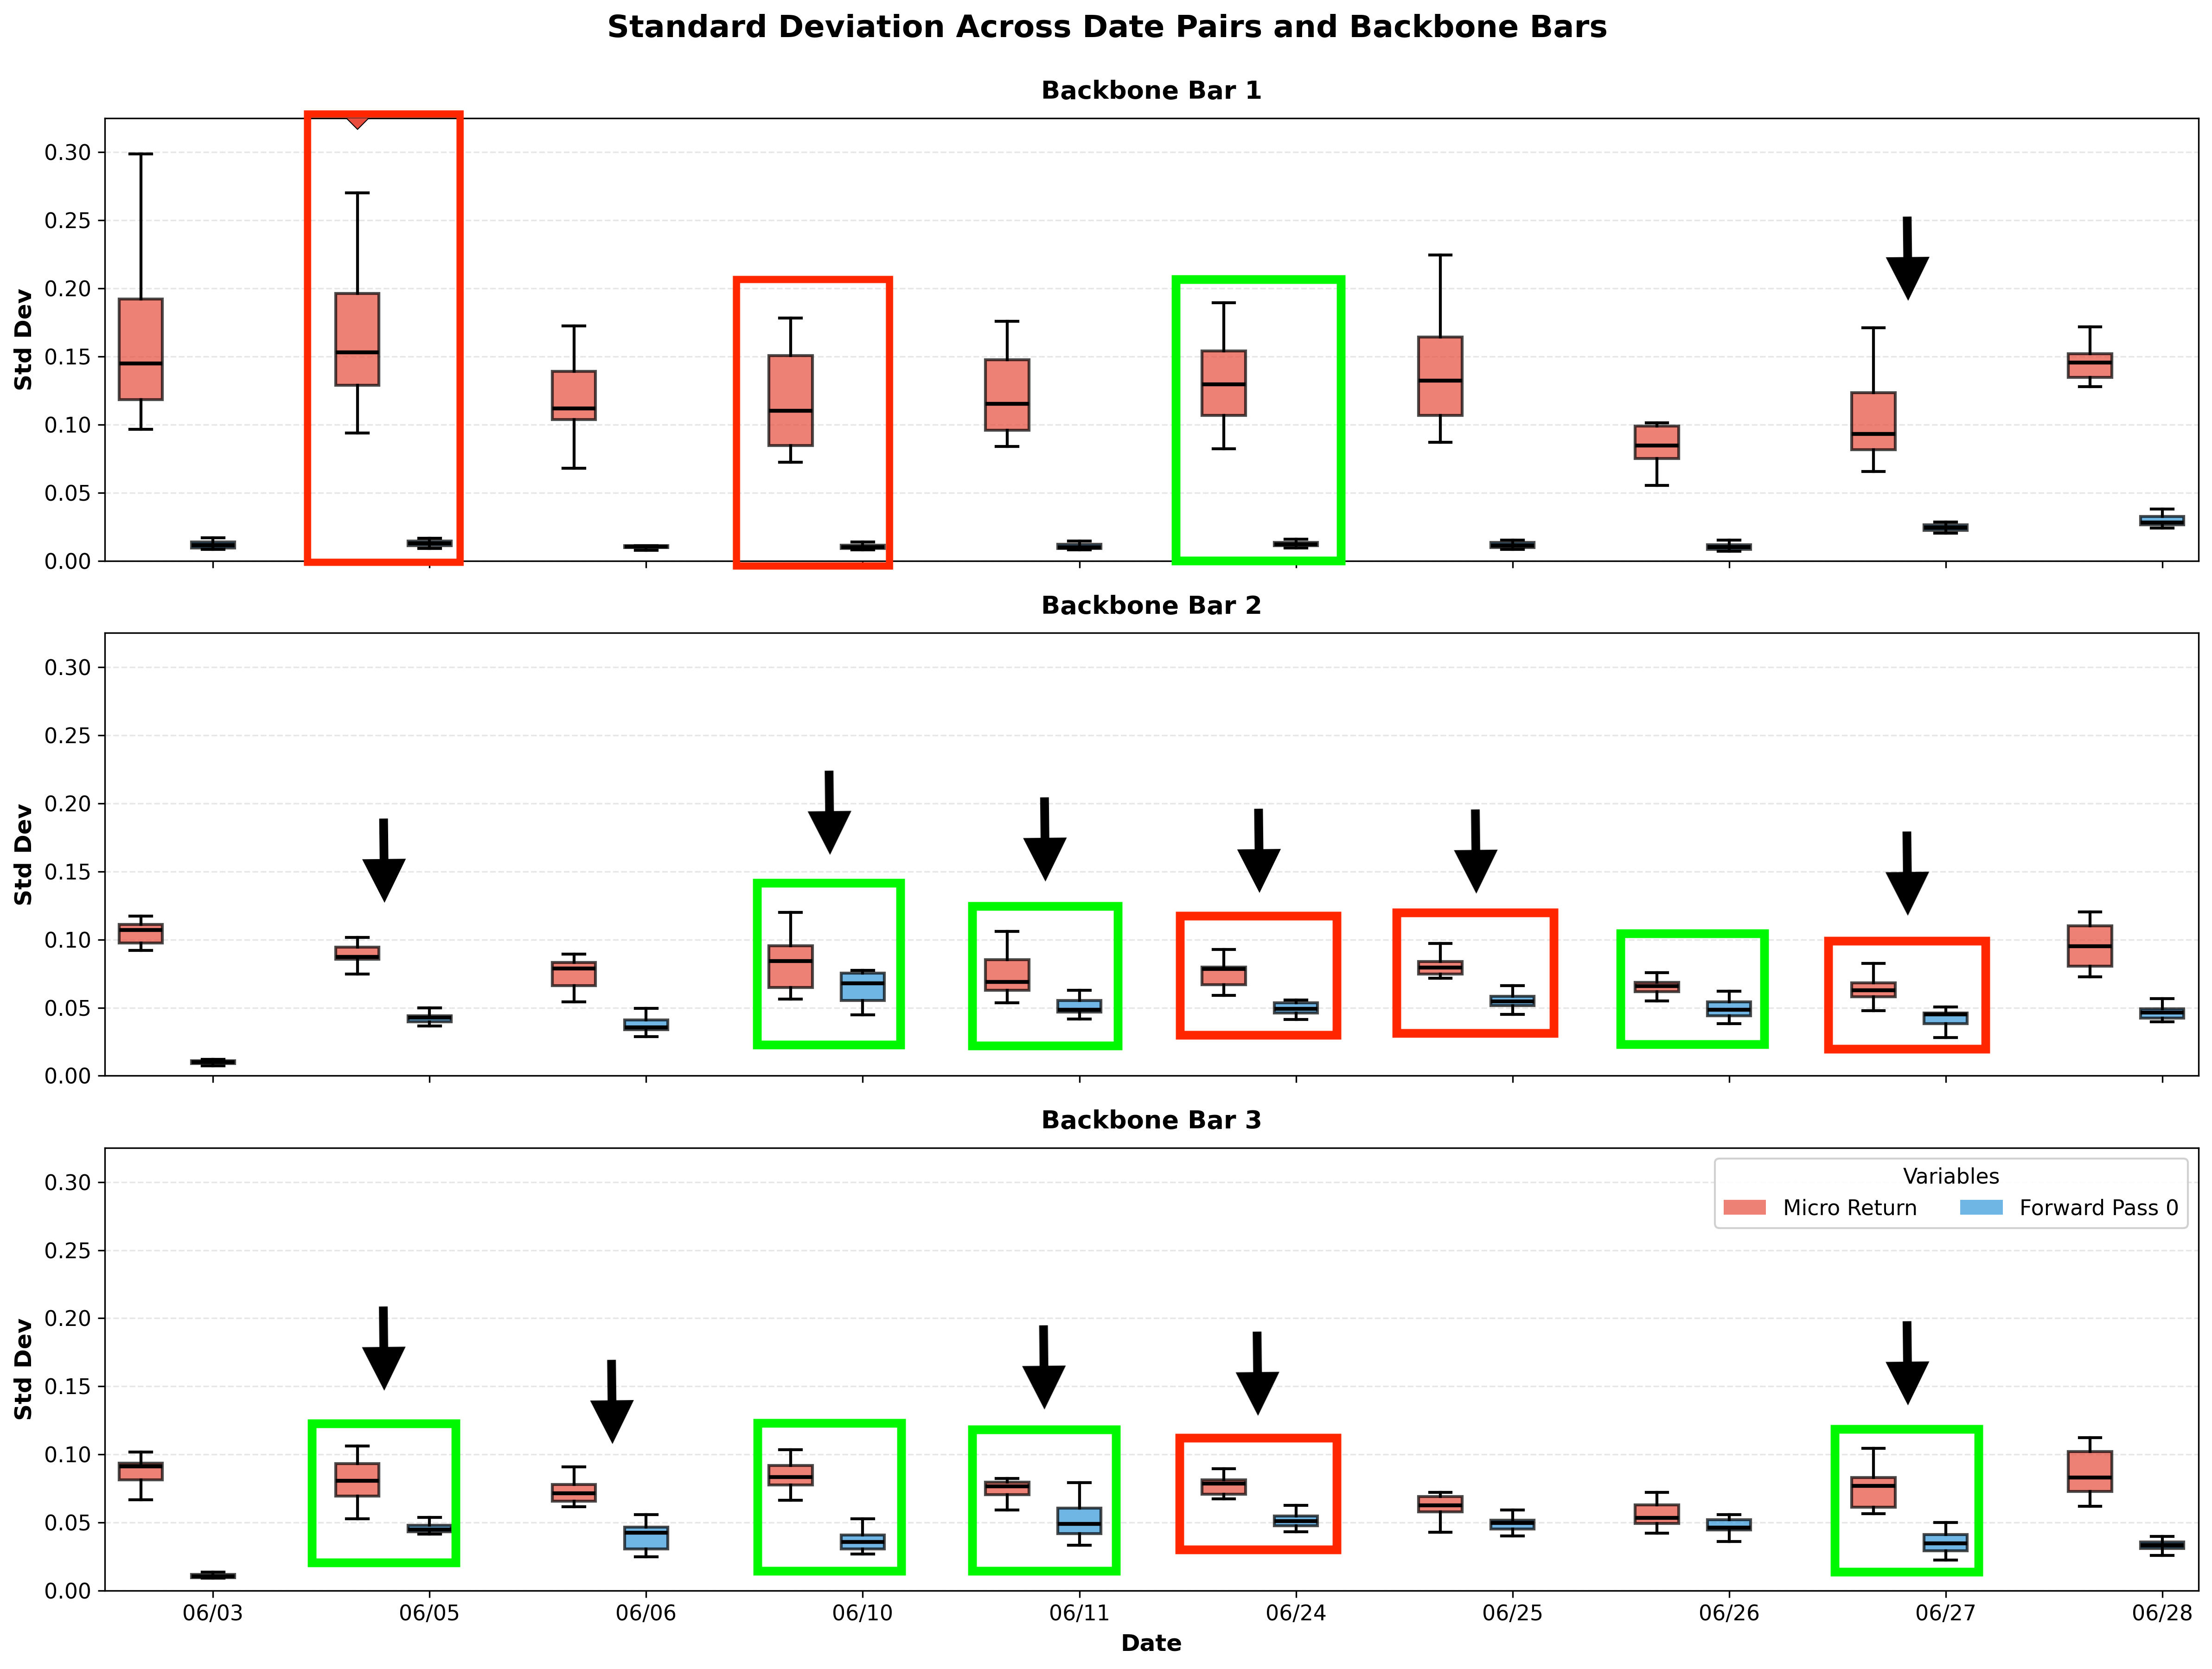
\includegraphics[width=0.9\linewidth]{covariate_aggregate_std_boxplots_marked.png}
\caption{Distribution of the \textbf{standard deviation} of the Micro-Return ($r^w_j$) and CNN-LSTM Output ($\mathrm{CNNLSTM}_{\mathbf{W}}\!\left(\widetilde{\mathbf{OF}}^{\mathcal{P}^{(E)}}_{i_{t-1}-99:i_{t-1}}\right)$) computed on each adapter bar and aggregated at the backbone bar level. See Figure~\ref{fig:sequential_boxplot_intc_data} for the interpretation of the markers.}
\label{fig:covariate_aggregate_std}
\end{figure}

\begin{figure}[ht!]
\centering
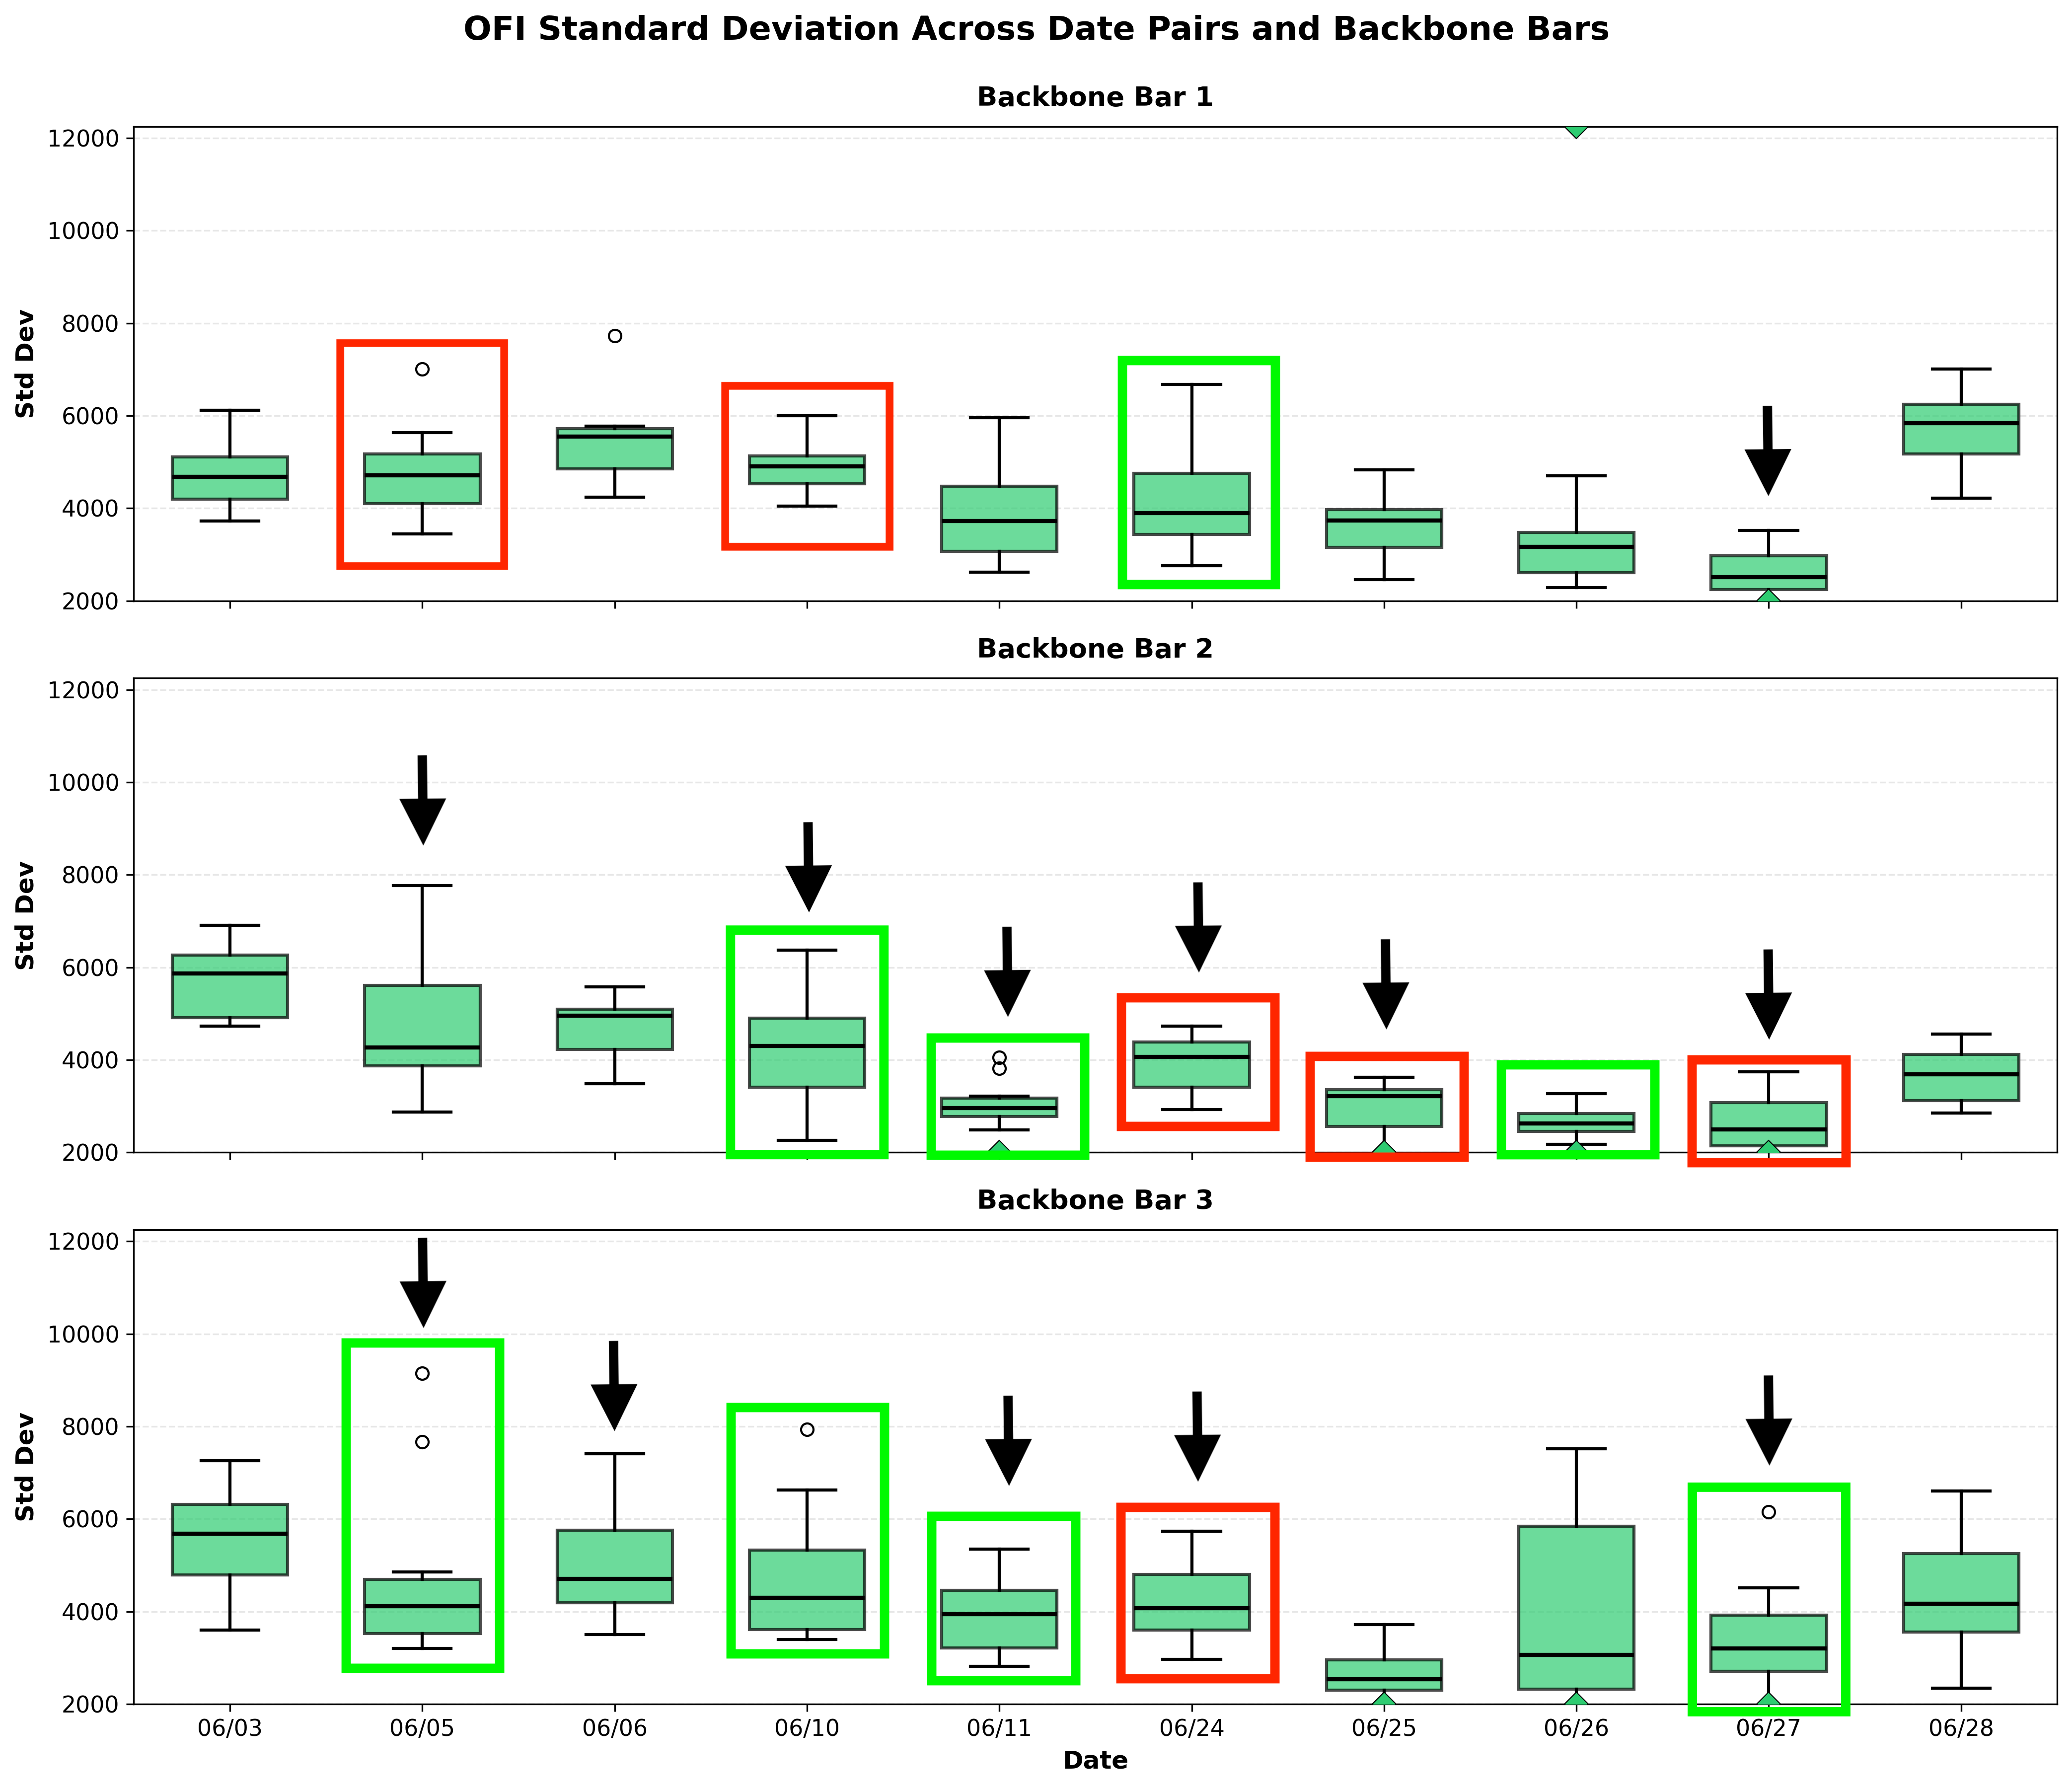
\includegraphics[width=0.9\linewidth]{ofi_aggregate_std_boxplots_marked.png}
\caption{Distribution of the \textbf{standard deviation} of the Order Flow Imbalance at touch ($OFI_{0, j}$) computed on each adapter bar and aggregated at the backbone bar level. See Figure~\ref{fig:sequential_boxplot_intc_data} for the interpretation of the markers.}
\label{fig:ofi_aggregate_std}
\end{figure}


\begin{figure}[ht!]
\centering
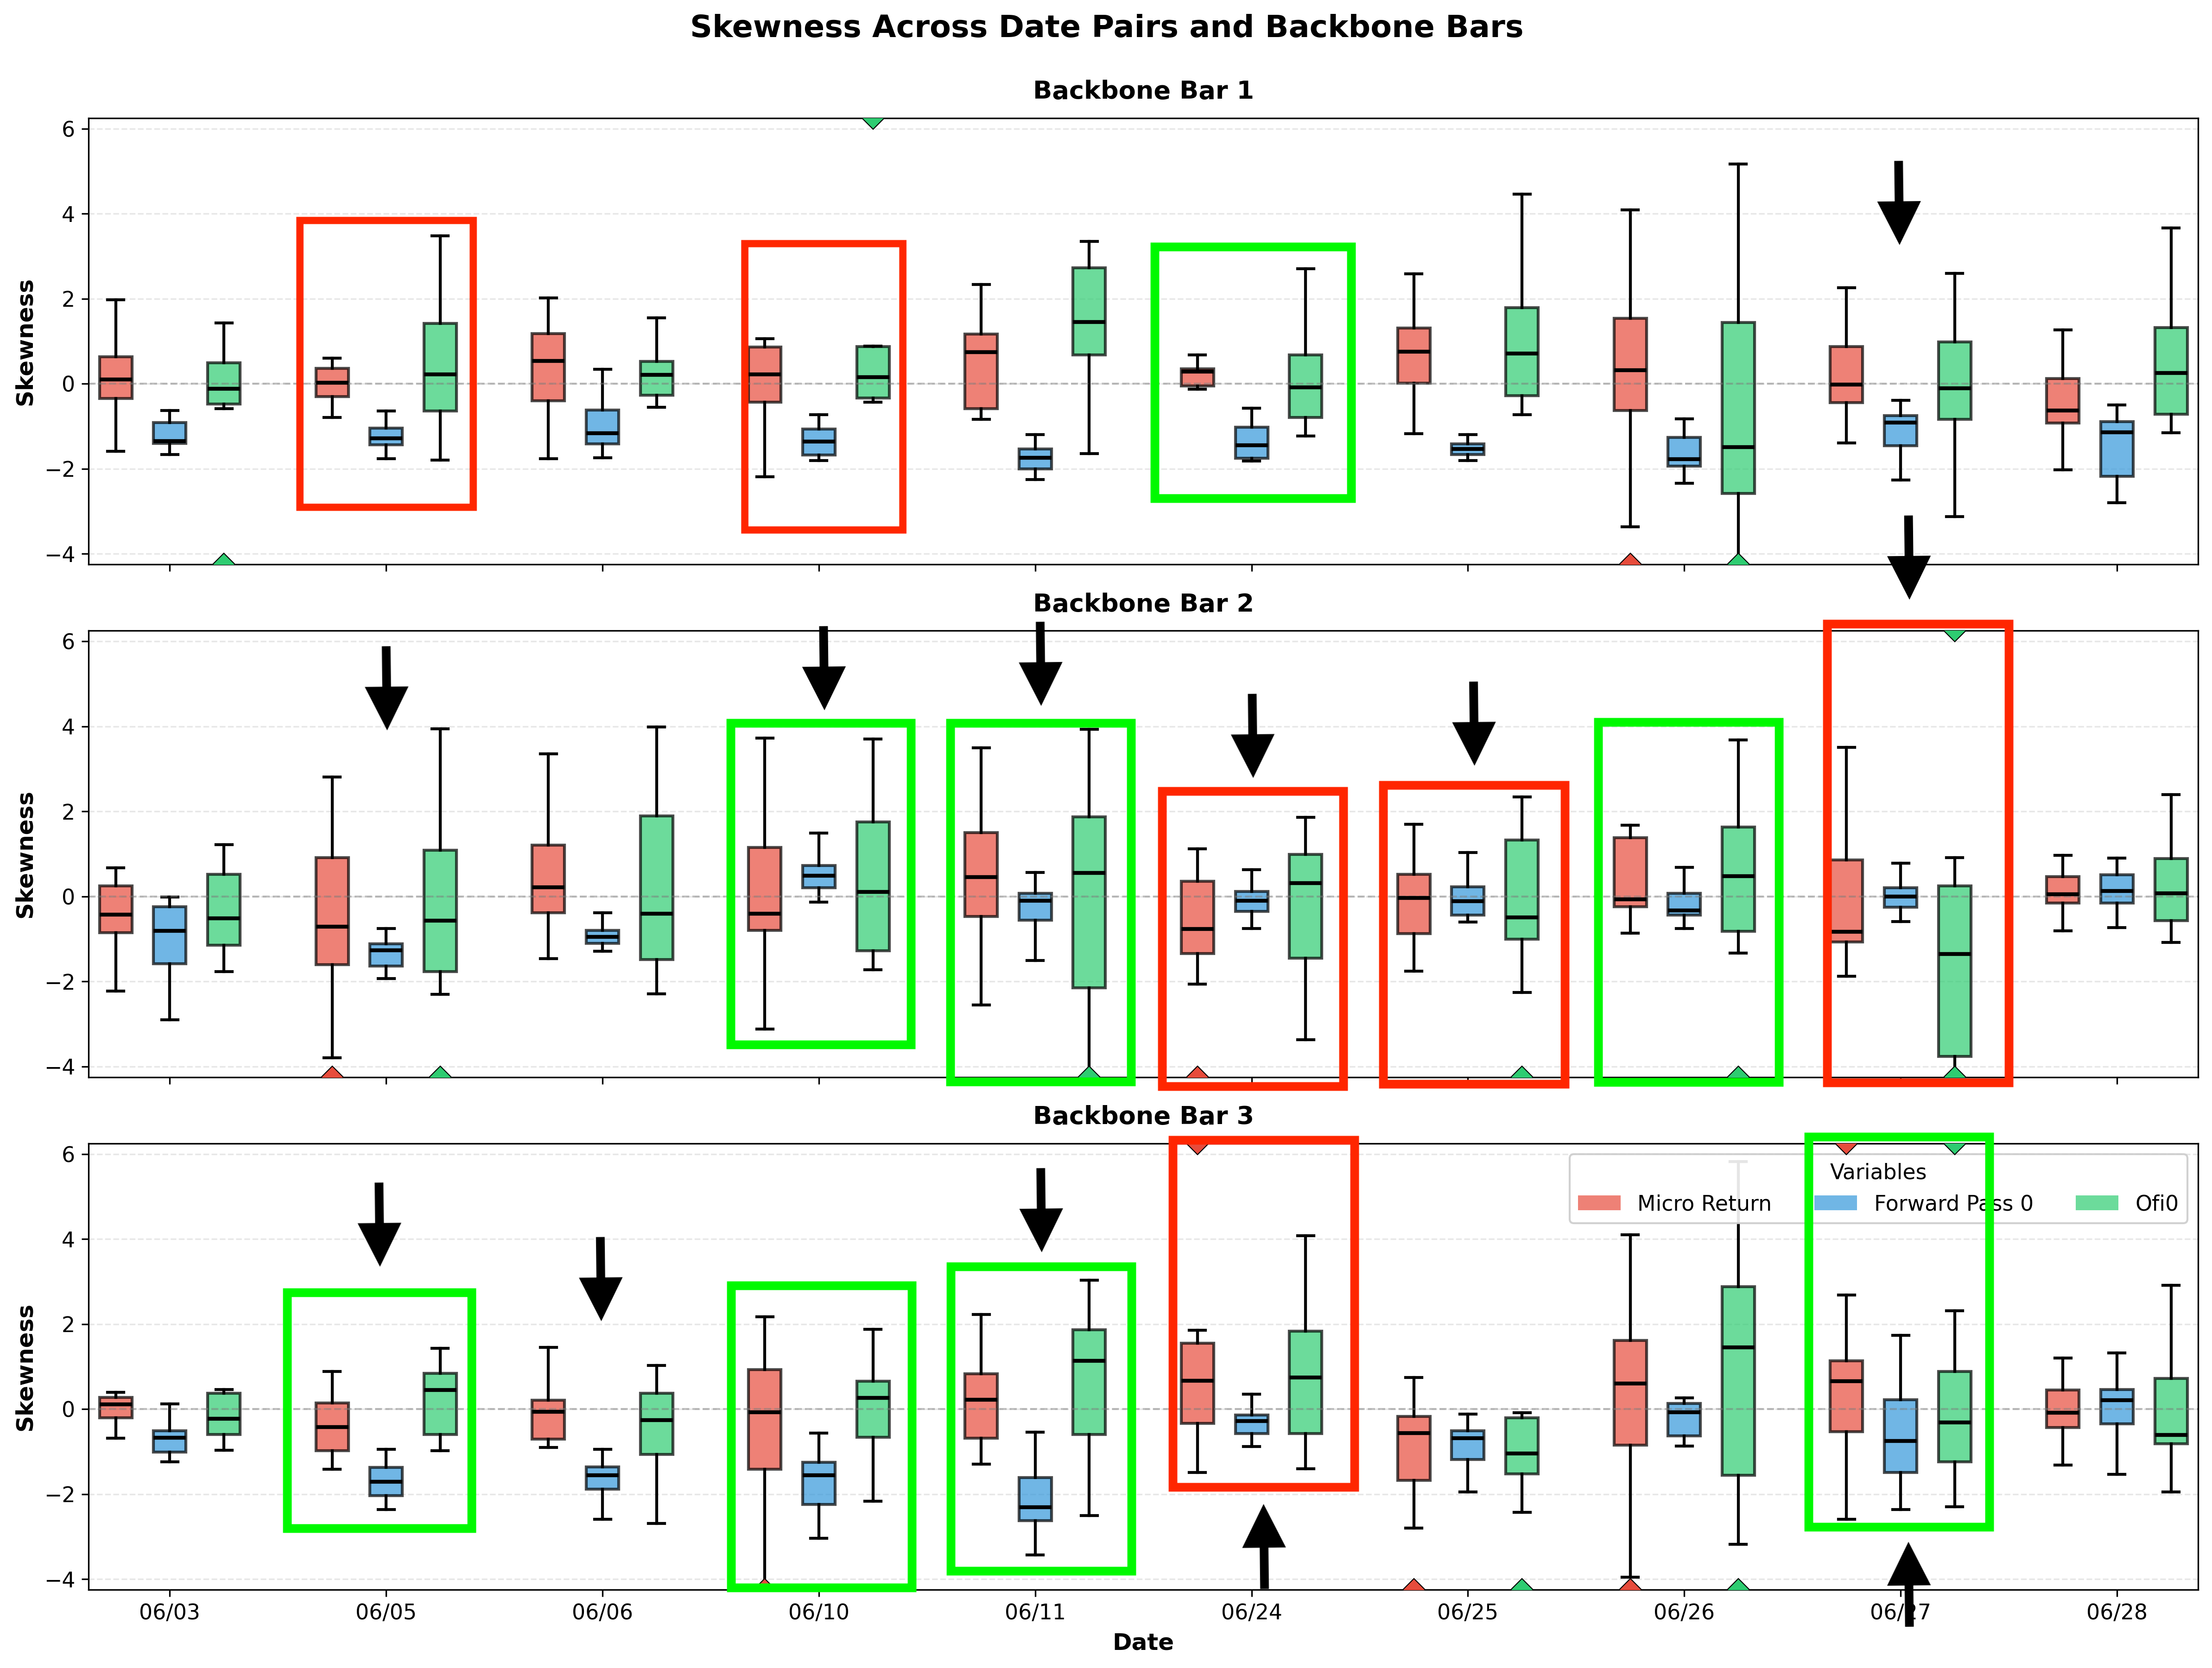
\includegraphics[width=0.9\linewidth]{covariate_aggregate_skewness_boxplots_marked.png}
\caption{Distribution of the \textbf{skewness} of the Micro-Return ($r^w_j$), CNN-LSTM Output ($\mathrm{CNNLSTM}_{\mathbf{W}}\!\left(\widetilde{\mathbf{OF}}^{\mathcal{P}^{(E)}}_{i_{t-1}-99:i_{t-1}}\right)$), and Order Flow Imbalance at touch ($OFI_{0, j}$) computed on each adapter bar and aggregated at the backbone bar level. See Figure~\ref{fig:sequential_boxplot_intc_data} for the interpretation of the markers.}
\label{fig:covariate_aggregate_skewness}
\end{figure}

\begin{figure}[ht!]
\centering
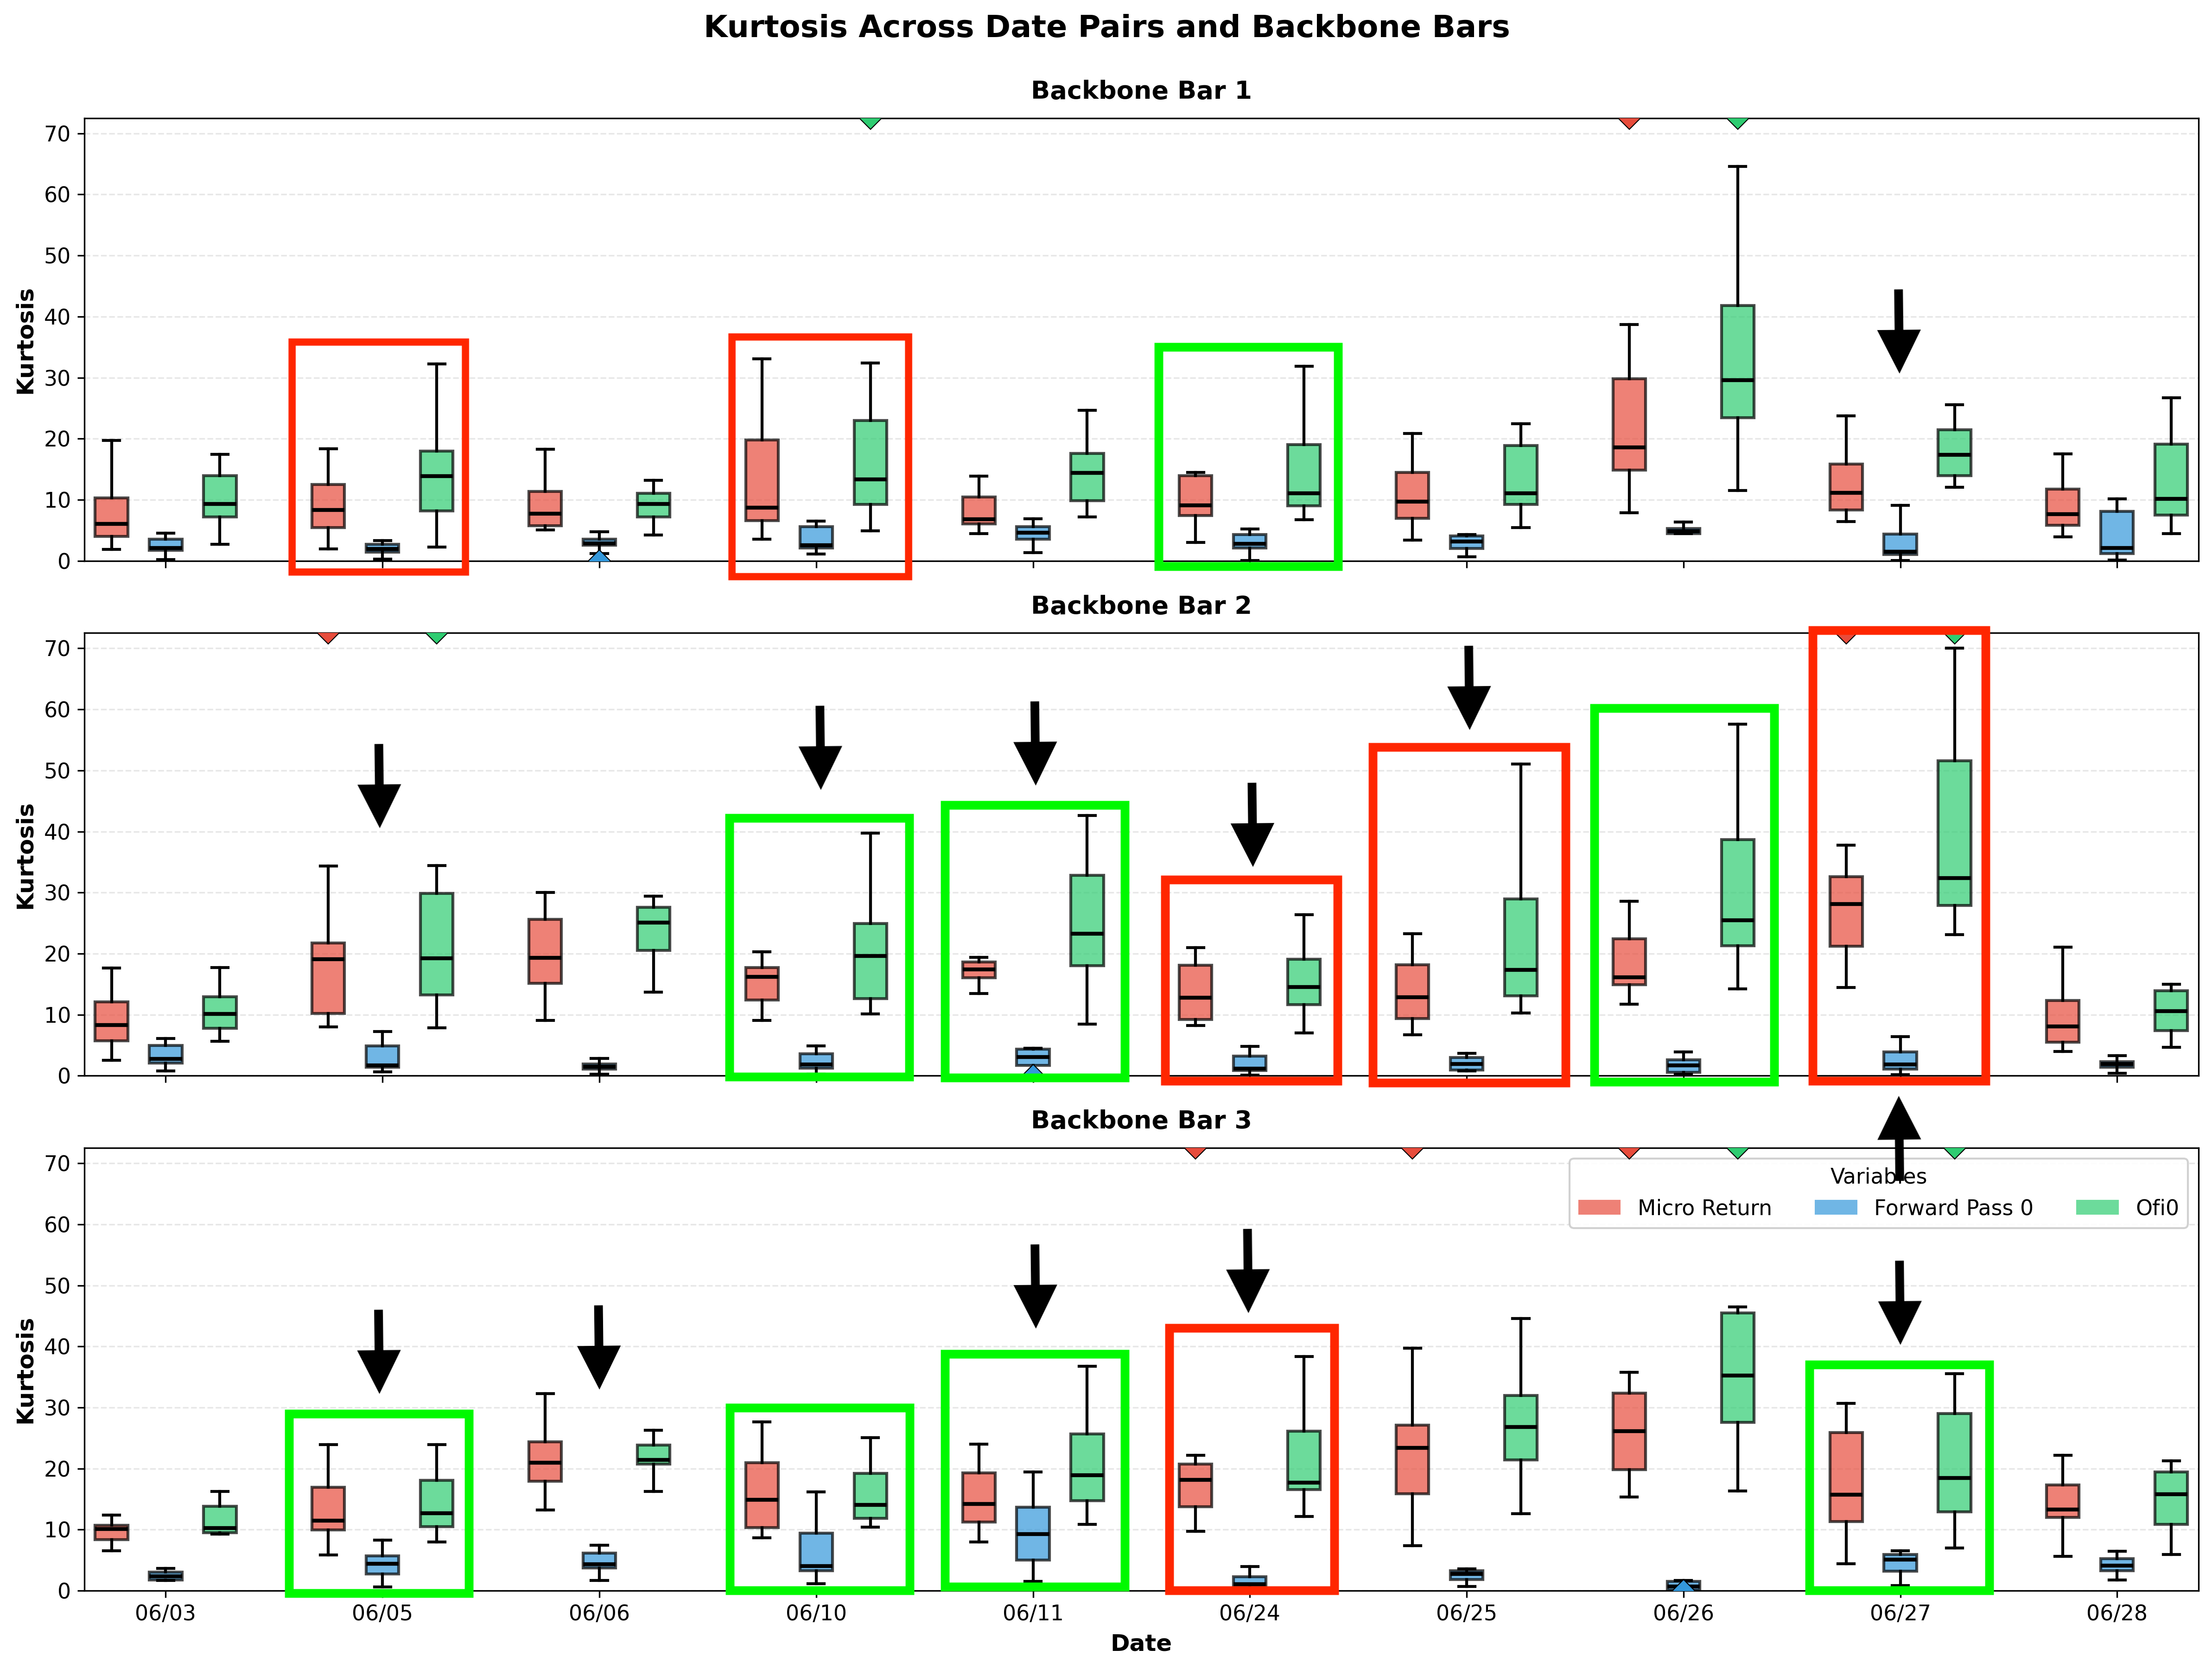
\includegraphics[width=0.9\linewidth]{covariate_aggregate_kurtosis_boxplots_marked.png}
\caption{Distribution of the \textbf{kurtosis} of the Micro-Return ($r^w_j$), CNN-LSTM Output ($\mathrm{CNNLSTM}_{\mathbf{W}}\!\left(\widetilde{\mathbf{OF}}^{\mathcal{P}^{(E)}}_{i_{t-1}-99:i_{t-1}}\right)$), and Order Flow Imbalance at touch ($OFI_{0, j}$) computed on each adapter bar and aggregated at the backbone bar level. See Figure~\ref{fig:sequential_boxplot_intc_data} for the interpretation of the markers.}
\label{fig:covariate_aggregate_kurtosis}
\end{figure}

\begin{figure}[ht!]
\centering
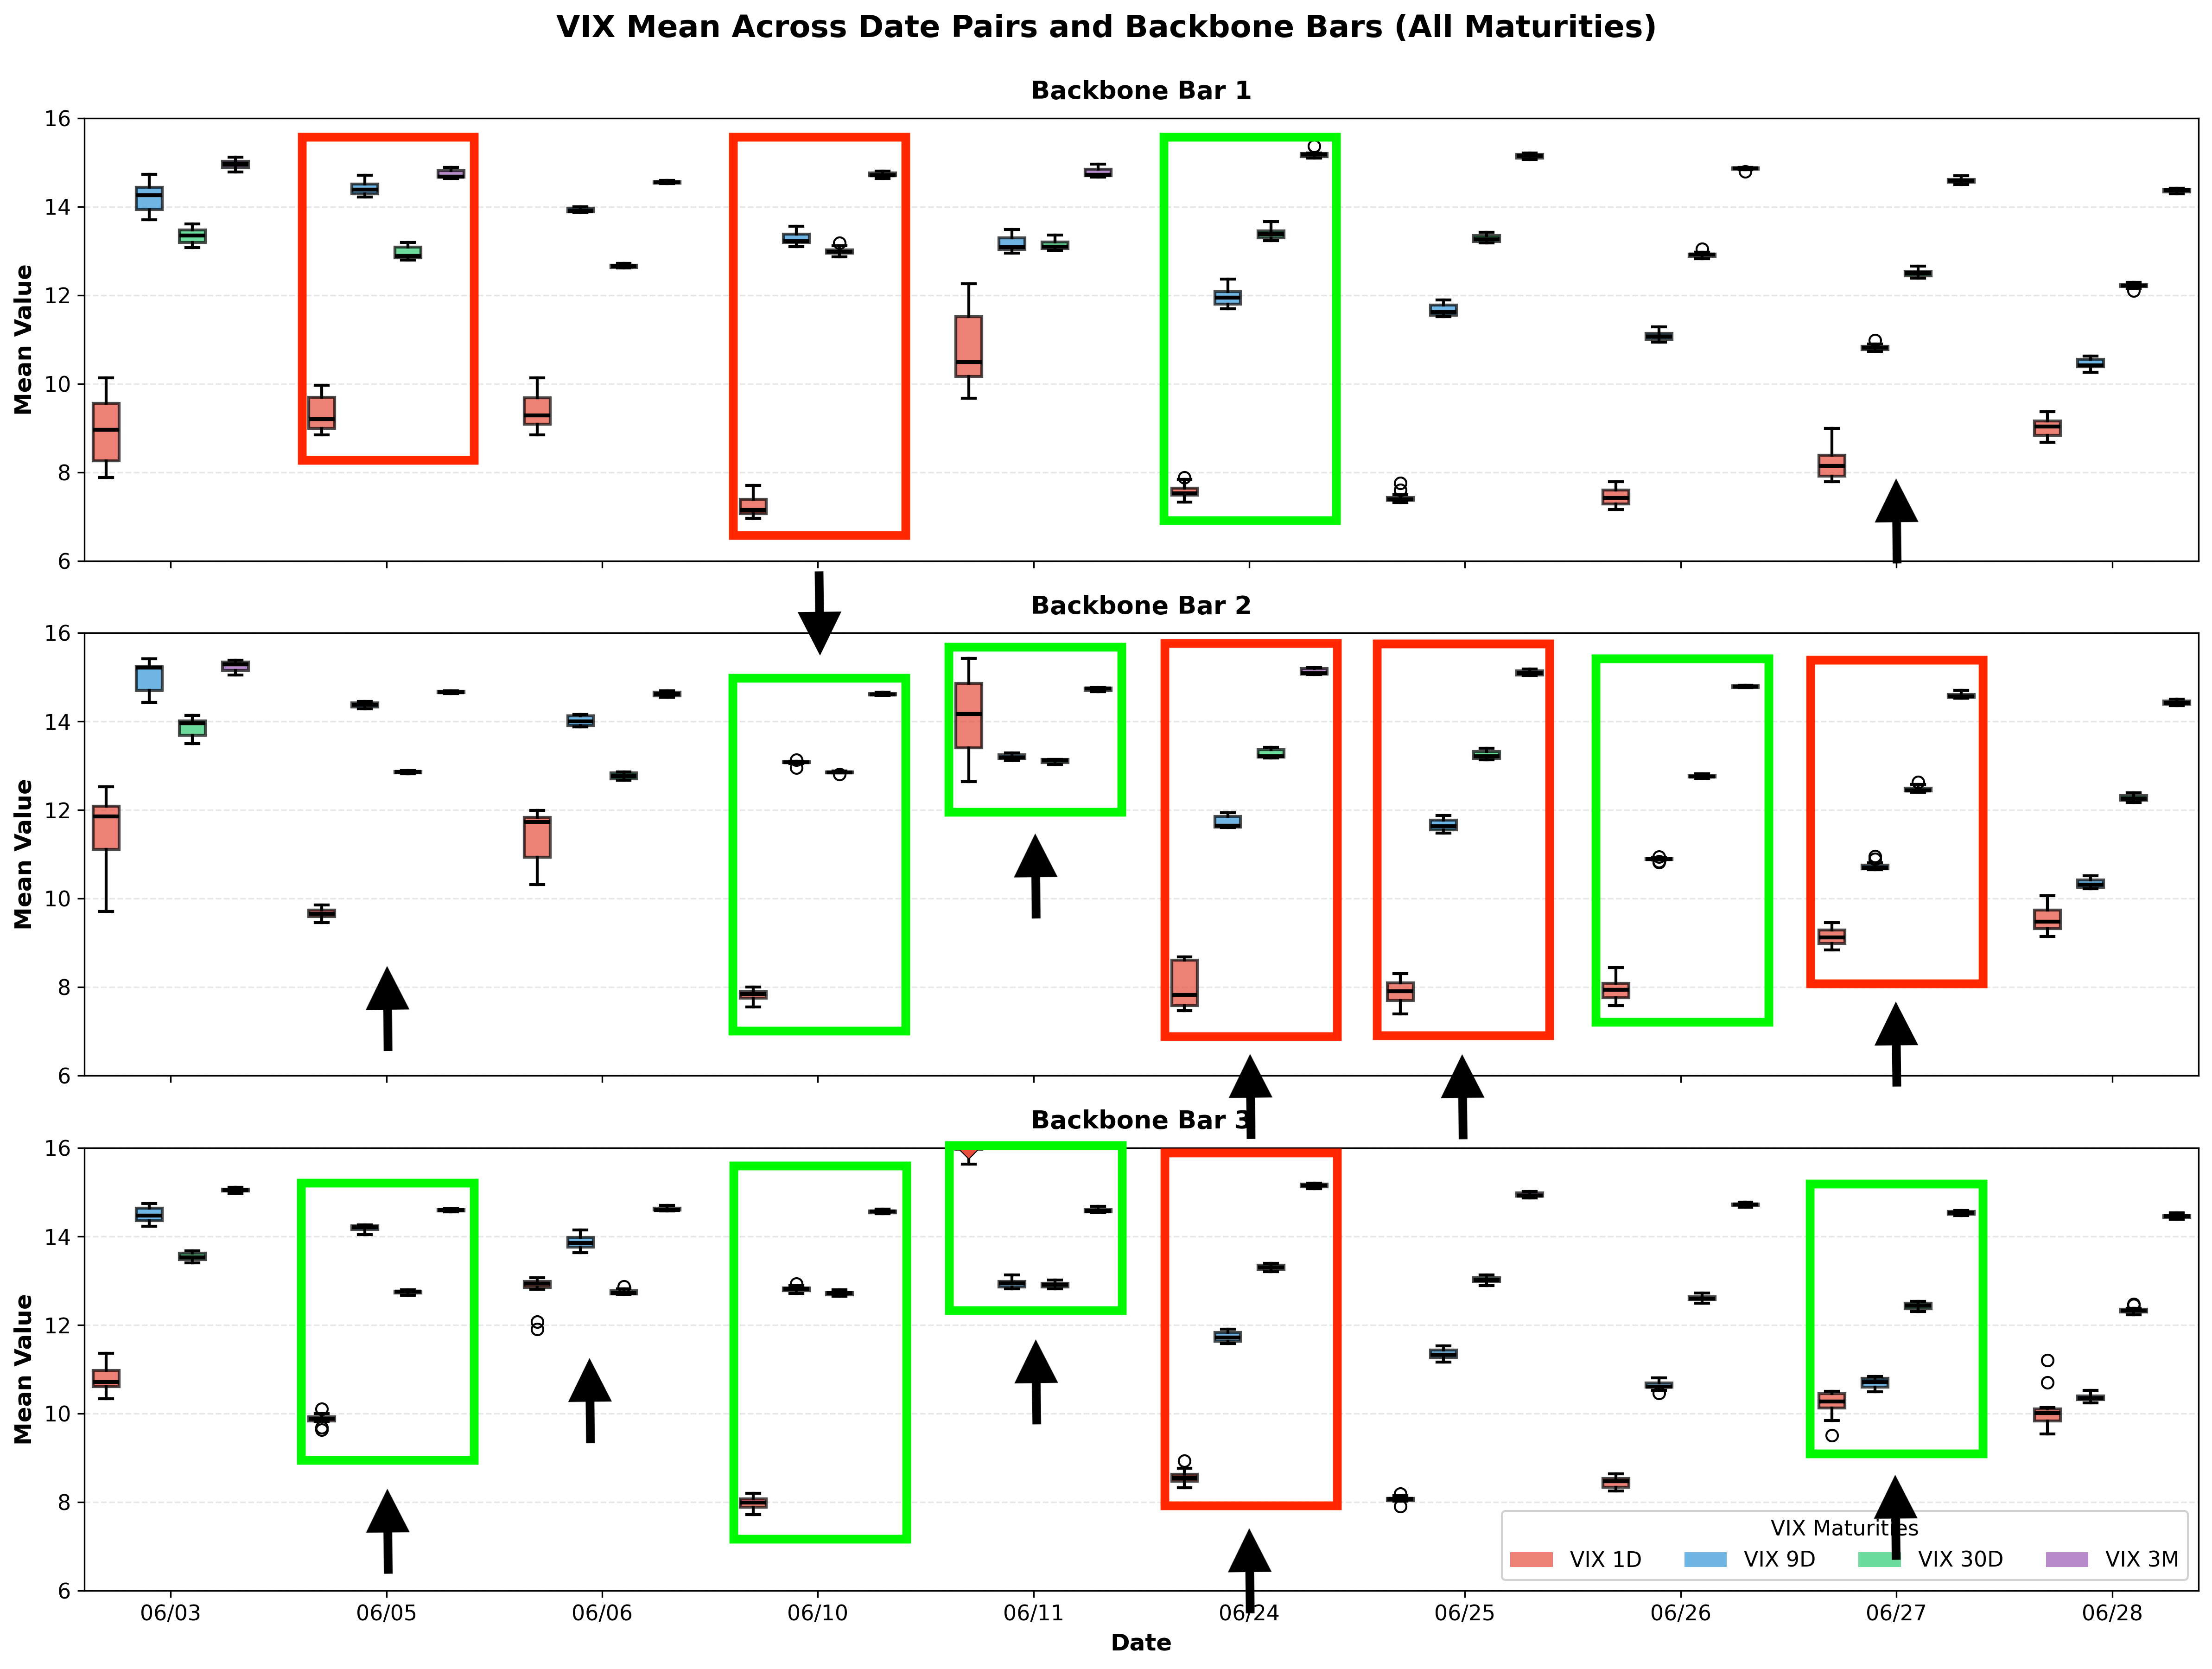
\includegraphics[width=0.9\linewidth]{vix_aggregate_mean_boxplots_marked.png}
\caption{Distribution of the \textbf{mean} of the VIX indices ($VIX_t^{(\tau)}$ for $\tau \in \{ \text{1d}, \text{9d}, \text{30d}, \text{3m} \}$) computed on each adapter bar and aggregated at the backbone bar level. See Figure~\ref{fig:sequential_boxplot_intc_data} for the interpretation of the markers.}
\label{fig:vix_aggregate_mean}
\end{figure}

\begin{figure}[ht!]
\centering
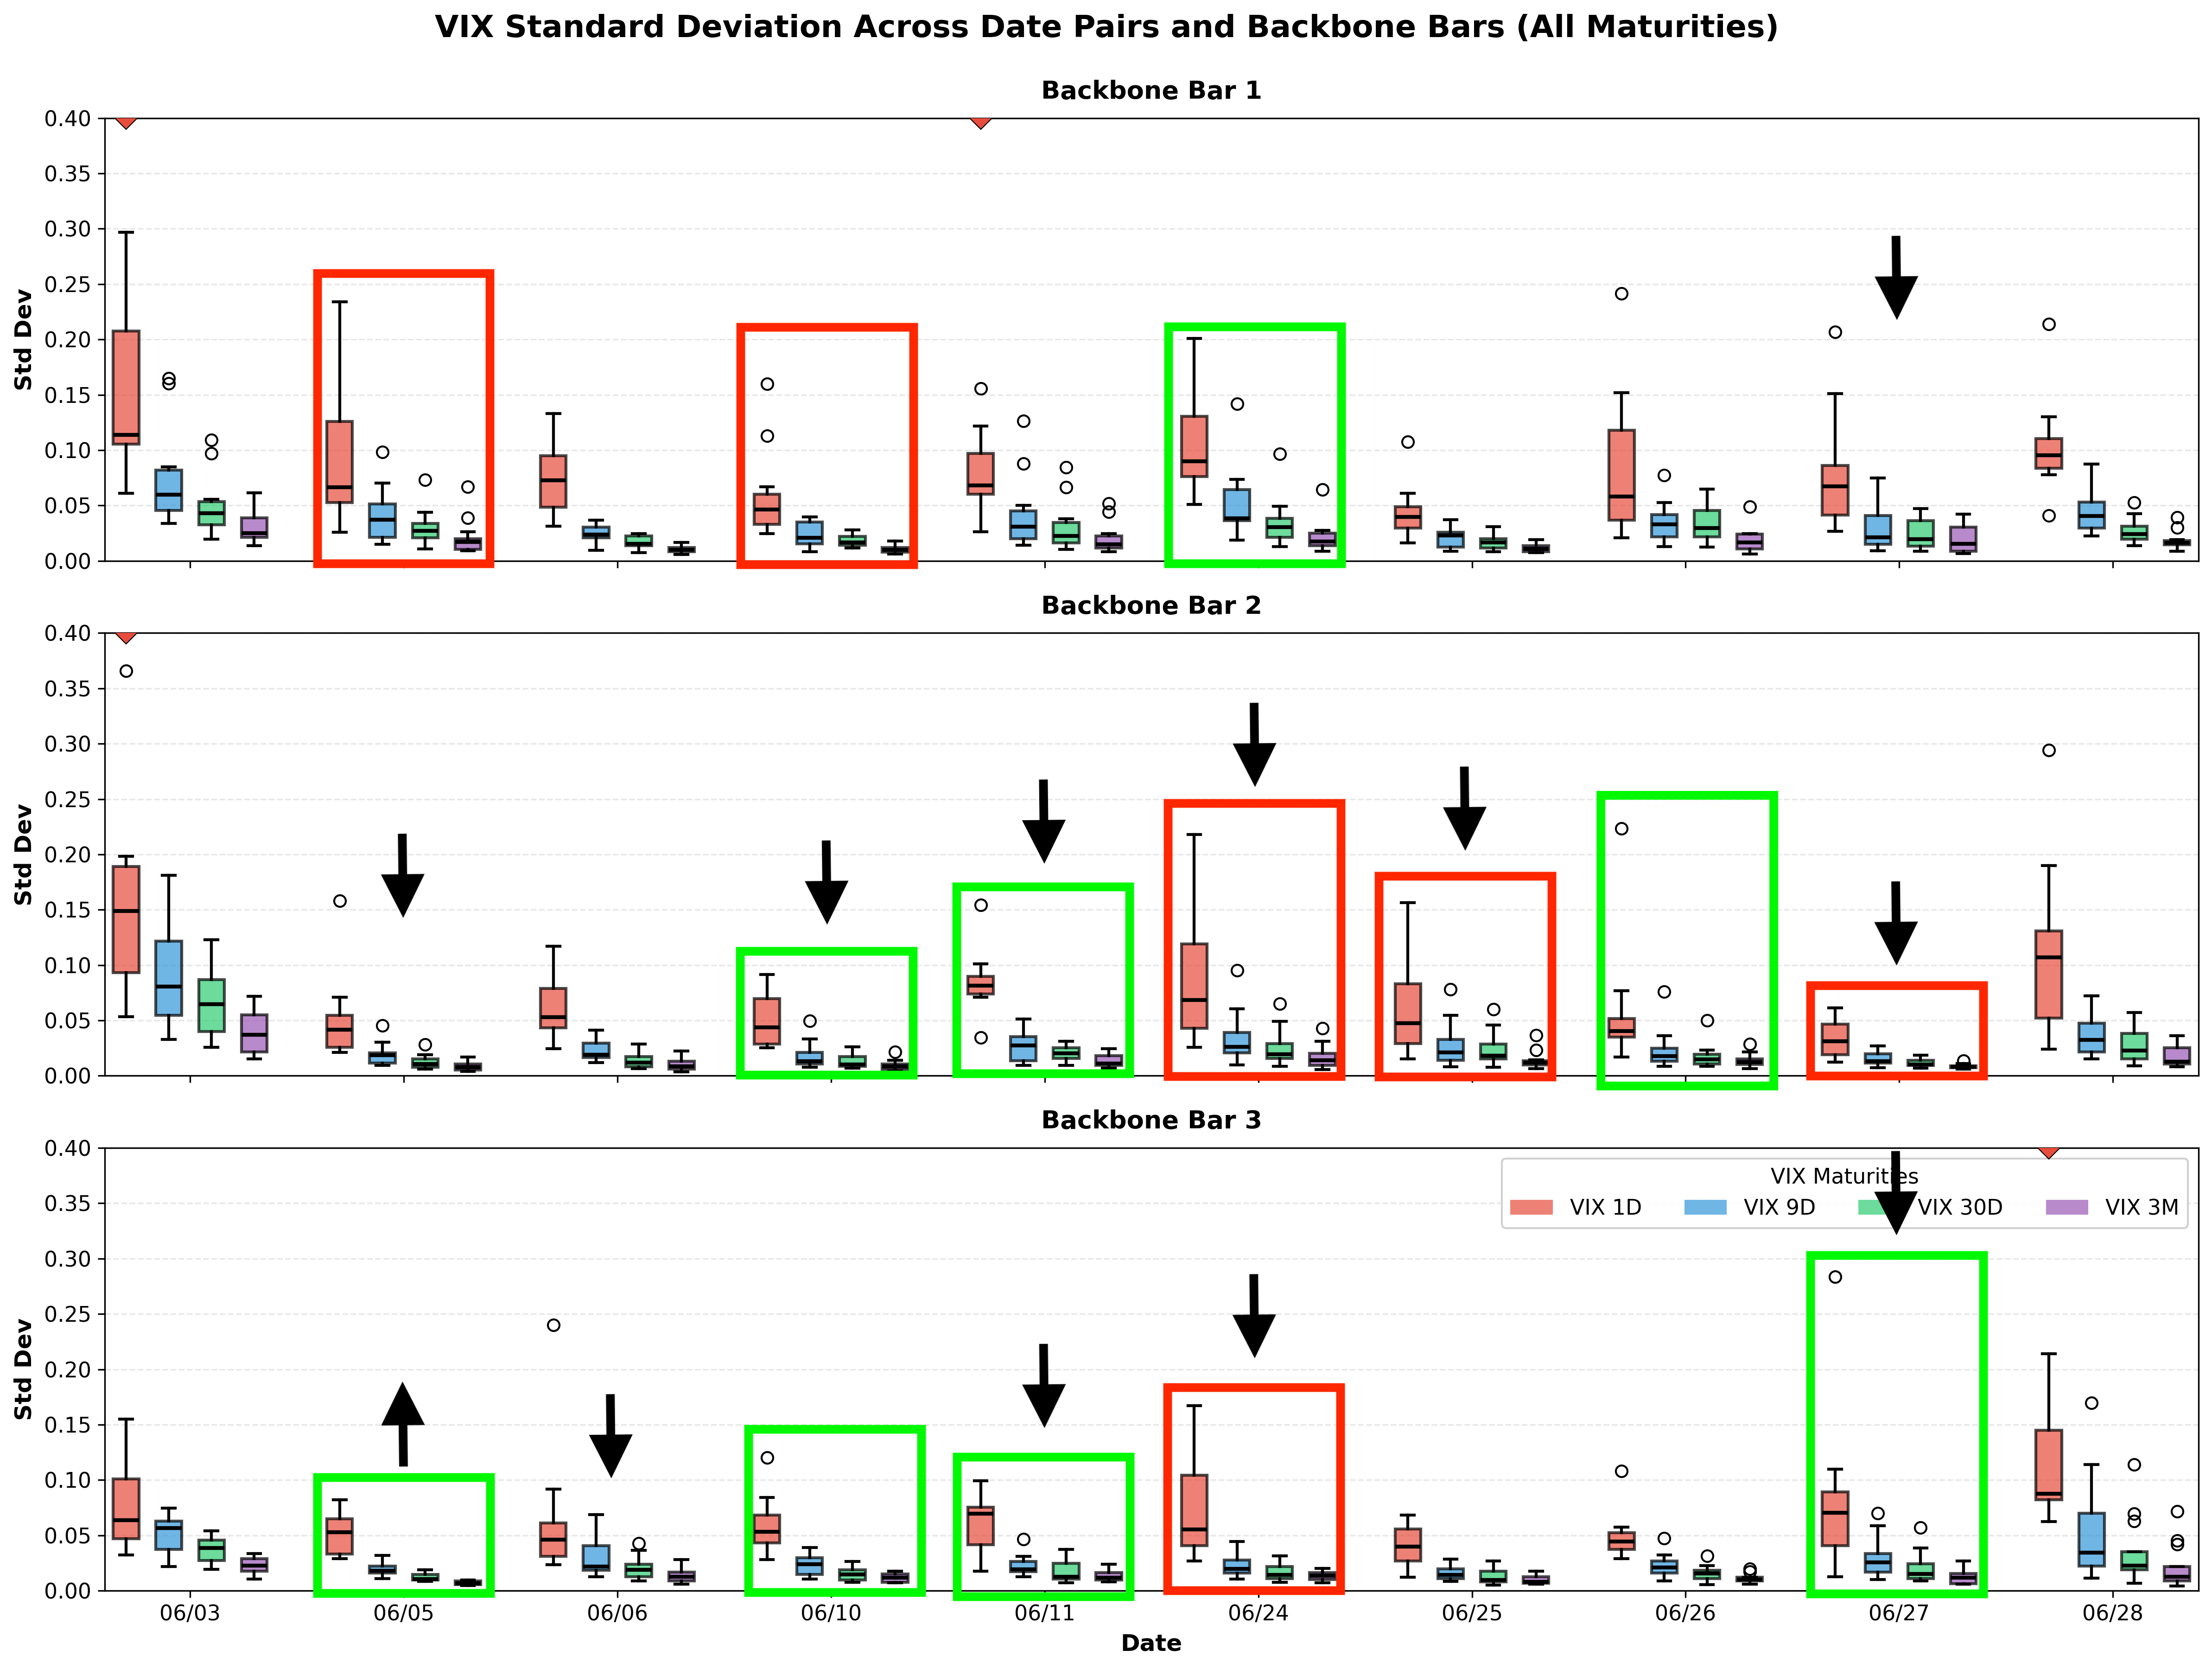
\includegraphics[width=0.9\linewidth]{vix_aggregate_std_boxplots_marked.png}
\caption{Distribution of the \textbf{standard deviation} of the VIX indices ($VIX_t^{(\tau)}$ for $\tau \in \{ \text{1d}, \text{9d}, \text{30d}, \text{3m} \}$) computed on each adapter bar and aggregated at the backbone bar level. See Figure~\ref{fig:sequential_boxplot_intc_data} for the interpretation of the markers.}
\label{fig:vix_aggregate_std}
\end{figure}

\begin{figure}[ht!]
\centering
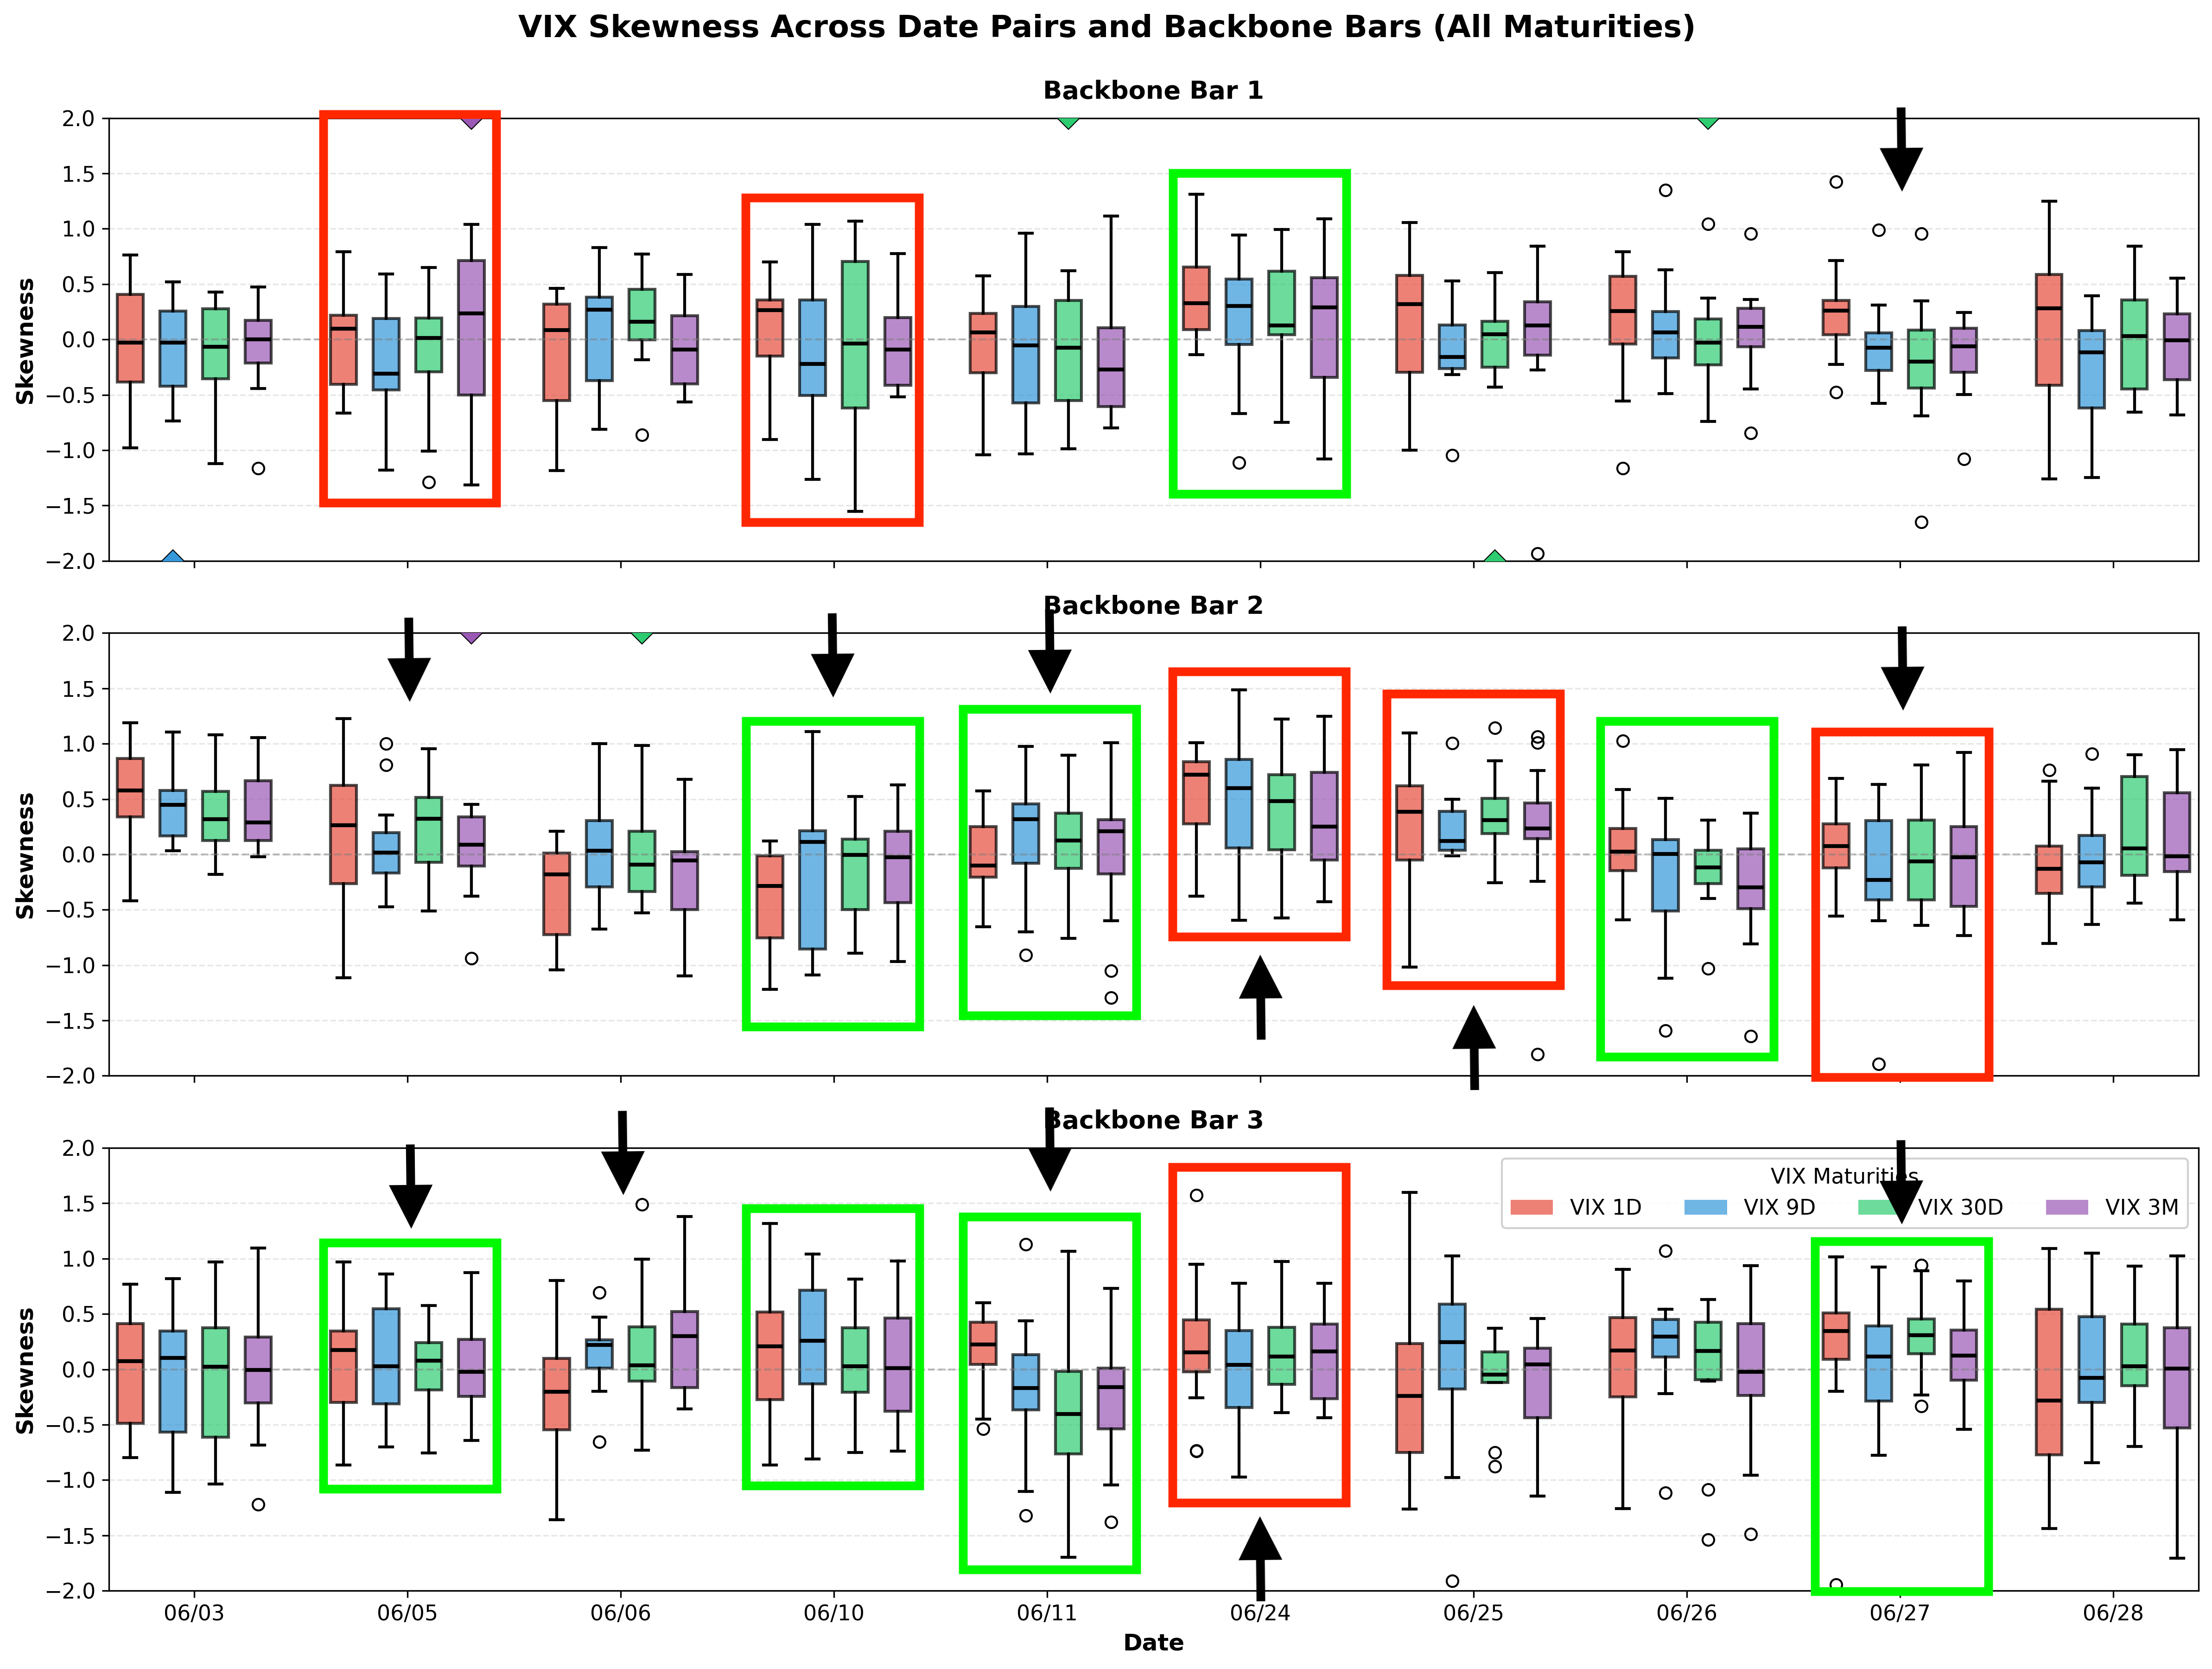
\includegraphics[width=0.9\linewidth]{vix_aggregate_skewness_boxplots_marked.png}
\caption{Distribution of the \textbf{skewness} of the VIX indices ($VIX_t^{(\tau)}$ for $\tau \in \{ \text{1d}, \text{9d}, \text{30d}, \text{3m} \}$) computed on each adapter bar and aggregated at the backbone bar level. See Figure~\ref{fig:sequential_boxplot_intc_data} for the interpretation of the markers.}
\label{fig:vix_aggregate_skewness}
\end{figure}

\begin{figure}[ht!]
\centering
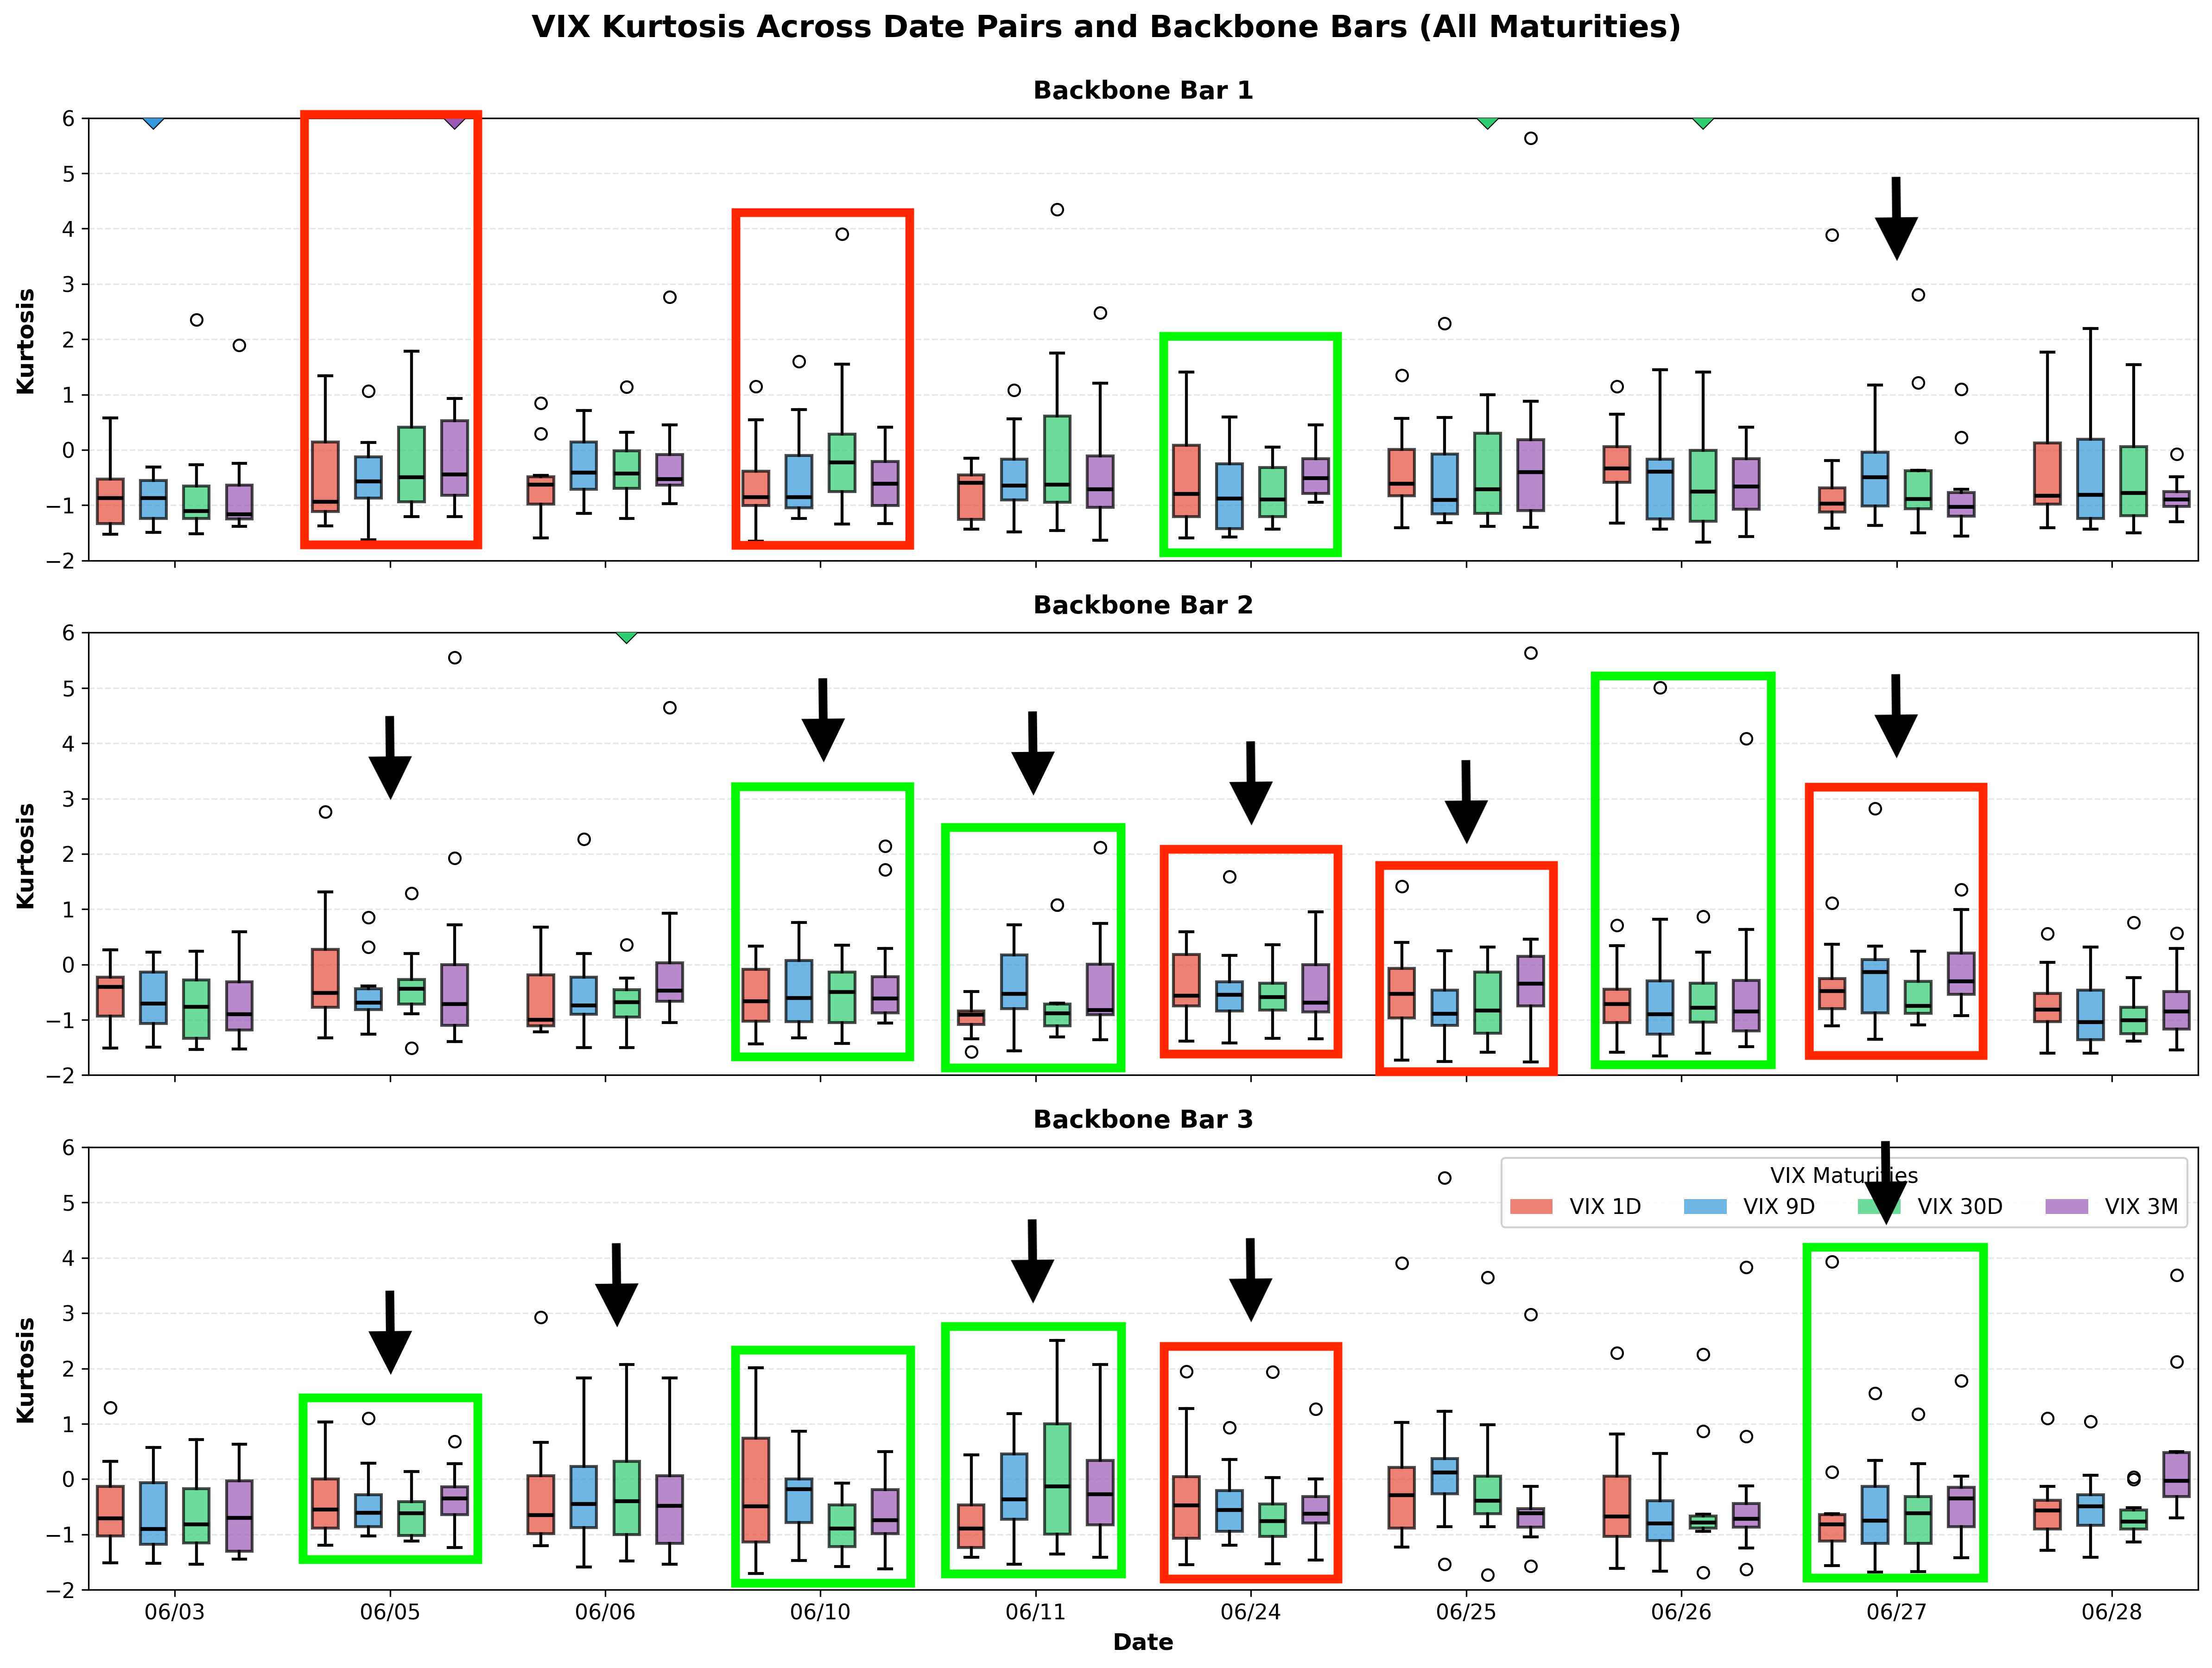
\includegraphics[width=0.9\linewidth]{vix_aggregate_kurtosis_boxplots_marked.png}
\caption{Distribution of the \textbf{kurtosis} of the VIX indices ($VIX_t^{(\tau)}$ for $\tau \in \{ \text{1d}, \text{9d}, \text{30d}, \text{3m} \}$) computed on each adapter bar and aggregated at the backbone bar level. See Figure~\ref{fig:sequential_boxplot_intc_data} for the interpretation of the markers.}
\label{fig:vix_aggregate_kurtosis}
\end{figure}

\begin{figure}[ht!]
\centering

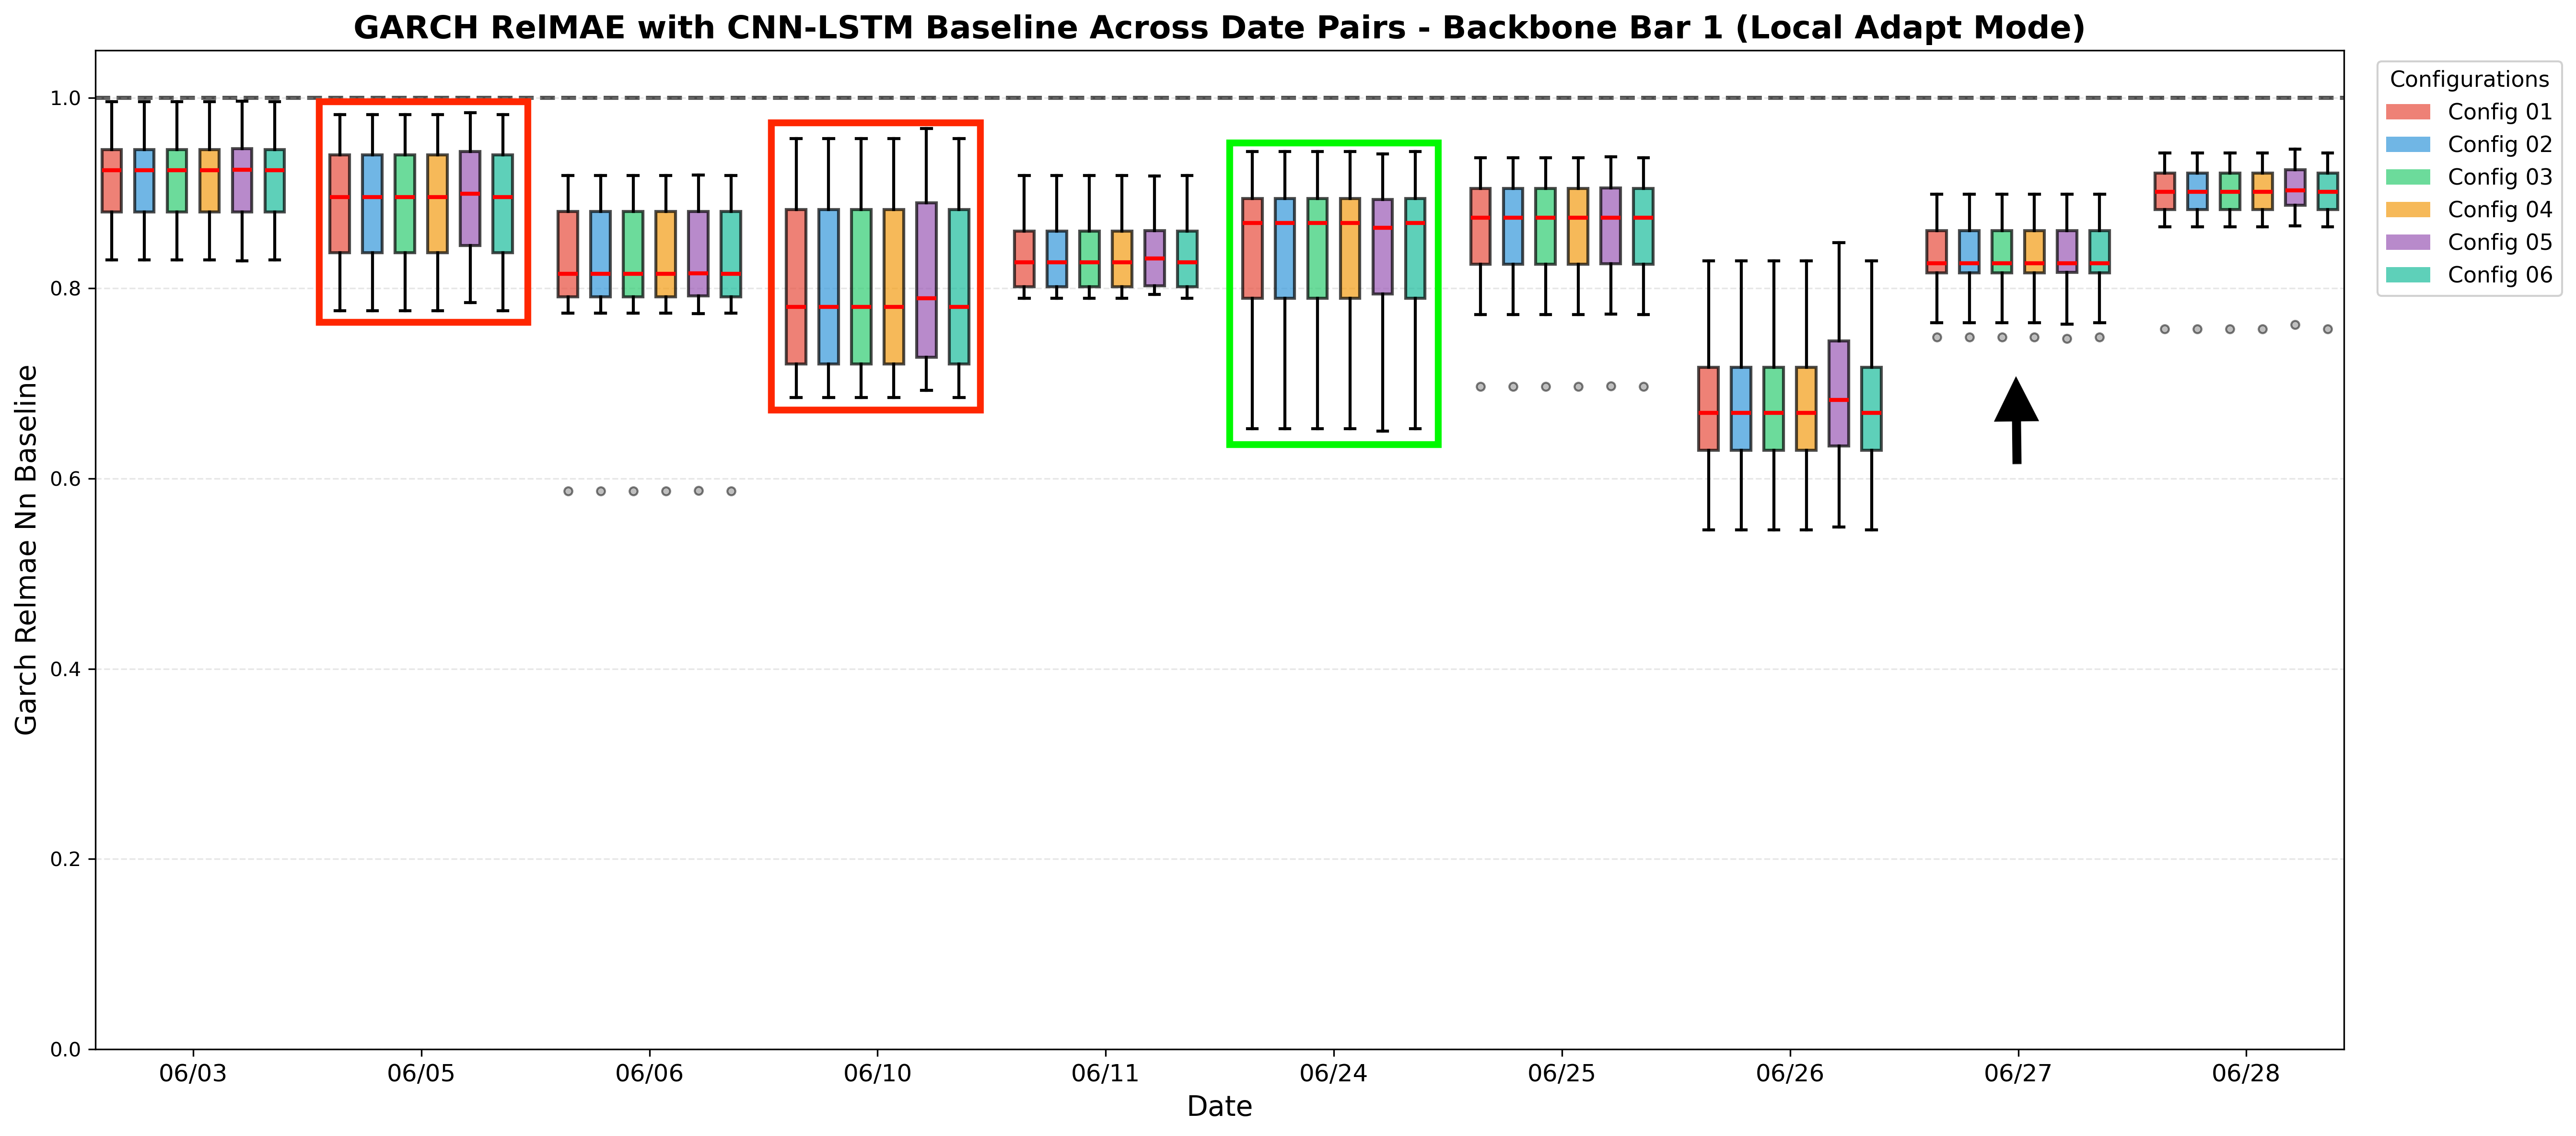
\includegraphics[width=0.9\linewidth]{sequential_boxplot_bb_000_nn_baseline_marked.png}
\vspace{0.5em}
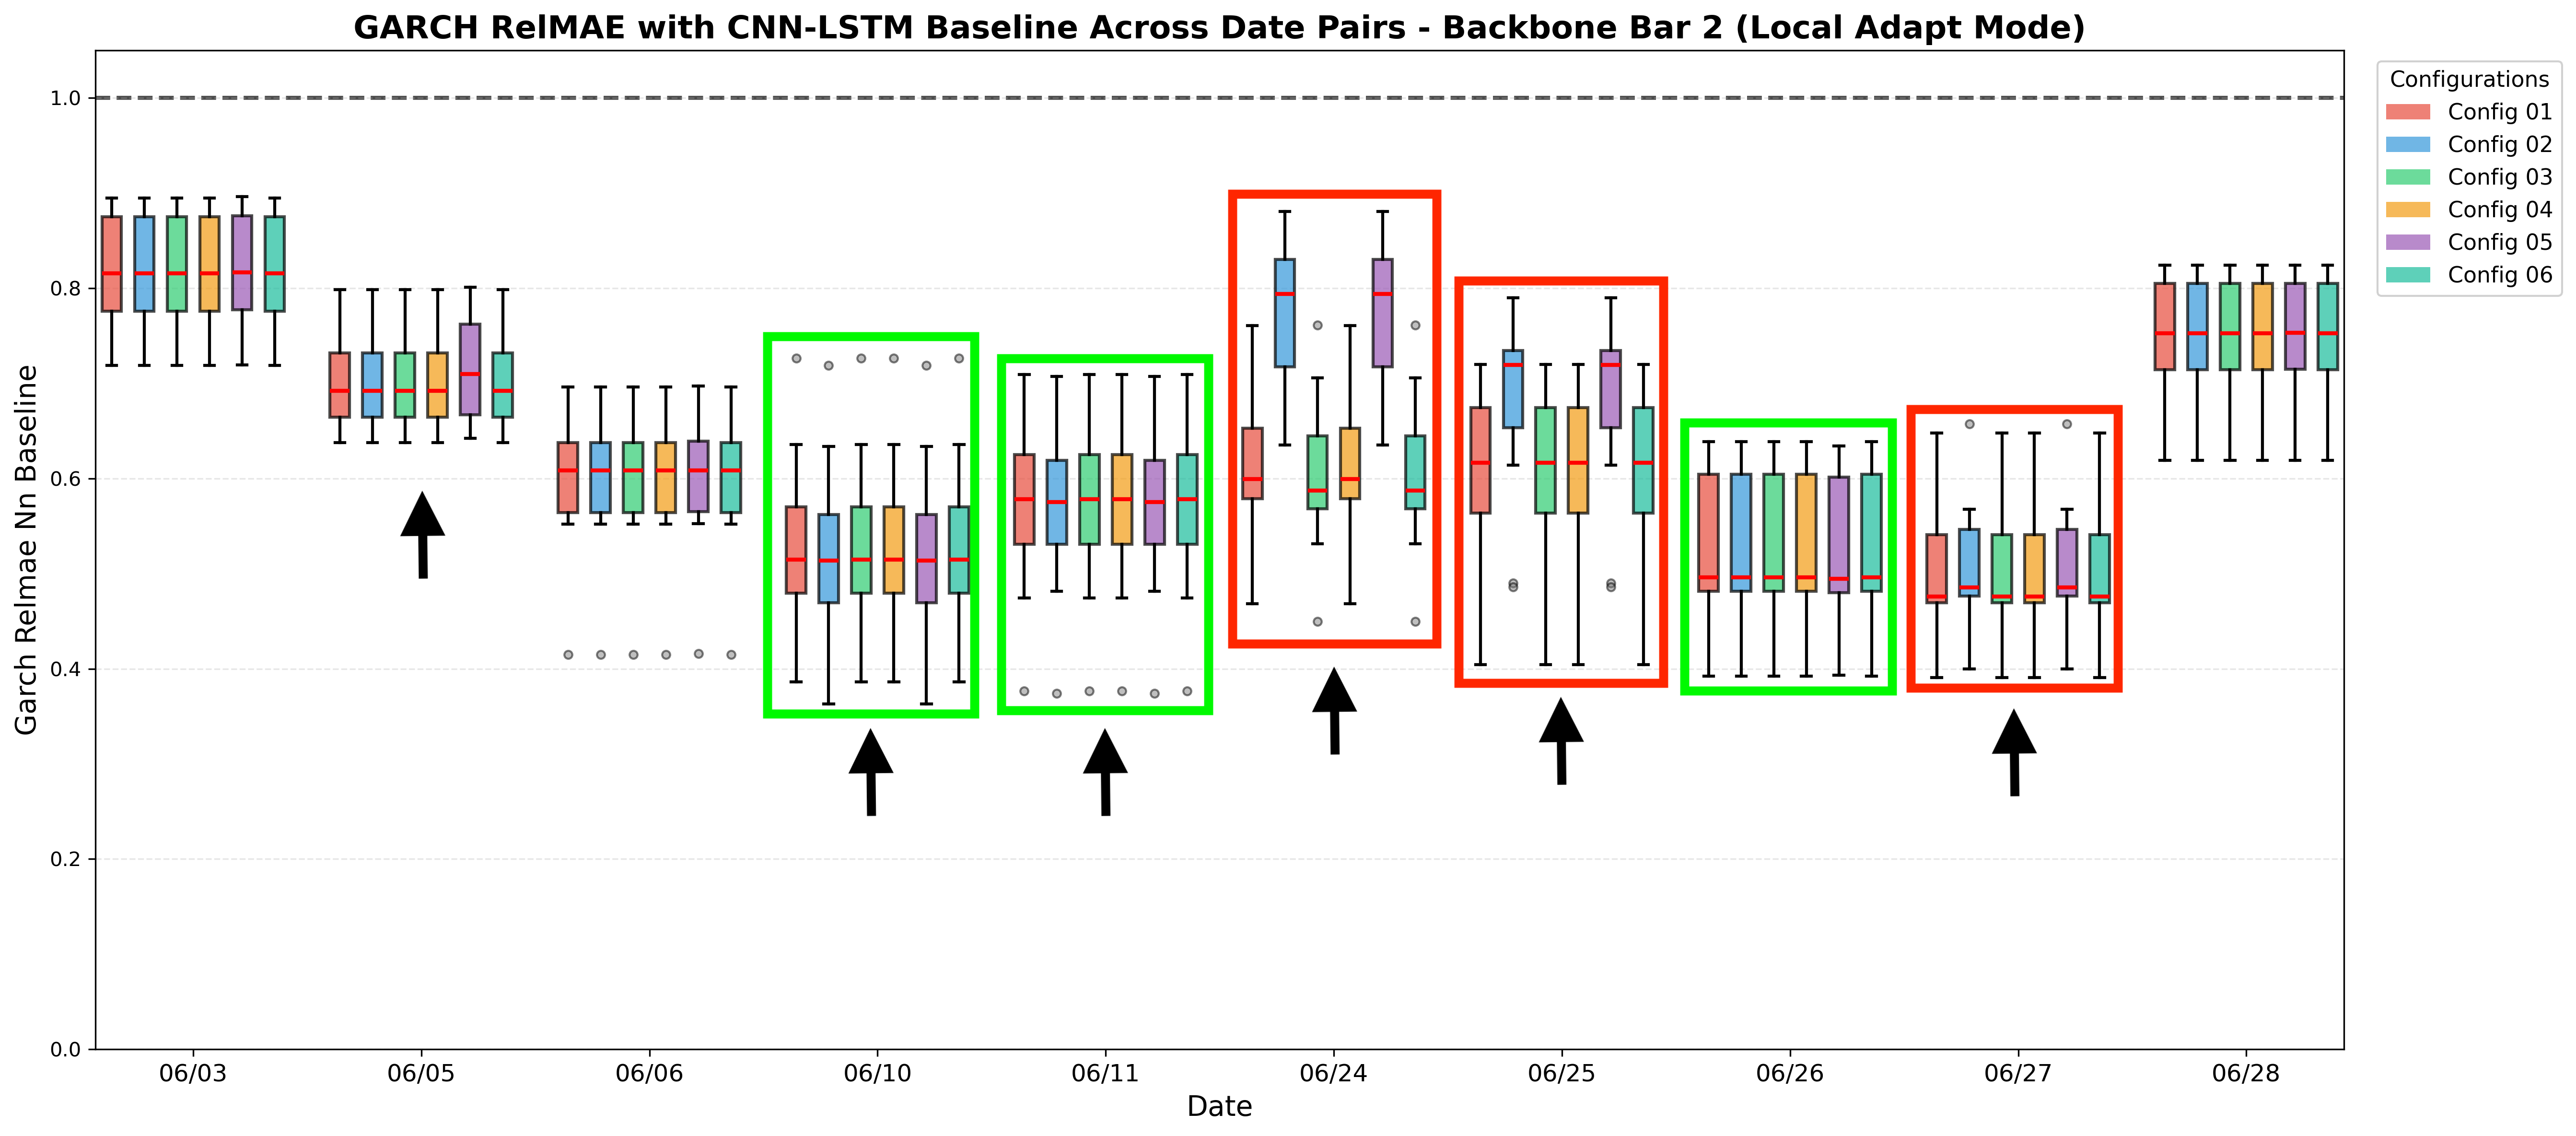
\includegraphics[width=0.9\linewidth]{sequential_boxplot_bb_001_nn_baseline_marked.png}
\vspace{0.5em}
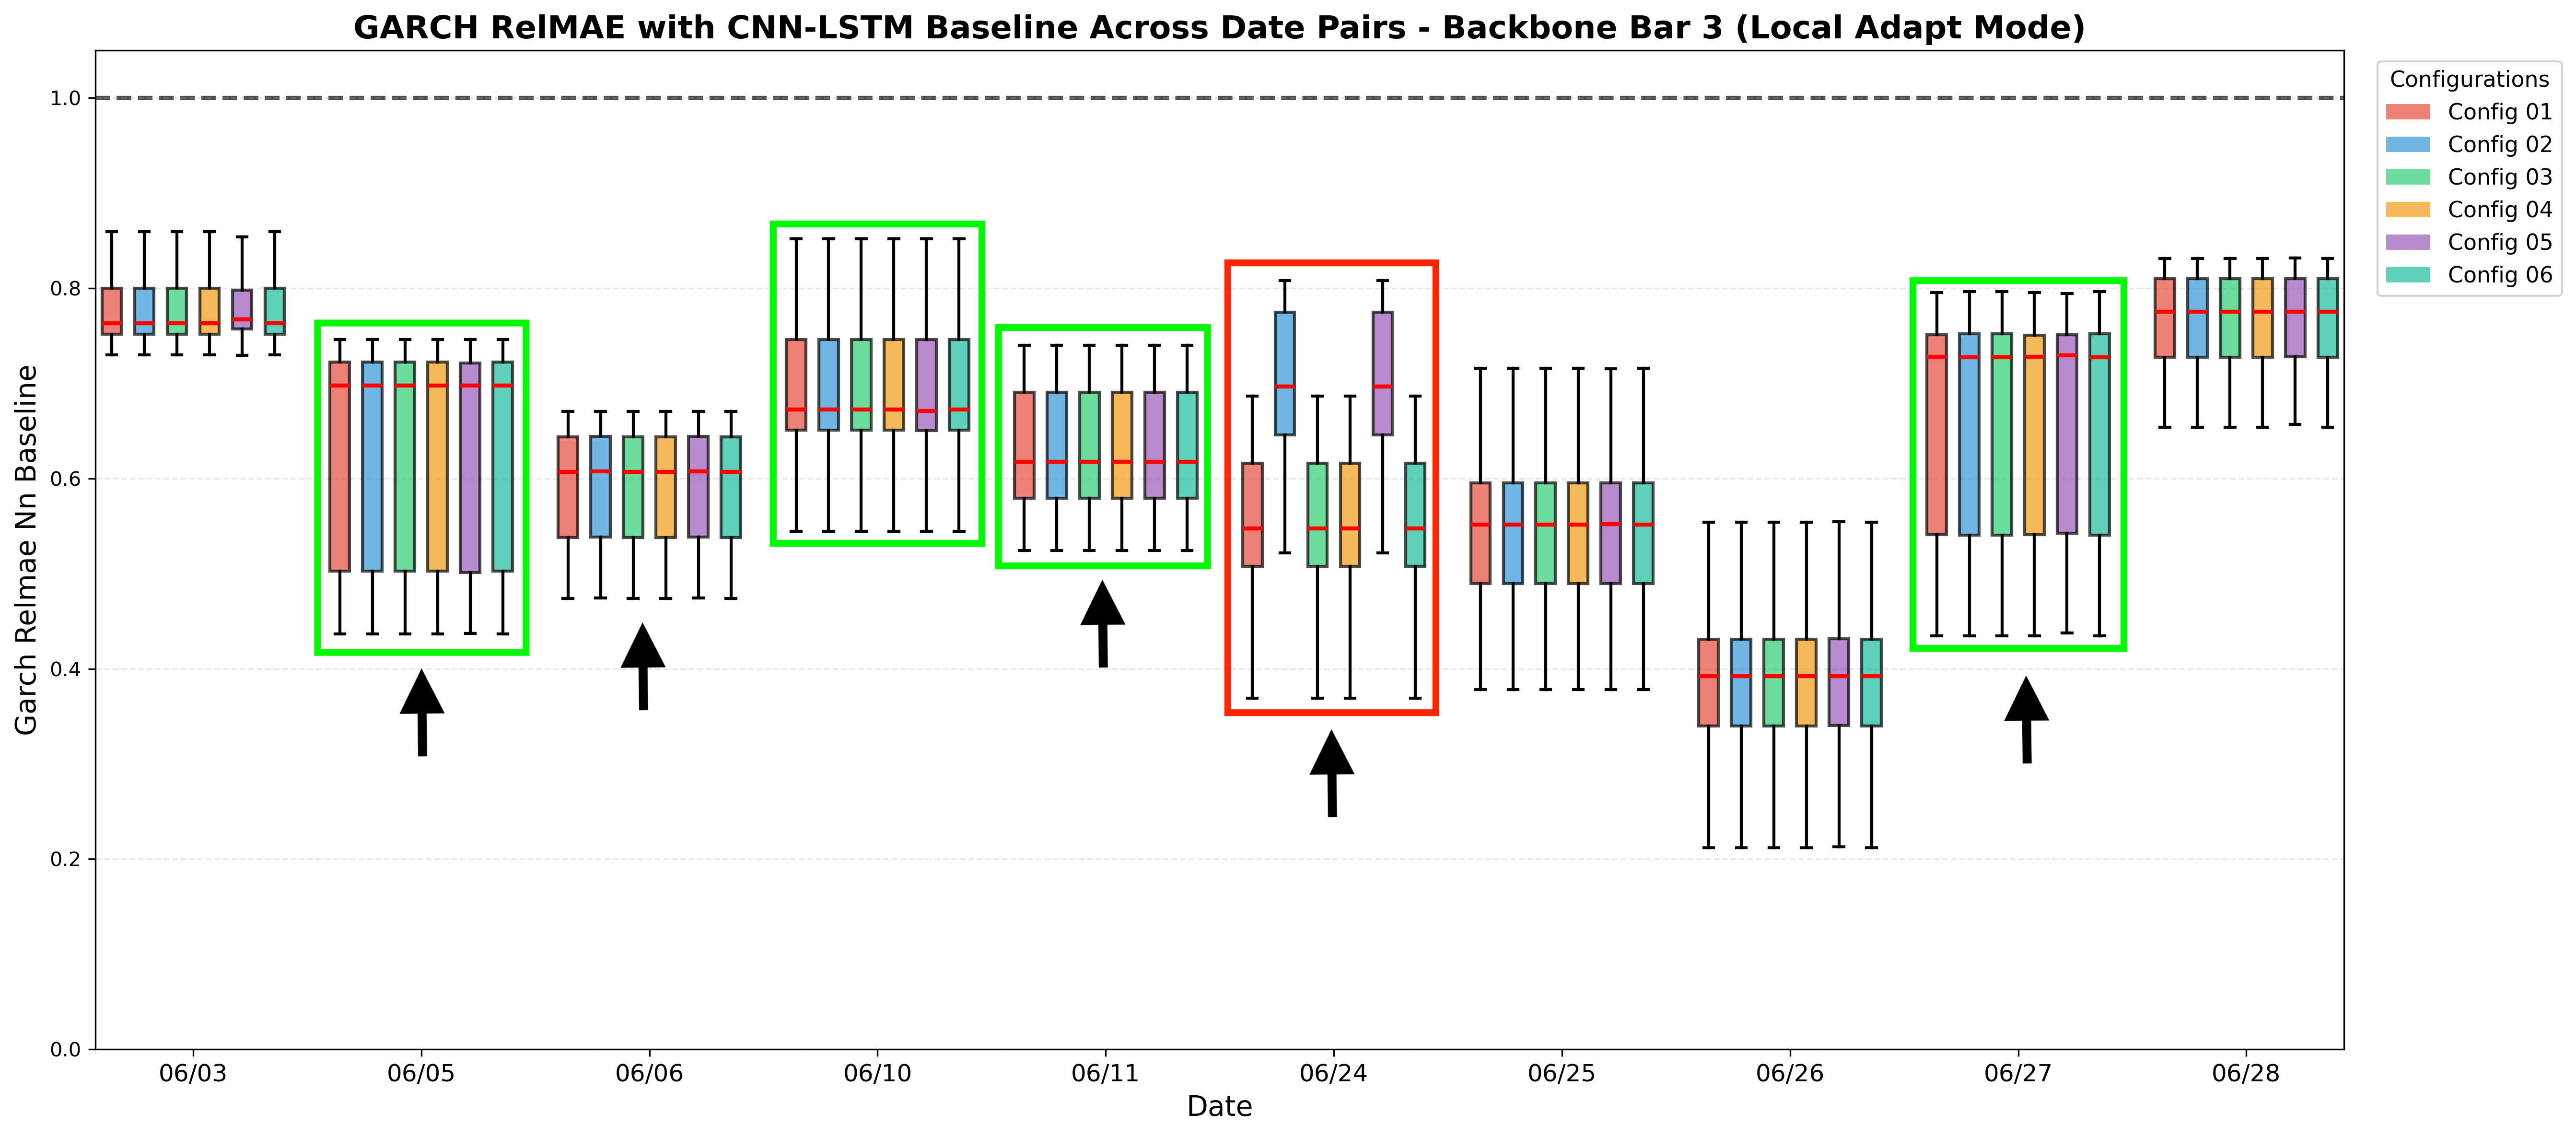
\includegraphics[width=0.9\linewidth]{sequential_boxplot_bb_002_nn_baseline_marked.png}

\caption{Sequential RelMAE boxplots for the INTC dataset across date pairs in Local Adapt mode using the raw CNN-LSTM imputation as the baseline (dashed line at 1.00). Top: Backbone Bar 1; Middle: Backbone Bar 2; Bottom: Backbone Bar 3. See Figure~\ref{fig:sequential_boxplot_intc_data} for the interpretation of the markers (arrows and rectangles).}
\label{fig:sequential_boxplot_intc_data_nn_baseline}
\end{figure}

% \begin{figure}[htb]
%   \centering
%   \includegraphics[width=4in]{param_series_PL3_04.png}
%   \caption{Evolution of parameter estimates for configuration \texttt{PL3\_04}. Blue lines denote combined estimates, while red dashed lines denote bar-specific estimates across adapter bars.}
%   \label{fig:param_series_pl3_04}
% \end{figure}

% \begin{figure}[htb]
%   \centering
%   \includegraphics[width=\linewidth]{armax_garch_corridor_M_03.png}
%   \caption{ARMAX–GARCH-DeepLOB corridor for model \texttt{SA\_04}. Cells show bar-specific coefficient magnitudes by adapter bar; asterisks mark statistical significance.}
%   \label{fig:armax_garch_corridor_M_03}
% \end{figure}


% \begin{figure}[htb]
%     \centering
%     \includegraphics[height=5in]{correlation_matrix_heatmap.png}  
%     \caption{Correlation matrix heatmap}
%     \label{fig:correlation_matrix}
% \end{figure}

% \begin{figure}[htb]
%     \centering
%     \includegraphics[height=4.5in]{arma_garch_coef_corridor.png}  
%     \caption{Corridor plot of purely endogenous ARMA(1, 1)-GARCH(1, 1) model. The numerical methods failed to converge on window 39.}
%     \label{fig:arma_garch_corridor}
% \end{figure}

% \begin{figure}[htb]
%     \centering
%     \includegraphics[height=4.5in]{reg_coef_corridor.png}  
%     \caption{Corridor plot of LASSO coefficients applied to the residuals of the purely endogenous model. Significant coefficients are indicated with $1$ in the corresponding tile.}
%     \label{fig:lasso_ols_corridor}
% \end{figure}

% \begin{figure}[htb]
%     \centering
%     \includegraphics[height=4in]{pos_neg_vs_sig_coefs.png} 
%     \caption{Count of windows where the coefficient is selected by the LASSO model (presence score) vs count of windows where the coefficient is statistically significant following the OLS regression.}
%     \label{fig:lasso_ols_scores}
% \end{figure}


% \begin{figure}[htb]
%     \centering
%     \includegraphics[height=4.5in]{armax_garch_coef_corridor.png} 
%     \caption{Corridor plot of the local coefficients of the Hybrid ARMAX(1, 1)-GARCH(1, 1) model. The optimization algorithms fail to converge on windows $3$ and $39$.}
%     \label{fig:armax_garch_corridor}
% \end{figure}


% \begin{figure}[htb]
%     \centering
%     \includegraphics[height=4in]{armax_garch_coef_evolution.png} 
%     \caption{Time series plot of the local ($\hat{\theta^{(i)}}$) and combined ($\hat{\theta^{(1 : i)}}$) parameter estimates.}
%     \label{fig:armax_garch_evolution}
% \end{figure}

% \begin{figure}[htb]
%     \centering
%     \includegraphics[height=5in]{gof_corridor.png} 
%     \caption{Goodness of fit tests corridor}
%     \label{fig:gof_corridor}
% \end{figure}

% \begin{figure}[htb]
%     \centering
%     \includegraphics[height=5in]{ccf_std_resid_ofi_itv.png} 
%     \caption{Cross correlation function of the Hybrid ARMAX-GARCH-DeepLOB model covariates.}
%     \label{fig:ccf_armax_garch}
% \end{figure}



% \begin{figure}[htb]
%     \centering
%     \includegraphics[height=4.5in]{armax_garch_coef_corridor_dl.png} 
%     \caption{Corridor plot of the local coefficients of the Hybrid ARMAX(1, 1)-GARCH(1, 1) model with distributed lags. The optimization algorithms fail to converge on windows $3$ and $39$.}
%     \label{fig:armax_garch_corridor_dl}
% \end{figure}


% \begin{figure}[htb]
%     \centering
%     \includegraphics[height=4in]{armax_garch_coef_evolution_dl.png} 
%     \caption{Time series plot of the local ($\hat{\theta^{(i)}}$) and combined ($\hat{\theta^{(1 : i)}}$) parameter estimates.}
%     \label{fig:armax_garch_evolution_dl}
% \end{figure}

% \begin{figure}[htb]
%     \centering
%     \includegraphics[height=5in]{gof_corridor_dl.png} 
%     \caption{Goodness of fit tests corridor}
%     \label{fig:gof_corridor_dl}
% \end{figure}

% \begin{figure}[htb]
%     \centering
%     \includegraphics[height=5in]{ccf_std_resid_ofi_itv_dl.png} 
%     \caption{Cross correlation function of the Hybrid ARMAX-GARCH-DeepLOB with distributed lags model covariates.}
%     \label{fig:ccf_armax_garch_dl}
% \end{figure}


\end{document}